\documentclass[twoside]{book}

% Packages required by doxygen
\usepackage{fixltx2e}
\usepackage{calc}
\usepackage{doxygen}
\usepackage[export]{adjustbox} % also loads graphicx
\usepackage{graphicx}
\usepackage[utf8]{inputenc}
\usepackage{makeidx}
\usepackage{multicol}
\usepackage{multirow}
\PassOptionsToPackage{warn}{textcomp}
\usepackage{textcomp}
\usepackage[nointegrals]{wasysym}
\usepackage[table]{xcolor}

% Font selection
\usepackage[T1]{fontenc}
\usepackage[scaled=.90]{helvet}
\usepackage{courier}
\usepackage{amssymb}
\usepackage{sectsty}
\renewcommand{\familydefault}{\sfdefault}
\allsectionsfont{%
  \fontseries{bc}\selectfont%
  \color{darkgray}%
}
\renewcommand{\DoxyLabelFont}{%
  \fontseries{bc}\selectfont%
  \color{darkgray}%
}
\newcommand{\+}{\discretionary{\mbox{\scriptsize$\hookleftarrow$}}{}{}}

% Page & text layout
\usepackage{geometry}
\geometry{%
  a4paper,%
  top=2.5cm,%
  bottom=2.5cm,%
  left=2.5cm,%
  right=2.5cm%
}
\tolerance=750
\hfuzz=15pt
\hbadness=750
\setlength{\emergencystretch}{15pt}
\setlength{\parindent}{0cm}
\setlength{\parskip}{3ex plus 2ex minus 2ex}
\makeatletter
\renewcommand{\paragraph}{%
  \@startsection{paragraph}{4}{0ex}{-1.0ex}{1.0ex}{%
    \normalfont\normalsize\bfseries\SS@parafont%
  }%
}
\renewcommand{\subparagraph}{%
  \@startsection{subparagraph}{5}{0ex}{-1.0ex}{1.0ex}{%
    \normalfont\normalsize\bfseries\SS@subparafont%
  }%
}
\makeatother

% Headers & footers
\usepackage{fancyhdr}
\pagestyle{fancyplain}
\fancyhead[LE]{\fancyplain{}{\bfseries\thepage}}
\fancyhead[CE]{\fancyplain{}{}}
\fancyhead[RE]{\fancyplain{}{\bfseries\leftmark}}
\fancyhead[LO]{\fancyplain{}{\bfseries\rightmark}}
\fancyhead[CO]{\fancyplain{}{}}
\fancyhead[RO]{\fancyplain{}{\bfseries\thepage}}
\fancyfoot[LE]{\fancyplain{}{}}
\fancyfoot[CE]{\fancyplain{}{}}
\fancyfoot[RE]{\fancyplain{}{\bfseries\scriptsize Generated by Doxygen }}
\fancyfoot[LO]{\fancyplain{}{\bfseries\scriptsize Generated by Doxygen }}
\fancyfoot[CO]{\fancyplain{}{}}
\fancyfoot[RO]{\fancyplain{}{}}
\renewcommand{\footrulewidth}{0.4pt}
\renewcommand{\chaptermark}[1]{%
  \markboth{#1}{}%
}
\renewcommand{\sectionmark}[1]{%
  \markright{\thesection\ #1}%
}

% Indices & bibliography
\usepackage{natbib}
\usepackage[titles]{tocloft}
\setcounter{tocdepth}{3}
\setcounter{secnumdepth}{5}
\makeindex

% Hyperlinks (required, but should be loaded last)
\usepackage{ifpdf}
\ifpdf
  \usepackage[pdftex,pagebackref=true]{hyperref}
\else
  \usepackage[ps2pdf,pagebackref=true]{hyperref}
\fi
\hypersetup{%
  colorlinks=true,%
  linkcolor=blue,%
  citecolor=blue,%
  unicode%
}

% Custom commands
\newcommand{\clearemptydoublepage}{%
  \newpage{\pagestyle{empty}\cleardoublepage}%
}

\usepackage{caption}
\captionsetup{labelsep=space,justification=centering,font={bf},singlelinecheck=off,skip=4pt,position=top}

%===== C O N T E N T S =====

\begin{document}

% Titlepage & ToC
\hypersetup{pageanchor=false,
             bookmarksnumbered=true,
             pdfencoding=unicode
            }
\pagenumbering{alph}
\begin{titlepage}
\vspace*{7cm}
\begin{center}%
{\Large Flow R\+OS \\[1ex]\large 0.\+1.\+0 }\\
\vspace*{1cm}
{\large Generated by Doxygen 1.8.13}\\
\end{center}
\end{titlepage}
\clearemptydoublepage
\pagenumbering{roman}
\tableofcontents
\clearemptydoublepage
\pagenumbering{arabic}
\hypersetup{pageanchor=true}

%--- Begin generated contents ---
\chapter{Flow-\/\+R\+OS}
\label{index}\hypertarget{index}{}This library is meant for synchronizing multiple series of R\+OS messages, collected by {\ttfamily ros\+::\+Subscriber} objects. This is typically desirable in R\+OS nodes where multiple inputs are required to compute something, and the computed result is accurate only if the inputs have consistent relative sequencing. This library uses \href{https://github.com/fetchrobotics/flow}{\tt Flow} to fulfill these requirements in a customizable way.

Secondarily, this library provides in-\/process subscriber/publisher mechanisms which do not require a running R\+OS core and are swappable with their R\+O\+S-\/enabled counterparts. These are especially useful for testing message passing subsystems. 
\chapter{Namespace Index}
\section{Namespace List}
Here is a list of all documented namespaces with brief descriptions\+:\begin{DoxyCompactList}
\item\contentsline{section}{\hyperlink{namespaceflow__ros}{flow\+\_\+ros} }{\pageref{namespaceflow__ros}}{}
\end{DoxyCompactList}

\chapter{Hierarchical Index}
\section{Class Hierarchy}
This inheritance list is sorted roughly, but not completely, alphabetically\+:\begin{DoxyCompactList}
\item \contentsline{section}{Callback\+Object}{\pageref{struct_callback_object}}{}
\item \contentsline{section}{flow\+\_\+ros\+:\+:Event\+Handler$<$ Publisher\+Tuple, Subscriber\+Tuple, Output\+Container\+Type\+Info\+Tmpl $>$\+:\+:Callbacks}{\pageref{structflow__ros_1_1_event_handler_1_1_callbacks}}{}
\item Captor\+Traits\begin{DoxyCompactList}
\item \contentsline{section}{flow\+:\+:Captor\+Traits$<$\+:\+:flow\+\_\+ros\+:\+:Subscriber$<$ MsgT, Policy\+Tmpl, Lock\+PolicyT $>$ $>$}{\pageref{structflow_1_1_captor_traits_3_1_1flow__ros_1_1_subscriber_3_01_msg_t_00_01_policy_tmpl_00_01_lock_policy_t_01_4_01_4}}{}
\item \contentsline{section}{flow\+:\+:Captor\+Traits$<$\+:\+:flow\+\_\+ros\+:\+:Subscriber\+Policy\+Base$<$ PolicyT $>$ $>$}{\pageref{structflow_1_1_captor_traits_3_1_1flow__ros_1_1_subscriber_policy_base_3_01_policy_t_01_4_01_4}}{}
\end{DoxyCompactList}
\item \contentsline{section}{flow\+\_\+ros\+:\+:detail\+:\+:Collect\+From\+Tuple$<$ Output\+IteratorT $>$}{\pageref{classflow__ros_1_1detail_1_1_collect_from_tuple}}{}
\item \contentsline{section}{flow\+\_\+ros\+:\+:Default\+Message\+Seq\+Dispatch\+Access}{\pageref{structflow__ros_1_1_default_message_seq_dispatch_access}}{}
\begin{DoxyCompactList}
\item \contentsline{section}{flow\+:\+:Dispatch\+Access$<$ MsgT $>$}{\pageref{structflow_1_1_dispatch_access}}{}
\end{DoxyCompactList}
\item \contentsline{section}{flow\+\_\+ros\+:\+:Default\+Message\+Stamp\+Dispatch\+Access}{\pageref{structflow__ros_1_1_default_message_stamp_dispatch_access}}{}
\begin{DoxyCompactList}
\item \contentsline{section}{flow\+:\+:Dispatch\+Access$<$ MsgT $>$}{\pageref{structflow_1_1_dispatch_access}}{}
\end{DoxyCompactList}
\item \contentsline{section}{flow\+\_\+ros\+:\+:Default\+Output\+Container\+Type\+Info$<$ DispatchT $>$}{\pageref{structflow__ros_1_1_default_output_container_type_info}}{}
\item \contentsline{section}{flow\+:\+:Dispatch\+Traits$<$ boost\+:\+:shared\+\_\+ptr$<$ const MsgT $>$ $>$}{\pageref{structflow_1_1_dispatch_traits_3_01boost_1_1shared__ptr_3_01const_01_msg_t_01_4_01_4}}{}
\item \contentsline{section}{flow\+:\+:Dispatch\+Traits$<$ std\+:\+:shared\+\_\+ptr$<$ const MsgT $>$ $>$}{\pageref{structflow_1_1_dispatch_traits_3_01std_1_1shared__ptr_3_01const_01_msg_t_01_4_01_4}}{}
\item \contentsline{section}{flow\+\_\+ros\+:\+:Event\+Handler\+Base}{\pageref{classflow__ros_1_1_event_handler_base}}{}
\begin{DoxyCompactList}
\item \contentsline{section}{flow\+\_\+ros\+:\+:Event\+Handler$<$ Publisher\+Tuple, Subscriber\+Tuple, Output\+Container\+Type\+Info\+Tmpl $>$}{\pageref{classflow__ros_1_1_event_handler}}{}
\end{DoxyCompactList}
\item \contentsline{section}{flow\+\_\+ros\+:\+:detail\+:\+:Event\+Handler\+Input\+Type$<$ Output\+Container\+Type\+Info\+Tmpl, Subscriber\+Tuple\+Type $>$}{\pageref{structflow__ros_1_1detail_1_1_event_handler_input_type}}{}
\item \contentsline{section}{flow\+\_\+ros\+:\+:detail\+:\+:Event\+Handler\+Input\+Type$<$ Output\+Container\+Type\+Info\+Tmpl, std\+:\+:tuple$<$ Subscriber\+Ts... $>$ $>$}{\pageref{structflow__ros_1_1detail_1_1_event_handler_input_type_3_01_output_container_type_info_tmpl_00_0ffddcead573ab44a62afad7bf9d6e18f}}{}
\item \contentsline{section}{flow\+\_\+ros\+:\+:detail\+:\+:Event\+Handler\+Output\+Type$<$ Publisher\+TupleT $>$}{\pageref{structflow__ros_1_1detail_1_1_event_handler_output_type}}{}
\item \contentsline{section}{flow\+\_\+ros\+:\+:detail\+:\+:Event\+Handler\+Output\+Type$<$ std\+:\+:tuple$<$ Publisher\+Ts... $>$ $>$}{\pageref{structflow__ros_1_1detail_1_1_event_handler_output_type_3_01std_1_1tuple_3_01_publisher_ts_8_8_8_01_4_01_4}}{}
\item \contentsline{section}{flow\+\_\+ros\+:\+:detail\+:\+:Event\+Handler\+Output\+Type$<$ std\+:\+:tuple$<$$>$ $>$}{\pageref{structflow__ros_1_1detail_1_1_event_handler_output_type_3_01std_1_1tuple_3_4_01_4}}{}
\item \contentsline{section}{flow\+\_\+ros\+:\+:detail\+:\+:Event\+Handler\+Publish\+Helper}{\pageref{classflow__ros_1_1detail_1_1_event_handler_publish_helper}}{}
\item \contentsline{section}{flow\+\_\+ros\+:\+:Event\+Summary}{\pageref{structflow__ros_1_1_event_summary}}{}
\item exception\begin{DoxyCompactList}
\item \contentsline{section}{flow\+\_\+ros\+:\+:routing\+:\+:Message\+Instance\+Error}{\pageref{classflow__ros_1_1routing_1_1_message_instance_error}}{}
\item \contentsline{section}{flow\+\_\+ros\+:\+:routing\+:\+:Message\+Type\+Error}{\pageref{classflow__ros_1_1routing_1_1_message_type_error}}{}
\item \contentsline{section}{flow\+\_\+ros\+:\+:Unknown\+Subscription\+Error}{\pageref{classflow__ros_1_1_unknown_subscription_error}}{}
\end{DoxyCompactList}
\item is\+\_\+driver\begin{DoxyCompactList}
\item \contentsline{section}{flow\+:\+:is\+\_\+driver$<$\+:\+:flow\+\_\+ros\+:\+:Subscriber$<$ MsgT, Policy\+Tmpl, Lock\+PolicyT $>$ $>$}{\pageref{structflow_1_1is__driver_3_1_1flow__ros_1_1_subscriber_3_01_msg_t_00_01_policy_tmpl_00_01_lock_policy_t_01_4_01_4}}{}
\end{DoxyCompactList}
\item is\+\_\+follower\begin{DoxyCompactList}
\item \contentsline{section}{flow\+:\+:is\+\_\+follower$<$\+:\+:flow\+\_\+ros\+:\+:Subscriber$<$ MsgT, Policy\+Tmpl, Lock\+PolicyT $>$ $>$}{\pageref{structflow_1_1is__follower_3_1_1flow__ros_1_1_subscriber_3_01_msg_t_00_01_policy_tmpl_00_01_lock_policy_t_01_4_01_4}}{}
\end{DoxyCompactList}
\item \contentsline{section}{flow\+\_\+ros\+:\+:routing\+:\+:Local\+Publication\+Base}{\pageref{classflow__ros_1_1routing_1_1_local_publication_base}}{}
\begin{DoxyCompactList}
\item \contentsline{section}{flow\+\_\+ros\+:\+:routing\+:\+:Local\+Publication$<$ MsgT $>$}{\pageref{classflow__ros_1_1routing_1_1_local_publication}}{}
\end{DoxyCompactList}
\item \contentsline{section}{flow\+\_\+ros\+:\+:routing\+:\+:Local\+Subscription\+Base}{\pageref{classflow__ros_1_1routing_1_1_local_subscription_base}}{}
\begin{DoxyCompactList}
\item \contentsline{section}{flow\+\_\+ros\+:\+:routing\+:\+:Local\+Subscription$<$ MsgT $>$}{\pageref{classflow__ros_1_1routing_1_1_local_subscription}}{}
\end{DoxyCompactList}
\item \contentsline{section}{flow\+\_\+ros\+:\+:routing\+:\+:Local\+Subscription\+Group}{\pageref{classflow__ros_1_1routing_1_1_local_subscription_group}}{}
\item \contentsline{section}{flow\+\_\+ros\+:\+:Message\+Shared\+Const\+Ptr\+Type$<$ MsgT, I\+S\+\_\+\+R\+O\+S\+\_\+\+M\+E\+S\+S\+A\+GE $>$}{\pageref{structflow__ros_1_1_message_shared_const_ptr_type}}{}
\item \contentsline{section}{flow\+\_\+ros\+:\+:Message\+Shared\+Const\+Ptr\+Type$<$ MsgT, true $>$}{\pageref{structflow__ros_1_1_message_shared_const_ptr_type_3_01_msg_t_00_01true_01_4}}{}
\item \contentsline{section}{flow\+\_\+ros\+:\+:Message\+Shared\+Ptr\+Type$<$ MsgT, I\+S\+\_\+\+R\+O\+S\+\_\+\+M\+E\+S\+S\+A\+GE $>$}{\pageref{structflow__ros_1_1_message_shared_ptr_type}}{}
\item \contentsline{section}{flow\+\_\+ros\+:\+:Message\+Shared\+Ptr\+Type$<$ MsgT, true $>$}{\pageref{structflow__ros_1_1_message_shared_ptr_type_3_01_msg_t_00_01true_01_4}}{}
\item Policy\+Tmpl\begin{DoxyCompactList}
\item \contentsline{section}{flow\+\_\+ros\+:\+:Subscriber\+Policy\+Base$<$ Policy\+Tmpl$<$ message\+\_\+shared\+\_\+const\+\_\+ptr\+\_\+t$<$ const MsgT $>$, Lock\+PolicyT, Msg\+Const\+Ptr\+ContainerT $>$ $>$}{\pageref{classflow__ros_1_1_subscriber_policy_base}}{}
\begin{DoxyCompactList}
\item \contentsline{section}{flow\+\_\+ros\+:\+:Subscriber$<$ MsgT, Policy\+Tmpl, Lock\+PolicyT, Msg\+Const\+Ptr\+ContainerT $>$}{\pageref{classflow__ros_1_1_subscriber}}{}
\end{DoxyCompactList}
\end{DoxyCompactList}
\item \contentsline{section}{flow\+\_\+ros\+:\+:routing\+:\+:Publication\+Wrapper$<$ MsgT $>$}{\pageref{classflow__ros_1_1routing_1_1_publication_wrapper}}{}
\begin{DoxyCompactList}
\item \contentsline{section}{flow\+\_\+ros\+:\+:routing\+:\+:Local\+Publication$<$ MsgT $>$}{\pageref{classflow__ros_1_1routing_1_1_local_publication}}{}
\item \contentsline{section}{flow\+\_\+ros\+:\+:routing\+:\+:R\+O\+S\+Publication$<$ MsgT $>$}{\pageref{classflow__ros_1_1routing_1_1_r_o_s_publication}}{}
\end{DoxyCompactList}
\item \contentsline{section}{flow\+\_\+ros\+:\+:Publisher\+Base}{\pageref{classflow__ros_1_1_publisher_base}}{}
\begin{DoxyCompactList}
\item \contentsline{section}{flow\+\_\+ros\+:\+:Publisher\+Output\+Base$<$ MsgT $>$}{\pageref{classflow__ros_1_1_publisher_output_base}}{}
\begin{DoxyCompactList}
\item \contentsline{section}{flow\+\_\+ros\+:\+:Multi\+Publisher$<$ MsgT, Output\+ContainerT $>$}{\pageref{classflow__ros_1_1_multi_publisher}}{}
\item \contentsline{section}{flow\+\_\+ros\+:\+:Publisher$<$ MsgT $>$}{\pageref{classflow__ros_1_1_publisher}}{}
\end{DoxyCompactList}
\end{DoxyCompactList}
\item \contentsline{section}{flow\+\_\+ros\+:\+:Publisher\+Traits$<$ MsgT $>$}{\pageref{structflow__ros_1_1_publisher_traits}}{}
\item \contentsline{section}{flow\+\_\+ros\+:\+:Publisher\+Traits$<$ Multi\+Publisher$<$ MsgT, Output\+ContainerT $>$ $>$}{\pageref{structflow__ros_1_1_publisher_traits_3_01_multi_publisher_3_01_msg_t_00_01_output_container_t_01_4_01_4}}{}
\item \contentsline{section}{flow\+\_\+ros\+:\+:Publisher\+Traits$<$ Publisher$<$ MsgT $>$ $>$}{\pageref{structflow__ros_1_1_publisher_traits_3_01_publisher_3_01_msg_t_01_4_01_4}}{}
\item \contentsline{section}{flow\+\_\+ros\+:\+:detail\+:\+:Retry\+Reinject\+Helper}{\pageref{structflow__ros_1_1detail_1_1_retry_reinject_helper}}{}
\item \contentsline{section}{flow\+\_\+ros\+:\+:Router}{\pageref{classflow__ros_1_1_router}}{}
\item \contentsline{section}{flow\+\_\+ros\+:\+:Stamp\+Setter$<$ MsgT $>$}{\pageref{structflow__ros_1_1_stamp_setter}}{}
\item \contentsline{section}{flow\+:\+:Stamp\+Traits$<$ ros\+:\+:Time $>$}{\pageref{structflow_1_1_stamp_traits_3_01ros_1_1_time_01_4}}{}
\item \contentsline{section}{flow\+\_\+ros\+:\+:Subscriber\+Base}{\pageref{classflow__ros_1_1_subscriber_base}}{}
\begin{DoxyCompactList}
\item \contentsline{section}{flow\+\_\+ros\+:\+:Subscriber\+Policy\+Base$<$ PolicyT $>$}{\pageref{classflow__ros_1_1_subscriber_policy_base}}{}
\item \contentsline{section}{flow\+\_\+ros\+:\+:Subscriber\+Policy\+Base$<$ Policy\+Tmpl$<$ message\+\_\+shared\+\_\+const\+\_\+ptr\+\_\+t$<$ const MsgT $>$, Lock\+PolicyT, Msg\+Const\+Ptr\+ContainerT $>$ $>$}{\pageref{classflow__ros_1_1_subscriber_policy_base}}{}
\end{DoxyCompactList}
\item \contentsline{section}{flow\+\_\+ros\+:\+:Subscriber\+Traits$<$ MsgT $>$}{\pageref{structflow__ros_1_1_subscriber_traits}}{}
\item \contentsline{section}{flow\+\_\+ros\+:\+:Subscriber\+Traits$<$ Subscriber$<$ MsgT, Policy\+Tmpl, Lock\+PolicyT $>$ $>$}{\pageref{structflow__ros_1_1_subscriber_traits_3_01_subscriber_3_01_msg_t_00_01_policy_tmpl_00_01_lock_policy_t_01_4_01_4}}{}
\item \contentsline{section}{flow\+\_\+ros\+:\+:routing\+:\+:Subscription\+Wrapper}{\pageref{classflow__ros_1_1routing_1_1_subscription_wrapper}}{}
\begin{DoxyCompactList}
\item \contentsline{section}{flow\+\_\+ros\+:\+:routing\+:\+:Local\+Subscription$<$ MsgT $>$}{\pageref{classflow__ros_1_1routing_1_1_local_subscription}}{}
\item \contentsline{section}{flow\+\_\+ros\+:\+:routing\+:\+:R\+O\+S\+Subscription}{\pageref{classflow__ros_1_1routing_1_1_r_o_s_subscription}}{}
\end{DoxyCompactList}
\item \contentsline{section}{Test\+Message}{\pageref{struct_test_message}}{}
\item \contentsline{section}{Test\+Message1}{\pageref{struct_test_message1}}{}
\item \contentsline{section}{Test\+Message2}{\pageref{struct_test_message2}}{}
\item \contentsline{section}{flow\+\_\+ros\+:\+:detail\+:\+:Wrap\+Tuple\+Elements$<$ Wrapper\+Tmpl, Channel\+Type $>$}{\pageref{structflow__ros_1_1detail_1_1_wrap_tuple_elements}}{}
\item \contentsline{section}{flow\+\_\+ros\+:\+:detail\+:\+:Wrap\+Tuple\+Elements$<$ std\+:\+:shared\+\_\+ptr, Publisher\+Tuple $>$}{\pageref{structflow__ros_1_1detail_1_1_wrap_tuple_elements}}{}
\item \contentsline{section}{flow\+\_\+ros\+:\+:detail\+:\+:Wrap\+Tuple\+Elements$<$ std\+:\+:shared\+\_\+ptr, Subscriber\+Tuple $>$}{\pageref{structflow__ros_1_1detail_1_1_wrap_tuple_elements}}{}
\item \contentsline{section}{flow\+\_\+ros\+:\+:detail\+:\+:Wrap\+Tuple\+Elements$<$ Wrapper\+Tmpl, std\+:\+:tuple$<$ Channel\+Ts... $>$ $>$}{\pageref{structflow__ros_1_1detail_1_1_wrap_tuple_elements_3_01_wrapper_tmpl_00_01std_1_1tuple_3_01_channel_ts_8_8_8_01_4_01_4}}{}
\item PolicyT\begin{DoxyCompactList}
\item \contentsline{section}{flow\+\_\+ros\+:\+:Subscriber\+Policy\+Base$<$ PolicyT $>$}{\pageref{classflow__ros_1_1_subscriber_policy_base}}{}
\end{DoxyCompactList}
\end{DoxyCompactList}

\chapter{Class Index}
\section{Class List}
Here are the classes, structs, unions and interfaces with brief descriptions\+:\begin{DoxyCompactList}
\item\contentsline{section}{\hyperlink{struct_callback_object}{Callback\+Object} \\*An object with a callback function }{\pageref{struct_callback_object}}{}
\item\contentsline{section}{\hyperlink{structflow__ros_1_1_event_handler_1_1_callbacks}{flow\+\_\+ros\+::\+Event\+Handler$<$ Publisher\+Tuple, Subscriber\+Tuple, Output\+Container\+Type\+Info\+Tmpl $>$\+::\+Callbacks} \\*\hyperlink{classflow__ros_1_1_event_handler}{Event\+Handler} callback options }{\pageref{structflow__ros_1_1_event_handler_1_1_callbacks}}{}
\item\contentsline{section}{\hyperlink{structflow_1_1_captor_traits_3_1_1flow__ros_1_1_subscriber_3_01_msg_t_00_01_policy_tmpl_00_01_lock_policy_t_01_4_01_4}{flow\+::\+Captor\+Traits$<$\+::flow\+\_\+ros\+::\+Subscriber$<$ Msg\+T, Policy\+Tmpl, Lock\+Policy\+T $>$ $>$} \\*Captor traits associated with underlying Captor of Subscriber }{\pageref{structflow_1_1_captor_traits_3_1_1flow__ros_1_1_subscriber_3_01_msg_t_00_01_policy_tmpl_00_01_lock_policy_t_01_4_01_4}}{}
\item\contentsline{section}{\hyperlink{structflow_1_1_captor_traits_3_1_1flow__ros_1_1_subscriber_policy_base_3_01_policy_t_01_4_01_4}{flow\+::\+Captor\+Traits$<$\+::flow\+\_\+ros\+::\+Subscriber\+Policy\+Base$<$ Policy\+T $>$ $>$} \\*Captor traits associated with underlying Captor of Subscriber\+Policy\+Base }{\pageref{structflow_1_1_captor_traits_3_1_1flow__ros_1_1_subscriber_policy_base_3_01_policy_t_01_4_01_4}}{}
\item\contentsline{section}{\hyperlink{classflow__ros_1_1detail_1_1_collect_from_tuple}{flow\+\_\+ros\+::detail\+::\+Collect\+From\+Tuple$<$ Output\+Iterator\+T $>$} \\*Collects objects from a tuples into an output container via iterator }{\pageref{classflow__ros_1_1detail_1_1_collect_from_tuple}}{}
\item\contentsline{section}{\hyperlink{structflow__ros_1_1_default_message_seq_dispatch_access}{flow\+\_\+ros\+::\+Default\+Message\+Seq\+Dispatch\+Access} \\*Defines default message accessors to use a fall-\/back when defining {\ttfamily \hyperlink{structflow_1_1_dispatch_access}{flow\+::\+Dispatch\+Access}} }{\pageref{structflow__ros_1_1_default_message_seq_dispatch_access}}{}
\item\contentsline{section}{\hyperlink{structflow__ros_1_1_default_message_stamp_dispatch_access}{flow\+\_\+ros\+::\+Default\+Message\+Stamp\+Dispatch\+Access} \\*Defines default message accessors to use a fall-\/back when defining {\ttfamily \hyperlink{structflow_1_1_dispatch_access}{flow\+::\+Dispatch\+Access}} }{\pageref{structflow__ros_1_1_default_message_stamp_dispatch_access}}{}
\item\contentsline{section}{\hyperlink{structflow__ros_1_1_default_output_container_type_info}{flow\+\_\+ros\+::\+Default\+Output\+Container\+Type\+Info$<$ Dispatch\+T $>$} \\*Default dispatch container type information }{\pageref{structflow__ros_1_1_default_output_container_type_info}}{}
\item\contentsline{section}{\hyperlink{structflow_1_1_dispatch_access}{flow\+::\+Dispatch\+Access$<$ Msg\+T $>$} \\*Template which basic methods for Message\+Dispatch }{\pageref{structflow_1_1_dispatch_access}}{}
\item\contentsline{section}{\hyperlink{structflow_1_1_dispatch_traits_3_01boost_1_1shared__ptr_3_01const_01_msg_t_01_4_01_4}{flow\+::\+Dispatch\+Traits$<$ boost\+::shared\+\_\+ptr$<$ const Msg\+T $>$ $>$} \\*Default R\+OS message Dispatch traits }{\pageref{structflow_1_1_dispatch_traits_3_01boost_1_1shared__ptr_3_01const_01_msg_t_01_4_01_4}}{}
\item\contentsline{section}{\hyperlink{structflow_1_1_dispatch_traits_3_01std_1_1shared__ptr_3_01const_01_msg_t_01_4_01_4}{flow\+::\+Dispatch\+Traits$<$ std\+::shared\+\_\+ptr$<$ const Msg\+T $>$ $>$} \\*Default R\+OS message-\/like Dispatch traits }{\pageref{structflow_1_1_dispatch_traits_3_01std_1_1shared__ptr_3_01const_01_msg_t_01_4_01_4}}{}
\item\contentsline{section}{\hyperlink{classflow__ros_1_1_event_handler}{flow\+\_\+ros\+::\+Event\+Handler$<$ Publisher\+Tuple, Subscriber\+Tuple, Output\+Container\+Type\+Info\+Tmpl $>$} \\*Manages a input and output channels, and runs callbacks on input synchronization }{\pageref{classflow__ros_1_1_event_handler}}{}
\item\contentsline{section}{\hyperlink{classflow__ros_1_1_event_handler_base}{flow\+\_\+ros\+::\+Event\+Handler\+Base} \\*Event handler base type }{\pageref{classflow__ros_1_1_event_handler_base}}{}
\item\contentsline{section}{\hyperlink{structflow__ros_1_1detail_1_1_event_handler_input_type}{flow\+\_\+ros\+::detail\+::\+Event\+Handler\+Input\+Type$<$ Output\+Container\+Type\+Info\+Tmpl, Subscriber\+Tuple\+Type $>$} \\*Generates event callback input type for an \hyperlink{classflow__ros_1_1_event_handler}{Event\+Handler} }{\pageref{structflow__ros_1_1detail_1_1_event_handler_input_type}}{}
\item\contentsline{section}{\hyperlink{structflow__ros_1_1detail_1_1_event_handler_input_type_3_01_output_container_type_info_tmpl_00_0ffddcead573ab44a62afad7bf9d6e18f}{flow\+\_\+ros\+::detail\+::\+Event\+Handler\+Input\+Type$<$ Output\+Container\+Type\+Info\+Tmpl, std\+::tuple$<$ Subscriber\+Ts... $>$ $>$} \\*Generates event callback input type for an \hyperlink{classflow__ros_1_1_event_handler}{Event\+Handler} with multiple outputs }{\pageref{structflow__ros_1_1detail_1_1_event_handler_input_type_3_01_output_container_type_info_tmpl_00_0ffddcead573ab44a62afad7bf9d6e18f}}{}
\item\contentsline{section}{\hyperlink{structflow__ros_1_1detail_1_1_event_handler_output_type}{flow\+\_\+ros\+::detail\+::\+Event\+Handler\+Output\+Type$<$ Publisher\+Tuple\+T $>$} \\*Generates event callback output type for an \hyperlink{classflow__ros_1_1_event_handler}{Event\+Handler} with a single output }{\pageref{structflow__ros_1_1detail_1_1_event_handler_output_type}}{}
\item\contentsline{section}{\hyperlink{structflow__ros_1_1detail_1_1_event_handler_output_type_3_01std_1_1tuple_3_01_publisher_ts_8_8_8_01_4_01_4}{flow\+\_\+ros\+::detail\+::\+Event\+Handler\+Output\+Type$<$ std\+::tuple$<$ Publisher\+Ts... $>$ $>$} \\*Generates event callback output type for an \hyperlink{classflow__ros_1_1_event_handler}{Event\+Handler} with multiple outputs }{\pageref{structflow__ros_1_1detail_1_1_event_handler_output_type_3_01std_1_1tuple_3_01_publisher_ts_8_8_8_01_4_01_4}}{}
\item\contentsline{section}{\hyperlink{structflow__ros_1_1detail_1_1_event_handler_output_type_3_01std_1_1tuple_3_4_01_4}{flow\+\_\+ros\+::detail\+::\+Event\+Handler\+Output\+Type$<$ std\+::tuple$<$$>$ $>$} \\*Generates event callback output type for an \hyperlink{classflow__ros_1_1_event_handler}{Event\+Handler} with NO outputs }{\pageref{structflow__ros_1_1detail_1_1_event_handler_output_type_3_01std_1_1tuple_3_4_01_4}}{}
\item\contentsline{section}{\hyperlink{classflow__ros_1_1detail_1_1_event_handler_publish_helper}{flow\+\_\+ros\+::detail\+::\+Event\+Handler\+Publish\+Helper} \\*Helper object used to publish 1 or N outputs from an \hyperlink{classflow__ros_1_1_event_handler}{Event\+Handler} }{\pageref{classflow__ros_1_1detail_1_1_event_handler_publish_helper}}{}
\item\contentsline{section}{\hyperlink{structflow__ros_1_1_event_summary}{flow\+\_\+ros\+::\+Event\+Summary} \\*Summary of event information from results }{\pageref{structflow__ros_1_1_event_summary}}{}
\item\contentsline{section}{\hyperlink{structflow_1_1is__driver_3_1_1flow__ros_1_1_subscriber_3_01_msg_t_00_01_policy_tmpl_00_01_lock_policy_t_01_4_01_4}{flow\+::is\+\_\+driver$<$\+::flow\+\_\+ros\+::\+Subscriber$<$ Msg\+T, Policy\+Tmpl, Lock\+Policy\+T $>$ $>$} \\*Checks if subscriber capture policy is derived from a Driver base }{\pageref{structflow_1_1is__driver_3_1_1flow__ros_1_1_subscriber_3_01_msg_t_00_01_policy_tmpl_00_01_lock_policy_t_01_4_01_4}}{}
\item\contentsline{section}{\hyperlink{structflow_1_1is__follower_3_1_1flow__ros_1_1_subscriber_3_01_msg_t_00_01_policy_tmpl_00_01_lock_policy_t_01_4_01_4}{flow\+::is\+\_\+follower$<$\+::flow\+\_\+ros\+::\+Subscriber$<$ Msg\+T, Policy\+Tmpl, Lock\+Policy\+T $>$ $>$} \\*Checks if subscriber capture policy is derived from a Follower base }{\pageref{structflow_1_1is__follower_3_1_1flow__ros_1_1_subscriber_3_01_msg_t_00_01_policy_tmpl_00_01_lock_policy_t_01_4_01_4}}{}
\item\contentsline{section}{\hyperlink{classflow__ros_1_1routing_1_1_local_publication}{flow\+\_\+ros\+::routing\+::\+Local\+Publication$<$ Msg\+T $>$} \\*A Subscription object used for passing messages locally }{\pageref{classflow__ros_1_1routing_1_1_local_publication}}{}
\item\contentsline{section}{\hyperlink{classflow__ros_1_1routing_1_1_local_publication_base}{flow\+\_\+ros\+::routing\+::\+Local\+Publication\+Base} \\*\hyperlink{classflow__ros_1_1routing_1_1_local_publication}{Local\+Publication} base which provides basic info and erases Msg\+T-\/dependent methods }{\pageref{classflow__ros_1_1routing_1_1_local_publication_base}}{}
\item\contentsline{section}{\hyperlink{classflow__ros_1_1routing_1_1_local_subscription}{flow\+\_\+ros\+::routing\+::\+Local\+Subscription$<$ Msg\+T $>$} }{\pageref{classflow__ros_1_1routing_1_1_local_subscription}}{}
\item\contentsline{section}{\hyperlink{classflow__ros_1_1routing_1_1_local_subscription_base}{flow\+\_\+ros\+::routing\+::\+Local\+Subscription\+Base} \\*\hyperlink{classflow__ros_1_1routing_1_1_local_subscription}{Local\+Subscription} base which provides basic info and erases Msg\+T-\/dependent methods }{\pageref{classflow__ros_1_1routing_1_1_local_subscription_base}}{}
\item\contentsline{section}{\hyperlink{classflow__ros_1_1routing_1_1_local_subscription_group}{flow\+\_\+ros\+::routing\+::\+Local\+Subscription\+Group} \\*Holds a group of \hyperlink{classflow__ros_1_1routing_1_1_local_subscription}{Local\+Subscription} objects associated with a particular topic }{\pageref{classflow__ros_1_1routing_1_1_local_subscription_group}}{}
\item\contentsline{section}{\hyperlink{classflow__ros_1_1routing_1_1_message_instance_error}{flow\+\_\+ros\+::routing\+::\+Message\+Instance\+Error} \\*Exception thrown when a message cannot be instanced from {\ttfamily rosbag\+::\+Message\+Instance} }{\pageref{classflow__ros_1_1routing_1_1_message_instance_error}}{}
\item\contentsline{section}{\hyperlink{structflow__ros_1_1_message_shared_const_ptr_type}{flow\+\_\+ros\+::\+Message\+Shared\+Const\+Ptr\+Type$<$ Msg\+T, I\+S\+\_\+\+R\+O\+S\+\_\+\+M\+E\+S\+S\+A\+G\+E $>$} \\*Traits object used to select correct shared\+\_\+ptr const resource wrapper }{\pageref{structflow__ros_1_1_message_shared_const_ptr_type}}{}
\item\contentsline{section}{\hyperlink{structflow__ros_1_1_message_shared_const_ptr_type_3_01_msg_t_00_01true_01_4}{flow\+\_\+ros\+::\+Message\+Shared\+Const\+Ptr\+Type$<$ Msg\+T, true $>$} \\*Traits object used to select correct shared\+\_\+ptr const resource wrapper. }{\pageref{structflow__ros_1_1_message_shared_const_ptr_type_3_01_msg_t_00_01true_01_4}}{}
\item\contentsline{section}{\hyperlink{structflow__ros_1_1_message_shared_ptr_type}{flow\+\_\+ros\+::\+Message\+Shared\+Ptr\+Type$<$ Msg\+T, I\+S\+\_\+\+R\+O\+S\+\_\+\+M\+E\+S\+S\+A\+G\+E $>$} \\*Traits object used to select correct shared\+\_\+ptr resource type }{\pageref{structflow__ros_1_1_message_shared_ptr_type}}{}
\item\contentsline{section}{\hyperlink{structflow__ros_1_1_message_shared_ptr_type_3_01_msg_t_00_01true_01_4}{flow\+\_\+ros\+::\+Message\+Shared\+Ptr\+Type$<$ Msg\+T, true $>$} \\*Traits object used to select correct shared\+\_\+ptr resource type. }{\pageref{structflow__ros_1_1_message_shared_ptr_type_3_01_msg_t_00_01true_01_4}}{}
\item\contentsline{section}{\hyperlink{classflow__ros_1_1routing_1_1_message_type_error}{flow\+\_\+ros\+::routing\+::\+Message\+Type\+Error} \\*Exception thrown when a message type does not match for a given topic }{\pageref{classflow__ros_1_1routing_1_1_message_type_error}}{}
\item\contentsline{section}{\hyperlink{classflow__ros_1_1_multi_publisher}{flow\+\_\+ros\+::\+Multi\+Publisher$<$ Msg\+T, Output\+Container\+T $>$} \\*Output channel specialization which publishes multiple messages }{\pageref{classflow__ros_1_1_multi_publisher}}{}
\item\contentsline{section}{\hyperlink{classflow__ros_1_1routing_1_1_publication_wrapper}{flow\+\_\+ros\+::routing\+::\+Publication\+Wrapper$<$ Msg\+T $>$} \\*C\+R\+T\+P-\/base for message publishing objects }{\pageref{classflow__ros_1_1routing_1_1_publication_wrapper}}{}
\item\contentsline{section}{\hyperlink{classflow__ros_1_1_publisher}{flow\+\_\+ros\+::\+Publisher$<$ Msg\+T $>$} \\*Output channel which publishes messages }{\pageref{classflow__ros_1_1_publisher}}{}
\item\contentsline{section}{\hyperlink{classflow__ros_1_1_publisher_base}{flow\+\_\+ros\+::\+Publisher\+Base} \\*Publish base to expose meta-\/information methods }{\pageref{classflow__ros_1_1_publisher_base}}{}
\item\contentsline{section}{\hyperlink{classflow__ros_1_1_publisher_output_base}{flow\+\_\+ros\+::\+Publisher\+Output\+Base$<$ Msg\+T $>$} \\*Message publisher base type }{\pageref{classflow__ros_1_1_publisher_output_base}}{}
\item\contentsline{section}{\hyperlink{structflow__ros_1_1_publisher_traits}{flow\+\_\+ros\+::\+Publisher\+Traits$<$ Msg\+T $>$} \\*\hyperlink{classflow__ros_1_1_publisher}{Publisher} type traits }{\pageref{structflow__ros_1_1_publisher_traits}}{}
\item\contentsline{section}{\hyperlink{structflow__ros_1_1_publisher_traits_3_01_multi_publisher_3_01_msg_t_00_01_output_container_t_01_4_01_4}{flow\+\_\+ros\+::\+Publisher\+Traits$<$ Multi\+Publisher$<$ Msg\+T, Output\+Container\+T $>$ $>$} \\*\hyperlink{classflow__ros_1_1_publisher}{Publisher} type traits. }{\pageref{structflow__ros_1_1_publisher_traits_3_01_multi_publisher_3_01_msg_t_00_01_output_container_t_01_4_01_4}}{}
\item\contentsline{section}{\hyperlink{structflow__ros_1_1_publisher_traits_3_01_publisher_3_01_msg_t_01_4_01_4}{flow\+\_\+ros\+::\+Publisher\+Traits$<$ Publisher$<$ Msg\+T $>$ $>$} \\*\hyperlink{classflow__ros_1_1_publisher}{Publisher} type traits. }{\pageref{structflow__ros_1_1_publisher_traits_3_01_publisher_3_01_msg_t_01_4_01_4}}{}
\item\contentsline{section}{\hyperlink{structflow__ros_1_1detail_1_1_retry_reinject_helper}{flow\+\_\+ros\+::detail\+::\+Retry\+Reinject\+Helper} \\*Helper object used to re-\/inject messages when sync must be retried }{\pageref{structflow__ros_1_1detail_1_1_retry_reinject_helper}}{}
\item\contentsline{section}{\hyperlink{classflow__ros_1_1routing_1_1_r_o_s_publication}{flow\+\_\+ros\+::routing\+::\+R\+O\+S\+Publication$<$ Msg\+T $>$} \\*Wrapper object for a {\ttfamily ros\+::\+Publisher} }{\pageref{classflow__ros_1_1routing_1_1_r_o_s_publication}}{}
\item\contentsline{section}{\hyperlink{classflow__ros_1_1routing_1_1_r_o_s_subscription}{flow\+\_\+ros\+::routing\+::\+R\+O\+S\+Subscription} \\*Wrapper object for a {\ttfamily ros\+::\+Subscriber} }{\pageref{classflow__ros_1_1routing_1_1_r_o_s_subscription}}{}
\item\contentsline{section}{\hyperlink{classflow__ros_1_1_router}{flow\+\_\+ros\+::\+Router} \\*An in-\/process message routing object }{\pageref{classflow__ros_1_1_router}}{}
\item\contentsline{section}{\hyperlink{structflow__ros_1_1_stamp_setter}{flow\+\_\+ros\+::\+Stamp\+Setter$<$ Msg\+T $>$} \\*Helper object use to set message stamps }{\pageref{structflow__ros_1_1_stamp_setter}}{}
\item\contentsline{section}{\hyperlink{structflow_1_1_stamp_traits_3_01ros_1_1_time_01_4}{flow\+::\+Stamp\+Traits$<$ ros\+::\+Time $>$} \\*R\+OS timing type traits for associated message Dispatch }{\pageref{structflow_1_1_stamp_traits_3_01ros_1_1_time_01_4}}{}
\item\contentsline{section}{\hyperlink{classflow__ros_1_1_subscriber}{flow\+\_\+ros\+::\+Subscriber$<$ Msg\+T, Policy\+Tmpl, Lock\+Policy\+T, Msg\+Const\+Ptr\+Container\+T $>$} \\*Input channel which subscribes to messages }{\pageref{classflow__ros_1_1_subscriber}}{}
\item\contentsline{section}{\hyperlink{classflow__ros_1_1_subscriber_base}{flow\+\_\+ros\+::\+Subscriber\+Base} \\*Message input channel with meta information interfaces }{\pageref{classflow__ros_1_1_subscriber_base}}{}
\item\contentsline{section}{\hyperlink{classflow__ros_1_1_subscriber_policy_base}{flow\+\_\+ros\+::\+Subscriber\+Policy\+Base$<$ Policy\+T $>$} \\*Message input channel with an associated capture policy }{\pageref{classflow__ros_1_1_subscriber_policy_base}}{}
\item\contentsline{section}{\hyperlink{structflow__ros_1_1_subscriber_traits}{flow\+\_\+ros\+::\+Subscriber\+Traits$<$ Msg\+T $>$} \\*\hyperlink{classflow__ros_1_1_subscriber}{Subscriber} type traits }{\pageref{structflow__ros_1_1_subscriber_traits}}{}
\item\contentsline{section}{\hyperlink{structflow__ros_1_1_subscriber_traits_3_01_subscriber_3_01_msg_t_00_01_policy_tmpl_00_01_lock_policy_t_01_4_01_4}{flow\+\_\+ros\+::\+Subscriber\+Traits$<$ Subscriber$<$ Msg\+T, Policy\+Tmpl, Lock\+Policy\+T $>$ $>$} \\*\hyperlink{classflow__ros_1_1_subscriber}{Subscriber} type traits. }{\pageref{structflow__ros_1_1_subscriber_traits_3_01_subscriber_3_01_msg_t_00_01_policy_tmpl_00_01_lock_policy_t_01_4_01_4}}{}
\item\contentsline{section}{\hyperlink{classflow__ros_1_1routing_1_1_subscription_wrapper}{flow\+\_\+ros\+::routing\+::\+Subscription\+Wrapper} \\*Base for message subscribing implementation }{\pageref{classflow__ros_1_1routing_1_1_subscription_wrapper}}{}
\item\contentsline{section}{\hyperlink{struct_test_message}{Test\+Message} \\*A R\+OS messages-\/like object }{\pageref{struct_test_message}}{}
\item\contentsline{section}{\hyperlink{struct_test_message1}{Test\+Message1} \\*A R\+OS messages-\/like object }{\pageref{struct_test_message1}}{}
\item\contentsline{section}{\hyperlink{struct_test_message2}{Test\+Message2} }{\pageref{struct_test_message2}}{}
\item\contentsline{section}{\hyperlink{classflow__ros_1_1_unknown_subscription_error}{flow\+\_\+ros\+::\+Unknown\+Subscription\+Error} \\*Exception thrown when message for an unknown subscription is injected }{\pageref{classflow__ros_1_1_unknown_subscription_error}}{}
\item\contentsline{section}{\hyperlink{structflow__ros_1_1detail_1_1_wrap_tuple_elements}{flow\+\_\+ros\+::detail\+::\+Wrap\+Tuple\+Elements$<$ Wrapper\+Tmpl, Channel\+Type $>$} \\*Wraps tuple element types in with template to generate a new tuple type }{\pageref{structflow__ros_1_1detail_1_1_wrap_tuple_elements}}{}
\item\contentsline{section}{\hyperlink{structflow__ros_1_1detail_1_1_wrap_tuple_elements_3_01_wrapper_tmpl_00_01std_1_1tuple_3_01_channel_ts_8_8_8_01_4_01_4}{flow\+\_\+ros\+::detail\+::\+Wrap\+Tuple\+Elements$<$ Wrapper\+Tmpl, std\+::tuple$<$ Channel\+Ts... $>$ $>$} \\*Wraps tuple element types in with template to generate a new tuple type. }{\pageref{structflow__ros_1_1detail_1_1_wrap_tuple_elements_3_01_wrapper_tmpl_00_01std_1_1tuple_3_01_channel_ts_8_8_8_01_4_01_4}}{}
\end{DoxyCompactList}

\chapter{File Index}
\section{File List}
Here is a list of all documented files with brief descriptions\+:\begin{DoxyCompactList}
\item\contentsline{section}{flow\+\_\+ros/include/\hyperlink{event__handler_8h}{event\+\_\+handler.\+h} }{\pageref{event__handler_8h}}{}
\item\contentsline{section}{flow\+\_\+ros/include/{\bfseries event\+\_\+handler\+\_\+ostream.\+h} }{\pageref{event__handler__ostream_8h}}{}
\item\contentsline{section}{flow\+\_\+ros/include/\hyperlink{flow__ros_8h}{flow\+\_\+ros.\+h} }{\pageref{flow__ros_8h}}{}
\item\contentsline{section}{flow\+\_\+ros/include/\hyperlink{message__ptr_8h}{message\+\_\+ptr.\+h} }{\pageref{message__ptr_8h}}{}
\item\contentsline{section}{flow\+\_\+ros/include/\hyperlink{message__seq__access_8h}{message\+\_\+seq\+\_\+access.\+h} }{\pageref{message__seq__access_8h}}{}
\item\contentsline{section}{flow\+\_\+ros/include/\hyperlink{message__stamp__access_8h}{message\+\_\+stamp\+\_\+access.\+h} }{\pageref{message__stamp__access_8h}}{}
\item\contentsline{section}{flow\+\_\+ros/include/\hyperlink{publisher_8h}{publisher.\+h} }{\pageref{publisher_8h}}{}
\item\contentsline{section}{flow\+\_\+ros/include/\hyperlink{router_8h}{router.\+h} }{\pageref{router_8h}}{}
\item\contentsline{section}{flow\+\_\+ros/include/\hyperlink{subscriber_8h}{subscriber.\+h} }{\pageref{subscriber_8h}}{}
\item\contentsline{section}{flow\+\_\+ros/include/impl/{\bfseries event\+\_\+handler.\+hpp} }{\pageref{event__handler_8hpp}}{}
\item\contentsline{section}{flow\+\_\+ros/include/routing/{\bfseries local\+\_\+publication.\+h} }{\pageref{local__publication_8h}}{}
\item\contentsline{section}{flow\+\_\+ros/include/routing/\hyperlink{local__subscription_8h}{local\+\_\+subscription.\+h} }{\pageref{local__subscription_8h}}{}
\item\contentsline{section}{flow\+\_\+ros/include/routing/{\bfseries publication\+\_\+wrapper.\+h} }{\pageref{publication__wrapper_8h}}{}
\item\contentsline{section}{flow\+\_\+ros/include/routing/{\bfseries ros\+\_\+publication.\+h} }{\pageref{ros__publication_8h}}{}
\item\contentsline{section}{flow\+\_\+ros/include/routing/{\bfseries ros\+\_\+subscription.\+h} }{\pageref{ros__subscription_8h}}{}
\item\contentsline{section}{flow\+\_\+ros/include/routing/\hyperlink{subscription__wrapper_8h}{subscription\+\_\+wrapper.\+h} }{\pageref{subscription__wrapper_8h}}{}
\item\contentsline{section}{flow\+\_\+ros/include/routing/\hyperlink{transport__info_8h}{transport\+\_\+info.\+h} }{\pageref{transport__info_8h}}{}
\item\contentsline{section}{flow\+\_\+ros/include/routing/\hyperlink{transport__info__ostream_8h}{transport\+\_\+info\+\_\+ostream.\+h} }{\pageref{transport__info__ostream_8h}}{}
\item\contentsline{section}{flow\+\_\+ros/test/unit/\hyperlink{event__handler_8cpp}{event\+\_\+handler.\+cpp} }{\pageref{event__handler_8cpp}}{}
\end{DoxyCompactList}

\chapter{Namespace Documentation}
\hypertarget{namespaceflow__ros}{}\section{flow\+\_\+ros Namespace Reference}
\label{namespaceflow__ros}\index{flow\+\_\+ros@{flow\+\_\+ros}}
\subsection*{Classes}
\begin{DoxyCompactItemize}
\item 
struct \hyperlink{structflow__ros_1_1_default_message_seq_dispatch_access}{Default\+Message\+Seq\+Dispatch\+Access}
\begin{DoxyCompactList}\small\item\em Defines default message accessors to use a fall-\/back when defining {\ttfamily \hyperlink{structflow_1_1_dispatch_access}{flow\+::\+Dispatch\+Access}} \end{DoxyCompactList}\item 
struct \hyperlink{structflow__ros_1_1_default_message_stamp_dispatch_access}{Default\+Message\+Stamp\+Dispatch\+Access}
\begin{DoxyCompactList}\small\item\em Defines default message accessors to use a fall-\/back when defining {\ttfamily \hyperlink{structflow_1_1_dispatch_access}{flow\+::\+Dispatch\+Access}} \end{DoxyCompactList}\item 
struct \hyperlink{structflow__ros_1_1_default_output_container_type_info}{Default\+Output\+Container\+Type\+Info}
\begin{DoxyCompactList}\small\item\em Default dispatch container type information. \end{DoxyCompactList}\item 
class \hyperlink{classflow__ros_1_1_event_handler}{Event\+Handler}
\begin{DoxyCompactList}\small\item\em Manages a input and output channels, and runs callbacks on input synchronization. \end{DoxyCompactList}\item 
class \hyperlink{classflow__ros_1_1_event_handler_base}{Event\+Handler\+Base}
\begin{DoxyCompactList}\small\item\em Event handler base type. \end{DoxyCompactList}\item 
struct \hyperlink{structflow__ros_1_1_event_summary}{Event\+Summary}
\begin{DoxyCompactList}\small\item\em Summary of event information from results. \end{DoxyCompactList}\item 
struct \hyperlink{structflow__ros_1_1_message_shared_const_ptr_type}{Message\+Shared\+Const\+Ptr\+Type}
\begin{DoxyCompactList}\small\item\em Traits object used to select correct shared\+\_\+ptr const resource wrapper. \end{DoxyCompactList}\item 
struct \hyperlink{structflow__ros_1_1_message_shared_const_ptr_type_3_01_msg_t_00_01true_01_4}{Message\+Shared\+Const\+Ptr\+Type$<$ Msg\+T, true $>$}
\begin{DoxyCompactList}\small\item\em Traits object used to select correct shared\+\_\+ptr const resource wrapper. \end{DoxyCompactList}\item 
struct \hyperlink{structflow__ros_1_1_message_shared_ptr_type}{Message\+Shared\+Ptr\+Type}
\begin{DoxyCompactList}\small\item\em Traits object used to select correct shared\+\_\+ptr resource type. \end{DoxyCompactList}\item 
struct \hyperlink{structflow__ros_1_1_message_shared_ptr_type_3_01_msg_t_00_01true_01_4}{Message\+Shared\+Ptr\+Type$<$ Msg\+T, true $>$}
\begin{DoxyCompactList}\small\item\em Traits object used to select correct shared\+\_\+ptr resource type. \end{DoxyCompactList}\item 
class \hyperlink{classflow__ros_1_1_multi_publisher}{Multi\+Publisher}
\begin{DoxyCompactList}\small\item\em Output channel specialization which publishes multiple messages. \end{DoxyCompactList}\item 
class \hyperlink{classflow__ros_1_1_publisher}{Publisher}
\begin{DoxyCompactList}\small\item\em Output channel which publishes messages. \end{DoxyCompactList}\item 
class \hyperlink{classflow__ros_1_1_publisher_base}{Publisher\+Base}
\begin{DoxyCompactList}\small\item\em Publish base to expose meta-\/information methods. \end{DoxyCompactList}\item 
class \hyperlink{classflow__ros_1_1_publisher_output_base}{Publisher\+Output\+Base}
\begin{DoxyCompactList}\small\item\em Message publisher base type. \end{DoxyCompactList}\item 
struct \hyperlink{structflow__ros_1_1_publisher_traits}{Publisher\+Traits}
\begin{DoxyCompactList}\small\item\em \hyperlink{classflow__ros_1_1_publisher}{Publisher} type traits. \end{DoxyCompactList}\item 
struct \hyperlink{structflow__ros_1_1_publisher_traits_3_01_multi_publisher_3_01_msg_t_00_01_output_container_t_01_4_01_4}{Publisher\+Traits$<$ Multi\+Publisher$<$ Msg\+T, Output\+Container\+T $>$ $>$}
\begin{DoxyCompactList}\small\item\em \hyperlink{classflow__ros_1_1_publisher}{Publisher} type traits. \end{DoxyCompactList}\item 
struct \hyperlink{structflow__ros_1_1_publisher_traits_3_01_publisher_3_01_msg_t_01_4_01_4}{Publisher\+Traits$<$ Publisher$<$ Msg\+T $>$ $>$}
\begin{DoxyCompactList}\small\item\em \hyperlink{classflow__ros_1_1_publisher}{Publisher} type traits. \end{DoxyCompactList}\item 
class \hyperlink{classflow__ros_1_1_router}{Router}
\begin{DoxyCompactList}\small\item\em An in-\/process message routing object. \end{DoxyCompactList}\item 
struct \hyperlink{structflow__ros_1_1_stamp_setter}{Stamp\+Setter}
\begin{DoxyCompactList}\small\item\em Helper object use to set message stamps. \end{DoxyCompactList}\item 
class \hyperlink{classflow__ros_1_1_subscriber}{Subscriber}
\begin{DoxyCompactList}\small\item\em Input channel which subscribes to messages. \end{DoxyCompactList}\item 
class \hyperlink{classflow__ros_1_1_subscriber_base}{Subscriber\+Base}
\begin{DoxyCompactList}\small\item\em Message input channel with meta information interfaces. \end{DoxyCompactList}\item 
class \hyperlink{classflow__ros_1_1_subscriber_policy_base}{Subscriber\+Policy\+Base}
\begin{DoxyCompactList}\small\item\em Message input channel with an associated capture policy. \end{DoxyCompactList}\item 
struct \hyperlink{structflow__ros_1_1_subscriber_traits}{Subscriber\+Traits}
\begin{DoxyCompactList}\small\item\em \hyperlink{classflow__ros_1_1_subscriber}{Subscriber} type traits. \end{DoxyCompactList}\item 
struct \hyperlink{structflow__ros_1_1_subscriber_traits_3_01_subscriber_3_01_msg_t_00_01_policy_tmpl_00_01_lock_policy_t_01_4_01_4}{Subscriber\+Traits$<$ Subscriber$<$ Msg\+T, Policy\+Tmpl, Lock\+Policy\+T $>$ $>$}
\begin{DoxyCompactList}\small\item\em \hyperlink{classflow__ros_1_1_subscriber}{Subscriber} type traits. \end{DoxyCompactList}\item 
class \hyperlink{classflow__ros_1_1_unknown_subscription_error}{Unknown\+Subscription\+Error}
\begin{DoxyCompactList}\small\item\em Exception thrown when message for an unknown subscription is injected. \end{DoxyCompactList}\end{DoxyCompactItemize}
\subsection*{Typedefs}
\begin{DoxyCompactItemize}
\item 
\mbox{\Hypertarget{namespaceflow__ros_aa27be896eb2c4c34fef0e9b7dd444d4c}\label{namespaceflow__ros_aa27be896eb2c4c34fef0e9b7dd444d4c}} 
{\footnotesize template$<$typename MsgT $>$ }\\using \hyperlink{namespaceflow__ros_aa27be896eb2c4c34fef0e9b7dd444d4c}{non\+\_\+message\+\_\+shared\+\_\+ptr\+\_\+t} = \hyperlink{message__ptr_8h_a17fb2c81a1959d50ef0f0e0a31fcb667}{N\+O\+N\+\_\+\+R\+O\+S\+\_\+\+M\+E\+S\+S\+A\+G\+E\+\_\+\+S\+H\+A\+R\+E\+D\+\_\+\+P\+T\+R\+\_\+\+T\+M\+PL}
\begin{DoxyCompactList}\small\item\em Non-\/message resource pointer alias. \end{DoxyCompactList}\item 
\mbox{\Hypertarget{namespaceflow__ros_a21a684f38ee2083b3858613317c46d82}\label{namespaceflow__ros_a21a684f38ee2083b3858613317c46d82}} 
{\footnotesize template$<$typename MsgT $>$ }\\using \hyperlink{namespaceflow__ros_a21a684f38ee2083b3858613317c46d82}{message\+\_\+shared\+\_\+ptr\+\_\+t} = typename \hyperlink{structflow__ros_1_1_message_shared_ptr_type}{Message\+Shared\+Ptr\+Type}$<$ MsgT $>$\+::type
\begin{DoxyCompactList}\small\item\em Extracts appropriate shared\+\_\+ptr wrapper type for {\ttfamily MsgT} \end{DoxyCompactList}\item 
\mbox{\Hypertarget{namespaceflow__ros_ad222b6c2bd0341c551129c3a03241ad7}\label{namespaceflow__ros_ad222b6c2bd0341c551129c3a03241ad7}} 
{\footnotesize template$<$typename MsgT $>$ }\\using \hyperlink{namespaceflow__ros_ad222b6c2bd0341c551129c3a03241ad7}{message\+\_\+shared\+\_\+const\+\_\+ptr\+\_\+t} = typename \hyperlink{structflow__ros_1_1_message_shared_const_ptr_type}{Message\+Shared\+Const\+Ptr\+Type}$<$ MsgT $>$\+::type
\begin{DoxyCompactList}\small\item\em Extracts appropriate shared\+\_\+ptr wrapper type for {\ttfamily MsgT} \end{DoxyCompactList}\end{DoxyCompactItemize}
\subsection*{Functions}
\begin{DoxyCompactItemize}
\item 
\mbox{\Hypertarget{namespaceflow__ros_ad76192ea6b5dd08c4f62103100a1617a}\label{namespaceflow__ros_ad76192ea6b5dd08c4f62103100a1617a}} 
std\+::ostream \& \hyperlink{namespaceflow__ros_ad76192ea6b5dd08c4f62103100a1617a}{operator$<$$<$} (std\+::ostream \&os, const \hyperlink{structflow__ros_1_1_event_summary_a9b5a677b4629e3c40e36a49a3f2cea6b}{Event\+Summary\+::\+State} state)
\begin{DoxyCompactList}\small\item\em {\ttfamily std\+::ostream} overload for \hyperlink{structflow__ros_1_1_event_summary_a9b5a677b4629e3c40e36a49a3f2cea6b}{Event\+Summary\+::\+State} \end{DoxyCompactList}\item 
\mbox{\Hypertarget{namespaceflow__ros_ade26b7351522105c37efd1ffd119c984}\label{namespaceflow__ros_ade26b7351522105c37efd1ffd119c984}} 
std\+::ostream \& \hyperlink{namespaceflow__ros_ade26b7351522105c37efd1ffd119c984}{operator$<$$<$} (std\+::ostream \&os, const \hyperlink{structflow__ros_1_1_event_summary}{Event\+Summary} \&summary)
\begin{DoxyCompactList}\small\item\em {\ttfamily std\+::ostream} overload for \hyperlink{structflow__ros_1_1_event_summary}{Event\+Summary} \end{DoxyCompactList}\item 
{\footnotesize template$<$typename MsgT $>$ }\\void \hyperlink{namespaceflow__ros_a4ee9a96308b9612ffbf1c133dacd91e2}{set\+\_\+stamp} (MsgT \&\&msg, const ros\+::\+Time \&stamp)
\begin{DoxyCompactList}\small\item\em Helper function use to set message stamp with \hyperlink{structflow__ros_1_1_stamp_setter}{Stamp\+Setter}. \end{DoxyCompactList}\item 
std\+::ostream \& \hyperlink{namespaceflow__ros_a5adebd2e59fa0a6e7b11c442a46a445b}{operator$<$$<$} (std\+::ostream \&os, const \hyperlink{classflow__ros_1_1_router}{Router} \&router)
\end{DoxyCompactItemize}
\subsection*{Variables}
\begin{DoxyCompactItemize}
\item 
\mbox{\Hypertarget{namespaceflow__ros_a9628f8bb8243036a41bcf1639e7ba57a}\label{namespaceflow__ros_a9628f8bb8243036a41bcf1639e7ba57a}} 
{\footnotesize template$<$typename MsgT $>$ }\\constexpr bool \hyperlink{namespaceflow__ros_a9628f8bb8243036a41bcf1639e7ba57a}{is\+\_\+message\+\_\+v} = ros\+::message\+\_\+traits\+::\+Is\+Message$<$std\+::remove\+\_\+const\+\_\+t$<$MsgT$>$$>$\+::value
\begin{DoxyCompactList}\small\item\em Checks if object is a R\+OS message. \end{DoxyCompactList}\end{DoxyCompactItemize}


\subsection{Detailed Description}
\begin{DoxyCopyright}{Copyright}
2020 Fetch Robotics Inc. All rights reserved 
\end{DoxyCopyright}
\begin{DoxyAuthor}{Author}
Brian Cairl
\end{DoxyAuthor}
\begin{DoxyWarning}{Warning}
I\+M\+P\+L\+E\+M\+E\+N\+T\+A\+T\+I\+ON O\+N\+LY\+: T\+H\+IS F\+I\+LE S\+H\+O\+U\+LD N\+E\+V\+ER BE I\+N\+C\+L\+U\+D\+ED D\+I\+R\+E\+C\+T\+L\+Y! 
\end{DoxyWarning}


\subsection{Function Documentation}
\mbox{\Hypertarget{namespaceflow__ros_a5adebd2e59fa0a6e7b11c442a46a445b}\label{namespaceflow__ros_a5adebd2e59fa0a6e7b11c442a46a445b}} 
\index{flow\+\_\+ros@{flow\+\_\+ros}!operator$<$$<$@{operator$<$$<$}}
\index{operator$<$$<$@{operator$<$$<$}!flow\+\_\+ros@{flow\+\_\+ros}}
\subsubsection{\texorpdfstring{operator$<$$<$()}{operator<<()}}
{\footnotesize\ttfamily std\+::ostream\& flow\+\_\+ros\+::operator$<$$<$ (\begin{DoxyParamCaption}\item[{std\+::ostream \&}]{os,  }\item[{const \hyperlink{classflow__ros_1_1_router}{Router} \&}]{router }\end{DoxyParamCaption})}


\begin{DoxyParams}[1]{Parameters}
\mbox{\tt in,out}  & {\em os} & output stream \\
\hline
 & {\em router} & router object\\
\hline
\end{DoxyParams}
\begin{DoxyReturn}{Returns}
os 
\end{DoxyReturn}
\mbox{\Hypertarget{namespaceflow__ros_a4ee9a96308b9612ffbf1c133dacd91e2}\label{namespaceflow__ros_a4ee9a96308b9612ffbf1c133dacd91e2}} 
\index{flow\+\_\+ros@{flow\+\_\+ros}!set\+\_\+stamp@{set\+\_\+stamp}}
\index{set\+\_\+stamp@{set\+\_\+stamp}!flow\+\_\+ros@{flow\+\_\+ros}}
\subsubsection{\texorpdfstring{set\+\_\+stamp()}{set\_stamp()}}
{\footnotesize\ttfamily template$<$typename MsgT $>$ \\
void flow\+\_\+ros\+::set\+\_\+stamp (\begin{DoxyParamCaption}\item[{MsgT \&\&}]{msg,  }\item[{const ros\+::\+Time \&}]{stamp }\end{DoxyParamCaption})\hspace{0.3cm}{\ttfamily [inline]}}



Helper function use to set message stamp with \hyperlink{structflow__ros_1_1_stamp_setter}{Stamp\+Setter}. 


\begin{DoxyTemplParams}{Template Parameters}
{\em MsgT} & (deduced) message type\\
\hline
\end{DoxyTemplParams}

\begin{DoxyParams}{Parameters}
{\em msg} & message \\
\hline
{\em stamp} & stamp to set \\
\hline
\end{DoxyParams}

\chapter{Class Documentation}
\hypertarget{struct_callback_object}{}\section{Callback\+Object Struct Reference}
\label{struct_callback_object}\index{Callback\+Object@{Callback\+Object}}


An object with a callback function.  


\subsection*{Public Member Functions}
\begin{DoxyCompactItemize}
\item 
\mbox{\Hypertarget{struct_callback_object_a9327a3aec06b1c8f9ca559add605f5a0}\label{struct_callback_object_a9327a3aec06b1c8f9ca559add605f5a0}} 
{\bfseries Callback\+Object} (\hyperlink{classflow__ros_1_1_router}{flow\+\_\+ros\+::\+Router} \&pb, const std\+::string topic)
\item 
\mbox{\Hypertarget{struct_callback_object_a031da903eed80f592a5663620c4dec07}\label{struct_callback_object_a031da903eed80f592a5663620c4dec07}} 
void {\bfseries callback} (const Test\+Message\+::\+Const\+Ptr \&msg)
\end{DoxyCompactItemize}
\subsection*{Public Attributes}
\begin{DoxyCompactItemize}
\item 
\mbox{\Hypertarget{struct_callback_object_a19f964fd901e45bda4611f15676f003c}\label{struct_callback_object_a19f964fd901e45bda4611f15676f003c}} 
unsigned {\bfseries callback\+\_\+count\+\_\+} = 0
\item 
\mbox{\Hypertarget{struct_callback_object_af94b40a2c82d4d4e4bd43beb7d3a87ef}\label{struct_callback_object_af94b40a2c82d4d4e4bd43beb7d3a87ef}} 
std\+::atomic$<$ bool $>$ {\bfseries object\+\_\+is\+\_\+valid\+\_\+}
\item 
\mbox{\Hypertarget{struct_callback_object_aaae0ab0887611b5b1170e7a53b57a2d3}\label{struct_callback_object_aaae0ab0887611b5b1170e7a53b57a2d3}} 
std\+::shared\+\_\+ptr$<$ \hyperlink{classflow__ros_1_1routing_1_1_local_subscription_base}{flow\+\_\+ros\+::routing\+::\+Local\+Subscription\+Base} $>$ {\bfseries subscription\+\_\+}
\end{DoxyCompactItemize}


\subsection{Detailed Description}
An object with a callback function. 

The documentation for this struct was generated from the following file\+:\begin{DoxyCompactItemize}
\item 
flow\+\_\+ros/test/unit/router.\+cpp\end{DoxyCompactItemize}

\hypertarget{structflow__ros_1_1_event_handler_1_1_callbacks}{}\section{flow\+\_\+ros\+:\+:Event\+Handler$<$ Publisher\+Tuple, Subscriber\+Tuple, Output\+Container\+Type\+Info\+Tmpl $>$\+:\+:Callbacks Struct Reference}
\label{structflow__ros_1_1_event_handler_1_1_callbacks}\index{flow\+\_\+ros\+::\+Event\+Handler$<$ Publisher\+Tuple, Subscriber\+Tuple, Output\+Container\+Type\+Info\+Tmpl $>$\+::\+Callbacks@{flow\+\_\+ros\+::\+Event\+Handler$<$ Publisher\+Tuple, Subscriber\+Tuple, Output\+Container\+Type\+Info\+Tmpl $>$\+::\+Callbacks}}


\hyperlink{classflow__ros_1_1_event_handler}{Event\+Handler} callback options.  




{\ttfamily \#include $<$event\+\_\+handler.\+h$>$}

\subsection*{Public Member Functions}
\begin{DoxyCompactItemize}
\item 
{\footnotesize template$<$typename CallbackT $>$ }\\\hyperlink{structflow__ros_1_1_event_handler_1_1_callbacks_ad939803306c7eba1e8ea6731f53f301c}{Callbacks} (CallbackT \&\&\+\_\+event\+\_\+callback)
\begin{DoxyCompactList}\small\item\em Event callback constructor. \end{DoxyCompactList}\item 
{\footnotesize template$<$typename Event\+CallbackT , typename Pre\+Execute\+CallbackT $>$ }\\\hyperlink{structflow__ros_1_1_event_handler_1_1_callbacks_ae6a43604c27afa05e48153df03d96d2a}{Callbacks} (Event\+CallbackT \&\&\+\_\+event\+\_\+callback, Pre\+Execute\+CallbackT \&\&\+\_\+pre\+\_\+execute\+\_\+callback)
\begin{DoxyCompactList}\small\item\em Full-\/callback constructor. \end{DoxyCompactList}\end{DoxyCompactItemize}
\subsection*{Public Attributes}
\begin{DoxyCompactItemize}
\item 
\mbox{\Hypertarget{structflow__ros_1_1_event_handler_1_1_callbacks_a59bb4b497f7f3b8daff5822cc41ea551}\label{structflow__ros_1_1_event_handler_1_1_callbacks_a59bb4b497f7f3b8daff5822cc41ea551}} 
std\+::function$<$ \hyperlink{classflow__ros_1_1_event_handler_ae5dc263e5c12a4b7fb60f320dc403173}{Output}(const \hyperlink{classflow__ros_1_1_event_handler_a53af7756aaf98646281d57b036510d56}{Input} \&)$>$ \hyperlink{structflow__ros_1_1_event_handler_1_1_callbacks_a59bb4b497f7f3b8daff5822cc41ea551}{event\+\_\+callback}
\begin{DoxyCompactList}\small\item\em Callback to run on input synchronization event. \end{DoxyCompactList}\item 
std\+::function$<$ bool(\hyperlink{classflow__ros_1_1_event_handler_base}{Event\+Handler\+Base} \&, const \hyperlink{classflow__ros_1_1_event_handler_a53af7756aaf98646281d57b036510d56}{Input} \&, const \hyperlink{structflow__ros_1_1_event_summary}{Event\+Summary} \&)$>$ \hyperlink{structflow__ros_1_1_event_handler_1_1_callbacks_ac2f9171575dff2a7adc0d5e4efa38849}{pre\+\_\+execute\+\_\+callback}
\begin{DoxyCompactList}\small\item\em Callback to run after synchronization for event summary introspection. \end{DoxyCompactList}\end{DoxyCompactItemize}


\subsection{Detailed Description}
\subsubsection*{template$<$typename Publisher\+Tuple, typename Subscriber\+Tuple, template$<$ typename $>$ class Output\+Container\+Type\+Info\+Tmpl = Default\+Output\+Container\+Type\+Info$>$\newline
struct flow\+\_\+ros\+::\+Event\+Handler$<$ Publisher\+Tuple, Subscriber\+Tuple, Output\+Container\+Type\+Info\+Tmpl $>$\+::\+Callbacks}

\hyperlink{classflow__ros_1_1_event_handler}{Event\+Handler} callback options. 

\subsection{Constructor \& Destructor Documentation}
\mbox{\Hypertarget{structflow__ros_1_1_event_handler_1_1_callbacks_ad939803306c7eba1e8ea6731f53f301c}\label{structflow__ros_1_1_event_handler_1_1_callbacks_ad939803306c7eba1e8ea6731f53f301c}} 
\index{flow\+\_\+ros\+::\+Event\+Handler\+::\+Callbacks@{flow\+\_\+ros\+::\+Event\+Handler\+::\+Callbacks}!Callbacks@{Callbacks}}
\index{Callbacks@{Callbacks}!flow\+\_\+ros\+::\+Event\+Handler\+::\+Callbacks@{flow\+\_\+ros\+::\+Event\+Handler\+::\+Callbacks}}
\subsubsection{\texorpdfstring{Callbacks()}{Callbacks()}\hspace{0.1cm}{\footnotesize\ttfamily [1/2]}}
{\footnotesize\ttfamily template$<$typename Publisher\+Tuple , typename Subscriber\+Tuple , template$<$ typename $>$ class Output\+Container\+Type\+Info\+Tmpl = Default\+Output\+Container\+Type\+Info$>$ \\
template$<$typename CallbackT $>$ \\
\hyperlink{classflow__ros_1_1_event_handler}{flow\+\_\+ros\+::\+Event\+Handler}$<$ Publisher\+Tuple, Subscriber\+Tuple, Output\+Container\+Type\+Info\+Tmpl $>$\+::Callbacks\+::\+Callbacks (\begin{DoxyParamCaption}\item[{CallbackT \&\&}]{\+\_\+event\+\_\+callback }\end{DoxyParamCaption})\hspace{0.3cm}{\ttfamily [inline]}}



Event callback constructor. 


\begin{DoxyParams}{Parameters}
{\em \+\_\+event\+\_\+callback} & callback to run after synchronization, accepting Input and producing Output data\\
\hline
\end{DoxyParams}
\begin{DoxyNote}{Note}
allows implicit cast from invokable type 
\end{DoxyNote}
\mbox{\Hypertarget{structflow__ros_1_1_event_handler_1_1_callbacks_ae6a43604c27afa05e48153df03d96d2a}\label{structflow__ros_1_1_event_handler_1_1_callbacks_ae6a43604c27afa05e48153df03d96d2a}} 
\index{flow\+\_\+ros\+::\+Event\+Handler\+::\+Callbacks@{flow\+\_\+ros\+::\+Event\+Handler\+::\+Callbacks}!Callbacks@{Callbacks}}
\index{Callbacks@{Callbacks}!flow\+\_\+ros\+::\+Event\+Handler\+::\+Callbacks@{flow\+\_\+ros\+::\+Event\+Handler\+::\+Callbacks}}
\subsubsection{\texorpdfstring{Callbacks()}{Callbacks()}\hspace{0.1cm}{\footnotesize\ttfamily [2/2]}}
{\footnotesize\ttfamily template$<$typename Publisher\+Tuple , typename Subscriber\+Tuple , template$<$ typename $>$ class Output\+Container\+Type\+Info\+Tmpl = Default\+Output\+Container\+Type\+Info$>$ \\
template$<$typename Event\+CallbackT , typename Pre\+Execute\+CallbackT $>$ \\
\hyperlink{classflow__ros_1_1_event_handler}{flow\+\_\+ros\+::\+Event\+Handler}$<$ Publisher\+Tuple, Subscriber\+Tuple, Output\+Container\+Type\+Info\+Tmpl $>$\+::Callbacks\+::\+Callbacks (\begin{DoxyParamCaption}\item[{Event\+CallbackT \&\&}]{\+\_\+event\+\_\+callback,  }\item[{Pre\+Execute\+CallbackT \&\&}]{\+\_\+pre\+\_\+execute\+\_\+callback }\end{DoxyParamCaption})\hspace{0.3cm}{\ttfamily [inline]}}



Full-\/callback constructor. 


\begin{DoxyParams}{Parameters}
{\em \+\_\+event\+\_\+callback} & callback to run after synchronization, accepting Input and producing Output data \\
\hline
{\em \+\_\+pre\+\_\+execute\+\_\+callback} & callback to run after synchronization, before {\ttfamily \+\_\+event\+\_\+callback} \\
\hline
\end{DoxyParams}


\subsection{Member Data Documentation}
\mbox{\Hypertarget{structflow__ros_1_1_event_handler_1_1_callbacks_ac2f9171575dff2a7adc0d5e4efa38849}\label{structflow__ros_1_1_event_handler_1_1_callbacks_ac2f9171575dff2a7adc0d5e4efa38849}} 
\index{flow\+\_\+ros\+::\+Event\+Handler\+::\+Callbacks@{flow\+\_\+ros\+::\+Event\+Handler\+::\+Callbacks}!pre\+\_\+execute\+\_\+callback@{pre\+\_\+execute\+\_\+callback}}
\index{pre\+\_\+execute\+\_\+callback@{pre\+\_\+execute\+\_\+callback}!flow\+\_\+ros\+::\+Event\+Handler\+::\+Callbacks@{flow\+\_\+ros\+::\+Event\+Handler\+::\+Callbacks}}
\subsubsection{\texorpdfstring{pre\+\_\+execute\+\_\+callback}{pre\_execute\_callback}}
{\footnotesize\ttfamily template$<$typename Publisher\+Tuple , typename Subscriber\+Tuple , template$<$ typename $>$ class Output\+Container\+Type\+Info\+Tmpl = Default\+Output\+Container\+Type\+Info$>$ \\
std\+::function$<$bool(\hyperlink{classflow__ros_1_1_event_handler_base}{Event\+Handler\+Base}\&, const \hyperlink{classflow__ros_1_1_event_handler_a53af7756aaf98646281d57b036510d56}{Input}\&, const \hyperlink{structflow__ros_1_1_event_summary}{Event\+Summary}\&)$>$ \hyperlink{classflow__ros_1_1_event_handler}{flow\+\_\+ros\+::\+Event\+Handler}$<$ Publisher\+Tuple, Subscriber\+Tuple, Output\+Container\+Type\+Info\+Tmpl $>$\+::Callbacks\+::pre\+\_\+execute\+\_\+callback}



Callback to run after synchronization for event summary introspection. 

May be used to bypass execution after synchronization, resulting in an E\+X\+E\+C\+U\+T\+I\+O\+N\+\_\+\+B\+Y\+P\+A\+S\+S\+ED state 

The documentation for this struct was generated from the following file\+:\begin{DoxyCompactItemize}
\item 
flow\+\_\+ros/include/\hyperlink{event__handler_8h}{event\+\_\+handler.\+h}\end{DoxyCompactItemize}

\hypertarget{structflow_1_1_captor_traits_3_1_1flow__ros_1_1_subscriber_3_01_msg_t_00_01_policy_tmpl_00_01_lock_policy_t_01_4_01_4}{}\section{flow\+:\+:Captor\+Traits$<$\+:\+:flow\+\_\+ros\+:\+:Subscriber$<$ MsgT, Policy\+Tmpl, Lock\+PolicyT $>$ $>$ Struct Template Reference}
\label{structflow_1_1_captor_traits_3_1_1flow__ros_1_1_subscriber_3_01_msg_t_00_01_policy_tmpl_00_01_lock_policy_t_01_4_01_4}\index{flow\+::\+Captor\+Traits$<$\+::flow\+\_\+ros\+::\+Subscriber$<$ Msg\+T, Policy\+Tmpl, Lock\+Policy\+T $>$ $>$@{flow\+::\+Captor\+Traits$<$\+::flow\+\_\+ros\+::\+Subscriber$<$ Msg\+T, Policy\+Tmpl, Lock\+Policy\+T $>$ $>$}}


Captor traits associated with underlying Captor of Subscriber.  




{\ttfamily \#include $<$subscriber.\+h$>$}



Inheritance diagram for flow\+:\+:Captor\+Traits$<$\+:\+:flow\+\_\+ros\+:\+:Subscriber$<$ MsgT, Policy\+Tmpl, Lock\+PolicyT $>$ $>$\+:\nopagebreak
\begin{figure}[H]
\begin{center}
\leavevmode
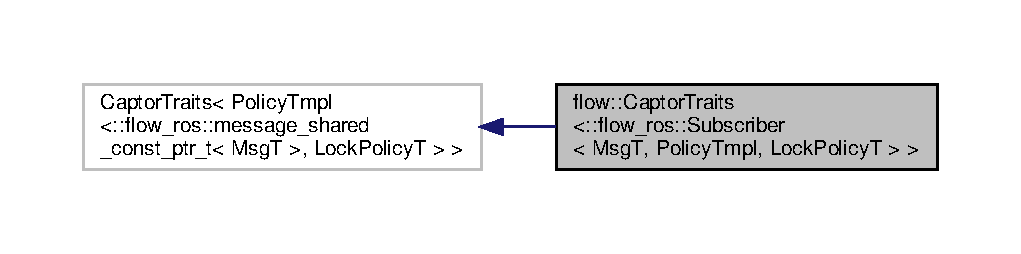
\includegraphics[width=350pt]{structflow_1_1_captor_traits_3_1_1flow__ros_1_1_subscriber_3_01_msg_t_00_01_policy_tmpl_00_01_lo021fb8bc1c700e9be0f42e0842d3e489}
\end{center}
\end{figure}


Collaboration diagram for flow\+:\+:Captor\+Traits$<$\+:\+:flow\+\_\+ros\+:\+:Subscriber$<$ MsgT, Policy\+Tmpl, Lock\+PolicyT $>$ $>$\+:\nopagebreak
\begin{figure}[H]
\begin{center}
\leavevmode
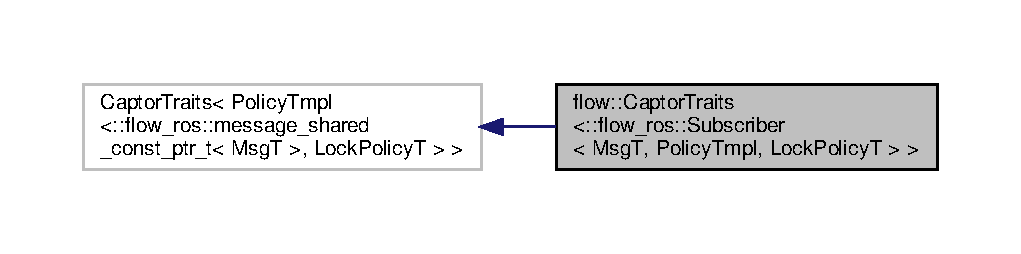
\includegraphics[width=350pt]{structflow_1_1_captor_traits_3_1_1flow__ros_1_1_subscriber_3_01_msg_t_00_01_policy_tmpl_00_01_lo6f803b65cacd3db302267201dc975f50}
\end{center}
\end{figure}


\subsection{Detailed Description}
\subsubsection*{template$<$typename MsgT, template$<$ typename... $>$ class Policy\+Tmpl, typename Lock\+PolicyT$>$\newline
struct flow\+::\+Captor\+Traits$<$\+::flow\+\_\+ros\+::\+Subscriber$<$ Msg\+T, Policy\+Tmpl, Lock\+Policy\+T $>$ $>$}

Captor traits associated with underlying Captor of Subscriber. 

The documentation for this struct was generated from the following file\+:\begin{DoxyCompactItemize}
\item 
flow\+\_\+ros/include/\hyperlink{subscriber_8h}{subscriber.\+h}\end{DoxyCompactItemize}

\hypertarget{structflow_1_1_captor_traits_3_1_1flow__ros_1_1_subscriber_policy_base_3_01_policy_t_01_4_01_4}{}\section{flow\+:\+:Captor\+Traits$<$\+:\+:flow\+\_\+ros\+:\+:Subscriber\+Policy\+Base$<$ PolicyT $>$ $>$ Struct Template Reference}
\label{structflow_1_1_captor_traits_3_1_1flow__ros_1_1_subscriber_policy_base_3_01_policy_t_01_4_01_4}\index{flow\+::\+Captor\+Traits$<$\+::flow\+\_\+ros\+::\+Subscriber\+Policy\+Base$<$ Policy\+T $>$ $>$@{flow\+::\+Captor\+Traits$<$\+::flow\+\_\+ros\+::\+Subscriber\+Policy\+Base$<$ Policy\+T $>$ $>$}}


Captor traits associated with underlying Captor of Subscriber\+Policy\+Base.  




{\ttfamily \#include $<$subscriber.\+h$>$}



Inheritance diagram for flow\+:\+:Captor\+Traits$<$\+:\+:flow\+\_\+ros\+:\+:Subscriber\+Policy\+Base$<$ PolicyT $>$ $>$\+:\nopagebreak
\begin{figure}[H]
\begin{center}
\leavevmode
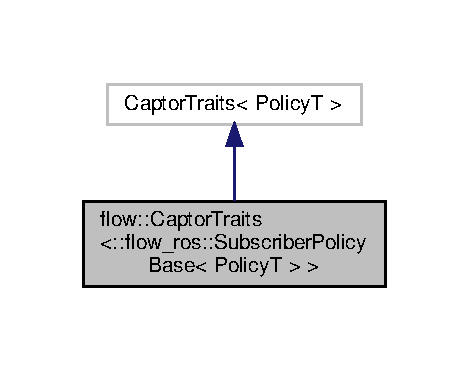
\includegraphics[width=225pt]{structflow_1_1_captor_traits_3_1_1flow__ros_1_1_subscriber_policy_base_3_01_policy_t_01_4_01_4__inherit__graph}
\end{center}
\end{figure}


Collaboration diagram for flow\+:\+:Captor\+Traits$<$\+:\+:flow\+\_\+ros\+:\+:Subscriber\+Policy\+Base$<$ PolicyT $>$ $>$\+:\nopagebreak
\begin{figure}[H]
\begin{center}
\leavevmode
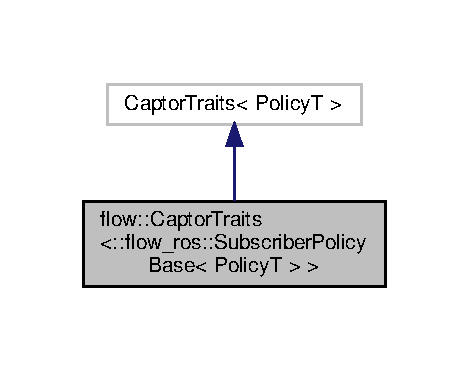
\includegraphics[width=225pt]{structflow_1_1_captor_traits_3_1_1flow__ros_1_1_subscriber_policy_base_3_01_policy_t_01_4_01_4__coll__graph}
\end{center}
\end{figure}


\subsection{Detailed Description}
\subsubsection*{template$<$typename PolicyT$>$\newline
struct flow\+::\+Captor\+Traits$<$\+::flow\+\_\+ros\+::\+Subscriber\+Policy\+Base$<$ Policy\+T $>$ $>$}

Captor traits associated with underlying Captor of Subscriber\+Policy\+Base. 

The documentation for this struct was generated from the following file\+:\begin{DoxyCompactItemize}
\item 
flow\+\_\+ros/include/\hyperlink{subscriber_8h}{subscriber.\+h}\end{DoxyCompactItemize}

\hypertarget{classflow__ros_1_1detail_1_1_collect_from_tuple}{}\section{flow\+\_\+ros\+:\+:detail\+:\+:Collect\+From\+Tuple$<$ Output\+IteratorT $>$ Class Template Reference}
\label{classflow__ros_1_1detail_1_1_collect_from_tuple}\index{flow\+\_\+ros\+::detail\+::\+Collect\+From\+Tuple$<$ Output\+Iterator\+T $>$@{flow\+\_\+ros\+::detail\+::\+Collect\+From\+Tuple$<$ Output\+Iterator\+T $>$}}


Collects objects from a tuples into an output container via iterator.  




{\ttfamily \#include $<$event\+\_\+handler.\+hpp$>$}

\subsection*{Public Member Functions}
\begin{DoxyCompactItemize}
\item 
\mbox{\Hypertarget{classflow__ros_1_1detail_1_1_collect_from_tuple_a91d23020033dc73749a5575333b8f021}\label{classflow__ros_1_1detail_1_1_collect_from_tuple_a91d23020033dc73749a5575333b8f021}} 
{\bfseries Collect\+From\+Tuple} (Output\+IteratorT output\+\_\+itr)
\item 
\mbox{\Hypertarget{classflow__ros_1_1detail_1_1_collect_from_tuple_a10e163b928e05c78f2164f99bdb3cbad}\label{classflow__ros_1_1detail_1_1_collect_from_tuple_a10e163b928e05c78f2164f99bdb3cbad}} 
{\footnotesize template$<$typename Channel\+PtrT $>$ }\\void {\bfseries operator()} (Channel\+PtrT channel)
\end{DoxyCompactItemize}


\subsection{Detailed Description}
\subsubsection*{template$<$typename Output\+IteratorT$>$\newline
class flow\+\_\+ros\+::detail\+::\+Collect\+From\+Tuple$<$ Output\+Iterator\+T $>$}

Collects objects from a tuples into an output container via iterator. 

The documentation for this class was generated from the following file\+:\begin{DoxyCompactItemize}
\item 
flow\+\_\+ros/include/impl/event\+\_\+handler.\+hpp\end{DoxyCompactItemize}

\hypertarget{structflow__ros_1_1_default_message_seq_dispatch_access}{}\section{flow\+\_\+ros\+:\+:Default\+Message\+Seq\+Dispatch\+Access Struct Reference}
\label{structflow__ros_1_1_default_message_seq_dispatch_access}\index{flow\+\_\+ros\+::\+Default\+Message\+Seq\+Dispatch\+Access@{flow\+\_\+ros\+::\+Default\+Message\+Seq\+Dispatch\+Access}}


Defines default message accessors to use a fall-\/back when defining {\ttfamily \hyperlink{structflow_1_1_dispatch_access}{flow\+::\+Dispatch\+Access}}  




{\ttfamily \#include $<$message\+\_\+seq\+\_\+access.\+h$>$}



Inheritance diagram for flow\+\_\+ros\+:\+:Default\+Message\+Seq\+Dispatch\+Access\+:\nopagebreak
\begin{figure}[H]
\begin{center}
\leavevmode
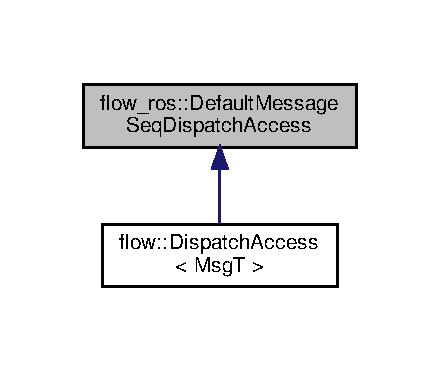
\includegraphics[width=211pt]{structflow__ros_1_1_default_message_seq_dispatch_access__inherit__graph}
\end{center}
\end{figure}
\subsection*{Static Public Member Functions}
\begin{DoxyCompactItemize}
\item 
\mbox{\Hypertarget{structflow__ros_1_1_default_message_seq_dispatch_access_afb8807ce253d3a876b4b2d8ba9046757}\label{structflow__ros_1_1_default_message_seq_dispatch_access_afb8807ce253d3a876b4b2d8ba9046757}} 
{\footnotesize template$<$typename Msg\+PtrT $>$ }\\static std\+::uint32\+\_\+t \hyperlink{structflow__ros_1_1_default_message_seq_dispatch_access_afb8807ce253d3a876b4b2d8ba9046757}{stamp} (const Msg\+PtrT \&message)
\begin{DoxyCompactList}\small\item\em Returns message stamp, assuming a {\ttfamily header.\+stamp} field exists. \end{DoxyCompactList}\item 
\mbox{\Hypertarget{structflow__ros_1_1_default_message_seq_dispatch_access_ad8c7f30400b1f554aed69e50f8533d6d}\label{structflow__ros_1_1_default_message_seq_dispatch_access_ad8c7f30400b1f554aed69e50f8533d6d}} 
{\footnotesize template$<$typename Msg\+PtrT $>$ }\\static const Msg\+PtrT \& \hyperlink{structflow__ros_1_1_default_message_seq_dispatch_access_ad8c7f30400b1f554aed69e50f8533d6d}{value} (const Msg\+PtrT \&message)
\begin{DoxyCompactList}\small\item\em Returns reference to message resource pointer (pass-\/through) \end{DoxyCompactList}\end{DoxyCompactItemize}


\subsection{Detailed Description}
Defines default message accessors to use a fall-\/back when defining {\ttfamily \hyperlink{structflow_1_1_dispatch_access}{flow\+::\+Dispatch\+Access}} 

The documentation for this struct was generated from the following file\+:\begin{DoxyCompactItemize}
\item 
flow\+\_\+ros/include/\hyperlink{message__seq__access_8h}{message\+\_\+seq\+\_\+access.\+h}\end{DoxyCompactItemize}

\hypertarget{structflow__ros_1_1_default_message_stamp_dispatch_access}{}\section{flow\+\_\+ros\+:\+:Default\+Message\+Stamp\+Dispatch\+Access Struct Reference}
\label{structflow__ros_1_1_default_message_stamp_dispatch_access}\index{flow\+\_\+ros\+::\+Default\+Message\+Stamp\+Dispatch\+Access@{flow\+\_\+ros\+::\+Default\+Message\+Stamp\+Dispatch\+Access}}


Defines default message accessors to use a fall-\/back when defining {\ttfamily \hyperlink{structflow_1_1_dispatch_access}{flow\+::\+Dispatch\+Access}}  




{\ttfamily \#include $<$message\+\_\+stamp\+\_\+access.\+h$>$}



Inheritance diagram for flow\+\_\+ros\+:\+:Default\+Message\+Stamp\+Dispatch\+Access\+:\nopagebreak
\begin{figure}[H]
\begin{center}
\leavevmode
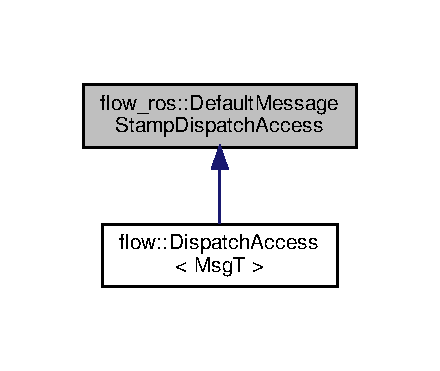
\includegraphics[width=211pt]{structflow__ros_1_1_default_message_stamp_dispatch_access__inherit__graph}
\end{center}
\end{figure}
\subsection*{Static Public Member Functions}
\begin{DoxyCompactItemize}
\item 
\mbox{\Hypertarget{structflow__ros_1_1_default_message_stamp_dispatch_access_a6884c97715e2f638e8be4fc9923f1d2d}\label{structflow__ros_1_1_default_message_stamp_dispatch_access_a6884c97715e2f638e8be4fc9923f1d2d}} 
{\footnotesize template$<$typename Msg\+PtrT $>$ }\\static const ros\+::\+Time \& \hyperlink{structflow__ros_1_1_default_message_stamp_dispatch_access_a6884c97715e2f638e8be4fc9923f1d2d}{stamp} (const Msg\+PtrT \&message)
\begin{DoxyCompactList}\small\item\em Returns message stamp, assuming a {\ttfamily header.\+stamp} field exists. \end{DoxyCompactList}\item 
\mbox{\Hypertarget{structflow__ros_1_1_default_message_stamp_dispatch_access_a476ac2553180e355327cedc97bdb302d}\label{structflow__ros_1_1_default_message_stamp_dispatch_access_a476ac2553180e355327cedc97bdb302d}} 
{\footnotesize template$<$typename Msg\+PtrT $>$ }\\static const Msg\+PtrT \& \hyperlink{structflow__ros_1_1_default_message_stamp_dispatch_access_a476ac2553180e355327cedc97bdb302d}{value} (const Msg\+PtrT \&message)
\begin{DoxyCompactList}\small\item\em Returns reference to message resource pointer (pass-\/through) \end{DoxyCompactList}\end{DoxyCompactItemize}


\subsection{Detailed Description}
Defines default message accessors to use a fall-\/back when defining {\ttfamily \hyperlink{structflow_1_1_dispatch_access}{flow\+::\+Dispatch\+Access}} 

The documentation for this struct was generated from the following file\+:\begin{DoxyCompactItemize}
\item 
flow\+\_\+ros/include/\hyperlink{message__stamp__access_8h}{message\+\_\+stamp\+\_\+access.\+h}\end{DoxyCompactItemize}

\hypertarget{structflow__ros_1_1_default_output_container_type_info}{}\section{flow\+\_\+ros\+:\+:Default\+Output\+Container\+Type\+Info$<$ DispatchT $>$ Struct Template Reference}
\label{structflow__ros_1_1_default_output_container_type_info}\index{flow\+\_\+ros\+::\+Default\+Output\+Container\+Type\+Info$<$ Dispatch\+T $>$@{flow\+\_\+ros\+::\+Default\+Output\+Container\+Type\+Info$<$ Dispatch\+T $>$}}


Default dispatch container type information.  




{\ttfamily \#include $<$event\+\_\+handler.\+h$>$}

\subsection*{Public Types}
\begin{DoxyCompactItemize}
\item 
\mbox{\Hypertarget{structflow__ros_1_1_default_output_container_type_info_a4ffbb4d1e03977b064edda2072187299}\label{structflow__ros_1_1_default_output_container_type_info_a4ffbb4d1e03977b064edda2072187299}} 
using \hyperlink{structflow__ros_1_1_default_output_container_type_info_a4ffbb4d1e03977b064edda2072187299}{Container} = std\+::vector$<$ DispatchT, std\+::allocator$<$ DispatchT $>$ $>$
\begin{DoxyCompactList}\small\item\em Output container type. \end{DoxyCompactList}\item 
\mbox{\Hypertarget{structflow__ros_1_1_default_output_container_type_info_a8fcd2ae4f8d0f4fb411b6a433b40d5f2}\label{structflow__ros_1_1_default_output_container_type_info_a8fcd2ae4f8d0f4fb411b6a433b40d5f2}} 
using \hyperlink{structflow__ros_1_1_default_output_container_type_info_a8fcd2ae4f8d0f4fb411b6a433b40d5f2}{output\+\_\+iterator\+\_\+type} = std\+::back\+\_\+insert\+\_\+iterator$<$ \hyperlink{structflow__ros_1_1_default_output_container_type_info_a4ffbb4d1e03977b064edda2072187299}{Container} $>$
\begin{DoxyCompactList}\small\item\em Container output iterator type. \end{DoxyCompactList}\end{DoxyCompactItemize}
\subsection*{Static Public Member Functions}
\begin{DoxyCompactItemize}
\item 
\mbox{\Hypertarget{structflow__ros_1_1_default_output_container_type_info_ab175492907ef77b1f512a8acaa208260}\label{structflow__ros_1_1_default_output_container_type_info_ab175492907ef77b1f512a8acaa208260}} 
static \hyperlink{structflow__ros_1_1_default_output_container_type_info_a8fcd2ae4f8d0f4fb411b6a433b40d5f2}{output\+\_\+iterator\+\_\+type} \hyperlink{structflow__ros_1_1_default_output_container_type_info_ab175492907ef77b1f512a8acaa208260}{get\+\_\+output\+\_\+iterator} (\hyperlink{structflow__ros_1_1_default_output_container_type_info_a4ffbb4d1e03977b064edda2072187299}{Container} \&c)
\begin{DoxyCompactList}\small\item\em Returns an appropriate container output iterator. \end{DoxyCompactList}\end{DoxyCompactItemize}


\subsection{Detailed Description}
\subsubsection*{template$<$typename DispatchT$>$\newline
struct flow\+\_\+ros\+::\+Default\+Output\+Container\+Type\+Info$<$ Dispatch\+T $>$}

Default dispatch container type information. 

Dispatch object collected on sync are stored into a {\ttfamily std\+::vector}


\begin{DoxyTemplParams}{Template Parameters}
{\em DispatchT} & message dispatch type \\
\hline
\end{DoxyTemplParams}


The documentation for this struct was generated from the following file\+:\begin{DoxyCompactItemize}
\item 
flow\+\_\+ros/include/\hyperlink{event__handler_8h}{event\+\_\+handler.\+h}\end{DoxyCompactItemize}

\hypertarget{structflow_1_1_dispatch_access}{}\section{flow\+:\+:Dispatch\+Access$<$ MsgT $>$ Struct Template Reference}
\label{structflow_1_1_dispatch_access}\index{flow\+::\+Dispatch\+Access$<$ Msg\+T $>$@{flow\+::\+Dispatch\+Access$<$ Msg\+T $>$}}


Template which basic methods for Message\+Dispatch.  




{\ttfamily \#include $<$message\+\_\+seq\+\_\+access.\+h$>$}



Inheritance diagram for flow\+:\+:Dispatch\+Access$<$ MsgT $>$\+:\nopagebreak
\begin{figure}[H]
\begin{center}
\leavevmode
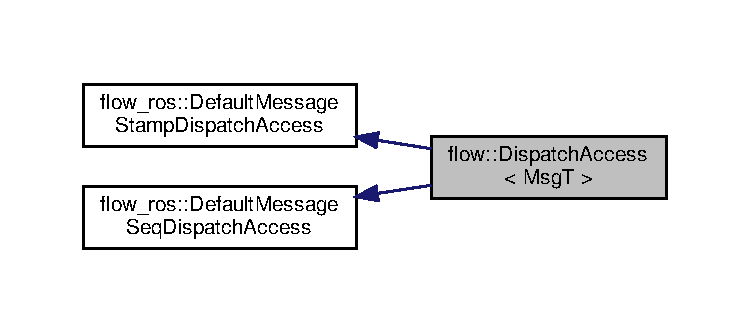
\includegraphics[width=350pt]{structflow_1_1_dispatch_access__inherit__graph}
\end{center}
\end{figure}


Collaboration diagram for flow\+:\+:Dispatch\+Access$<$ MsgT $>$\+:\nopagebreak
\begin{figure}[H]
\begin{center}
\leavevmode
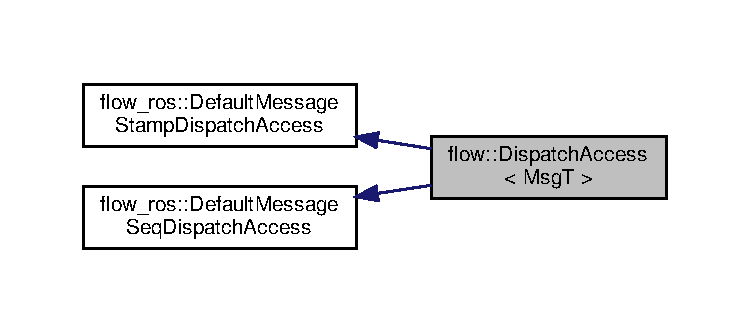
\includegraphics[width=350pt]{structflow_1_1_dispatch_access__coll__graph}
\end{center}
\end{figure}
\subsection*{Additional Inherited Members}


\subsection{Detailed Description}
\subsubsection*{template$<$typename MsgT$>$\newline
struct flow\+::\+Dispatch\+Access$<$ Msg\+T $>$}

Template which basic methods for Message\+Dispatch. 


\begin{DoxyTemplParams}{Template Parameters}
{\em MsgT} & message type \\
\hline
\end{DoxyTemplParams}


The documentation for this struct was generated from the following file\+:\begin{DoxyCompactItemize}
\item 
flow\+\_\+ros/include/\hyperlink{message__seq__access_8h}{message\+\_\+seq\+\_\+access.\+h}\end{DoxyCompactItemize}

\hypertarget{structflow_1_1_dispatch_traits_3_01boost_1_1shared__ptr_3_01const_01_msg_t_01_4_01_4}{}\section{flow\+:\+:Dispatch\+Traits$<$ boost\+:\+:shared\+\_\+ptr$<$ const MsgT $>$ $>$ Struct Template Reference}
\label{structflow_1_1_dispatch_traits_3_01boost_1_1shared__ptr_3_01const_01_msg_t_01_4_01_4}\index{flow\+::\+Dispatch\+Traits$<$ boost\+::shared\+\_\+ptr$<$ const Msg\+T $>$ $>$@{flow\+::\+Dispatch\+Traits$<$ boost\+::shared\+\_\+ptr$<$ const Msg\+T $>$ $>$}}


Default R\+OS message Dispatch traits.  




{\ttfamily \#include $<$message\+\_\+seq\+\_\+access.\+h$>$}

\subsection*{Public Types}
\begin{DoxyCompactItemize}
\item 
\mbox{\Hypertarget{structflow_1_1_dispatch_traits_3_01boost_1_1shared__ptr_3_01const_01_msg_t_01_4_01_4_ac273b96fb741fccc6e59755dfd3c6e41}\label{structflow_1_1_dispatch_traits_3_01boost_1_1shared__ptr_3_01const_01_msg_t_01_4_01_4_ac273b96fb741fccc6e59755dfd3c6e41}} 
using \hyperlink{structflow_1_1_dispatch_traits_3_01boost_1_1shared__ptr_3_01const_01_msg_t_01_4_01_4_ac273b96fb741fccc6e59755dfd3c6e41}{stamp\+\_\+type} = std\+::uint32\+\_\+t
\begin{DoxyCompactList}\small\item\em Dispatch stamp type. \end{DoxyCompactList}\item 
\mbox{\Hypertarget{structflow_1_1_dispatch_traits_3_01boost_1_1shared__ptr_3_01const_01_msg_t_01_4_01_4_aa17069d8567e8bd05ac5ebced3b190c1}\label{structflow_1_1_dispatch_traits_3_01boost_1_1shared__ptr_3_01const_01_msg_t_01_4_01_4_aa17069d8567e8bd05ac5ebced3b190c1}} 
using \hyperlink{structflow_1_1_dispatch_traits_3_01boost_1_1shared__ptr_3_01const_01_msg_t_01_4_01_4_aa17069d8567e8bd05ac5ebced3b190c1}{value\+\_\+type} = boost\+::shared\+\_\+ptr$<$ const MsgT $>$
\begin{DoxyCompactList}\small\item\em Dispatch data type. \end{DoxyCompactList}\item 
\mbox{\Hypertarget{structflow_1_1_dispatch_traits_3_01boost_1_1shared__ptr_3_01const_01_msg_t_01_4_01_4_a053ced6a59b8de426b826b910167d7af}\label{structflow_1_1_dispatch_traits_3_01boost_1_1shared__ptr_3_01const_01_msg_t_01_4_01_4_a053ced6a59b8de426b826b910167d7af}} 
using \hyperlink{structflow_1_1_dispatch_traits_3_01boost_1_1shared__ptr_3_01const_01_msg_t_01_4_01_4_a053ced6a59b8de426b826b910167d7af}{stamp\+\_\+type} = ros\+::\+Time
\begin{DoxyCompactList}\small\item\em Dispatch stamp type. \end{DoxyCompactList}\item 
\mbox{\Hypertarget{structflow_1_1_dispatch_traits_3_01boost_1_1shared__ptr_3_01const_01_msg_t_01_4_01_4_aa17069d8567e8bd05ac5ebced3b190c1}\label{structflow_1_1_dispatch_traits_3_01boost_1_1shared__ptr_3_01const_01_msg_t_01_4_01_4_aa17069d8567e8bd05ac5ebced3b190c1}} 
using \hyperlink{structflow_1_1_dispatch_traits_3_01boost_1_1shared__ptr_3_01const_01_msg_t_01_4_01_4_aa17069d8567e8bd05ac5ebced3b190c1}{value\+\_\+type} = boost\+::shared\+\_\+ptr$<$ const MsgT $>$
\begin{DoxyCompactList}\small\item\em Dispatch data type. \end{DoxyCompactList}\end{DoxyCompactItemize}


\subsection{Detailed Description}
\subsubsection*{template$<$typename MsgT$>$\newline
struct flow\+::\+Dispatch\+Traits$<$ boost\+::shared\+\_\+ptr$<$ const Msg\+T $>$ $>$}

Default R\+OS message Dispatch traits. 

The documentation for this struct was generated from the following files\+:\begin{DoxyCompactItemize}
\item 
flow\+\_\+ros/include/\hyperlink{message__seq__access_8h}{message\+\_\+seq\+\_\+access.\+h}\item 
flow\+\_\+ros/include/\hyperlink{message__stamp__access_8h}{message\+\_\+stamp\+\_\+access.\+h}\end{DoxyCompactItemize}

\hypertarget{structflow_1_1_dispatch_traits_3_01std_1_1shared__ptr_3_01const_01_msg_t_01_4_01_4}{}\section{flow\+:\+:Dispatch\+Traits$<$ std\+:\+:shared\+\_\+ptr$<$ const MsgT $>$ $>$ Struct Template Reference}
\label{structflow_1_1_dispatch_traits_3_01std_1_1shared__ptr_3_01const_01_msg_t_01_4_01_4}\index{flow\+::\+Dispatch\+Traits$<$ std\+::shared\+\_\+ptr$<$ const Msg\+T $>$ $>$@{flow\+::\+Dispatch\+Traits$<$ std\+::shared\+\_\+ptr$<$ const Msg\+T $>$ $>$}}


Default R\+OS message-\/like Dispatch traits.  




{\ttfamily \#include $<$message\+\_\+seq\+\_\+access.\+h$>$}

\subsection*{Public Types}
\begin{DoxyCompactItemize}
\item 
\mbox{\Hypertarget{structflow_1_1_dispatch_traits_3_01std_1_1shared__ptr_3_01const_01_msg_t_01_4_01_4_a30c24c96f30de78bafe10490d72ae489}\label{structflow_1_1_dispatch_traits_3_01std_1_1shared__ptr_3_01const_01_msg_t_01_4_01_4_a30c24c96f30de78bafe10490d72ae489}} 
using \hyperlink{structflow_1_1_dispatch_traits_3_01std_1_1shared__ptr_3_01const_01_msg_t_01_4_01_4_a30c24c96f30de78bafe10490d72ae489}{stamp\+\_\+type} = std\+::uint32\+\_\+t
\begin{DoxyCompactList}\small\item\em Dispatch stamp type. \end{DoxyCompactList}\item 
\mbox{\Hypertarget{structflow_1_1_dispatch_traits_3_01std_1_1shared__ptr_3_01const_01_msg_t_01_4_01_4_a9a75b524c93967f62932e6e9631067fa}\label{structflow_1_1_dispatch_traits_3_01std_1_1shared__ptr_3_01const_01_msg_t_01_4_01_4_a9a75b524c93967f62932e6e9631067fa}} 
using \hyperlink{structflow_1_1_dispatch_traits_3_01std_1_1shared__ptr_3_01const_01_msg_t_01_4_01_4_a9a75b524c93967f62932e6e9631067fa}{value\+\_\+type} = std\+::shared\+\_\+ptr$<$ const MsgT $>$
\begin{DoxyCompactList}\small\item\em Dispatch data type. \end{DoxyCompactList}\item 
\mbox{\Hypertarget{structflow_1_1_dispatch_traits_3_01std_1_1shared__ptr_3_01const_01_msg_t_01_4_01_4_ace1068fadd4b54817d87e452955c6484}\label{structflow_1_1_dispatch_traits_3_01std_1_1shared__ptr_3_01const_01_msg_t_01_4_01_4_ace1068fadd4b54817d87e452955c6484}} 
using \hyperlink{structflow_1_1_dispatch_traits_3_01std_1_1shared__ptr_3_01const_01_msg_t_01_4_01_4_ace1068fadd4b54817d87e452955c6484}{stamp\+\_\+type} = ros\+::\+Time
\begin{DoxyCompactList}\small\item\em Dispatch stamp type. \end{DoxyCompactList}\item 
\mbox{\Hypertarget{structflow_1_1_dispatch_traits_3_01std_1_1shared__ptr_3_01const_01_msg_t_01_4_01_4_a9a75b524c93967f62932e6e9631067fa}\label{structflow_1_1_dispatch_traits_3_01std_1_1shared__ptr_3_01const_01_msg_t_01_4_01_4_a9a75b524c93967f62932e6e9631067fa}} 
using \hyperlink{structflow_1_1_dispatch_traits_3_01std_1_1shared__ptr_3_01const_01_msg_t_01_4_01_4_a9a75b524c93967f62932e6e9631067fa}{value\+\_\+type} = std\+::shared\+\_\+ptr$<$ const MsgT $>$
\begin{DoxyCompactList}\small\item\em Dispatch data type. \end{DoxyCompactList}\end{DoxyCompactItemize}


\subsection{Detailed Description}
\subsubsection*{template$<$typename MsgT$>$\newline
struct flow\+::\+Dispatch\+Traits$<$ std\+::shared\+\_\+ptr$<$ const Msg\+T $>$ $>$}

Default R\+OS message-\/like Dispatch traits. 

The documentation for this struct was generated from the following files\+:\begin{DoxyCompactItemize}
\item 
flow\+\_\+ros/include/\hyperlink{message__seq__access_8h}{message\+\_\+seq\+\_\+access.\+h}\item 
flow\+\_\+ros/include/\hyperlink{message__stamp__access_8h}{message\+\_\+stamp\+\_\+access.\+h}\end{DoxyCompactItemize}

\hypertarget{classflow__ros_1_1_event_handler}{}\section{flow\+\_\+ros\+:\+:Event\+Handler$<$ Publisher\+Tuple, Subscriber\+Tuple, Output\+Container\+Type\+Info\+Tmpl $>$ Class Template Reference}
\label{classflow__ros_1_1_event_handler}\index{flow\+\_\+ros\+::\+Event\+Handler$<$ Publisher\+Tuple, Subscriber\+Tuple, Output\+Container\+Type\+Info\+Tmpl $>$@{flow\+\_\+ros\+::\+Event\+Handler$<$ Publisher\+Tuple, Subscriber\+Tuple, Output\+Container\+Type\+Info\+Tmpl $>$}}


Manages a input and output channels, and runs callbacks on input synchronization.  




{\ttfamily \#include $<$event\+\_\+handler.\+h$>$}



Inheritance diagram for flow\+\_\+ros\+:\+:Event\+Handler$<$ Publisher\+Tuple, Subscriber\+Tuple, Output\+Container\+Type\+Info\+Tmpl $>$\+:\nopagebreak
\begin{figure}[H]
\begin{center}
\leavevmode
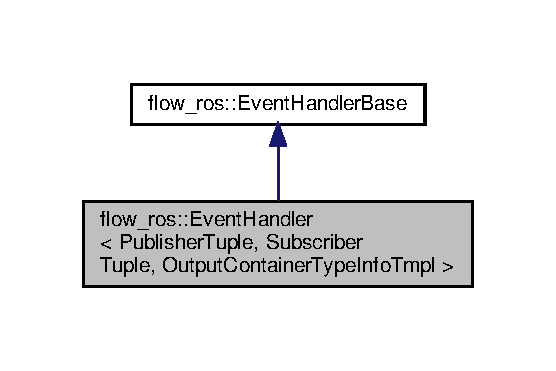
\includegraphics[width=267pt]{classflow__ros_1_1_event_handler__inherit__graph}
\end{center}
\end{figure}


Collaboration diagram for flow\+\_\+ros\+:\+:Event\+Handler$<$ Publisher\+Tuple, Subscriber\+Tuple, Output\+Container\+Type\+Info\+Tmpl $>$\+:\nopagebreak
\begin{figure}[H]
\begin{center}
\leavevmode
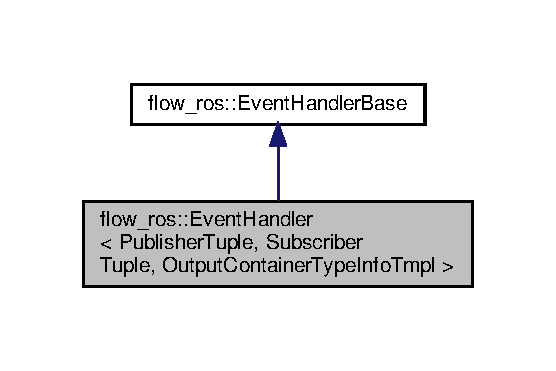
\includegraphics[width=267pt]{classflow__ros_1_1_event_handler__coll__graph}
\end{center}
\end{figure}
\subsection*{Classes}
\begin{DoxyCompactItemize}
\item 
struct \hyperlink{structflow__ros_1_1_event_handler_1_1_callbacks}{Callbacks}
\begin{DoxyCompactList}\small\item\em \hyperlink{classflow__ros_1_1_event_handler}{Event\+Handler} callback options. \end{DoxyCompactList}\end{DoxyCompactItemize}
\subsection*{Public Types}
\begin{DoxyCompactItemize}
\item 
\mbox{\Hypertarget{classflow__ros_1_1_event_handler_aced903010cf36b1ce0d9bceb0f7ac64a}\label{classflow__ros_1_1_event_handler_aced903010cf36b1ce0d9bceb0f7ac64a}} 
using \hyperlink{classflow__ros_1_1_event_handler_aced903010cf36b1ce0d9bceb0f7ac64a}{Publisher\+Ptr\+Tuple} = typename \hyperlink{structflow__ros_1_1detail_1_1_wrap_tuple_elements}{detail\+::\+Wrap\+Tuple\+Elements}$<$ std\+::shared\+\_\+ptr, Publisher\+Tuple $>$\+::type
\begin{DoxyCompactList}\small\item\em Tuple of publisher resource pointers. \end{DoxyCompactList}\item 
\mbox{\Hypertarget{classflow__ros_1_1_event_handler_a5c37a3eace3da99b2068cfa1fd34449a}\label{classflow__ros_1_1_event_handler_a5c37a3eace3da99b2068cfa1fd34449a}} 
using \hyperlink{classflow__ros_1_1_event_handler_a5c37a3eace3da99b2068cfa1fd34449a}{Subscriber\+Ptr\+Tuple} = typename \hyperlink{structflow__ros_1_1detail_1_1_wrap_tuple_elements}{detail\+::\+Wrap\+Tuple\+Elements}$<$ std\+::shared\+\_\+ptr, Subscriber\+Tuple $>$\+::type
\begin{DoxyCompactList}\small\item\em Tuple of subscriber resource pointers. \end{DoxyCompactList}\item 
using \hyperlink{classflow__ros_1_1_event_handler_ae5dc263e5c12a4b7fb60f320dc403173}{Output} = typename \hyperlink{structflow__ros_1_1detail_1_1_event_handler_output_type}{detail\+::\+Event\+Handler\+Output\+Type}$<$ Publisher\+Tuple $>$\+::type
\begin{DoxyCompactList}\small\item\em Output data type. \end{DoxyCompactList}\item 
using \hyperlink{classflow__ros_1_1_event_handler_a53af7756aaf98646281d57b036510d56}{Input} = typename \hyperlink{structflow__ros_1_1detail_1_1_event_handler_input_type}{detail\+::\+Event\+Handler\+Input\+Type}$<$ Output\+Container\+Type\+Info\+Tmpl, Subscriber\+Tuple $>$\+::type
\begin{DoxyCompactList}\small\item\em Synchronized input container type. \end{DoxyCompactList}\end{DoxyCompactItemize}
\subsection*{Public Member Functions}
\begin{DoxyCompactItemize}
\item 
\hyperlink{classflow__ros_1_1_event_handler_a24c8067f4faeef500cd4475b6cdfc33e}{Event\+Handler} (\hyperlink{structflow__ros_1_1_event_handler_1_1_callbacks}{Callbacks} callbacks, \hyperlink{classflow__ros_1_1_event_handler_aced903010cf36b1ce0d9bceb0f7ac64a}{Publisher\+Ptr\+Tuple} publishers, \hyperlink{classflow__ros_1_1_event_handler_a5c37a3eace3da99b2068cfa1fd34449a}{Subscriber\+Ptr\+Tuple} subscribers)
\begin{DoxyCompactList}\small\item\em Required setup constructor. \end{DoxyCompactList}\item 
\mbox{\Hypertarget{classflow__ros_1_1_event_handler_ae8f5d3a668f27b165cb2702513a9f447}\label{classflow__ros_1_1_event_handler_ae8f5d3a668f27b165cb2702513a9f447}} 
\hyperlink{classflow__ros_1_1_event_handler_ae8f5d3a668f27b165cb2702513a9f447}{$\sim$\+Event\+Handler} ()=default
\begin{DoxyCompactList}\small\item\em Destructor. \end{DoxyCompactList}\item 
\hyperlink{structflow__ros_1_1_event_summary}{Event\+Summary} \hyperlink{classflow__ros_1_1_event_handler_abc2f1821d85ab05d86270cbf20da6cd9}{dry\+\_\+update} () override
\item 
\hyperlink{structflow__ros_1_1_event_summary}{Event\+Summary} \hyperlink{classflow__ros_1_1_event_handler_a445ecc20268a455bf47df8598413ae67}{update} (const std\+::chrono\+::steady\+\_\+clock\+::time\+\_\+point timeout=std\+::chrono\+::steady\+\_\+clock\+::time\+\_\+point\+::max()) override
\begin{DoxyCompactList}\small\item\em Event updater method. \end{DoxyCompactList}\item 
void \hyperlink{classflow__ros_1_1_event_handler_aeaf45592fd8c7fe8c3a4b0da23496d69}{remove} (const ros\+::\+Time \&t\+\_\+remove) override
\begin{DoxyCompactList}\small\item\em Removes all events before specified time. \end{DoxyCompactList}\item 
void \hyperlink{classflow__ros_1_1_event_handler_a95200a36fc64725ac280c04c2697f709}{abort} (const ros\+::\+Time \&t\+\_\+abort) override
\begin{DoxyCompactList}\small\item\em Aborts all event at or before specified time. \end{DoxyCompactList}\item 
void \hyperlink{classflow__ros_1_1_event_handler_a4b9b96163817d60208a83476148562ff}{reset} () override
\begin{DoxyCompactList}\small\item\em Resets event handler and all managed channels. \end{DoxyCompactList}\item 
std\+::vector$<$ std\+::shared\+\_\+ptr$<$ const \hyperlink{classflow__ros_1_1_subscriber_base}{Subscriber\+Base} $>$ $>$ \hyperlink{classflow__ros_1_1_event_handler_ac91cf67be38d79d3d86a9aa6318eca53}{get\+Subscribers} () const override
\begin{DoxyCompactList}\small\item\em Returns vector of subscriber resources associated with \hyperlink{classflow__ros_1_1_event_handler}{Event\+Handler}. \end{DoxyCompactList}\item 
std\+::vector$<$ std\+::shared\+\_\+ptr$<$ const \hyperlink{classflow__ros_1_1_publisher_base}{Publisher\+Base} $>$ $>$ \hyperlink{classflow__ros_1_1_event_handler_ae786846cf4cf48b9b952265862e73ef1}{get\+Publishers} () const override
\begin{DoxyCompactList}\small\item\em Returns vector of publisher resources associated with \hyperlink{classflow__ros_1_1_event_handler}{Event\+Handler}. \end{DoxyCompactList}\end{DoxyCompactItemize}


\subsection{Detailed Description}
\subsubsection*{template$<$typename Publisher\+Tuple, typename Subscriber\+Tuple, template$<$ typename $>$ class Output\+Container\+Type\+Info\+Tmpl = Default\+Output\+Container\+Type\+Info$>$\newline
class flow\+\_\+ros\+::\+Event\+Handler$<$ Publisher\+Tuple, Subscriber\+Tuple, Output\+Container\+Type\+Info\+Tmpl $>$}

Manages a input and output channels, and runs callbacks on input synchronization. 


\begin{DoxyTemplParams}{Template Parameters}
{\em Publisher\+Tuple} & tuple of publisher types \\
\hline
{\em Subscriber\+Tuple} & tuple of subscriber types \\
\hline
{\em Dispatch\+ContainerT} & a container type description class; specifies what type of container to use when \& capturing messages, and how to fill that container using an output iterator \\
\hline
\end{DoxyTemplParams}


\subsection{Member Typedef Documentation}
\mbox{\Hypertarget{classflow__ros_1_1_event_handler_a53af7756aaf98646281d57b036510d56}\label{classflow__ros_1_1_event_handler_a53af7756aaf98646281d57b036510d56}} 
\index{flow\+\_\+ros\+::\+Event\+Handler@{flow\+\_\+ros\+::\+Event\+Handler}!Input@{Input}}
\index{Input@{Input}!flow\+\_\+ros\+::\+Event\+Handler@{flow\+\_\+ros\+::\+Event\+Handler}}
\subsubsection{\texorpdfstring{Input}{Input}}
{\footnotesize\ttfamily template$<$typename Publisher\+Tuple , typename Subscriber\+Tuple , template$<$ typename $>$ class Output\+Container\+Type\+Info\+Tmpl = Default\+Output\+Container\+Type\+Info$>$ \\
using \hyperlink{classflow__ros_1_1_event_handler}{flow\+\_\+ros\+::\+Event\+Handler}$<$ Publisher\+Tuple, Subscriber\+Tuple, Output\+Container\+Type\+Info\+Tmpl $>$\+::\hyperlink{classflow__ros_1_1_event_handler_a53af7756aaf98646281d57b036510d56}{Input} =  typename \hyperlink{structflow__ros_1_1detail_1_1_event_handler_input_type}{detail\+::\+Event\+Handler\+Input\+Type}$<$Output\+Container\+Type\+Info\+Tmpl, Subscriber\+Tuple$>$\+::type}



Synchronized input container type. 

{\ttfamily std\+::tuple$<$...$>$} with data from each synchronized input. Inputs are ordered with respect to the ordering of the capture buffers from which they were sources, specified by {\ttfamily Subscriber\+Tuple} \mbox{\Hypertarget{classflow__ros_1_1_event_handler_ae5dc263e5c12a4b7fb60f320dc403173}\label{classflow__ros_1_1_event_handler_ae5dc263e5c12a4b7fb60f320dc403173}} 
\index{flow\+\_\+ros\+::\+Event\+Handler@{flow\+\_\+ros\+::\+Event\+Handler}!Output@{Output}}
\index{Output@{Output}!flow\+\_\+ros\+::\+Event\+Handler@{flow\+\_\+ros\+::\+Event\+Handler}}
\subsubsection{\texorpdfstring{Output}{Output}}
{\footnotesize\ttfamily template$<$typename Publisher\+Tuple , typename Subscriber\+Tuple , template$<$ typename $>$ class Output\+Container\+Type\+Info\+Tmpl = Default\+Output\+Container\+Type\+Info$>$ \\
using \hyperlink{classflow__ros_1_1_event_handler}{flow\+\_\+ros\+::\+Event\+Handler}$<$ Publisher\+Tuple, Subscriber\+Tuple, Output\+Container\+Type\+Info\+Tmpl $>$\+::\hyperlink{classflow__ros_1_1_event_handler_ae5dc263e5c12a4b7fb60f320dc403173}{Output} =  typename \hyperlink{structflow__ros_1_1detail_1_1_event_handler_output_type}{detail\+::\+Event\+Handler\+Output\+Type}$<$Publisher\+Tuple$>$\+::type}



Output data type. 

Message type returned from event callback. If\+:
\begin{DoxyItemize}
\item {\ttfamily Publisher\+Tuple} specifies a single output, then this is a {\ttfamily Output\+Msg\+T\+::\+Ptr} associated with that publisher
\end{DoxyItemize}

{\ttfamily Publisher\+Tuple} specifies multiple outputs, then this is a {\ttfamily std\+::tuple$<$\+Output0\+Msg\+T\+::\+Ptr, ... , Output\+N\+Msg\+T\+::\+Ptr$>$} associated with those publishers in the order specified by {\ttfamily Publisher\+Tuple}. 

\subsection{Constructor \& Destructor Documentation}
\mbox{\Hypertarget{classflow__ros_1_1_event_handler_a24c8067f4faeef500cd4475b6cdfc33e}\label{classflow__ros_1_1_event_handler_a24c8067f4faeef500cd4475b6cdfc33e}} 
\index{flow\+\_\+ros\+::\+Event\+Handler@{flow\+\_\+ros\+::\+Event\+Handler}!Event\+Handler@{Event\+Handler}}
\index{Event\+Handler@{Event\+Handler}!flow\+\_\+ros\+::\+Event\+Handler@{flow\+\_\+ros\+::\+Event\+Handler}}
\subsubsection{\texorpdfstring{Event\+Handler()}{EventHandler()}}
{\footnotesize\ttfamily template$<$typename Publisher\+Tuple , typename Subscriber\+Tuple , template$<$ typename $>$ class Output\+Container\+Type\+Info\+Tmpl = Default\+Output\+Container\+Type\+Info$>$ \\
\hyperlink{classflow__ros_1_1_event_handler}{flow\+\_\+ros\+::\+Event\+Handler}$<$ Publisher\+Tuple, Subscriber\+Tuple, Output\+Container\+Type\+Info\+Tmpl $>$\+::\hyperlink{classflow__ros_1_1_event_handler}{Event\+Handler} (\begin{DoxyParamCaption}\item[{\hyperlink{structflow__ros_1_1_event_handler_1_1_callbacks}{Callbacks}}]{callbacks,  }\item[{\hyperlink{classflow__ros_1_1_event_handler_aced903010cf36b1ce0d9bceb0f7ac64a}{Publisher\+Ptr\+Tuple}}]{publishers,  }\item[{\hyperlink{classflow__ros_1_1_event_handler_a5c37a3eace3da99b2068cfa1fd34449a}{Subscriber\+Ptr\+Tuple}}]{subscribers }\end{DoxyParamCaption})\hspace{0.3cm}{\ttfamily [inline]}}



Required setup constructor. 


\begin{DoxyParams}{Parameters}
{\em callbacks} & callback to run after input synchronization \\
\hline
{\em publishers} & message output channel resources \\
\hline
{\em subscribers} & message input channel resources \\
\hline
\end{DoxyParams}


\subsection{Member Function Documentation}
\mbox{\Hypertarget{classflow__ros_1_1_event_handler_a95200a36fc64725ac280c04c2697f709}\label{classflow__ros_1_1_event_handler_a95200a36fc64725ac280c04c2697f709}} 
\index{flow\+\_\+ros\+::\+Event\+Handler@{flow\+\_\+ros\+::\+Event\+Handler}!abort@{abort}}
\index{abort@{abort}!flow\+\_\+ros\+::\+Event\+Handler@{flow\+\_\+ros\+::\+Event\+Handler}}
\subsubsection{\texorpdfstring{abort()}{abort()}}
{\footnotesize\ttfamily template$<$typename Publisher\+Tuple , typename Subscriber\+Tuple , template$<$ typename $>$ class Output\+Container\+Type\+Info\+Tmpl = Default\+Output\+Container\+Type\+Info$>$ \\
void \hyperlink{classflow__ros_1_1_event_handler}{flow\+\_\+ros\+::\+Event\+Handler}$<$ Publisher\+Tuple, Subscriber\+Tuple, Output\+Container\+Type\+Info\+Tmpl $>$\+::abort (\begin{DoxyParamCaption}\item[{const ros\+::\+Time \&}]{t\+\_\+abort }\end{DoxyParamCaption})\hspace{0.3cm}{\ttfamily [inline]}, {\ttfamily [override]}, {\ttfamily [virtual]}}



Aborts all event at or before specified time. 


\begin{DoxyParams}{Parameters}
{\em t\+\_\+abort} & time before which events should be aborted \\
\hline
\end{DoxyParams}


Implements \hyperlink{classflow__ros_1_1_event_handler_base_a5611152cffdc62a4215726d19ce58ab5}{flow\+\_\+ros\+::\+Event\+Handler\+Base}.

\mbox{\Hypertarget{classflow__ros_1_1_event_handler_abc2f1821d85ab05d86270cbf20da6cd9}\label{classflow__ros_1_1_event_handler_abc2f1821d85ab05d86270cbf20da6cd9}} 
\index{flow\+\_\+ros\+::\+Event\+Handler@{flow\+\_\+ros\+::\+Event\+Handler}!dry\+\_\+update@{dry\+\_\+update}}
\index{dry\+\_\+update@{dry\+\_\+update}!flow\+\_\+ros\+::\+Event\+Handler@{flow\+\_\+ros\+::\+Event\+Handler}}
\subsubsection{\texorpdfstring{dry\+\_\+update()}{dry\_update()}}
{\footnotesize\ttfamily template$<$typename Publisher\+Tuple , typename Subscriber\+Tuple , template$<$ typename $>$ class Output\+Container\+Type\+Info\+Tmpl = Default\+Output\+Container\+Type\+Info$>$ \\
\hyperlink{structflow__ros_1_1_event_summary}{Event\+Summary} \hyperlink{classflow__ros_1_1_event_handler}{flow\+\_\+ros\+::\+Event\+Handler}$<$ Publisher\+Tuple, Subscriber\+Tuple, Output\+Container\+Type\+Info\+Tmpl $>$\+::dry\+\_\+update (\begin{DoxyParamCaption}{ }\end{DoxyParamCaption})\hspace{0.3cm}{\ttfamily [inline]}, {\ttfamily [override]}, {\ttfamily [virtual]}}







Implements \hyperlink{classflow__ros_1_1_event_handler_base_a85873d1e3eaa3c152295c5c49d5948f6}{flow\+\_\+ros\+::\+Event\+Handler\+Base}.

\mbox{\Hypertarget{classflow__ros_1_1_event_handler_ae786846cf4cf48b9b952265862e73ef1}\label{classflow__ros_1_1_event_handler_ae786846cf4cf48b9b952265862e73ef1}} 
\index{flow\+\_\+ros\+::\+Event\+Handler@{flow\+\_\+ros\+::\+Event\+Handler}!get\+Publishers@{get\+Publishers}}
\index{get\+Publishers@{get\+Publishers}!flow\+\_\+ros\+::\+Event\+Handler@{flow\+\_\+ros\+::\+Event\+Handler}}
\subsubsection{\texorpdfstring{get\+Publishers()}{getPublishers()}}
{\footnotesize\ttfamily template$<$typename Publisher\+Tuple , typename Subscriber\+Tuple , template$<$ typename $>$ class Output\+Container\+Type\+Info\+Tmpl = Default\+Output\+Container\+Type\+Info$>$ \\
std\+::vector$<$std\+::shared\+\_\+ptr$<$const \hyperlink{classflow__ros_1_1_publisher_base}{Publisher\+Base}$>$ $>$ \hyperlink{classflow__ros_1_1_event_handler}{flow\+\_\+ros\+::\+Event\+Handler}$<$ Publisher\+Tuple, Subscriber\+Tuple, Output\+Container\+Type\+Info\+Tmpl $>$\+::get\+Publishers (\begin{DoxyParamCaption}{ }\end{DoxyParamCaption}) const\hspace{0.3cm}{\ttfamily [inline]}, {\ttfamily [override]}, {\ttfamily [virtual]}}



Returns vector of publisher resources associated with \hyperlink{classflow__ros_1_1_event_handler}{Event\+Handler}. 

\begin{DoxyNote}{Note}
Resource pointers in return value provide partial access to meta information about \hyperlink{classflow__ros_1_1_publisher}{Publisher} objects, but do not allow for data mutation 
\end{DoxyNote}


Implements \hyperlink{classflow__ros_1_1_event_handler_base_a1e476ba767ddceda60aadc5655ef33ed}{flow\+\_\+ros\+::\+Event\+Handler\+Base}.

\mbox{\Hypertarget{classflow__ros_1_1_event_handler_ac91cf67be38d79d3d86a9aa6318eca53}\label{classflow__ros_1_1_event_handler_ac91cf67be38d79d3d86a9aa6318eca53}} 
\index{flow\+\_\+ros\+::\+Event\+Handler@{flow\+\_\+ros\+::\+Event\+Handler}!get\+Subscribers@{get\+Subscribers}}
\index{get\+Subscribers@{get\+Subscribers}!flow\+\_\+ros\+::\+Event\+Handler@{flow\+\_\+ros\+::\+Event\+Handler}}
\subsubsection{\texorpdfstring{get\+Subscribers()}{getSubscribers()}}
{\footnotesize\ttfamily template$<$typename Publisher\+Tuple , typename Subscriber\+Tuple , template$<$ typename $>$ class Output\+Container\+Type\+Info\+Tmpl = Default\+Output\+Container\+Type\+Info$>$ \\
std\+::vector$<$std\+::shared\+\_\+ptr$<$const \hyperlink{classflow__ros_1_1_subscriber_base}{Subscriber\+Base}$>$ $>$ \hyperlink{classflow__ros_1_1_event_handler}{flow\+\_\+ros\+::\+Event\+Handler}$<$ Publisher\+Tuple, Subscriber\+Tuple, Output\+Container\+Type\+Info\+Tmpl $>$\+::get\+Subscribers (\begin{DoxyParamCaption}{ }\end{DoxyParamCaption}) const\hspace{0.3cm}{\ttfamily [inline]}, {\ttfamily [override]}, {\ttfamily [virtual]}}



Returns vector of subscriber resources associated with \hyperlink{classflow__ros_1_1_event_handler}{Event\+Handler}. 

\begin{DoxyNote}{Note}
Resource pointers in return value provide partial access to meta information about \hyperlink{classflow__ros_1_1_publisher}{Publisher} objects, but do not allow for data mutation 
\end{DoxyNote}


Implements \hyperlink{classflow__ros_1_1_event_handler_base_a5c6b2e230dcb308eff3f0aea18c47be3}{flow\+\_\+ros\+::\+Event\+Handler\+Base}.

\mbox{\Hypertarget{classflow__ros_1_1_event_handler_aeaf45592fd8c7fe8c3a4b0da23496d69}\label{classflow__ros_1_1_event_handler_aeaf45592fd8c7fe8c3a4b0da23496d69}} 
\index{flow\+\_\+ros\+::\+Event\+Handler@{flow\+\_\+ros\+::\+Event\+Handler}!remove@{remove}}
\index{remove@{remove}!flow\+\_\+ros\+::\+Event\+Handler@{flow\+\_\+ros\+::\+Event\+Handler}}
\subsubsection{\texorpdfstring{remove()}{remove()}}
{\footnotesize\ttfamily template$<$typename Publisher\+Tuple , typename Subscriber\+Tuple , template$<$ typename $>$ class Output\+Container\+Type\+Info\+Tmpl = Default\+Output\+Container\+Type\+Info$>$ \\
void \hyperlink{classflow__ros_1_1_event_handler}{flow\+\_\+ros\+::\+Event\+Handler}$<$ Publisher\+Tuple, Subscriber\+Tuple, Output\+Container\+Type\+Info\+Tmpl $>$\+::remove (\begin{DoxyParamCaption}\item[{const ros\+::\+Time \&}]{t\+\_\+remove }\end{DoxyParamCaption})\hspace{0.3cm}{\ttfamily [inline]}, {\ttfamily [override]}, {\ttfamily [virtual]}}



Removes all events before specified time. 


\begin{DoxyParams}{Parameters}
{\em t\+\_\+remove} & time before which events should be removed \\
\hline
\end{DoxyParams}


Implements \hyperlink{classflow__ros_1_1_event_handler_base_a73c65bda396f3d8606e64487a7b30a76}{flow\+\_\+ros\+::\+Event\+Handler\+Base}.

\mbox{\Hypertarget{classflow__ros_1_1_event_handler_a4b9b96163817d60208a83476148562ff}\label{classflow__ros_1_1_event_handler_a4b9b96163817d60208a83476148562ff}} 
\index{flow\+\_\+ros\+::\+Event\+Handler@{flow\+\_\+ros\+::\+Event\+Handler}!reset@{reset}}
\index{reset@{reset}!flow\+\_\+ros\+::\+Event\+Handler@{flow\+\_\+ros\+::\+Event\+Handler}}
\subsubsection{\texorpdfstring{reset()}{reset()}}
{\footnotesize\ttfamily template$<$typename Publisher\+Tuple , typename Subscriber\+Tuple , template$<$ typename $>$ class Output\+Container\+Type\+Info\+Tmpl = Default\+Output\+Container\+Type\+Info$>$ \\
void \hyperlink{classflow__ros_1_1_event_handler}{flow\+\_\+ros\+::\+Event\+Handler}$<$ Publisher\+Tuple, Subscriber\+Tuple, Output\+Container\+Type\+Info\+Tmpl $>$\+::reset (\begin{DoxyParamCaption}{ }\end{DoxyParamCaption})\hspace{0.3cm}{\ttfamily [inline]}, {\ttfamily [override]}, {\ttfamily [virtual]}}



Resets event handler and all managed channels. 



Implements \hyperlink{classflow__ros_1_1_event_handler_base_acd6151fd8c25f23c84fc4c815302f584}{flow\+\_\+ros\+::\+Event\+Handler\+Base}.

\mbox{\Hypertarget{classflow__ros_1_1_event_handler_a445ecc20268a455bf47df8598413ae67}\label{classflow__ros_1_1_event_handler_a445ecc20268a455bf47df8598413ae67}} 
\index{flow\+\_\+ros\+::\+Event\+Handler@{flow\+\_\+ros\+::\+Event\+Handler}!update@{update}}
\index{update@{update}!flow\+\_\+ros\+::\+Event\+Handler@{flow\+\_\+ros\+::\+Event\+Handler}}
\subsubsection{\texorpdfstring{update()}{update()}}
{\footnotesize\ttfamily template$<$typename Publisher\+Tuple , typename Subscriber\+Tuple , template$<$ typename $>$ class Output\+Container\+Type\+Info\+Tmpl = Default\+Output\+Container\+Type\+Info$>$ \\
\hyperlink{structflow__ros_1_1_event_summary}{Event\+Summary} \hyperlink{classflow__ros_1_1_event_handler}{flow\+\_\+ros\+::\+Event\+Handler}$<$ Publisher\+Tuple, Subscriber\+Tuple, Output\+Container\+Type\+Info\+Tmpl $>$\+::update (\begin{DoxyParamCaption}\item[{const std\+::chrono\+::steady\+\_\+clock\+::time\+\_\+point}]{timeout = {\ttfamily std\+:\+:chrono\+:\+:steady\+\_\+clock\+:\+:time\+\_\+point\+:\+:max()} }\end{DoxyParamCaption})\hspace{0.3cm}{\ttfamily [inline]}, {\ttfamily [override]}, {\ttfamily [virtual]}}



Event updater method. 

On each call, this method attempts input synchronization. The behavior that follows depends on user callbacks setup on construction. If synchronization succeeds, the main event (execution) callback is invoked. ~\newline
 Subscribers which wait for data may wait until {\ttfamily timeout} unless synchronization becomre possible


\begin{DoxyParams}{Parameters}
{\em timeout} & synchronization timeout\\
\hline
\end{DoxyParams}
\begin{DoxyReturn}{Returns}
summary of event states 
\end{DoxyReturn}


Implements \hyperlink{classflow__ros_1_1_event_handler_base_a5a4d9baa42d26f4d639b69ebbcc2aa0a}{flow\+\_\+ros\+::\+Event\+Handler\+Base}.



The documentation for this class was generated from the following file\+:\begin{DoxyCompactItemize}
\item 
flow\+\_\+ros/include/\hyperlink{event__handler_8h}{event\+\_\+handler.\+h}\end{DoxyCompactItemize}

\hypertarget{classflow__ros_1_1_event_handler_base}{}\section{flow\+\_\+ros\+:\+:Event\+Handler\+Base Class Reference}
\label{classflow__ros_1_1_event_handler_base}\index{flow\+\_\+ros\+::\+Event\+Handler\+Base@{flow\+\_\+ros\+::\+Event\+Handler\+Base}}


Event handler base type.  




{\ttfamily \#include $<$event\+\_\+handler.\+h$>$}



Inheritance diagram for flow\+\_\+ros\+:\+:Event\+Handler\+Base\+:\nopagebreak
\begin{figure}[H]
\begin{center}
\leavevmode
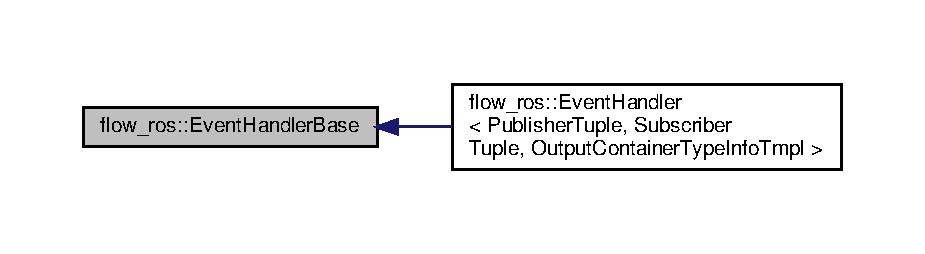
\includegraphics[width=350pt]{classflow__ros_1_1_event_handler_base__inherit__graph}
\end{center}
\end{figure}
\subsection*{Public Member Functions}
\begin{DoxyCompactItemize}
\item 
virtual \hyperlink{structflow__ros_1_1_event_summary}{Event\+Summary} \hyperlink{classflow__ros_1_1_event_handler_base_a5a4d9baa42d26f4d639b69ebbcc2aa0a}{update} (std\+::chrono\+::steady\+\_\+clock\+::time\+\_\+point timeout=std\+::chrono\+::steady\+\_\+clock\+::time\+\_\+point\+::max())=0
\begin{DoxyCompactList}\small\item\em Updates event handler. \end{DoxyCompactList}\item 
virtual \hyperlink{structflow__ros_1_1_event_summary}{Event\+Summary} \hyperlink{classflow__ros_1_1_event_handler_base_a85873d1e3eaa3c152295c5c49d5948f6}{dry\+\_\+update} ()=0
\begin{DoxyCompactList}\small\item\em Checks what synchronization result would be with current data. \end{DoxyCompactList}\item 
virtual void \hyperlink{classflow__ros_1_1_event_handler_base_a73c65bda396f3d8606e64487a7b30a76}{remove} (const ros\+::\+Time \&t\+\_\+remove)=0
\begin{DoxyCompactList}\small\item\em Removes all events before specified time. \end{DoxyCompactList}\item 
virtual void \hyperlink{classflow__ros_1_1_event_handler_base_a5611152cffdc62a4215726d19ce58ab5}{abort} (const ros\+::\+Time \&t\+\_\+abort)=0
\begin{DoxyCompactList}\small\item\em Aborts all event at or before specified time. \end{DoxyCompactList}\item 
\mbox{\Hypertarget{classflow__ros_1_1_event_handler_base_acd6151fd8c25f23c84fc4c815302f584}\label{classflow__ros_1_1_event_handler_base_acd6151fd8c25f23c84fc4c815302f584}} 
virtual void \hyperlink{classflow__ros_1_1_event_handler_base_acd6151fd8c25f23c84fc4c815302f584}{reset} ()=0
\begin{DoxyCompactList}\small\item\em Resets event handler and all managed channels. \end{DoxyCompactList}\item 
virtual std\+::vector$<$ std\+::shared\+\_\+ptr$<$ const \hyperlink{classflow__ros_1_1_publisher_base}{Publisher\+Base} $>$ $>$ \hyperlink{classflow__ros_1_1_event_handler_base_a1e476ba767ddceda60aadc5655ef33ed}{get\+Publishers} () const =0
\begin{DoxyCompactList}\small\item\em Returns vector of publisher resources associated with \hyperlink{classflow__ros_1_1_event_handler}{Event\+Handler}. \end{DoxyCompactList}\item 
virtual std\+::vector$<$ std\+::shared\+\_\+ptr$<$ const \hyperlink{classflow__ros_1_1_subscriber_base}{Subscriber\+Base} $>$ $>$ \hyperlink{classflow__ros_1_1_event_handler_base_a5c6b2e230dcb308eff3f0aea18c47be3}{get\+Subscribers} () const =0
\begin{DoxyCompactList}\small\item\em Returns vector of subscriber resources associated with \hyperlink{classflow__ros_1_1_event_handler}{Event\+Handler}. \end{DoxyCompactList}\end{DoxyCompactItemize}


\subsection{Detailed Description}
Event handler base type. 

\subsection{Member Function Documentation}
\mbox{\Hypertarget{classflow__ros_1_1_event_handler_base_a5611152cffdc62a4215726d19ce58ab5}\label{classflow__ros_1_1_event_handler_base_a5611152cffdc62a4215726d19ce58ab5}} 
\index{flow\+\_\+ros\+::\+Event\+Handler\+Base@{flow\+\_\+ros\+::\+Event\+Handler\+Base}!abort@{abort}}
\index{abort@{abort}!flow\+\_\+ros\+::\+Event\+Handler\+Base@{flow\+\_\+ros\+::\+Event\+Handler\+Base}}
\subsubsection{\texorpdfstring{abort()}{abort()}}
{\footnotesize\ttfamily virtual void flow\+\_\+ros\+::\+Event\+Handler\+Base\+::abort (\begin{DoxyParamCaption}\item[{const ros\+::\+Time \&}]{t\+\_\+abort }\end{DoxyParamCaption})\hspace{0.3cm}{\ttfamily [pure virtual]}}



Aborts all event at or before specified time. 


\begin{DoxyParams}{Parameters}
{\em t\+\_\+abort} & time before which events should be aborted \\
\hline
\end{DoxyParams}


Implemented in \hyperlink{classflow__ros_1_1_event_handler_a95200a36fc64725ac280c04c2697f709}{flow\+\_\+ros\+::\+Event\+Handler$<$ Publisher\+Tuple, Subscriber\+Tuple, Output\+Container\+Type\+Info\+Tmpl $>$}.

\mbox{\Hypertarget{classflow__ros_1_1_event_handler_base_a85873d1e3eaa3c152295c5c49d5948f6}\label{classflow__ros_1_1_event_handler_base_a85873d1e3eaa3c152295c5c49d5948f6}} 
\index{flow\+\_\+ros\+::\+Event\+Handler\+Base@{flow\+\_\+ros\+::\+Event\+Handler\+Base}!dry\+\_\+update@{dry\+\_\+update}}
\index{dry\+\_\+update@{dry\+\_\+update}!flow\+\_\+ros\+::\+Event\+Handler\+Base@{flow\+\_\+ros\+::\+Event\+Handler\+Base}}
\subsubsection{\texorpdfstring{dry\+\_\+update()}{dry\_update()}}
{\footnotesize\ttfamily virtual \hyperlink{structflow__ros_1_1_event_summary}{Event\+Summary} flow\+\_\+ros\+::\+Event\+Handler\+Base\+::dry\+\_\+update (\begin{DoxyParamCaption}{ }\end{DoxyParamCaption})\hspace{0.3cm}{\ttfamily [pure virtual]}}



Checks what synchronization result would be with current data. 

Performs no data waits, and skips actual capture

\begin{DoxyReturn}{Returns}
summary of potential event states on next {\ttfamily update} 
\end{DoxyReturn}


Implemented in \hyperlink{classflow__ros_1_1_event_handler_abc2f1821d85ab05d86270cbf20da6cd9}{flow\+\_\+ros\+::\+Event\+Handler$<$ Publisher\+Tuple, Subscriber\+Tuple, Output\+Container\+Type\+Info\+Tmpl $>$}.

\mbox{\Hypertarget{classflow__ros_1_1_event_handler_base_a1e476ba767ddceda60aadc5655ef33ed}\label{classflow__ros_1_1_event_handler_base_a1e476ba767ddceda60aadc5655ef33ed}} 
\index{flow\+\_\+ros\+::\+Event\+Handler\+Base@{flow\+\_\+ros\+::\+Event\+Handler\+Base}!get\+Publishers@{get\+Publishers}}
\index{get\+Publishers@{get\+Publishers}!flow\+\_\+ros\+::\+Event\+Handler\+Base@{flow\+\_\+ros\+::\+Event\+Handler\+Base}}
\subsubsection{\texorpdfstring{get\+Publishers()}{getPublishers()}}
{\footnotesize\ttfamily virtual std\+::vector$<$std\+::shared\+\_\+ptr$<$const \hyperlink{classflow__ros_1_1_publisher_base}{Publisher\+Base}$>$ $>$ flow\+\_\+ros\+::\+Event\+Handler\+Base\+::get\+Publishers (\begin{DoxyParamCaption}{ }\end{DoxyParamCaption}) const\hspace{0.3cm}{\ttfamily [pure virtual]}}



Returns vector of publisher resources associated with \hyperlink{classflow__ros_1_1_event_handler}{Event\+Handler}. 

\begin{DoxyNote}{Note}
Resource pointers in return value provide partial access to meta information about \hyperlink{classflow__ros_1_1_publisher}{Publisher} objects, but do not allow for data mutation 
\end{DoxyNote}


Implemented in \hyperlink{classflow__ros_1_1_event_handler_ae786846cf4cf48b9b952265862e73ef1}{flow\+\_\+ros\+::\+Event\+Handler$<$ Publisher\+Tuple, Subscriber\+Tuple, Output\+Container\+Type\+Info\+Tmpl $>$}.

\mbox{\Hypertarget{classflow__ros_1_1_event_handler_base_a5c6b2e230dcb308eff3f0aea18c47be3}\label{classflow__ros_1_1_event_handler_base_a5c6b2e230dcb308eff3f0aea18c47be3}} 
\index{flow\+\_\+ros\+::\+Event\+Handler\+Base@{flow\+\_\+ros\+::\+Event\+Handler\+Base}!get\+Subscribers@{get\+Subscribers}}
\index{get\+Subscribers@{get\+Subscribers}!flow\+\_\+ros\+::\+Event\+Handler\+Base@{flow\+\_\+ros\+::\+Event\+Handler\+Base}}
\subsubsection{\texorpdfstring{get\+Subscribers()}{getSubscribers()}}
{\footnotesize\ttfamily virtual std\+::vector$<$std\+::shared\+\_\+ptr$<$const \hyperlink{classflow__ros_1_1_subscriber_base}{Subscriber\+Base}$>$ $>$ flow\+\_\+ros\+::\+Event\+Handler\+Base\+::get\+Subscribers (\begin{DoxyParamCaption}{ }\end{DoxyParamCaption}) const\hspace{0.3cm}{\ttfamily [pure virtual]}}



Returns vector of subscriber resources associated with \hyperlink{classflow__ros_1_1_event_handler}{Event\+Handler}. 

\begin{DoxyNote}{Note}
Resource pointers in return value provide partial access to meta information about \hyperlink{classflow__ros_1_1_publisher}{Publisher} objects, but do not allow for data mutation 
\end{DoxyNote}


Implemented in \hyperlink{classflow__ros_1_1_event_handler_ac91cf67be38d79d3d86a9aa6318eca53}{flow\+\_\+ros\+::\+Event\+Handler$<$ Publisher\+Tuple, Subscriber\+Tuple, Output\+Container\+Type\+Info\+Tmpl $>$}.

\mbox{\Hypertarget{classflow__ros_1_1_event_handler_base_a73c65bda396f3d8606e64487a7b30a76}\label{classflow__ros_1_1_event_handler_base_a73c65bda396f3d8606e64487a7b30a76}} 
\index{flow\+\_\+ros\+::\+Event\+Handler\+Base@{flow\+\_\+ros\+::\+Event\+Handler\+Base}!remove@{remove}}
\index{remove@{remove}!flow\+\_\+ros\+::\+Event\+Handler\+Base@{flow\+\_\+ros\+::\+Event\+Handler\+Base}}
\subsubsection{\texorpdfstring{remove()}{remove()}}
{\footnotesize\ttfamily virtual void flow\+\_\+ros\+::\+Event\+Handler\+Base\+::remove (\begin{DoxyParamCaption}\item[{const ros\+::\+Time \&}]{t\+\_\+remove }\end{DoxyParamCaption})\hspace{0.3cm}{\ttfamily [pure virtual]}}



Removes all events before specified time. 


\begin{DoxyParams}{Parameters}
{\em t\+\_\+remove} & time before which events should be removed \\
\hline
\end{DoxyParams}


Implemented in \hyperlink{classflow__ros_1_1_event_handler_aeaf45592fd8c7fe8c3a4b0da23496d69}{flow\+\_\+ros\+::\+Event\+Handler$<$ Publisher\+Tuple, Subscriber\+Tuple, Output\+Container\+Type\+Info\+Tmpl $>$}.

\mbox{\Hypertarget{classflow__ros_1_1_event_handler_base_a5a4d9baa42d26f4d639b69ebbcc2aa0a}\label{classflow__ros_1_1_event_handler_base_a5a4d9baa42d26f4d639b69ebbcc2aa0a}} 
\index{flow\+\_\+ros\+::\+Event\+Handler\+Base@{flow\+\_\+ros\+::\+Event\+Handler\+Base}!update@{update}}
\index{update@{update}!flow\+\_\+ros\+::\+Event\+Handler\+Base@{flow\+\_\+ros\+::\+Event\+Handler\+Base}}
\subsubsection{\texorpdfstring{update()}{update()}}
{\footnotesize\ttfamily virtual \hyperlink{structflow__ros_1_1_event_summary}{Event\+Summary} flow\+\_\+ros\+::\+Event\+Handler\+Base\+::update (\begin{DoxyParamCaption}\item[{std\+::chrono\+::steady\+\_\+clock\+::time\+\_\+point}]{timeout = {\ttfamily std\+:\+:chrono\+:\+:steady\+\_\+clock\+:\+:time\+\_\+point\+:\+:max()} }\end{DoxyParamCaption})\hspace{0.3cm}{\ttfamily [pure virtual]}}



Updates event handler. 

\begin{DoxyReturn}{Returns}
summary of event states 
\end{DoxyReturn}


Implemented in \hyperlink{classflow__ros_1_1_event_handler_a445ecc20268a455bf47df8598413ae67}{flow\+\_\+ros\+::\+Event\+Handler$<$ Publisher\+Tuple, Subscriber\+Tuple, Output\+Container\+Type\+Info\+Tmpl $>$}.



The documentation for this class was generated from the following file\+:\begin{DoxyCompactItemize}
\item 
flow\+\_\+ros/include/\hyperlink{event__handler_8h}{event\+\_\+handler.\+h}\end{DoxyCompactItemize}

\hypertarget{structflow__ros_1_1detail_1_1_event_handler_input_type}{}\section{flow\+\_\+ros\+:\+:detail\+:\+:Event\+Handler\+Input\+Type$<$ Output\+Container\+Type\+Info\+Tmpl, Subscriber\+Tuple\+Type $>$ Struct Template Reference}
\label{structflow__ros_1_1detail_1_1_event_handler_input_type}\index{flow\+\_\+ros\+::detail\+::\+Event\+Handler\+Input\+Type$<$ Output\+Container\+Type\+Info\+Tmpl, Subscriber\+Tuple\+Type $>$@{flow\+\_\+ros\+::detail\+::\+Event\+Handler\+Input\+Type$<$ Output\+Container\+Type\+Info\+Tmpl, Subscriber\+Tuple\+Type $>$}}


Generates event callback input type for an \hyperlink{classflow__ros_1_1_event_handler}{Event\+Handler}.  




{\ttfamily \#include $<$event\+\_\+handler.\+hpp$>$}



\subsection{Detailed Description}
\subsubsection*{template$<$template$<$ typename $>$ class Output\+Container\+Type\+Info\+Tmpl, typename Subscriber\+Tuple\+Type$>$\newline
struct flow\+\_\+ros\+::detail\+::\+Event\+Handler\+Input\+Type$<$ Output\+Container\+Type\+Info\+Tmpl, Subscriber\+Tuple\+Type $>$}

Generates event callback input type for an \hyperlink{classflow__ros_1_1_event_handler}{Event\+Handler}. 

The documentation for this struct was generated from the following file\+:\begin{DoxyCompactItemize}
\item 
flow\+\_\+ros/include/impl/event\+\_\+handler.\+hpp\end{DoxyCompactItemize}

\hypertarget{structflow__ros_1_1detail_1_1_event_handler_input_type_3_01_output_container_type_info_tmpl_00_0ffddcead573ab44a62afad7bf9d6e18f}{}\section{flow\+\_\+ros\+:\+:detail\+:\+:Event\+Handler\+Input\+Type$<$ Output\+Container\+Type\+Info\+Tmpl, std\+:\+:tuple$<$ Subscriber\+Ts... $>$ $>$ Struct Template Reference}
\label{structflow__ros_1_1detail_1_1_event_handler_input_type_3_01_output_container_type_info_tmpl_00_0ffddcead573ab44a62afad7bf9d6e18f}\index{flow\+\_\+ros\+::detail\+::\+Event\+Handler\+Input\+Type$<$ Output\+Container\+Type\+Info\+Tmpl, std\+::tuple$<$ Subscriber\+Ts... $>$ $>$@{flow\+\_\+ros\+::detail\+::\+Event\+Handler\+Input\+Type$<$ Output\+Container\+Type\+Info\+Tmpl, std\+::tuple$<$ Subscriber\+Ts... $>$ $>$}}


Generates event callback input type for an \hyperlink{classflow__ros_1_1_event_handler}{Event\+Handler} with multiple outputs.  




{\ttfamily \#include $<$event\+\_\+handler.\+hpp$>$}

\subsection*{Public Types}
\begin{DoxyCompactItemize}
\item 
\mbox{\Hypertarget{structflow__ros_1_1detail_1_1_event_handler_input_type_3_01_output_container_type_info_tmpl_00_0ffddcead573ab44a62afad7bf9d6e18f_ada295a642648ff82f3544e8d00817b6a}\label{structflow__ros_1_1detail_1_1_event_handler_input_type_3_01_output_container_type_info_tmpl_00_0ffddcead573ab44a62afad7bf9d6e18f_ada295a642648ff82f3544e8d00817b6a}} 
using {\bfseries type} = std\+::tuple$<$ typename Output\+Container\+Type\+Info\+Tmpl$<$ typename \+::flow\+::\+Captor\+Traits$<$ typename \hyperlink{structflow__ros_1_1_subscriber_traits}{Subscriber\+Traits}$<$ Subscriber\+Ts $>$\+::Policy\+Type $>$\+::Dispatch\+Type $>$\+::Container... $>$
\end{DoxyCompactItemize}


\subsection{Detailed Description}
\subsubsection*{template$<$template$<$ typename $>$ class Output\+Container\+Type\+Info\+Tmpl, typename... Subscriber\+Ts$>$\newline
struct flow\+\_\+ros\+::detail\+::\+Event\+Handler\+Input\+Type$<$ Output\+Container\+Type\+Info\+Tmpl, std\+::tuple$<$ Subscriber\+Ts... $>$ $>$}

Generates event callback input type for an \hyperlink{classflow__ros_1_1_event_handler}{Event\+Handler} with multiple outputs. 

The documentation for this struct was generated from the following file\+:\begin{DoxyCompactItemize}
\item 
flow\+\_\+ros/include/impl/event\+\_\+handler.\+hpp\end{DoxyCompactItemize}

\hypertarget{structflow__ros_1_1detail_1_1_event_handler_output_type}{}\section{flow\+\_\+ros\+:\+:detail\+:\+:Event\+Handler\+Output\+Type$<$ Publisher\+TupleT $>$ Struct Template Reference}
\label{structflow__ros_1_1detail_1_1_event_handler_output_type}\index{flow\+\_\+ros\+::detail\+::\+Event\+Handler\+Output\+Type$<$ Publisher\+Tuple\+T $>$@{flow\+\_\+ros\+::detail\+::\+Event\+Handler\+Output\+Type$<$ Publisher\+Tuple\+T $>$}}


Generates event callback output type for an \hyperlink{classflow__ros_1_1_event_handler}{Event\+Handler} with a single output.  




{\ttfamily \#include $<$event\+\_\+handler.\+hpp$>$}

\subsection*{Public Types}
\begin{DoxyCompactItemize}
\item 
\mbox{\Hypertarget{structflow__ros_1_1detail_1_1_event_handler_output_type_a4f1b96df4f12596bd3ae2991a1335c26}\label{structflow__ros_1_1detail_1_1_event_handler_output_type_a4f1b96df4f12596bd3ae2991a1335c26}} 
using {\bfseries type} = typename \hyperlink{structflow__ros_1_1_publisher_traits}{Publisher\+Traits}$<$ Publisher\+TupleT $>$\+::Output\+Type
\end{DoxyCompactItemize}


\subsection{Detailed Description}
\subsubsection*{template$<$typename Publisher\+TupleT$>$\newline
struct flow\+\_\+ros\+::detail\+::\+Event\+Handler\+Output\+Type$<$ Publisher\+Tuple\+T $>$}

Generates event callback output type for an \hyperlink{classflow__ros_1_1_event_handler}{Event\+Handler} with a single output. 

The documentation for this struct was generated from the following file\+:\begin{DoxyCompactItemize}
\item 
flow\+\_\+ros/include/impl/event\+\_\+handler.\+hpp\end{DoxyCompactItemize}

\hypertarget{structflow__ros_1_1detail_1_1_event_handler_output_type_3_01std_1_1tuple_3_01_publisher_ts_8_8_8_01_4_01_4}{}\section{flow\+\_\+ros\+:\+:detail\+:\+:Event\+Handler\+Output\+Type$<$ std\+:\+:tuple$<$ Publisher\+Ts... $>$ $>$ Struct Template Reference}
\label{structflow__ros_1_1detail_1_1_event_handler_output_type_3_01std_1_1tuple_3_01_publisher_ts_8_8_8_01_4_01_4}\index{flow\+\_\+ros\+::detail\+::\+Event\+Handler\+Output\+Type$<$ std\+::tuple$<$ Publisher\+Ts... $>$ $>$@{flow\+\_\+ros\+::detail\+::\+Event\+Handler\+Output\+Type$<$ std\+::tuple$<$ Publisher\+Ts... $>$ $>$}}


Generates event callback output type for an \hyperlink{classflow__ros_1_1_event_handler}{Event\+Handler} with multiple outputs.  




{\ttfamily \#include $<$event\+\_\+handler.\+hpp$>$}

\subsection*{Public Types}
\begin{DoxyCompactItemize}
\item 
\mbox{\Hypertarget{structflow__ros_1_1detail_1_1_event_handler_output_type_3_01std_1_1tuple_3_01_publisher_ts_8_8_8_01_4_01_4_a898c9b0937975f04f3401de8f349a2f1}\label{structflow__ros_1_1detail_1_1_event_handler_output_type_3_01std_1_1tuple_3_01_publisher_ts_8_8_8_01_4_01_4_a898c9b0937975f04f3401de8f349a2f1}} 
using {\bfseries type} = std\+::tuple$<$ typename \hyperlink{structflow__ros_1_1_publisher_traits}{Publisher\+Traits}$<$ Publisher\+Ts $>$\+::Output\+Type... $>$
\end{DoxyCompactItemize}


\subsection{Detailed Description}
\subsubsection*{template$<$typename... Publisher\+Ts$>$\newline
struct flow\+\_\+ros\+::detail\+::\+Event\+Handler\+Output\+Type$<$ std\+::tuple$<$ Publisher\+Ts... $>$ $>$}

Generates event callback output type for an \hyperlink{classflow__ros_1_1_event_handler}{Event\+Handler} with multiple outputs. 

The documentation for this struct was generated from the following file\+:\begin{DoxyCompactItemize}
\item 
flow\+\_\+ros/include/impl/event\+\_\+handler.\+hpp\end{DoxyCompactItemize}

\hypertarget{structflow__ros_1_1detail_1_1_event_handler_output_type_3_01std_1_1tuple_3_4_01_4}{}\section{flow\+\_\+ros\+:\+:detail\+:\+:Event\+Handler\+Output\+Type$<$ std\+:\+:tuple$<$$>$ $>$ Struct Template Reference}
\label{structflow__ros_1_1detail_1_1_event_handler_output_type_3_01std_1_1tuple_3_4_01_4}\index{flow\+\_\+ros\+::detail\+::\+Event\+Handler\+Output\+Type$<$ std\+::tuple$<$$>$ $>$@{flow\+\_\+ros\+::detail\+::\+Event\+Handler\+Output\+Type$<$ std\+::tuple$<$$>$ $>$}}


Generates event callback output type for an \hyperlink{classflow__ros_1_1_event_handler}{Event\+Handler} with NO outputs.  




{\ttfamily \#include $<$event\+\_\+handler.\+hpp$>$}

\subsection*{Public Types}
\begin{DoxyCompactItemize}
\item 
\mbox{\Hypertarget{structflow__ros_1_1detail_1_1_event_handler_output_type_3_01std_1_1tuple_3_4_01_4_a73c49dba0af507dd3d1b00d0cc81c7fb}\label{structflow__ros_1_1detail_1_1_event_handler_output_type_3_01std_1_1tuple_3_4_01_4_a73c49dba0af507dd3d1b00d0cc81c7fb}} 
using {\bfseries type} = std\+::tuple$<$$>$
\end{DoxyCompactItemize}


\subsection{Detailed Description}
\subsubsection*{template$<$$>$\newline
struct flow\+\_\+ros\+::detail\+::\+Event\+Handler\+Output\+Type$<$ std\+::tuple$<$$>$ $>$}

Generates event callback output type for an \hyperlink{classflow__ros_1_1_event_handler}{Event\+Handler} with NO outputs. 

The documentation for this struct was generated from the following file\+:\begin{DoxyCompactItemize}
\item 
flow\+\_\+ros/include/impl/event\+\_\+handler.\+hpp\end{DoxyCompactItemize}

\hypertarget{classflow__ros_1_1detail_1_1_event_handler_publish_helper}{}\section{flow\+\_\+ros\+:\+:detail\+:\+:Event\+Handler\+Publish\+Helper Class Reference}
\label{classflow__ros_1_1detail_1_1_event_handler_publish_helper}\index{flow\+\_\+ros\+::detail\+::\+Event\+Handler\+Publish\+Helper@{flow\+\_\+ros\+::detail\+::\+Event\+Handler\+Publish\+Helper}}


Helper object used to publish 1 or N outputs from an \hyperlink{classflow__ros_1_1_event_handler}{Event\+Handler}.  




{\ttfamily \#include $<$event\+\_\+handler.\+hpp$>$}

\subsection*{Public Member Functions}
\begin{DoxyCompactItemize}
\item 
\mbox{\Hypertarget{classflow__ros_1_1detail_1_1_event_handler_publish_helper_a03b4f1bab44068d8de9e7350b0017432}\label{classflow__ros_1_1detail_1_1_event_handler_publish_helper_a03b4f1bab44068d8de9e7350b0017432}} 
{\bfseries Event\+Handler\+Publish\+Helper} (const ros\+::\+Time stamp)
\item 
\mbox{\Hypertarget{classflow__ros_1_1detail_1_1_event_handler_publish_helper_a8c5d9219369b2c85e9a3ad231ce57987}\label{classflow__ros_1_1detail_1_1_event_handler_publish_helper_a8c5d9219369b2c85e9a3ad231ce57987}} 
{\footnotesize template$<$typename PubT , typename OutputT $>$ }\\void \hyperlink{classflow__ros_1_1detail_1_1_event_handler_publish_helper_a8c5d9219369b2c85e9a3ad231ce57987}{operator()} (std\+::shared\+\_\+ptr$<$ PubT $>$ \&pub, OutputT \&\&output) const
\begin{DoxyCompactList}\small\item\em Publishes multiple messages through a publisher implementation. \end{DoxyCompactList}\end{DoxyCompactItemize}


\subsection{Detailed Description}
Helper object used to publish 1 or N outputs from an \hyperlink{classflow__ros_1_1_event_handler}{Event\+Handler}. 

The documentation for this class was generated from the following file\+:\begin{DoxyCompactItemize}
\item 
flow\+\_\+ros/include/impl/event\+\_\+handler.\+hpp\end{DoxyCompactItemize}

\hypertarget{structflow__ros_1_1_event_summary}{}\section{flow\+\_\+ros\+:\+:Event\+Summary Struct Reference}
\label{structflow__ros_1_1_event_summary}\index{flow\+\_\+ros\+::\+Event\+Summary@{flow\+\_\+ros\+::\+Event\+Summary}}


Summary of event information from results.  




{\ttfamily \#include $<$event\+\_\+handler.\+h$>$}

\subsection*{Public Types}
\begin{DoxyCompactItemize}
\item 
\mbox{\Hypertarget{structflow__ros_1_1_event_summary_a9b5a677b4629e3c40e36a49a3f2cea6b}\label{structflow__ros_1_1_event_summary_a9b5a677b4629e3c40e36a49a3f2cea6b}} 
enum \hyperlink{structflow__ros_1_1_event_summary_a9b5a677b4629e3c40e36a49a3f2cea6b}{State} \{ \newline
{\bfseries U\+N\+K\+N\+O\+WN}, 
{\bfseries E\+X\+E\+C\+U\+T\+ED}, 
{\bfseries E\+X\+E\+C\+U\+T\+I\+O\+N\+\_\+\+B\+Y\+P\+A\+S\+S\+ED}, 
{\bfseries S\+Y\+N\+C\+\_\+\+N\+E\+E\+D\+S\+\_\+\+R\+E\+T\+RY}, 
\newline
{\bfseries S\+Y\+N\+C\+\_\+\+A\+B\+O\+R\+T\+ED}, 
{\bfseries S\+Y\+N\+C\+\_\+\+T\+I\+M\+E\+D\+\_\+\+O\+UT}
 \}\begin{DoxyCompactList}\small\item\em Summary state codes. \end{DoxyCompactList}
\end{DoxyCompactItemize}
\subsection*{Public Member Functions}
\begin{DoxyCompactItemize}
\item 
\hyperlink{structflow__ros_1_1_event_summary_af5403b915dc7bb690c216e445c12d655}{Event\+Summary} (const flow\+::\+Result$<$ ros\+::\+Time $>$ \&\+\_\+result, const std\+::chrono\+::steady\+\_\+clock\+::time\+\_\+point \+\_\+execution\+\_\+timeout)
\begin{DoxyCompactList}\small\item\em Constructor for initialization from sync results. \end{DoxyCompactList}\end{DoxyCompactItemize}
\subsection*{Public Attributes}
\begin{DoxyCompactItemize}
\item 
\mbox{\Hypertarget{structflow__ros_1_1_event_summary_a194fe981559bf6e9bc814742a5b36b02}\label{structflow__ros_1_1_event_summary_a194fe981559bf6e9bc814742a5b36b02}} 
\hyperlink{structflow__ros_1_1_event_summary_a9b5a677b4629e3c40e36a49a3f2cea6b}{State} \hyperlink{structflow__ros_1_1_event_summary_a194fe981559bf6e9bc814742a5b36b02}{state}
\begin{DoxyCompactList}\small\item\em Event state. \end{DoxyCompactList}\item 
\mbox{\Hypertarget{structflow__ros_1_1_event_summary_a2c6cd6d0c869888e4783a365b5c20c4d}\label{structflow__ros_1_1_event_summary_a2c6cd6d0c869888e4783a365b5c20c4d}} 
flow\+::\+Capture\+Range$<$ ros\+::\+Time $>$ \hyperlink{structflow__ros_1_1_event_summary_a2c6cd6d0c869888e4783a365b5c20c4d}{range}
\begin{DoxyCompactList}\small\item\em Capture time range. \end{DoxyCompactList}\item 
\mbox{\Hypertarget{structflow__ros_1_1_event_summary_a18cd625e078cc5af161087134a28bd8f}\label{structflow__ros_1_1_event_summary_a18cd625e078cc5af161087134a28bd8f}} 
std\+::chrono\+::steady\+\_\+clock\+::time\+\_\+point \hyperlink{structflow__ros_1_1_event_summary_a18cd625e078cc5af161087134a28bd8f}{execution\+\_\+timeout}
\begin{DoxyCompactList}\small\item\em Execution timeout. \end{DoxyCompactList}\end{DoxyCompactItemize}


\subsection{Detailed Description}
Summary of event information from results. 

\subsection{Constructor \& Destructor Documentation}
\mbox{\Hypertarget{structflow__ros_1_1_event_summary_af5403b915dc7bb690c216e445c12d655}\label{structflow__ros_1_1_event_summary_af5403b915dc7bb690c216e445c12d655}} 
\index{flow\+\_\+ros\+::\+Event\+Summary@{flow\+\_\+ros\+::\+Event\+Summary}!Event\+Summary@{Event\+Summary}}
\index{Event\+Summary@{Event\+Summary}!flow\+\_\+ros\+::\+Event\+Summary@{flow\+\_\+ros\+::\+Event\+Summary}}
\subsubsection{\texorpdfstring{Event\+Summary()}{EventSummary()}}
{\footnotesize\ttfamily flow\+\_\+ros\+::\+Event\+Summary\+::\+Event\+Summary (\begin{DoxyParamCaption}\item[{const flow\+::\+Result$<$ ros\+::\+Time $>$ \&}]{\+\_\+result,  }\item[{const std\+::chrono\+::steady\+\_\+clock\+::time\+\_\+point}]{\+\_\+execution\+\_\+timeout }\end{DoxyParamCaption})\hspace{0.3cm}{\ttfamily [inline]}}



Constructor for initialization from sync results. 


\begin{DoxyParams}{Parameters}
{\em \+\_\+result} & synchronizer result information \\
\hline
{\em \+\_\+execution\+\_\+timeout} & system-\/time point for execution timeout \\
\hline
\end{DoxyParams}


The documentation for this struct was generated from the following file\+:\begin{DoxyCompactItemize}
\item 
flow\+\_\+ros/include/\hyperlink{event__handler_8h}{event\+\_\+handler.\+h}\end{DoxyCompactItemize}

\hypertarget{structflow_1_1is__driver_3_1_1flow__ros_1_1_subscriber_3_01_msg_t_00_01_policy_tmpl_00_01_lock_policy_t_01_4_01_4}{}\section{flow\+:\+:is\+\_\+driver$<$\+:\+:flow\+\_\+ros\+:\+:Subscriber$<$ MsgT, Policy\+Tmpl, Lock\+PolicyT $>$ $>$ Struct Template Reference}
\label{structflow_1_1is__driver_3_1_1flow__ros_1_1_subscriber_3_01_msg_t_00_01_policy_tmpl_00_01_lock_policy_t_01_4_01_4}\index{flow\+::is\+\_\+driver$<$\+::flow\+\_\+ros\+::\+Subscriber$<$ Msg\+T, Policy\+Tmpl, Lock\+Policy\+T $>$ $>$@{flow\+::is\+\_\+driver$<$\+::flow\+\_\+ros\+::\+Subscriber$<$ Msg\+T, Policy\+Tmpl, Lock\+Policy\+T $>$ $>$}}


Checks if subscriber capture policy is derived from a Driver base.  




{\ttfamily \#include $<$subscriber.\+h$>$}



Inheritance diagram for flow\+:\+:is\+\_\+driver$<$\+:\+:flow\+\_\+ros\+:\+:Subscriber$<$ MsgT, Policy\+Tmpl, Lock\+PolicyT $>$ $>$\+:\nopagebreak
\begin{figure}[H]
\begin{center}
\leavevmode
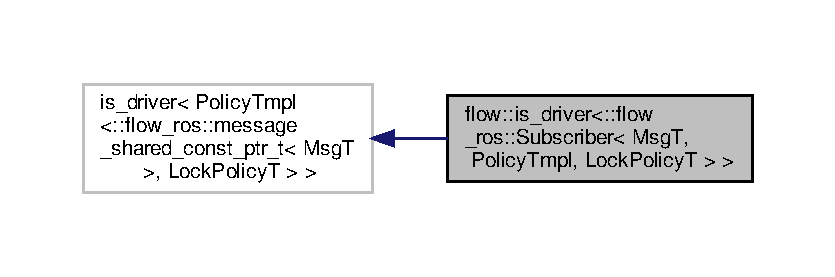
\includegraphics[width=350pt]{structflow_1_1is__driver_3_1_1flow__ros_1_1_subscriber_3_01_msg_t_00_01_policy_tmpl_00_01_lock_pad823e27bc9f39ecff1cc3ffbaaad8f4}
\end{center}
\end{figure}


Collaboration diagram for flow\+:\+:is\+\_\+driver$<$\+:\+:flow\+\_\+ros\+:\+:Subscriber$<$ MsgT, Policy\+Tmpl, Lock\+PolicyT $>$ $>$\+:\nopagebreak
\begin{figure}[H]
\begin{center}
\leavevmode
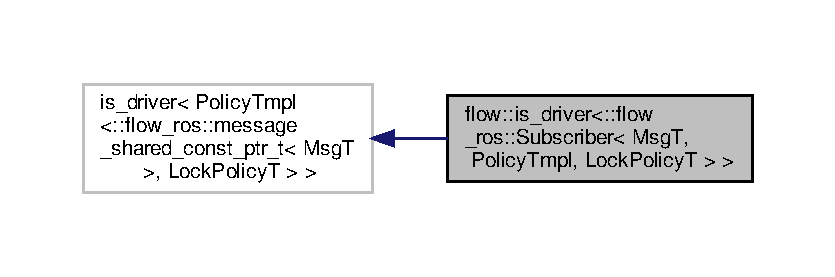
\includegraphics[width=350pt]{structflow_1_1is__driver_3_1_1flow__ros_1_1_subscriber_3_01_msg_t_00_01_policy_tmpl_00_01_lock_policy_t_01_4_01_4__coll__graph}
\end{center}
\end{figure}


\subsection{Detailed Description}
\subsubsection*{template$<$typename MsgT, template$<$ typename... $>$ class Policy\+Tmpl, typename Lock\+PolicyT$>$\newline
struct flow\+::is\+\_\+driver$<$\+::flow\+\_\+ros\+::\+Subscriber$<$ Msg\+T, Policy\+Tmpl, Lock\+Policy\+T $>$ $>$}

Checks if subscriber capture policy is derived from a Driver base. 

The documentation for this struct was generated from the following file\+:\begin{DoxyCompactItemize}
\item 
flow\+\_\+ros/include/\hyperlink{subscriber_8h}{subscriber.\+h}\end{DoxyCompactItemize}

\hypertarget{structflow_1_1is__follower_3_1_1flow__ros_1_1_subscriber_3_01_msg_t_00_01_policy_tmpl_00_01_lock_policy_t_01_4_01_4}{}\section{flow\+:\+:is\+\_\+follower$<$\+:\+:flow\+\_\+ros\+:\+:Subscriber$<$ MsgT, Policy\+Tmpl, Lock\+PolicyT $>$ $>$ Struct Template Reference}
\label{structflow_1_1is__follower_3_1_1flow__ros_1_1_subscriber_3_01_msg_t_00_01_policy_tmpl_00_01_lock_policy_t_01_4_01_4}\index{flow\+::is\+\_\+follower$<$\+::flow\+\_\+ros\+::\+Subscriber$<$ Msg\+T, Policy\+Tmpl, Lock\+Policy\+T $>$ $>$@{flow\+::is\+\_\+follower$<$\+::flow\+\_\+ros\+::\+Subscriber$<$ Msg\+T, Policy\+Tmpl, Lock\+Policy\+T $>$ $>$}}


Checks if subscriber capture policy is derived from a Follower base.  




{\ttfamily \#include $<$subscriber.\+h$>$}



Inheritance diagram for flow\+:\+:is\+\_\+follower$<$\+:\+:flow\+\_\+ros\+:\+:Subscriber$<$ MsgT, Policy\+Tmpl, Lock\+PolicyT $>$ $>$\+:\nopagebreak
\begin{figure}[H]
\begin{center}
\leavevmode
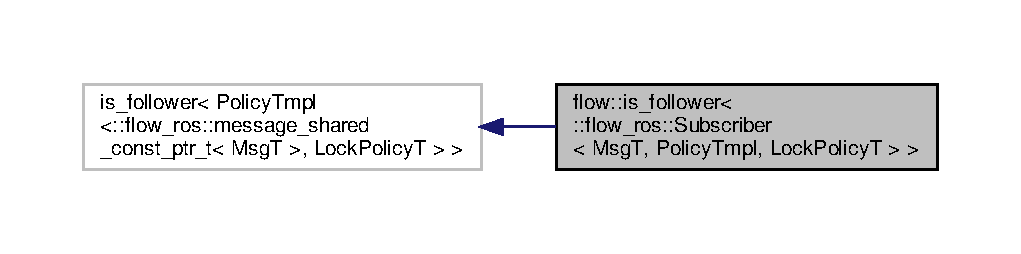
\includegraphics[width=350pt]{structflow_1_1is__follower_3_1_1flow__ros_1_1_subscriber_3_01_msg_t_00_01_policy_tmpl_00_01_lock05a79c2370d5be3b044e2172583e7cc1}
\end{center}
\end{figure}


Collaboration diagram for flow\+:\+:is\+\_\+follower$<$\+:\+:flow\+\_\+ros\+:\+:Subscriber$<$ MsgT, Policy\+Tmpl, Lock\+PolicyT $>$ $>$\+:\nopagebreak
\begin{figure}[H]
\begin{center}
\leavevmode
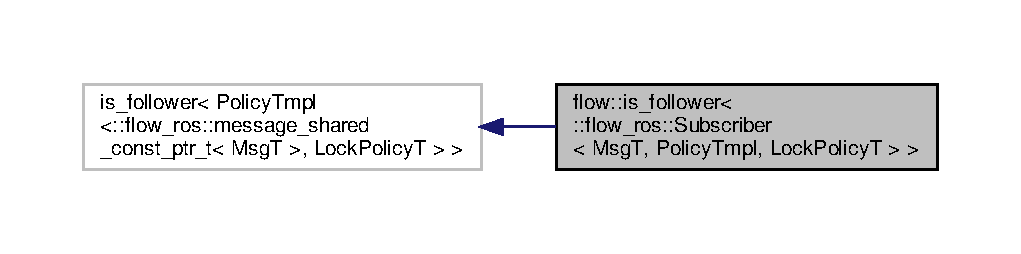
\includegraphics[width=350pt]{structflow_1_1is__follower_3_1_1flow__ros_1_1_subscriber_3_01_msg_t_00_01_policy_tmpl_00_01_lock46fa4a97b2692d84fdf345a45fec317b}
\end{center}
\end{figure}


\subsection{Detailed Description}
\subsubsection*{template$<$typename MsgT, template$<$ typename... $>$ class Policy\+Tmpl, typename Lock\+PolicyT$>$\newline
struct flow\+::is\+\_\+follower$<$\+::flow\+\_\+ros\+::\+Subscriber$<$ Msg\+T, Policy\+Tmpl, Lock\+Policy\+T $>$ $>$}

Checks if subscriber capture policy is derived from a Follower base. 

The documentation for this struct was generated from the following file\+:\begin{DoxyCompactItemize}
\item 
flow\+\_\+ros/include/\hyperlink{subscriber_8h}{subscriber.\+h}\end{DoxyCompactItemize}

\hypertarget{classflow__ros_1_1routing_1_1_local_publication}{}\section{flow\+\_\+ros\+:\+:routing\+:\+:Local\+Publication$<$ MsgT $>$ Class Template Reference}
\label{classflow__ros_1_1routing_1_1_local_publication}\index{flow\+\_\+ros\+::routing\+::\+Local\+Publication$<$ Msg\+T $>$@{flow\+\_\+ros\+::routing\+::\+Local\+Publication$<$ Msg\+T $>$}}


A Subscription object used for passing messages locally.  




{\ttfamily \#include $<$local\+\_\+publication.\+h$>$}



Inheritance diagram for flow\+\_\+ros\+:\+:routing\+:\+:Local\+Publication$<$ MsgT $>$\+:\nopagebreak
\begin{figure}[H]
\begin{center}
\leavevmode
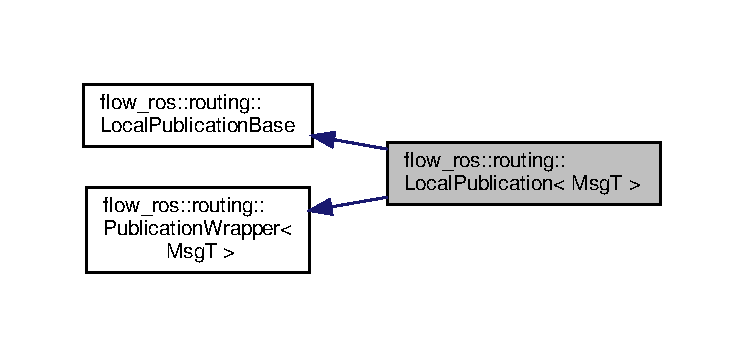
\includegraphics[width=350pt]{classflow__ros_1_1routing_1_1_local_publication__inherit__graph}
\end{center}
\end{figure}


Collaboration diagram for flow\+\_\+ros\+:\+:routing\+:\+:Local\+Publication$<$ MsgT $>$\+:\nopagebreak
\begin{figure}[H]
\begin{center}
\leavevmode
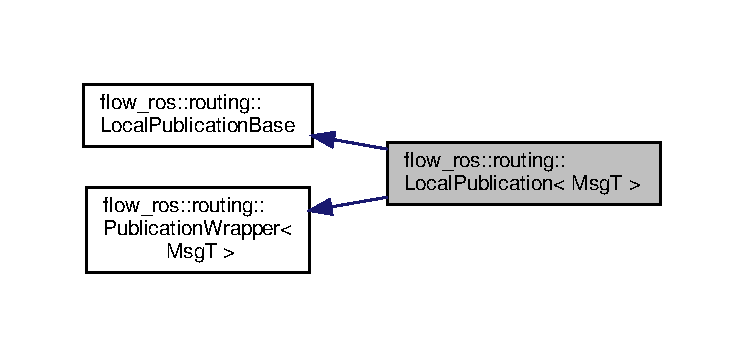
\includegraphics[width=350pt]{classflow__ros_1_1routing_1_1_local_publication__coll__graph}
\end{center}
\end{figure}
\subsection*{Public Member Functions}
\begin{DoxyCompactItemize}
\item 
\hyperlink{classflow__ros_1_1routing_1_1_local_publication_a1430b9009fbb39639d69faa0545b8ec8}{Local\+Publication} (std\+::string topic, std\+::shared\+\_\+ptr$<$ \hyperlink{classflow__ros_1_1routing_1_1_local_subscription_group}{Local\+Subscription\+Group} $>$ subscribers)
\begin{DoxyCompactList}\small\item\em Required setup constructor. \end{DoxyCompactList}\item 
void \hyperlink{classflow__ros_1_1routing_1_1_local_publication_ab2d53a2bd93e83ee11095f35d5820226}{publish} (const \hyperlink{namespaceflow__ros_a21a684f38ee2083b3858613317c46d82}{message\+\_\+shared\+\_\+ptr\+\_\+t}$<$ MsgT $>$ \&message) const
\begin{DoxyCompactList}\small\item\em Call all held subscriber callbacks on message being published. \end{DoxyCompactList}\item 
std\+::string \hyperlink{classflow__ros_1_1routing_1_1_local_publication_ab4d9ccc2b388dfe3db3ca1f4c1b0651d}{get\+Topic} () const override
\begin{DoxyCompactList}\small\item\em Returns topic associated with publication. \end{DoxyCompactList}\item 
std\+::uint32\+\_\+t \hyperlink{classflow__ros_1_1routing_1_1_local_publication_a3c79d6a426202a0ba0fad4f3de9e07b4}{get\+Num\+Subscribers} () const override
\begin{DoxyCompactList}\small\item\em Returns number of subscriptions connected to this publication. \end{DoxyCompactList}\item 
bool \hyperlink{classflow__ros_1_1routing_1_1_local_publication_ad1b48ed20ccdab599389f3132f545dd8}{is\+Latched} () const override
\begin{DoxyCompactList}\small\item\em Returns flag indicating whether or not publisher is latched. \end{DoxyCompactList}\item 
\hyperlink{transport__info_8h_ae57afcf849a5bdb82b958347c6ccc57b}{Transport\+Method} \hyperlink{classflow__ros_1_1routing_1_1_local_publication_a386554f0af2d80bdf566c496ea01b4b8}{get\+Transport\+Method} () const override
\item 
bool \hyperlink{classflow__ros_1_1routing_1_1_local_publication_a982359da6513c94f5befd4e990796c28}{is\+Valid} () const override
\end{DoxyCompactItemize}
\subsection*{Additional Inherited Members}


\subsection{Detailed Description}
\subsubsection*{template$<$typename MsgT$>$\newline
class flow\+\_\+ros\+::routing\+::\+Local\+Publication$<$ Msg\+T $>$}

A Subscription object used for passing messages locally. 


\begin{DoxyTemplParams}{Template Parameters}
{\em MsgT} & transported data type \\
\hline
\end{DoxyTemplParams}


\subsection{Constructor \& Destructor Documentation}
\mbox{\Hypertarget{classflow__ros_1_1routing_1_1_local_publication_a1430b9009fbb39639d69faa0545b8ec8}\label{classflow__ros_1_1routing_1_1_local_publication_a1430b9009fbb39639d69faa0545b8ec8}} 
\index{flow\+\_\+ros\+::routing\+::\+Local\+Publication@{flow\+\_\+ros\+::routing\+::\+Local\+Publication}!Local\+Publication@{Local\+Publication}}
\index{Local\+Publication@{Local\+Publication}!flow\+\_\+ros\+::routing\+::\+Local\+Publication@{flow\+\_\+ros\+::routing\+::\+Local\+Publication}}
\subsubsection{\texorpdfstring{Local\+Publication()}{LocalPublication()}}
{\footnotesize\ttfamily template$<$typename MsgT $>$ \\
\hyperlink{classflow__ros_1_1routing_1_1_local_publication}{flow\+\_\+ros\+::routing\+::\+Local\+Publication}$<$ MsgT $>$\+::\hyperlink{classflow__ros_1_1routing_1_1_local_publication}{Local\+Publication} (\begin{DoxyParamCaption}\item[{std\+::string}]{topic,  }\item[{std\+::shared\+\_\+ptr$<$ \hyperlink{classflow__ros_1_1routing_1_1_local_subscription_group}{Local\+Subscription\+Group} $>$}]{subscribers }\end{DoxyParamCaption})\hspace{0.3cm}{\ttfamily [inline]}}



Required setup constructor. 


\begin{DoxyParams}{Parameters}
{\em topic} & topic associated with published messages \\
\hline
{\em subscribers} & group of \hyperlink{classflow__ros_1_1routing_1_1_local_subscription}{Local\+Subscription} object which will be passed published messages \\
\hline
\end{DoxyParams}


\subsection{Member Function Documentation}
\mbox{\Hypertarget{classflow__ros_1_1routing_1_1_local_publication_a3c79d6a426202a0ba0fad4f3de9e07b4}\label{classflow__ros_1_1routing_1_1_local_publication_a3c79d6a426202a0ba0fad4f3de9e07b4}} 
\index{flow\+\_\+ros\+::routing\+::\+Local\+Publication@{flow\+\_\+ros\+::routing\+::\+Local\+Publication}!get\+Num\+Subscribers@{get\+Num\+Subscribers}}
\index{get\+Num\+Subscribers@{get\+Num\+Subscribers}!flow\+\_\+ros\+::routing\+::\+Local\+Publication@{flow\+\_\+ros\+::routing\+::\+Local\+Publication}}
\subsubsection{\texorpdfstring{get\+Num\+Subscribers()}{getNumSubscribers()}}
{\footnotesize\ttfamily template$<$typename MsgT $>$ \\
std\+::uint32\+\_\+t \hyperlink{classflow__ros_1_1routing_1_1_local_publication}{flow\+\_\+ros\+::routing\+::\+Local\+Publication}$<$ MsgT $>$\+::get\+Num\+Subscribers (\begin{DoxyParamCaption}{ }\end{DoxyParamCaption}) const\hspace{0.3cm}{\ttfamily [inline]}, {\ttfamily [override]}, {\ttfamily [virtual]}}



Returns number of subscriptions connected to this publication. 



Implements \hyperlink{classflow__ros_1_1routing_1_1_publication_wrapper_a3e2fb2a4cafe729a643af5ed5033dc50}{flow\+\_\+ros\+::routing\+::\+Publication\+Wrapper$<$ Msg\+T $>$}.

\mbox{\Hypertarget{classflow__ros_1_1routing_1_1_local_publication_ab4d9ccc2b388dfe3db3ca1f4c1b0651d}\label{classflow__ros_1_1routing_1_1_local_publication_ab4d9ccc2b388dfe3db3ca1f4c1b0651d}} 
\index{flow\+\_\+ros\+::routing\+::\+Local\+Publication@{flow\+\_\+ros\+::routing\+::\+Local\+Publication}!get\+Topic@{get\+Topic}}
\index{get\+Topic@{get\+Topic}!flow\+\_\+ros\+::routing\+::\+Local\+Publication@{flow\+\_\+ros\+::routing\+::\+Local\+Publication}}
\subsubsection{\texorpdfstring{get\+Topic()}{getTopic()}}
{\footnotesize\ttfamily template$<$typename MsgT $>$ \\
std\+::string \hyperlink{classflow__ros_1_1routing_1_1_local_publication}{flow\+\_\+ros\+::routing\+::\+Local\+Publication}$<$ MsgT $>$\+::get\+Topic (\begin{DoxyParamCaption}{ }\end{DoxyParamCaption}) const\hspace{0.3cm}{\ttfamily [inline]}, {\ttfamily [override]}, {\ttfamily [virtual]}}



Returns topic associated with publication. 



Implements \hyperlink{classflow__ros_1_1routing_1_1_publication_wrapper_a1aa441bb1846211cb803362233d4ee0b}{flow\+\_\+ros\+::routing\+::\+Publication\+Wrapper$<$ Msg\+T $>$}.

\mbox{\Hypertarget{classflow__ros_1_1routing_1_1_local_publication_a386554f0af2d80bdf566c496ea01b4b8}\label{classflow__ros_1_1routing_1_1_local_publication_a386554f0af2d80bdf566c496ea01b4b8}} 
\index{flow\+\_\+ros\+::routing\+::\+Local\+Publication@{flow\+\_\+ros\+::routing\+::\+Local\+Publication}!get\+Transport\+Method@{get\+Transport\+Method}}
\index{get\+Transport\+Method@{get\+Transport\+Method}!flow\+\_\+ros\+::routing\+::\+Local\+Publication@{flow\+\_\+ros\+::routing\+::\+Local\+Publication}}
\subsubsection{\texorpdfstring{get\+Transport\+Method()}{getTransportMethod()}}
{\footnotesize\ttfamily template$<$typename MsgT $>$ \\
\hyperlink{transport__info_8h_ae57afcf849a5bdb82b958347c6ccc57b}{Transport\+Method} \hyperlink{classflow__ros_1_1routing_1_1_local_publication}{flow\+\_\+ros\+::routing\+::\+Local\+Publication}$<$ MsgT $>$\+::get\+Transport\+Method (\begin{DoxyParamCaption}{ }\end{DoxyParamCaption}) const\hspace{0.3cm}{\ttfamily [inline]}, {\ttfamily [override]}, {\ttfamily [virtual]}}







Implements \hyperlink{classflow__ros_1_1routing_1_1_publication_wrapper_a0398202c79a6bdb1ff57acc8c730bc65}{flow\+\_\+ros\+::routing\+::\+Publication\+Wrapper$<$ Msg\+T $>$}.

\mbox{\Hypertarget{classflow__ros_1_1routing_1_1_local_publication_ad1b48ed20ccdab599389f3132f545dd8}\label{classflow__ros_1_1routing_1_1_local_publication_ad1b48ed20ccdab599389f3132f545dd8}} 
\index{flow\+\_\+ros\+::routing\+::\+Local\+Publication@{flow\+\_\+ros\+::routing\+::\+Local\+Publication}!is\+Latched@{is\+Latched}}
\index{is\+Latched@{is\+Latched}!flow\+\_\+ros\+::routing\+::\+Local\+Publication@{flow\+\_\+ros\+::routing\+::\+Local\+Publication}}
\subsubsection{\texorpdfstring{is\+Latched()}{isLatched()}}
{\footnotesize\ttfamily template$<$typename MsgT $>$ \\
bool \hyperlink{classflow__ros_1_1routing_1_1_local_publication}{flow\+\_\+ros\+::routing\+::\+Local\+Publication}$<$ MsgT $>$\+::is\+Latched (\begin{DoxyParamCaption}{ }\end{DoxyParamCaption}) const\hspace{0.3cm}{\ttfamily [inline]}, {\ttfamily [override]}, {\ttfamily [virtual]}}



Returns flag indicating whether or not publisher is latched. 

\begin{DoxyNote}{Note}
Dummy implementation; local publications cannot be latched 
\end{DoxyNote}


Implements \hyperlink{classflow__ros_1_1routing_1_1_publication_wrapper_a86fdc857e02347e862dbbb113e5a6cb6}{flow\+\_\+ros\+::routing\+::\+Publication\+Wrapper$<$ Msg\+T $>$}.

\mbox{\Hypertarget{classflow__ros_1_1routing_1_1_local_publication_a982359da6513c94f5befd4e990796c28}\label{classflow__ros_1_1routing_1_1_local_publication_a982359da6513c94f5befd4e990796c28}} 
\index{flow\+\_\+ros\+::routing\+::\+Local\+Publication@{flow\+\_\+ros\+::routing\+::\+Local\+Publication}!is\+Valid@{is\+Valid}}
\index{is\+Valid@{is\+Valid}!flow\+\_\+ros\+::routing\+::\+Local\+Publication@{flow\+\_\+ros\+::routing\+::\+Local\+Publication}}
\subsubsection{\texorpdfstring{is\+Valid()}{isValid()}}
{\footnotesize\ttfamily template$<$typename MsgT $>$ \\
bool \hyperlink{classflow__ros_1_1routing_1_1_local_publication}{flow\+\_\+ros\+::routing\+::\+Local\+Publication}$<$ MsgT $>$\+::is\+Valid (\begin{DoxyParamCaption}{ }\end{DoxyParamCaption}) const\hspace{0.3cm}{\ttfamily [inline]}, {\ttfamily [override]}, {\ttfamily [virtual]}}







Implements \hyperlink{classflow__ros_1_1routing_1_1_publication_wrapper_afc33bf27092f8e8188e3f7955a6b7c97}{flow\+\_\+ros\+::routing\+::\+Publication\+Wrapper$<$ Msg\+T $>$}.

\mbox{\Hypertarget{classflow__ros_1_1routing_1_1_local_publication_ab2d53a2bd93e83ee11095f35d5820226}\label{classflow__ros_1_1routing_1_1_local_publication_ab2d53a2bd93e83ee11095f35d5820226}} 
\index{flow\+\_\+ros\+::routing\+::\+Local\+Publication@{flow\+\_\+ros\+::routing\+::\+Local\+Publication}!publish@{publish}}
\index{publish@{publish}!flow\+\_\+ros\+::routing\+::\+Local\+Publication@{flow\+\_\+ros\+::routing\+::\+Local\+Publication}}
\subsubsection{\texorpdfstring{publish()}{publish()}}
{\footnotesize\ttfamily template$<$typename MsgT $>$ \\
void \hyperlink{classflow__ros_1_1routing_1_1_local_publication}{flow\+\_\+ros\+::routing\+::\+Local\+Publication}$<$ MsgT $>$\+::publish (\begin{DoxyParamCaption}\item[{const \hyperlink{namespaceflow__ros_a21a684f38ee2083b3858613317c46d82}{message\+\_\+shared\+\_\+ptr\+\_\+t}$<$ MsgT $>$ \&}]{message }\end{DoxyParamCaption}) const\hspace{0.3cm}{\ttfamily [inline]}, {\ttfamily [virtual]}}



Call all held subscriber callbacks on message being published. 


\begin{DoxyParams}{Parameters}
{\em message} & message data to publish \\
\hline
\end{DoxyParams}


Implements \hyperlink{classflow__ros_1_1routing_1_1_publication_wrapper_a43b9989390bf9f001fe9670a0c1d5897}{flow\+\_\+ros\+::routing\+::\+Publication\+Wrapper$<$ Msg\+T $>$}.



The documentation for this class was generated from the following file\+:\begin{DoxyCompactItemize}
\item 
flow\+\_\+ros/include/routing/local\+\_\+publication.\+h\end{DoxyCompactItemize}

\hypertarget{classflow__ros_1_1routing_1_1_local_publication_base}{}\section{flow\+\_\+ros\+:\+:routing\+:\+:Local\+Publication\+Base Class Reference}
\label{classflow__ros_1_1routing_1_1_local_publication_base}\index{flow\+\_\+ros\+::routing\+::\+Local\+Publication\+Base@{flow\+\_\+ros\+::routing\+::\+Local\+Publication\+Base}}


\hyperlink{classflow__ros_1_1routing_1_1_local_publication}{Local\+Publication} base which provides basic info and erases Msg\+T-\/dependent methods.  




{\ttfamily \#include $<$local\+\_\+publication.\+h$>$}



Inheritance diagram for flow\+\_\+ros\+:\+:routing\+:\+:Local\+Publication\+Base\+:\nopagebreak
\begin{figure}[H]
\begin{center}
\leavevmode
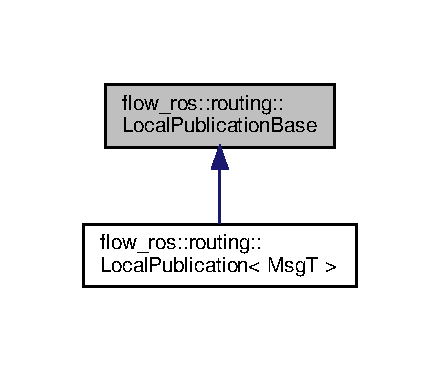
\includegraphics[width=211pt]{classflow__ros_1_1routing_1_1_local_publication_base__inherit__graph}
\end{center}
\end{figure}
\subsection*{Public Member Functions}
\begin{DoxyCompactItemize}
\item 
\hyperlink{classflow__ros_1_1routing_1_1_local_publication_base_af9fda03de061e405e283029280db322f}{Local\+Publication\+Base} (std\+::string topic)
\begin{DoxyCompactList}\small\item\em Topic setup constructor. \end{DoxyCompactList}\item 
const std\+::string \& \hyperlink{classflow__ros_1_1routing_1_1_local_publication_base_a3c5ed7bb057a44e05c7248cf908326ba}{get\+Topic} () const
\begin{DoxyCompactList}\small\item\em Returns topic associated with publication. \end{DoxyCompactList}\end{DoxyCompactItemize}


\subsection{Detailed Description}
\hyperlink{classflow__ros_1_1routing_1_1_local_publication}{Local\+Publication} base which provides basic info and erases Msg\+T-\/dependent methods. 

\subsection{Constructor \& Destructor Documentation}
\mbox{\Hypertarget{classflow__ros_1_1routing_1_1_local_publication_base_af9fda03de061e405e283029280db322f}\label{classflow__ros_1_1routing_1_1_local_publication_base_af9fda03de061e405e283029280db322f}} 
\index{flow\+\_\+ros\+::routing\+::\+Local\+Publication\+Base@{flow\+\_\+ros\+::routing\+::\+Local\+Publication\+Base}!Local\+Publication\+Base@{Local\+Publication\+Base}}
\index{Local\+Publication\+Base@{Local\+Publication\+Base}!flow\+\_\+ros\+::routing\+::\+Local\+Publication\+Base@{flow\+\_\+ros\+::routing\+::\+Local\+Publication\+Base}}
\subsubsection{\texorpdfstring{Local\+Publication\+Base()}{LocalPublicationBase()}}
{\footnotesize\ttfamily flow\+\_\+ros\+::routing\+::\+Local\+Publication\+Base\+::\+Local\+Publication\+Base (\begin{DoxyParamCaption}\item[{std\+::string}]{topic }\end{DoxyParamCaption})\hspace{0.3cm}{\ttfamily [inline]}, {\ttfamily [explicit]}}



Topic setup constructor. 


\begin{DoxyParams}{Parameters}
{\em topic} & topic name to associate with this object \\
\hline
\end{DoxyParams}


\subsection{Member Function Documentation}
\mbox{\Hypertarget{classflow__ros_1_1routing_1_1_local_publication_base_a3c5ed7bb057a44e05c7248cf908326ba}\label{classflow__ros_1_1routing_1_1_local_publication_base_a3c5ed7bb057a44e05c7248cf908326ba}} 
\index{flow\+\_\+ros\+::routing\+::\+Local\+Publication\+Base@{flow\+\_\+ros\+::routing\+::\+Local\+Publication\+Base}!get\+Topic@{get\+Topic}}
\index{get\+Topic@{get\+Topic}!flow\+\_\+ros\+::routing\+::\+Local\+Publication\+Base@{flow\+\_\+ros\+::routing\+::\+Local\+Publication\+Base}}
\subsubsection{\texorpdfstring{get\+Topic()}{getTopic()}}
{\footnotesize\ttfamily const std\+::string\& flow\+\_\+ros\+::routing\+::\+Local\+Publication\+Base\+::get\+Topic (\begin{DoxyParamCaption}{ }\end{DoxyParamCaption}) const\hspace{0.3cm}{\ttfamily [inline]}}



Returns topic associated with publication. 



The documentation for this class was generated from the following file\+:\begin{DoxyCompactItemize}
\item 
flow\+\_\+ros/include/routing/local\+\_\+publication.\+h\end{DoxyCompactItemize}

\hypertarget{classflow__ros_1_1routing_1_1_local_subscription}{}\section{flow\+\_\+ros\+:\+:routing\+:\+:Local\+Subscription$<$ MsgT $>$ Class Template Reference}
\label{classflow__ros_1_1routing_1_1_local_subscription}\index{flow\+\_\+ros\+::routing\+::\+Local\+Subscription$<$ Msg\+T $>$@{flow\+\_\+ros\+::routing\+::\+Local\+Subscription$<$ Msg\+T $>$}}


Inheritance diagram for flow\+\_\+ros\+:\+:routing\+:\+:Local\+Subscription$<$ MsgT $>$\+:\nopagebreak
\begin{figure}[H]
\begin{center}
\leavevmode
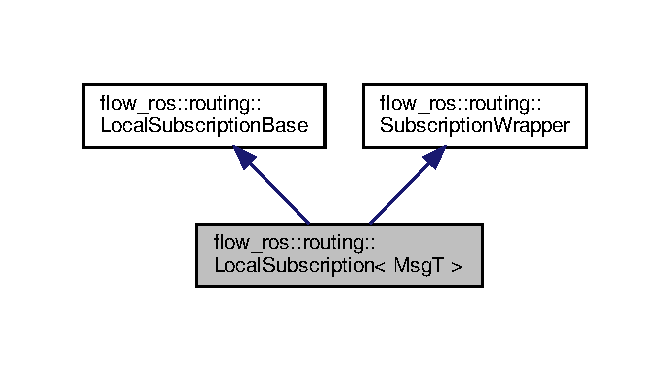
\includegraphics[width=322pt]{classflow__ros_1_1routing_1_1_local_subscription__inherit__graph}
\end{center}
\end{figure}


Collaboration diagram for flow\+\_\+ros\+:\+:routing\+:\+:Local\+Subscription$<$ MsgT $>$\+:\nopagebreak
\begin{figure}[H]
\begin{center}
\leavevmode
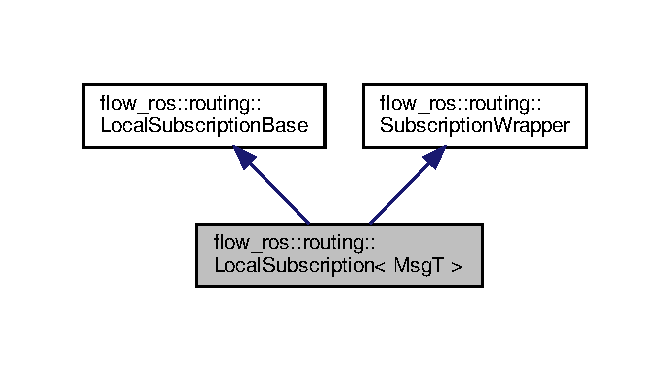
\includegraphics[width=322pt]{classflow__ros_1_1routing_1_1_local_subscription__coll__graph}
\end{center}
\end{figure}
\subsection*{Public Member Functions}
\begin{DoxyCompactItemize}
\item 
{\footnotesize template$<$typename CallbackT $>$ }\\\hyperlink{classflow__ros_1_1routing_1_1_local_subscription_a1237291e8d1b96fc53dfbdd8f03c7b41}{Local\+Subscription} (std\+::string topic, CallbackT \&\&cb)
\begin{DoxyCompactList}\small\item\em Required setup constructor. \end{DoxyCompactList}\item 
\mbox{\Hypertarget{classflow__ros_1_1routing_1_1_local_subscription_a606df699668ffed88b4957647e014369}\label{classflow__ros_1_1routing_1_1_local_subscription_a606df699668ffed88b4957647e014369}} 
virtual \hyperlink{classflow__ros_1_1routing_1_1_local_subscription_a606df699668ffed88b4957647e014369}{$\sim$\+Local\+Subscription} ()=default
\begin{DoxyCompactList}\small\item\em Deconstructor. \end{DoxyCompactList}\item 
void \hyperlink{classflow__ros_1_1routing_1_1_local_subscription_add75c608907362a9e7f808fd15c3ff06}{call} (const \hyperlink{namespaceflow__ros_ad222b6c2bd0341c551129c3a03241ad7}{message\+\_\+shared\+\_\+const\+\_\+ptr\+\_\+t}$<$ MsgT $>$ \&message) const
\begin{DoxyCompactList}\small\item\em Calls subscriber callback with a new message. \end{DoxyCompactList}\item 
void \hyperlink{classflow__ros_1_1routing_1_1_local_subscription_a55ebb76a250f8d45a7fb95d58431c816}{inject} (const \+::rosbag\+::\+Message\+Instance \&mi) const override
\begin{DoxyCompactList}\small\item\em Calls subscriber callback with a rosbag message instance. \end{DoxyCompactList}\item 
std\+::string \hyperlink{classflow__ros_1_1routing_1_1_local_subscription_a24b7dabe9dcabb93339848ae1f8dc57d}{get\+Topic} () const override
\begin{DoxyCompactList}\small\item\em Returns topic associated with publication. \end{DoxyCompactList}\item 
std\+::uint32\+\_\+t \hyperlink{classflow__ros_1_1routing_1_1_local_subscription_a748216bf715060b2435f8e051d547c84}{get\+Num\+Publishers} () const override
\begin{DoxyCompactList}\small\item\em Returns number of local publications connected to this subscription. \end{DoxyCompactList}\item 
\hyperlink{transport__info_8h_ae57afcf849a5bdb82b958347c6ccc57b}{Transport\+Method} \hyperlink{classflow__ros_1_1routing_1_1_local_subscription_a60bf03541b2e5dd1a0af5c80f957f1c1}{get\+Transport\+Method} () const override
\begin{DoxyCompactList}\small\item\em Returns transport method (code) associated with this subscription. \end{DoxyCompactList}\item 
bool \hyperlink{classflow__ros_1_1routing_1_1_local_subscription_ac6fd67afc41be35f69ede7ca5fd8dcfa}{is\+Valid} () const override
\begin{DoxyCompactList}\small\item\em Validity check. \end{DoxyCompactList}\end{DoxyCompactItemize}
\subsection*{Additional Inherited Members}


\subsection{Constructor \& Destructor Documentation}
\mbox{\Hypertarget{classflow__ros_1_1routing_1_1_local_subscription_a1237291e8d1b96fc53dfbdd8f03c7b41}\label{classflow__ros_1_1routing_1_1_local_subscription_a1237291e8d1b96fc53dfbdd8f03c7b41}} 
\index{flow\+\_\+ros\+::routing\+::\+Local\+Subscription@{flow\+\_\+ros\+::routing\+::\+Local\+Subscription}!Local\+Subscription@{Local\+Subscription}}
\index{Local\+Subscription@{Local\+Subscription}!flow\+\_\+ros\+::routing\+::\+Local\+Subscription@{flow\+\_\+ros\+::routing\+::\+Local\+Subscription}}
\subsubsection{\texorpdfstring{Local\+Subscription()}{LocalSubscription()}}
{\footnotesize\ttfamily template$<$typename MsgT $>$ \\
template$<$typename CallbackT $>$ \\
\hyperlink{classflow__ros_1_1routing_1_1_local_subscription}{flow\+\_\+ros\+::routing\+::\+Local\+Subscription}$<$ MsgT $>$\+::\hyperlink{classflow__ros_1_1routing_1_1_local_subscription}{Local\+Subscription} (\begin{DoxyParamCaption}\item[{std\+::string}]{topic,  }\item[{CallbackT \&\&}]{cb }\end{DoxyParamCaption})\hspace{0.3cm}{\ttfamily [inline]}}



Required setup constructor. 


\begin{DoxyParams}{Parameters}
{\em topic} & topic name to associate with this object \\
\hline
{\em cb} & subscriber callback to associate with this object \\
\hline
\end{DoxyParams}


\subsection{Member Function Documentation}
\mbox{\Hypertarget{classflow__ros_1_1routing_1_1_local_subscription_add75c608907362a9e7f808fd15c3ff06}\label{classflow__ros_1_1routing_1_1_local_subscription_add75c608907362a9e7f808fd15c3ff06}} 
\index{flow\+\_\+ros\+::routing\+::\+Local\+Subscription@{flow\+\_\+ros\+::routing\+::\+Local\+Subscription}!call@{call}}
\index{call@{call}!flow\+\_\+ros\+::routing\+::\+Local\+Subscription@{flow\+\_\+ros\+::routing\+::\+Local\+Subscription}}
\subsubsection{\texorpdfstring{call()}{call()}}
{\footnotesize\ttfamily template$<$typename MsgT $>$ \\
void \hyperlink{classflow__ros_1_1routing_1_1_local_subscription}{flow\+\_\+ros\+::routing\+::\+Local\+Subscription}$<$ MsgT $>$\+::call (\begin{DoxyParamCaption}\item[{const \hyperlink{namespaceflow__ros_ad222b6c2bd0341c551129c3a03241ad7}{message\+\_\+shared\+\_\+const\+\_\+ptr\+\_\+t}$<$ MsgT $>$ \&}]{message }\end{DoxyParamCaption}) const\hspace{0.3cm}{\ttfamily [inline]}}



Calls subscriber callback with a new message. 


\begin{DoxyParams}{Parameters}
{\em message} & message data \\
\hline
\end{DoxyParams}
\mbox{\Hypertarget{classflow__ros_1_1routing_1_1_local_subscription_a748216bf715060b2435f8e051d547c84}\label{classflow__ros_1_1routing_1_1_local_subscription_a748216bf715060b2435f8e051d547c84}} 
\index{flow\+\_\+ros\+::routing\+::\+Local\+Subscription@{flow\+\_\+ros\+::routing\+::\+Local\+Subscription}!get\+Num\+Publishers@{get\+Num\+Publishers}}
\index{get\+Num\+Publishers@{get\+Num\+Publishers}!flow\+\_\+ros\+::routing\+::\+Local\+Subscription@{flow\+\_\+ros\+::routing\+::\+Local\+Subscription}}
\subsubsection{\texorpdfstring{get\+Num\+Publishers()}{getNumPublishers()}}
{\footnotesize\ttfamily template$<$typename MsgT $>$ \\
std\+::uint32\+\_\+t \hyperlink{classflow__ros_1_1routing_1_1_local_subscription}{flow\+\_\+ros\+::routing\+::\+Local\+Subscription}$<$ MsgT $>$\+::get\+Num\+Publishers (\begin{DoxyParamCaption}{ }\end{DoxyParamCaption}) const\hspace{0.3cm}{\ttfamily [inline]}, {\ttfamily [override]}, {\ttfamily [virtual]}}



Returns number of local publications connected to this subscription. 



Implements \hyperlink{classflow__ros_1_1routing_1_1_subscription_wrapper_a8ae55d34a07c505dc2b4bcb2440b2d32}{flow\+\_\+ros\+::routing\+::\+Subscription\+Wrapper}.

\mbox{\Hypertarget{classflow__ros_1_1routing_1_1_local_subscription_a24b7dabe9dcabb93339848ae1f8dc57d}\label{classflow__ros_1_1routing_1_1_local_subscription_a24b7dabe9dcabb93339848ae1f8dc57d}} 
\index{flow\+\_\+ros\+::routing\+::\+Local\+Subscription@{flow\+\_\+ros\+::routing\+::\+Local\+Subscription}!get\+Topic@{get\+Topic}}
\index{get\+Topic@{get\+Topic}!flow\+\_\+ros\+::routing\+::\+Local\+Subscription@{flow\+\_\+ros\+::routing\+::\+Local\+Subscription}}
\subsubsection{\texorpdfstring{get\+Topic()}{getTopic()}}
{\footnotesize\ttfamily template$<$typename MsgT $>$ \\
std\+::string \hyperlink{classflow__ros_1_1routing_1_1_local_subscription}{flow\+\_\+ros\+::routing\+::\+Local\+Subscription}$<$ MsgT $>$\+::get\+Topic (\begin{DoxyParamCaption}{ }\end{DoxyParamCaption}) const\hspace{0.3cm}{\ttfamily [inline]}, {\ttfamily [override]}, {\ttfamily [virtual]}}



Returns topic associated with publication. 



Implements \hyperlink{classflow__ros_1_1routing_1_1_subscription_wrapper_a2ef27475e7b7d7555e90d02cdc220b88}{flow\+\_\+ros\+::routing\+::\+Subscription\+Wrapper}.

\mbox{\Hypertarget{classflow__ros_1_1routing_1_1_local_subscription_a60bf03541b2e5dd1a0af5c80f957f1c1}\label{classflow__ros_1_1routing_1_1_local_subscription_a60bf03541b2e5dd1a0af5c80f957f1c1}} 
\index{flow\+\_\+ros\+::routing\+::\+Local\+Subscription@{flow\+\_\+ros\+::routing\+::\+Local\+Subscription}!get\+Transport\+Method@{get\+Transport\+Method}}
\index{get\+Transport\+Method@{get\+Transport\+Method}!flow\+\_\+ros\+::routing\+::\+Local\+Subscription@{flow\+\_\+ros\+::routing\+::\+Local\+Subscription}}
\subsubsection{\texorpdfstring{get\+Transport\+Method()}{getTransportMethod()}}
{\footnotesize\ttfamily template$<$typename MsgT $>$ \\
\hyperlink{transport__info_8h_ae57afcf849a5bdb82b958347c6ccc57b}{Transport\+Method} \hyperlink{classflow__ros_1_1routing_1_1_local_subscription}{flow\+\_\+ros\+::routing\+::\+Local\+Subscription}$<$ MsgT $>$\+::get\+Transport\+Method (\begin{DoxyParamCaption}{ }\end{DoxyParamCaption}) const\hspace{0.3cm}{\ttfamily [inline]}, {\ttfamily [override]}, {\ttfamily [virtual]}}



Returns transport method (code) associated with this subscription. 



Implements \hyperlink{classflow__ros_1_1routing_1_1_subscription_wrapper_a063fcc10600ef657620e2b58ce1fca85}{flow\+\_\+ros\+::routing\+::\+Subscription\+Wrapper}.

\mbox{\Hypertarget{classflow__ros_1_1routing_1_1_local_subscription_a55ebb76a250f8d45a7fb95d58431c816}\label{classflow__ros_1_1routing_1_1_local_subscription_a55ebb76a250f8d45a7fb95d58431c816}} 
\index{flow\+\_\+ros\+::routing\+::\+Local\+Subscription@{flow\+\_\+ros\+::routing\+::\+Local\+Subscription}!inject@{inject}}
\index{inject@{inject}!flow\+\_\+ros\+::routing\+::\+Local\+Subscription@{flow\+\_\+ros\+::routing\+::\+Local\+Subscription}}
\subsubsection{\texorpdfstring{inject()}{inject()}}
{\footnotesize\ttfamily template$<$typename MsgT $>$ \\
void \hyperlink{classflow__ros_1_1routing_1_1_local_subscription}{flow\+\_\+ros\+::routing\+::\+Local\+Subscription}$<$ MsgT $>$\+::inject (\begin{DoxyParamCaption}\item[{const \+::rosbag\+::\+Message\+Instance \&}]{mi }\end{DoxyParamCaption}) const\hspace{0.3cm}{\ttfamily [inline]}, {\ttfamily [override]}, {\ttfamily [virtual]}}



Calls subscriber callback with a rosbag message instance. 


\begin{DoxyParams}{Parameters}
{\em mi} & R\+OS bag message instance\\
\hline
\end{DoxyParams}

\begin{DoxyExceptions}{Exceptions}
{\em $<$code$>$std\+::runtime\+\_\+error$<$/code$>$} & on failure to instance message \\
\hline
\end{DoxyExceptions}
\begin{DoxyNote}{Note}
participates in overload resolution if {\ttfamily MsgT} is a R\+OS message 
\end{DoxyNote}


Implements \hyperlink{classflow__ros_1_1routing_1_1_local_subscription_base_aa2742e8cb1bd70ed0fd6fab679853a7c}{flow\+\_\+ros\+::routing\+::\+Local\+Subscription\+Base}.

\mbox{\Hypertarget{classflow__ros_1_1routing_1_1_local_subscription_ac6fd67afc41be35f69ede7ca5fd8dcfa}\label{classflow__ros_1_1routing_1_1_local_subscription_ac6fd67afc41be35f69ede7ca5fd8dcfa}} 
\index{flow\+\_\+ros\+::routing\+::\+Local\+Subscription@{flow\+\_\+ros\+::routing\+::\+Local\+Subscription}!is\+Valid@{is\+Valid}}
\index{is\+Valid@{is\+Valid}!flow\+\_\+ros\+::routing\+::\+Local\+Subscription@{flow\+\_\+ros\+::routing\+::\+Local\+Subscription}}
\subsubsection{\texorpdfstring{is\+Valid()}{isValid()}}
{\footnotesize\ttfamily template$<$typename MsgT $>$ \\
bool \hyperlink{classflow__ros_1_1routing_1_1_local_subscription}{flow\+\_\+ros\+::routing\+::\+Local\+Subscription}$<$ MsgT $>$\+::is\+Valid (\begin{DoxyParamCaption}{ }\end{DoxyParamCaption}) const\hspace{0.3cm}{\ttfamily [inline]}, {\ttfamily [override]}, {\ttfamily [virtual]}}



Validity check. 


\begin{DoxyRetVals}{Return values}
{\em true} & if a callback has been registered to this object \\
\hline
{\em false} & otherwise \\
\hline
\end{DoxyRetVals}


Implements \hyperlink{classflow__ros_1_1routing_1_1_subscription_wrapper_a0f23052807c3533d28168d7c681a221e}{flow\+\_\+ros\+::routing\+::\+Subscription\+Wrapper}.



The documentation for this class was generated from the following file\+:\begin{DoxyCompactItemize}
\item 
flow\+\_\+ros/include/routing/\hyperlink{local__subscription_8h}{local\+\_\+subscription.\+h}\end{DoxyCompactItemize}

\hypertarget{classflow__ros_1_1routing_1_1_local_subscription_base}{}\section{flow\+\_\+ros\+:\+:routing\+:\+:Local\+Subscription\+Base Class Reference}
\label{classflow__ros_1_1routing_1_1_local_subscription_base}\index{flow\+\_\+ros\+::routing\+::\+Local\+Subscription\+Base@{flow\+\_\+ros\+::routing\+::\+Local\+Subscription\+Base}}


\hyperlink{classflow__ros_1_1routing_1_1_local_subscription}{Local\+Subscription} base which provides basic info and erases Msg\+T-\/dependent methods.  




{\ttfamily \#include $<$local\+\_\+subscription.\+h$>$}



Inheritance diagram for flow\+\_\+ros\+:\+:routing\+:\+:Local\+Subscription\+Base\+:\nopagebreak
\begin{figure}[H]
\begin{center}
\leavevmode
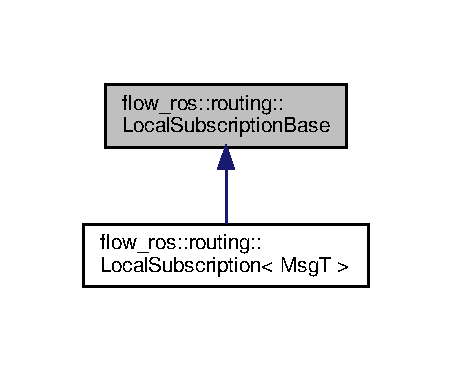
\includegraphics[width=217pt]{classflow__ros_1_1routing_1_1_local_subscription_base__inherit__graph}
\end{center}
\end{figure}
\subsection*{Public Member Functions}
\begin{DoxyCompactItemize}
\item 
\mbox{\Hypertarget{classflow__ros_1_1routing_1_1_local_subscription_base_aa2742e8cb1bd70ed0fd6fab679853a7c}\label{classflow__ros_1_1routing_1_1_local_subscription_base_aa2742e8cb1bd70ed0fd6fab679853a7c}} 
virtual void \hyperlink{classflow__ros_1_1routing_1_1_local_subscription_base_aa2742e8cb1bd70ed0fd6fab679853a7c}{inject} (const \+::rosbag\+::\+Message\+Instance \&mi) const =0
\begin{DoxyCompactList}\small\item\em Calls subscriber callback with a rosbag message instance. \end{DoxyCompactList}\end{DoxyCompactItemize}


\subsection{Detailed Description}
\hyperlink{classflow__ros_1_1routing_1_1_local_subscription}{Local\+Subscription} base which provides basic info and erases Msg\+T-\/dependent methods. 

The documentation for this class was generated from the following file\+:\begin{DoxyCompactItemize}
\item 
flow\+\_\+ros/include/routing/\hyperlink{local__subscription_8h}{local\+\_\+subscription.\+h}\end{DoxyCompactItemize}

\hypertarget{classflow__ros_1_1routing_1_1_local_subscription_group}{}\section{flow\+\_\+ros\+:\+:routing\+:\+:Local\+Subscription\+Group Class Reference}
\label{classflow__ros_1_1routing_1_1_local_subscription_group}\index{flow\+\_\+ros\+::routing\+::\+Local\+Subscription\+Group@{flow\+\_\+ros\+::routing\+::\+Local\+Subscription\+Group}}


Holds a group of \hyperlink{classflow__ros_1_1routing_1_1_local_subscription}{Local\+Subscription} objects associated with a particular topic.  




{\ttfamily \#include $<$local\+\_\+subscription.\+h$>$}

\subsection*{Public Member Functions}
\begin{DoxyCompactItemize}
\item 
{\footnotesize template$<$typename MsgT $>$ }\\void \hyperlink{classflow__ros_1_1routing_1_1_local_subscription_group_af8ee0436491f90218fd94b088dd170ee}{call} (const \hyperlink{namespaceflow__ros_ad222b6c2bd0341c551129c3a03241ad7}{message\+\_\+shared\+\_\+const\+\_\+ptr\+\_\+t}$<$ MsgT $>$ \&message) const
\begin{DoxyCompactList}\small\item\em Calls all subscriber callbacks on a new message. \end{DoxyCompactList}\item 
void \hyperlink{classflow__ros_1_1routing_1_1_local_subscription_group_a2ec4b4ade12601eaf36e9ffbee113100}{inject} (const \+::rosbag\+::\+Message\+Instance \&mi) const
\begin{DoxyCompactList}\small\item\em Calls subscriber callback with a rosbag message instance. \end{DoxyCompactList}\item 
{\footnotesize template$<$typename MsgT $>$ }\\void \hyperlink{classflow__ros_1_1routing_1_1_local_subscription_group_ab6feb50cfaff51aae2b06da8b95a355a}{add\+Subscription} (std\+::shared\+\_\+ptr$<$ \hyperlink{classflow__ros_1_1routing_1_1_local_subscription}{Local\+Subscription}$<$ MsgT $>$$>$ sub)
\begin{DoxyCompactList}\small\item\em Adds new subscriptions to group. \end{DoxyCompactList}\item 
\hyperlink{classflow__ros_1_1routing_1_1_local_subscription_group_aa63f6c379889d06a99c118d2dc9cdb67}{operator bool} () const
\begin{DoxyCompactList}\small\item\em Validation cast operator. \end{DoxyCompactList}\item 
\mbox{\Hypertarget{classflow__ros_1_1routing_1_1_local_subscription_group_a4a8df5ea6c5c4e2a6f961e8d9bb626cf}\label{classflow__ros_1_1routing_1_1_local_subscription_group_a4a8df5ea6c5c4e2a6f961e8d9bb626cf}} 
std\+::size\+\_\+t \hyperlink{classflow__ros_1_1routing_1_1_local_subscription_group_a4a8df5ea6c5c4e2a6f961e8d9bb626cf}{size} () const
\begin{DoxyCompactList}\small\item\em Returns the number of held subscriptions. \end{DoxyCompactList}\end{DoxyCompactItemize}


\subsection{Detailed Description}
Holds a group of \hyperlink{classflow__ros_1_1routing_1_1_local_subscription}{Local\+Subscription} objects associated with a particular topic. 

\subsection{Member Function Documentation}
\mbox{\Hypertarget{classflow__ros_1_1routing_1_1_local_subscription_group_ab6feb50cfaff51aae2b06da8b95a355a}\label{classflow__ros_1_1routing_1_1_local_subscription_group_ab6feb50cfaff51aae2b06da8b95a355a}} 
\index{flow\+\_\+ros\+::routing\+::\+Local\+Subscription\+Group@{flow\+\_\+ros\+::routing\+::\+Local\+Subscription\+Group}!add\+Subscription@{add\+Subscription}}
\index{add\+Subscription@{add\+Subscription}!flow\+\_\+ros\+::routing\+::\+Local\+Subscription\+Group@{flow\+\_\+ros\+::routing\+::\+Local\+Subscription\+Group}}
\subsubsection{\texorpdfstring{add\+Subscription()}{addSubscription()}}
{\footnotesize\ttfamily template$<$typename MsgT $>$ \\
void flow\+\_\+ros\+::routing\+::\+Local\+Subscription\+Group\+::add\+Subscription (\begin{DoxyParamCaption}\item[{std\+::shared\+\_\+ptr$<$ \hyperlink{classflow__ros_1_1routing_1_1_local_subscription}{Local\+Subscription}$<$ MsgT $>$$>$}]{sub }\end{DoxyParamCaption})\hspace{0.3cm}{\ttfamily [inline]}}



Adds new subscriptions to group. 


\begin{DoxyParams}{Parameters}
{\em sub} & \hyperlink{classflow__ros_1_1routing_1_1_local_subscription}{Local\+Subscription} resource \\
\hline
\end{DoxyParams}
\mbox{\Hypertarget{classflow__ros_1_1routing_1_1_local_subscription_group_af8ee0436491f90218fd94b088dd170ee}\label{classflow__ros_1_1routing_1_1_local_subscription_group_af8ee0436491f90218fd94b088dd170ee}} 
\index{flow\+\_\+ros\+::routing\+::\+Local\+Subscription\+Group@{flow\+\_\+ros\+::routing\+::\+Local\+Subscription\+Group}!call@{call}}
\index{call@{call}!flow\+\_\+ros\+::routing\+::\+Local\+Subscription\+Group@{flow\+\_\+ros\+::routing\+::\+Local\+Subscription\+Group}}
\subsubsection{\texorpdfstring{call()}{call()}}
{\footnotesize\ttfamily template$<$typename MsgT $>$ \\
void flow\+\_\+ros\+::routing\+::\+Local\+Subscription\+Group\+::call (\begin{DoxyParamCaption}\item[{const \hyperlink{namespaceflow__ros_ad222b6c2bd0341c551129c3a03241ad7}{message\+\_\+shared\+\_\+const\+\_\+ptr\+\_\+t}$<$ MsgT $>$ \&}]{message }\end{DoxyParamCaption}) const\hspace{0.3cm}{\ttfamily [inline]}}



Calls all subscriber callbacks on a new message. 


\begin{DoxyParams}{Parameters}
{\em message} & message data\\
\hline
\end{DoxyParams}

\begin{DoxyExceptions}{Exceptions}
{\em $<$code$>$\+Message\+Type\+Error$<$/code$>$} & if {\ttfamily MsgT} is incompatible with subscription group \\
\hline
\end{DoxyExceptions}
\mbox{\Hypertarget{classflow__ros_1_1routing_1_1_local_subscription_group_a2ec4b4ade12601eaf36e9ffbee113100}\label{classflow__ros_1_1routing_1_1_local_subscription_group_a2ec4b4ade12601eaf36e9ffbee113100}} 
\index{flow\+\_\+ros\+::routing\+::\+Local\+Subscription\+Group@{flow\+\_\+ros\+::routing\+::\+Local\+Subscription\+Group}!inject@{inject}}
\index{inject@{inject}!flow\+\_\+ros\+::routing\+::\+Local\+Subscription\+Group@{flow\+\_\+ros\+::routing\+::\+Local\+Subscription\+Group}}
\subsubsection{\texorpdfstring{inject()}{inject()}}
{\footnotesize\ttfamily void flow\+\_\+ros\+::routing\+::\+Local\+Subscription\+Group\+::inject (\begin{DoxyParamCaption}\item[{const \+::rosbag\+::\+Message\+Instance \&}]{mi }\end{DoxyParamCaption}) const\hspace{0.3cm}{\ttfamily [inline]}}



Calls subscriber callback with a rosbag message instance. 


\begin{DoxyParams}{Parameters}
{\em mi} & R\+OS bag message instance \\
\hline
\end{DoxyParams}
\mbox{\Hypertarget{classflow__ros_1_1routing_1_1_local_subscription_group_aa63f6c379889d06a99c118d2dc9cdb67}\label{classflow__ros_1_1routing_1_1_local_subscription_group_aa63f6c379889d06a99c118d2dc9cdb67}} 
\index{flow\+\_\+ros\+::routing\+::\+Local\+Subscription\+Group@{flow\+\_\+ros\+::routing\+::\+Local\+Subscription\+Group}!operator bool@{operator bool}}
\index{operator bool@{operator bool}!flow\+\_\+ros\+::routing\+::\+Local\+Subscription\+Group@{flow\+\_\+ros\+::routing\+::\+Local\+Subscription\+Group}}
\subsubsection{\texorpdfstring{operator bool()}{operator bool()}}
{\footnotesize\ttfamily flow\+\_\+ros\+::routing\+::\+Local\+Subscription\+Group\+::operator bool (\begin{DoxyParamCaption}{ }\end{DoxyParamCaption}) const\hspace{0.3cm}{\ttfamily [inline]}}



Validation cast operator. 


\begin{DoxyRetVals}{Return values}
{\em true} & if there are any held subscriptions \\
\hline
{\em false} & otherwise \\
\hline
\end{DoxyRetVals}


The documentation for this class was generated from the following file\+:\begin{DoxyCompactItemize}
\item 
flow\+\_\+ros/include/routing/\hyperlink{local__subscription_8h}{local\+\_\+subscription.\+h}\end{DoxyCompactItemize}

\hypertarget{classflow__ros_1_1routing_1_1_message_instance_error}{}\section{flow\+\_\+ros\+:\+:routing\+:\+:Message\+Instance\+Error Class Reference}
\label{classflow__ros_1_1routing_1_1_message_instance_error}\index{flow\+\_\+ros\+::routing\+::\+Message\+Instance\+Error@{flow\+\_\+ros\+::routing\+::\+Message\+Instance\+Error}}


Exception thrown when a message cannot be instanced from {\ttfamily rosbag\+::\+Message\+Instance}  




{\ttfamily \#include $<$local\+\_\+subscription.\+h$>$}



Inheritance diagram for flow\+\_\+ros\+:\+:routing\+:\+:Message\+Instance\+Error\+:\nopagebreak
\begin{figure}[H]
\begin{center}
\leavevmode
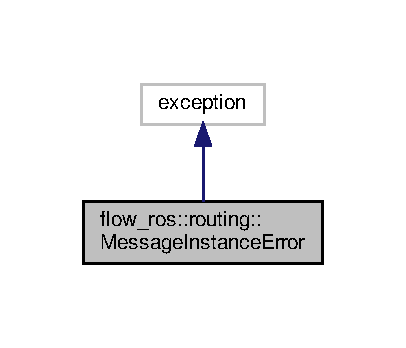
\includegraphics[width=195pt]{classflow__ros_1_1routing_1_1_message_instance_error__inherit__graph}
\end{center}
\end{figure}


Collaboration diagram for flow\+\_\+ros\+:\+:routing\+:\+:Message\+Instance\+Error\+:\nopagebreak
\begin{figure}[H]
\begin{center}
\leavevmode
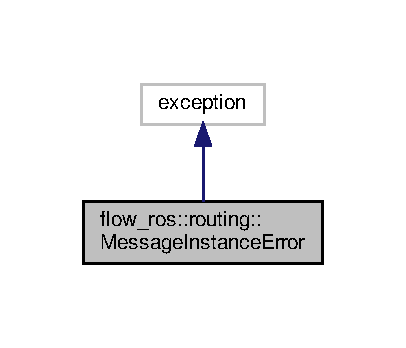
\includegraphics[width=195pt]{classflow__ros_1_1routing_1_1_message_instance_error__coll__graph}
\end{center}
\end{figure}
\subsection*{Public Member Functions}
\begin{DoxyCompactItemize}
\item 
\mbox{\Hypertarget{classflow__ros_1_1routing_1_1_message_instance_error_a7e9b4e5df423450b855256bfcbea2b6f}\label{classflow__ros_1_1routing_1_1_message_instance_error_a7e9b4e5df423450b855256bfcbea2b6f}} 
{\footnotesize template$<$typename StringT $>$ }\\{\bfseries Message\+Instance\+Error} (StringT \&\&what)
\item 
\mbox{\Hypertarget{classflow__ros_1_1routing_1_1_message_instance_error_a944235334f1dd42384d724dce8e51430}\label{classflow__ros_1_1routing_1_1_message_instance_error_a944235334f1dd42384d724dce8e51430}} 
const char $\ast$ {\bfseries what} () const noexcept
\end{DoxyCompactItemize}


\subsection{Detailed Description}
Exception thrown when a message cannot be instanced from {\ttfamily rosbag\+::\+Message\+Instance} 

The documentation for this class was generated from the following file\+:\begin{DoxyCompactItemize}
\item 
flow\+\_\+ros/include/routing/\hyperlink{local__subscription_8h}{local\+\_\+subscription.\+h}\end{DoxyCompactItemize}

\hypertarget{structflow__ros_1_1_message_shared_const_ptr_type}{}\section{flow\+\_\+ros\+:\+:Message\+Shared\+Const\+Ptr\+Type$<$ MsgT, I\+S\+\_\+\+R\+O\+S\+\_\+\+M\+E\+S\+S\+A\+GE $>$ Struct Template Reference}
\label{structflow__ros_1_1_message_shared_const_ptr_type}\index{flow\+\_\+ros\+::\+Message\+Shared\+Const\+Ptr\+Type$<$ Msg\+T, I\+S\+\_\+\+R\+O\+S\+\_\+\+M\+E\+S\+S\+A\+G\+E $>$@{flow\+\_\+ros\+::\+Message\+Shared\+Const\+Ptr\+Type$<$ Msg\+T, I\+S\+\_\+\+R\+O\+S\+\_\+\+M\+E\+S\+S\+A\+G\+E $>$}}


Traits object used to select correct shared\+\_\+ptr const resource wrapper.  




{\ttfamily \#include $<$message\+\_\+ptr.\+h$>$}

\subsection*{Public Types}
\begin{DoxyCompactItemize}
\item 
\mbox{\Hypertarget{structflow__ros_1_1_message_shared_const_ptr_type_aa54b6baec54b3a19815aa429b42ae97c}\label{structflow__ros_1_1_message_shared_const_ptr_type_aa54b6baec54b3a19815aa429b42ae97c}} 
using {\bfseries type} = \hyperlink{namespaceflow__ros_aa27be896eb2c4c34fef0e9b7dd444d4c}{non\+\_\+message\+\_\+shared\+\_\+ptr\+\_\+t}$<$ const std\+::remove\+\_\+const\+\_\+t$<$ MsgT $>$ $>$
\end{DoxyCompactItemize}


\subsection{Detailed Description}
\subsubsection*{template$<$typename MsgT, bool I\+S\+\_\+\+R\+O\+S\+\_\+\+M\+E\+S\+S\+A\+GE = is\+\_\+message\+\_\+v$<$\+Msg\+T$>$$>$\newline
struct flow\+\_\+ros\+::\+Message\+Shared\+Const\+Ptr\+Type$<$ Msg\+T, I\+S\+\_\+\+R\+O\+S\+\_\+\+M\+E\+S\+S\+A\+G\+E $>$}

Traits object used to select correct shared\+\_\+ptr const resource wrapper. 


\begin{DoxyTemplParams}{Template Parameters}
{\em MsgT} & message type \\
\hline
{\em I\+S\+\_\+\+R\+O\+S\+\_\+\+M\+E\+S\+S\+A\+GE} & \mbox{[}DO N\+OT S\+U\+P\+P\+LY T\+H\+IS A\+R\+G\+U\+M\+E\+NT\mbox{]} (defaulted) to see if MsgT is a R\+OS message \\
\hline
\end{DoxyTemplParams}


The documentation for this struct was generated from the following file\+:\begin{DoxyCompactItemize}
\item 
flow\+\_\+ros/include/\hyperlink{message__ptr_8h}{message\+\_\+ptr.\+h}\end{DoxyCompactItemize}

\hypertarget{structflow__ros_1_1_message_shared_const_ptr_type_3_01_msg_t_00_01true_01_4}{}\section{flow\+\_\+ros\+:\+:Message\+Shared\+Const\+Ptr\+Type$<$ MsgT, true $>$ Struct Template Reference}
\label{structflow__ros_1_1_message_shared_const_ptr_type_3_01_msg_t_00_01true_01_4}\index{flow\+\_\+ros\+::\+Message\+Shared\+Const\+Ptr\+Type$<$ Msg\+T, true $>$@{flow\+\_\+ros\+::\+Message\+Shared\+Const\+Ptr\+Type$<$ Msg\+T, true $>$}}


Traits object used to select correct shared\+\_\+ptr const resource wrapper.  




{\ttfamily \#include $<$message\+\_\+ptr.\+h$>$}

\subsection*{Public Types}
\begin{DoxyCompactItemize}
\item 
\mbox{\Hypertarget{structflow__ros_1_1_message_shared_const_ptr_type_3_01_msg_t_00_01true_01_4_a9e1cf8f521bb65087550c9c9c1c7f5fd}\label{structflow__ros_1_1_message_shared_const_ptr_type_3_01_msg_t_00_01true_01_4_a9e1cf8f521bb65087550c9c9c1c7f5fd}} 
using {\bfseries type} = boost\+::shared\+\_\+ptr$<$ const std\+::remove\+\_\+const\+\_\+t$<$ MsgT $>$ $>$
\end{DoxyCompactItemize}


\subsection{Detailed Description}
\subsubsection*{template$<$typename MsgT$>$\newline
struct flow\+\_\+ros\+::\+Message\+Shared\+Const\+Ptr\+Type$<$ Msg\+T, true $>$}

Traits object used to select correct shared\+\_\+ptr const resource wrapper. 


\begin{DoxyTemplParams}{Template Parameters}
{\em MsgT} & message type \\
\hline
{\em I\+S\+\_\+\+R\+O\+S\+\_\+\+M\+E\+S\+S\+A\+GE} & \mbox{[}DO N\+OT S\+U\+P\+P\+LY T\+H\+IS A\+R\+G\+U\+M\+E\+NT\mbox{]} (defaulted) to see if MsgT is a R\+OS message \\
\hline
\end{DoxyTemplParams}
\begin{DoxyNote}{Note}
Specialization for R\+OS messages 
\end{DoxyNote}


The documentation for this struct was generated from the following file\+:\begin{DoxyCompactItemize}
\item 
flow\+\_\+ros/include/\hyperlink{message__ptr_8h}{message\+\_\+ptr.\+h}\end{DoxyCompactItemize}

\hypertarget{structflow__ros_1_1_message_shared_ptr_type}{}\section{flow\+\_\+ros\+:\+:Message\+Shared\+Ptr\+Type$<$ MsgT, I\+S\+\_\+\+R\+O\+S\+\_\+\+M\+E\+S\+S\+A\+GE $>$ Struct Template Reference}
\label{structflow__ros_1_1_message_shared_ptr_type}\index{flow\+\_\+ros\+::\+Message\+Shared\+Ptr\+Type$<$ Msg\+T, I\+S\+\_\+\+R\+O\+S\+\_\+\+M\+E\+S\+S\+A\+G\+E $>$@{flow\+\_\+ros\+::\+Message\+Shared\+Ptr\+Type$<$ Msg\+T, I\+S\+\_\+\+R\+O\+S\+\_\+\+M\+E\+S\+S\+A\+G\+E $>$}}


Traits object used to select correct shared\+\_\+ptr resource type.  




{\ttfamily \#include $<$message\+\_\+ptr.\+h$>$}

\subsection*{Public Types}
\begin{DoxyCompactItemize}
\item 
\mbox{\Hypertarget{structflow__ros_1_1_message_shared_ptr_type_aa79edee80bae6b91f849accaf772c92b}\label{structflow__ros_1_1_message_shared_ptr_type_aa79edee80bae6b91f849accaf772c92b}} 
using {\bfseries type} = \hyperlink{namespaceflow__ros_aa27be896eb2c4c34fef0e9b7dd444d4c}{non\+\_\+message\+\_\+shared\+\_\+ptr\+\_\+t}$<$ MsgT $>$
\end{DoxyCompactItemize}


\subsection{Detailed Description}
\subsubsection*{template$<$typename MsgT, bool I\+S\+\_\+\+R\+O\+S\+\_\+\+M\+E\+S\+S\+A\+GE = is\+\_\+message\+\_\+v$<$\+Msg\+T$>$$>$\newline
struct flow\+\_\+ros\+::\+Message\+Shared\+Ptr\+Type$<$ Msg\+T, I\+S\+\_\+\+R\+O\+S\+\_\+\+M\+E\+S\+S\+A\+G\+E $>$}

Traits object used to select correct shared\+\_\+ptr resource type. 


\begin{DoxyTemplParams}{Template Parameters}
{\em MsgT} & message type \\
\hline
{\em I\+S\+\_\+\+R\+O\+S\+\_\+\+M\+E\+S\+S\+A\+GE} & \mbox{[}DO N\+OT S\+U\+P\+P\+LY T\+H\+IS A\+R\+G\+U\+M\+E\+NT\mbox{]} (defaulted) to see if MsgT is a R\+OS message \\
\hline
\end{DoxyTemplParams}


The documentation for this struct was generated from the following file\+:\begin{DoxyCompactItemize}
\item 
flow\+\_\+ros/include/\hyperlink{message__ptr_8h}{message\+\_\+ptr.\+h}\end{DoxyCompactItemize}

\hypertarget{structflow__ros_1_1_message_shared_ptr_type_3_01_msg_t_00_01true_01_4}{}\section{flow\+\_\+ros\+:\+:Message\+Shared\+Ptr\+Type$<$ MsgT, true $>$ Struct Template Reference}
\label{structflow__ros_1_1_message_shared_ptr_type_3_01_msg_t_00_01true_01_4}\index{flow\+\_\+ros\+::\+Message\+Shared\+Ptr\+Type$<$ Msg\+T, true $>$@{flow\+\_\+ros\+::\+Message\+Shared\+Ptr\+Type$<$ Msg\+T, true $>$}}


Traits object used to select correct shared\+\_\+ptr resource type.  




{\ttfamily \#include $<$message\+\_\+ptr.\+h$>$}

\subsection*{Public Types}
\begin{DoxyCompactItemize}
\item 
\mbox{\Hypertarget{structflow__ros_1_1_message_shared_ptr_type_3_01_msg_t_00_01true_01_4_a748eb553b42c2c7b1acdcc09c04c1c83}\label{structflow__ros_1_1_message_shared_ptr_type_3_01_msg_t_00_01true_01_4_a748eb553b42c2c7b1acdcc09c04c1c83}} 
using {\bfseries type} = boost\+::shared\+\_\+ptr$<$ MsgT $>$
\end{DoxyCompactItemize}


\subsection{Detailed Description}
\subsubsection*{template$<$typename MsgT$>$\newline
struct flow\+\_\+ros\+::\+Message\+Shared\+Ptr\+Type$<$ Msg\+T, true $>$}

Traits object used to select correct shared\+\_\+ptr resource type. 


\begin{DoxyTemplParams}{Template Parameters}
{\em MsgT} & message type \\
\hline
{\em I\+S\+\_\+\+R\+O\+S\+\_\+\+M\+E\+S\+S\+A\+GE} & \mbox{[}DO N\+OT S\+U\+P\+P\+LY T\+H\+IS A\+R\+G\+U\+M\+E\+NT\mbox{]} (defaulted) to see if MsgT is a R\+OS message \\
\hline
\end{DoxyTemplParams}
\begin{DoxyNote}{Note}
Specialization for R\+OS messages 
\end{DoxyNote}


The documentation for this struct was generated from the following file\+:\begin{DoxyCompactItemize}
\item 
flow\+\_\+ros/include/\hyperlink{message__ptr_8h}{message\+\_\+ptr.\+h}\end{DoxyCompactItemize}

\hypertarget{classflow__ros_1_1routing_1_1_message_type_error}{}\section{flow\+\_\+ros\+:\+:routing\+:\+:Message\+Type\+Error Class Reference}
\label{classflow__ros_1_1routing_1_1_message_type_error}\index{flow\+\_\+ros\+::routing\+::\+Message\+Type\+Error@{flow\+\_\+ros\+::routing\+::\+Message\+Type\+Error}}


Exception thrown when a message type does not match for a given topic.  




{\ttfamily \#include $<$local\+\_\+subscription.\+h$>$}



Inheritance diagram for flow\+\_\+ros\+:\+:routing\+:\+:Message\+Type\+Error\+:\nopagebreak
\begin{figure}[H]
\begin{center}
\leavevmode
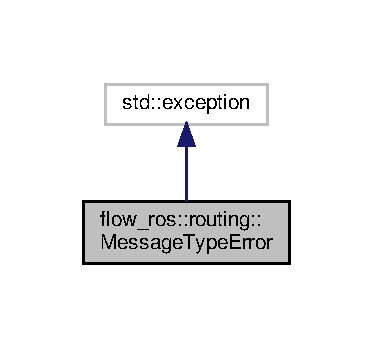
\includegraphics[width=179pt]{classflow__ros_1_1routing_1_1_message_type_error__inherit__graph}
\end{center}
\end{figure}


Collaboration diagram for flow\+\_\+ros\+:\+:routing\+:\+:Message\+Type\+Error\+:\nopagebreak
\begin{figure}[H]
\begin{center}
\leavevmode
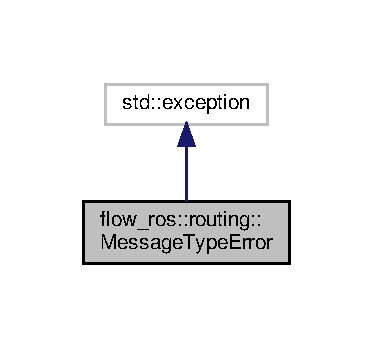
\includegraphics[width=179pt]{classflow__ros_1_1routing_1_1_message_type_error__coll__graph}
\end{center}
\end{figure}
\subsection*{Public Member Functions}
\begin{DoxyCompactItemize}
\item 
\mbox{\Hypertarget{classflow__ros_1_1routing_1_1_message_type_error_ab9665e2b6000e0db3d5bbfcba7abf42b}\label{classflow__ros_1_1routing_1_1_message_type_error_ab9665e2b6000e0db3d5bbfcba7abf42b}} 
{\footnotesize template$<$typename StringT $>$ }\\{\bfseries Message\+Type\+Error} (StringT \&\&what)
\item 
\mbox{\Hypertarget{classflow__ros_1_1routing_1_1_message_type_error_a3cce8f2383902caa8f6254d25554d89b}\label{classflow__ros_1_1routing_1_1_message_type_error_a3cce8f2383902caa8f6254d25554d89b}} 
const char $\ast$ {\bfseries what} () const noexcept
\end{DoxyCompactItemize}


\subsection{Detailed Description}
Exception thrown when a message type does not match for a given topic. 

The documentation for this class was generated from the following file\+:\begin{DoxyCompactItemize}
\item 
flow\+\_\+ros/include/routing/\hyperlink{local__subscription_8h}{local\+\_\+subscription.\+h}\end{DoxyCompactItemize}

\hypertarget{classflow__ros_1_1_multi_publisher}{}\section{flow\+\_\+ros\+:\+:Multi\+Publisher$<$ MsgT, Output\+ContainerT $>$ Class Template Reference}
\label{classflow__ros_1_1_multi_publisher}\index{flow\+\_\+ros\+::\+Multi\+Publisher$<$ Msg\+T, Output\+Container\+T $>$@{flow\+\_\+ros\+::\+Multi\+Publisher$<$ Msg\+T, Output\+Container\+T $>$}}


Output channel specialization which publishes multiple messages.  




{\ttfamily \#include $<$publisher.\+h$>$}



Inheritance diagram for flow\+\_\+ros\+:\+:Multi\+Publisher$<$ MsgT, Output\+ContainerT $>$\+:\nopagebreak
\begin{figure}[H]
\begin{center}
\leavevmode
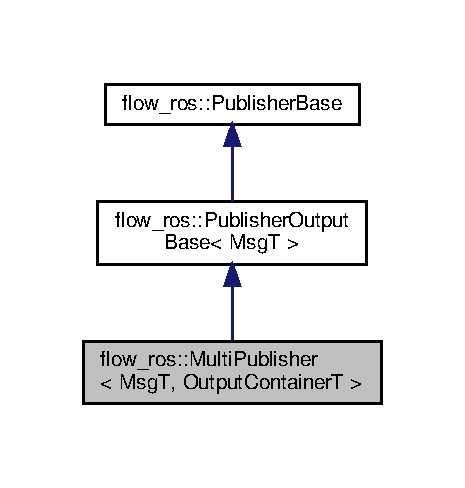
\includegraphics[width=223pt]{classflow__ros_1_1_multi_publisher__inherit__graph}
\end{center}
\end{figure}


Collaboration diagram for flow\+\_\+ros\+:\+:Multi\+Publisher$<$ MsgT, Output\+ContainerT $>$\+:\nopagebreak
\begin{figure}[H]
\begin{center}
\leavevmode
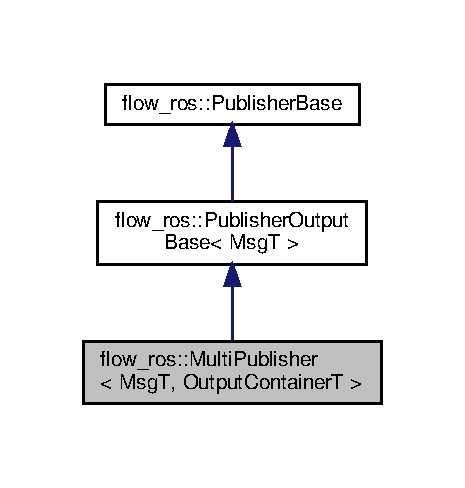
\includegraphics[width=223pt]{classflow__ros_1_1_multi_publisher__coll__graph}
\end{center}
\end{figure}
\subsection*{Public Member Functions}
\begin{DoxyCompactItemize}
\item 
\mbox{\Hypertarget{classflow__ros_1_1_multi_publisher_a4bf4647962d3dcd52e3c89549f9abceb}\label{classflow__ros_1_1_multi_publisher_a4bf4647962d3dcd52e3c89549f9abceb}} 
{\bfseries F\+L\+O\+W\+\_\+\+S\+T\+A\+T\+I\+C\+\_\+\+A\+S\+S\+E\+RT} (std\+::is\+\_\+const$<$ MsgT $>$(), \char`\"{}MsgT must be const\char`\"{})
\item 
\hyperlink{classflow__ros_1_1_multi_publisher_a3e2ddbd297bd541cd4c7be71786a4bf0}{Multi\+Publisher} (ros\+::\+Node\+Handle \&nh, const std\+::string \&topic, const std\+::uint32\+\_\+t queue\+\_\+size=0, const bool latched=false)
\begin{DoxyCompactList}\small\item\em {\ttfamily ros\+::\+Node\+Handle} setup constructor (extra-\/node messaging) \end{DoxyCompactList}\item 
\hyperlink{classflow__ros_1_1_multi_publisher_af1d0509e1464ddb1a92e72cc90ed08cd}{Multi\+Publisher} (\hyperlink{classflow__ros_1_1_router}{Router} \&pb, std\+::string topic, const std\+::uint32\+\_\+t queue\+\_\+size=0)
\begin{DoxyCompactList}\small\item\em {\ttfamily \hyperlink{classflow__ros_1_1_router}{Router}} setup constructor (intra-\/node messaging) \end{DoxyCompactList}\item 
{\footnotesize template$<$typename Msg\+Ptr\+IteratorT $>$ }\\void \hyperlink{classflow__ros_1_1_multi_publisher_a639d20b3dd0dbc9598b8e08c0ec84255}{publish} (Msg\+Ptr\+IteratorT first, const Msg\+Ptr\+IteratorT last) const
\begin{DoxyCompactList}\small\item\em Publishes range of messages. \end{DoxyCompactList}\item 
void \hyperlink{classflow__ros_1_1_multi_publisher_adea00fbe1e1b566c9e374105325cbc6c}{publish} (const Output\+ContainerT \&messages) const
\begin{DoxyCompactList}\small\item\em Publishes range of messages. \end{DoxyCompactList}\end{DoxyCompactItemize}
\subsection*{Additional Inherited Members}


\subsection{Detailed Description}
\subsubsection*{template$<$typename MsgT, typename Output\+ContainerT = std\+::vector$<$message\+\_\+shared\+\_\+ptr\+\_\+t$<$\+Msg\+T$>$$>$$>$\newline
class flow\+\_\+ros\+::\+Multi\+Publisher$<$ Msg\+T, Output\+Container\+T $>$}

Output channel specialization which publishes multiple messages. 


\begin{DoxyTemplParams}{Template Parameters}
{\em MsgT} & message type \\
\hline
{\em Output\+ContainerT} & container of message resources used as {\ttfamily Output\+Type}; this information is most relevant when using with \hyperlink{classflow__ros_1_1_multi_publisher}{Multi\+Publisher} with \hyperlink{classflow__ros_1_1_event_handler}{Event\+Handler} \\
\hline
\end{DoxyTemplParams}


\subsection{Constructor \& Destructor Documentation}
\mbox{\Hypertarget{classflow__ros_1_1_multi_publisher_a3e2ddbd297bd541cd4c7be71786a4bf0}\label{classflow__ros_1_1_multi_publisher_a3e2ddbd297bd541cd4c7be71786a4bf0}} 
\index{flow\+\_\+ros\+::\+Multi\+Publisher@{flow\+\_\+ros\+::\+Multi\+Publisher}!Multi\+Publisher@{Multi\+Publisher}}
\index{Multi\+Publisher@{Multi\+Publisher}!flow\+\_\+ros\+::\+Multi\+Publisher@{flow\+\_\+ros\+::\+Multi\+Publisher}}
\subsubsection{\texorpdfstring{Multi\+Publisher()}{MultiPublisher()}\hspace{0.1cm}{\footnotesize\ttfamily [1/2]}}
{\footnotesize\ttfamily template$<$typename MsgT, typename Output\+ContainerT = std\+::vector$<$message\+\_\+shared\+\_\+ptr\+\_\+t$<$\+Msg\+T$>$$>$$>$ \\
\hyperlink{classflow__ros_1_1_multi_publisher}{flow\+\_\+ros\+::\+Multi\+Publisher}$<$ MsgT, Output\+ContainerT $>$\+::\hyperlink{classflow__ros_1_1_multi_publisher}{Multi\+Publisher} (\begin{DoxyParamCaption}\item[{ros\+::\+Node\+Handle \&}]{nh,  }\item[{const std\+::string \&}]{topic,  }\item[{const std\+::uint32\+\_\+t}]{queue\+\_\+size = {\ttfamily 0},  }\item[{const bool}]{latched = {\ttfamily false} }\end{DoxyParamCaption})\hspace{0.3cm}{\ttfamily [inline]}}



{\ttfamily ros\+::\+Node\+Handle} setup constructor (extra-\/node messaging) 


\begin{DoxyParams}[1]{Parameters}
\mbox{\tt in,out}  & {\em nh} & R\+OS node handle to negotiate topic advertisement/connection \\
\hline
 & {\em topic} & topic associated with messages to be output \\
\hline
 & {\em queue\+\_\+size} & underlying R\+OS publisher queue size \\
\hline
 & {\em latched} & options for creating a \char`\"{}latched\char`\"{} output publisher\\
\hline
\end{DoxyParams}
\begin{DoxyWarning}{Warning}
Will throw with {\ttfamily std\+::runtime\+\_\+error} if underlying publisher could not be establish a connection with R\+O\+S-\/master 
\end{DoxyWarning}
\mbox{\Hypertarget{classflow__ros_1_1_multi_publisher_af1d0509e1464ddb1a92e72cc90ed08cd}\label{classflow__ros_1_1_multi_publisher_af1d0509e1464ddb1a92e72cc90ed08cd}} 
\index{flow\+\_\+ros\+::\+Multi\+Publisher@{flow\+\_\+ros\+::\+Multi\+Publisher}!Multi\+Publisher@{Multi\+Publisher}}
\index{Multi\+Publisher@{Multi\+Publisher}!flow\+\_\+ros\+::\+Multi\+Publisher@{flow\+\_\+ros\+::\+Multi\+Publisher}}
\subsubsection{\texorpdfstring{Multi\+Publisher()}{MultiPublisher()}\hspace{0.1cm}{\footnotesize\ttfamily [2/2]}}
{\footnotesize\ttfamily template$<$typename MsgT, typename Output\+ContainerT = std\+::vector$<$message\+\_\+shared\+\_\+ptr\+\_\+t$<$\+Msg\+T$>$$>$$>$ \\
\hyperlink{classflow__ros_1_1_multi_publisher}{flow\+\_\+ros\+::\+Multi\+Publisher}$<$ MsgT, Output\+ContainerT $>$\+::\hyperlink{classflow__ros_1_1_multi_publisher}{Multi\+Publisher} (\begin{DoxyParamCaption}\item[{\hyperlink{classflow__ros_1_1_router}{Router} \&}]{pb,  }\item[{std\+::string}]{topic,  }\item[{const std\+::uint32\+\_\+t}]{queue\+\_\+size = {\ttfamily 0} }\end{DoxyParamCaption})\hspace{0.3cm}{\ttfamily [inline]}}



{\ttfamily \hyperlink{classflow__ros_1_1_router}{Router}} setup constructor (intra-\/node messaging) 


\begin{DoxyParams}[1]{Parameters}
\mbox{\tt in,out}  & {\em pb} & Intra-\/node \hyperlink{classflow__ros_1_1_router}{Router} routing object \\
\hline
 & {\em topic} & topic associated with messages to be output \\
\hline
 & {\em queue\+\_\+size} & underlying publication queue size\\
\hline
\end{DoxyParams}
\begin{DoxyWarning}{Warning}
Will throw with {\ttfamily std\+::runtime\+\_\+error} if underlying publisher could not be establish a connection with R\+O\+S-\/master 
\end{DoxyWarning}


\subsection{Member Function Documentation}
\mbox{\Hypertarget{classflow__ros_1_1_multi_publisher_a639d20b3dd0dbc9598b8e08c0ec84255}\label{classflow__ros_1_1_multi_publisher_a639d20b3dd0dbc9598b8e08c0ec84255}} 
\index{flow\+\_\+ros\+::\+Multi\+Publisher@{flow\+\_\+ros\+::\+Multi\+Publisher}!publish@{publish}}
\index{publish@{publish}!flow\+\_\+ros\+::\+Multi\+Publisher@{flow\+\_\+ros\+::\+Multi\+Publisher}}
\subsubsection{\texorpdfstring{publish()}{publish()}\hspace{0.1cm}{\footnotesize\ttfamily [1/2]}}
{\footnotesize\ttfamily template$<$typename MsgT, typename Output\+ContainerT = std\+::vector$<$message\+\_\+shared\+\_\+ptr\+\_\+t$<$\+Msg\+T$>$$>$$>$ \\
template$<$typename Msg\+Ptr\+IteratorT $>$ \\
void \hyperlink{classflow__ros_1_1_multi_publisher}{flow\+\_\+ros\+::\+Multi\+Publisher}$<$ MsgT, Output\+ContainerT $>$\+::publish (\begin{DoxyParamCaption}\item[{Msg\+Ptr\+IteratorT}]{first,  }\item[{const Msg\+Ptr\+IteratorT}]{last }\end{DoxyParamCaption}) const\hspace{0.3cm}{\ttfamily [inline]}}



Publishes range of messages. 


\begin{DoxyParams}{Parameters}
{\em first} & iterator to first message to publish \\
\hline
{\em last} & one past last message iterator \\
\hline
\end{DoxyParams}
\mbox{\Hypertarget{classflow__ros_1_1_multi_publisher_adea00fbe1e1b566c9e374105325cbc6c}\label{classflow__ros_1_1_multi_publisher_adea00fbe1e1b566c9e374105325cbc6c}} 
\index{flow\+\_\+ros\+::\+Multi\+Publisher@{flow\+\_\+ros\+::\+Multi\+Publisher}!publish@{publish}}
\index{publish@{publish}!flow\+\_\+ros\+::\+Multi\+Publisher@{flow\+\_\+ros\+::\+Multi\+Publisher}}
\subsubsection{\texorpdfstring{publish()}{publish()}\hspace{0.1cm}{\footnotesize\ttfamily [2/2]}}
{\footnotesize\ttfamily template$<$typename MsgT, typename Output\+ContainerT = std\+::vector$<$message\+\_\+shared\+\_\+ptr\+\_\+t$<$\+Msg\+T$>$$>$$>$ \\
void \hyperlink{classflow__ros_1_1_multi_publisher}{flow\+\_\+ros\+::\+Multi\+Publisher}$<$ MsgT, Output\+ContainerT $>$\+::publish (\begin{DoxyParamCaption}\item[{const Output\+ContainerT \&}]{messages }\end{DoxyParamCaption}) const\hspace{0.3cm}{\ttfamily [inline]}}



Publishes range of messages. 

If any message resource is invalid (i.\+e. {\ttfamily msg == nullptr}), then no message is sent over underlying publication channel


\begin{DoxyParams}{Parameters}
{\em messages} & container of messages \\
\hline
\end{DoxyParams}


The documentation for this class was generated from the following file\+:\begin{DoxyCompactItemize}
\item 
flow\+\_\+ros/include/\hyperlink{publisher_8h}{publisher.\+h}\end{DoxyCompactItemize}

\hypertarget{classflow__ros_1_1routing_1_1_publication_wrapper}{}\section{flow\+\_\+ros\+:\+:routing\+:\+:Publication\+Wrapper$<$ MsgT $>$ Class Template Reference}
\label{classflow__ros_1_1routing_1_1_publication_wrapper}\index{flow\+\_\+ros\+::routing\+::\+Publication\+Wrapper$<$ Msg\+T $>$@{flow\+\_\+ros\+::routing\+::\+Publication\+Wrapper$<$ Msg\+T $>$}}


C\+R\+T\+P-\/base for message publishing objects.  




{\ttfamily \#include $<$publication\+\_\+wrapper.\+h$>$}



Inheritance diagram for flow\+\_\+ros\+:\+:routing\+:\+:Publication\+Wrapper$<$ MsgT $>$\+:\nopagebreak
\begin{figure}[H]
\begin{center}
\leavevmode
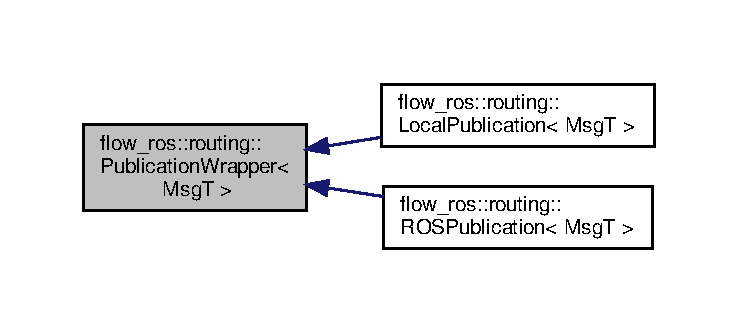
\includegraphics[width=350pt]{classflow__ros_1_1routing_1_1_publication_wrapper__inherit__graph}
\end{center}
\end{figure}
\subsection*{Public Member Functions}
\begin{DoxyCompactItemize}
\item 
virtual void \hyperlink{classflow__ros_1_1routing_1_1_publication_wrapper_a43b9989390bf9f001fe9670a0c1d5897}{publish} (const \hyperlink{namespaceflow__ros_a21a684f38ee2083b3858613317c46d82}{message\+\_\+shared\+\_\+ptr\+\_\+t}$<$ MsgT $>$ \&message) const =0
\begin{DoxyCompactList}\small\item\em Publishes message. \end{DoxyCompactList}\item 
\mbox{\Hypertarget{classflow__ros_1_1routing_1_1_publication_wrapper_a1aa441bb1846211cb803362233d4ee0b}\label{classflow__ros_1_1routing_1_1_publication_wrapper_a1aa441bb1846211cb803362233d4ee0b}} 
virtual std\+::string \hyperlink{classflow__ros_1_1routing_1_1_publication_wrapper_a1aa441bb1846211cb803362233d4ee0b}{get\+Topic} () const =0
\begin{DoxyCompactList}\small\item\em Returns topic associated with publication. \end{DoxyCompactList}\item 
\mbox{\Hypertarget{classflow__ros_1_1routing_1_1_publication_wrapper_a3e2fb2a4cafe729a643af5ed5033dc50}\label{classflow__ros_1_1routing_1_1_publication_wrapper_a3e2fb2a4cafe729a643af5ed5033dc50}} 
virtual std\+::uint32\+\_\+t \hyperlink{classflow__ros_1_1routing_1_1_publication_wrapper_a3e2fb2a4cafe729a643af5ed5033dc50}{get\+Num\+Subscribers} () const =0
\begin{DoxyCompactList}\small\item\em Returns number of subscriptions connected to this publication. \end{DoxyCompactList}\item 
\mbox{\Hypertarget{classflow__ros_1_1routing_1_1_publication_wrapper_a86fdc857e02347e862dbbb113e5a6cb6}\label{classflow__ros_1_1routing_1_1_publication_wrapper_a86fdc857e02347e862dbbb113e5a6cb6}} 
virtual bool \hyperlink{classflow__ros_1_1routing_1_1_publication_wrapper_a86fdc857e02347e862dbbb113e5a6cb6}{is\+Latched} () const =0
\begin{DoxyCompactList}\small\item\em Returns flag indicating whether or not publisher is latched. \end{DoxyCompactList}\item 
\mbox{\Hypertarget{classflow__ros_1_1routing_1_1_publication_wrapper_a0398202c79a6bdb1ff57acc8c730bc65}\label{classflow__ros_1_1routing_1_1_publication_wrapper_a0398202c79a6bdb1ff57acc8c730bc65}} 
virtual \hyperlink{transport__info_8h_ae57afcf849a5bdb82b958347c6ccc57b}{Transport\+Method} \hyperlink{classflow__ros_1_1routing_1_1_publication_wrapper_a0398202c79a6bdb1ff57acc8c730bc65}{get\+Transport\+Method} () const =0
\begin{DoxyCompactList}\small\item\em Returns transport method (code) associated with this publication. \end{DoxyCompactList}\item 
\mbox{\Hypertarget{classflow__ros_1_1routing_1_1_publication_wrapper_afc33bf27092f8e8188e3f7955a6b7c97}\label{classflow__ros_1_1routing_1_1_publication_wrapper_afc33bf27092f8e8188e3f7955a6b7c97}} 
virtual bool \hyperlink{classflow__ros_1_1routing_1_1_publication_wrapper_afc33bf27092f8e8188e3f7955a6b7c97}{is\+Valid} () const =0
\begin{DoxyCompactList}\small\item\em Validity check. \end{DoxyCompactList}\item 
\mbox{\Hypertarget{classflow__ros_1_1routing_1_1_publication_wrapper_ae3d53f17565deb8a0d5b6d971d11e813}\label{classflow__ros_1_1routing_1_1_publication_wrapper_ae3d53f17565deb8a0d5b6d971d11e813}} 
virtual \hyperlink{classflow__ros_1_1routing_1_1_publication_wrapper_ae3d53f17565deb8a0d5b6d971d11e813}{operator bool} () const
\begin{DoxyCompactList}\small\item\em Validity check cast. \end{DoxyCompactList}\end{DoxyCompactItemize}
\subsection*{Static Public Member Functions}
\begin{DoxyCompactItemize}
\item 
\mbox{\Hypertarget{classflow__ros_1_1routing_1_1_publication_wrapper_a5ee03549ef54a9e5cc78d185ad866ec1}\label{classflow__ros_1_1routing_1_1_publication_wrapper_a5ee03549ef54a9e5cc78d185ad866ec1}} 
static constexpr \hyperlink{transport__info_8h_acb4b6ac875de32a0d0ee8cec235f7752}{Direction} \hyperlink{classflow__ros_1_1routing_1_1_publication_wrapper_a5ee03549ef54a9e5cc78d185ad866ec1}{get\+Transport\+Direction} ()
\begin{DoxyCompactList}\small\item\em Returns transport direction (code) associated with this publication. \end{DoxyCompactList}\end{DoxyCompactItemize}


\subsection{Detailed Description}
\subsubsection*{template$<$typename MsgT$>$\newline
class flow\+\_\+ros\+::routing\+::\+Publication\+Wrapper$<$ Msg\+T $>$}

C\+R\+T\+P-\/base for message publishing objects. 

\subsection{Member Function Documentation}
\mbox{\Hypertarget{classflow__ros_1_1routing_1_1_publication_wrapper_a43b9989390bf9f001fe9670a0c1d5897}\label{classflow__ros_1_1routing_1_1_publication_wrapper_a43b9989390bf9f001fe9670a0c1d5897}} 
\index{flow\+\_\+ros\+::routing\+::\+Publication\+Wrapper@{flow\+\_\+ros\+::routing\+::\+Publication\+Wrapper}!publish@{publish}}
\index{publish@{publish}!flow\+\_\+ros\+::routing\+::\+Publication\+Wrapper@{flow\+\_\+ros\+::routing\+::\+Publication\+Wrapper}}
\subsubsection{\texorpdfstring{publish()}{publish()}}
{\footnotesize\ttfamily template$<$typename MsgT $>$ \\
virtual void \hyperlink{classflow__ros_1_1routing_1_1_publication_wrapper}{flow\+\_\+ros\+::routing\+::\+Publication\+Wrapper}$<$ MsgT $>$\+::publish (\begin{DoxyParamCaption}\item[{const \hyperlink{namespaceflow__ros_a21a684f38ee2083b3858613317c46d82}{message\+\_\+shared\+\_\+ptr\+\_\+t}$<$ MsgT $>$ \&}]{message }\end{DoxyParamCaption}) const\hspace{0.3cm}{\ttfamily [pure virtual]}}



Publishes message. 


\begin{DoxyParams}{Parameters}
{\em message} & message data to publish \\
\hline
\end{DoxyParams}


Implemented in \hyperlink{classflow__ros_1_1routing_1_1_local_publication_ab2d53a2bd93e83ee11095f35d5820226}{flow\+\_\+ros\+::routing\+::\+Local\+Publication$<$ Msg\+T $>$}, and \hyperlink{classflow__ros_1_1routing_1_1_r_o_s_publication_a1ad3cf68c465a909399bb4496e561f0b}{flow\+\_\+ros\+::routing\+::\+R\+O\+S\+Publication$<$ Msg\+T $>$}.



The documentation for this class was generated from the following file\+:\begin{DoxyCompactItemize}
\item 
flow\+\_\+ros/include/routing/publication\+\_\+wrapper.\+h\end{DoxyCompactItemize}

\hypertarget{classflow__ros_1_1_publisher}{}\section{flow\+\_\+ros\+:\+:Publisher$<$ MsgT $>$ Class Template Reference}
\label{classflow__ros_1_1_publisher}\index{flow\+\_\+ros\+::\+Publisher$<$ Msg\+T $>$@{flow\+\_\+ros\+::\+Publisher$<$ Msg\+T $>$}}


Output channel which publishes messages.  




{\ttfamily \#include $<$publisher.\+h$>$}



Inheritance diagram for flow\+\_\+ros\+:\+:Publisher$<$ MsgT $>$\+:\nopagebreak
\begin{figure}[H]
\begin{center}
\leavevmode
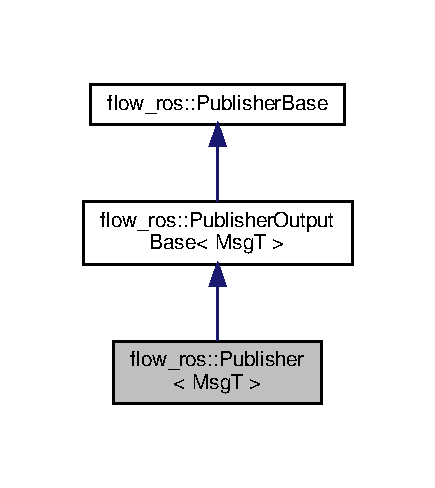
\includegraphics[width=209pt]{classflow__ros_1_1_publisher__inherit__graph}
\end{center}
\end{figure}


Collaboration diagram for flow\+\_\+ros\+:\+:Publisher$<$ MsgT $>$\+:\nopagebreak
\begin{figure}[H]
\begin{center}
\leavevmode
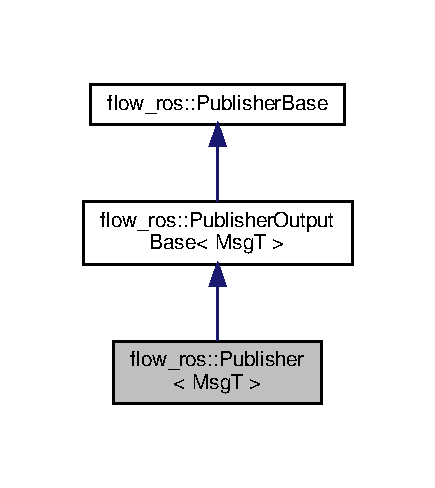
\includegraphics[width=209pt]{classflow__ros_1_1_publisher__coll__graph}
\end{center}
\end{figure}
\subsection*{Public Member Functions}
\begin{DoxyCompactItemize}
\item 
\hyperlink{classflow__ros_1_1_publisher_a51a76fa72d57c38e23857c0c95103ef4}{Publisher} (ros\+::\+Node\+Handle \&nh, const std\+::string \&topic, std\+::uint32\+\_\+t queue\+\_\+size=0, const bool latched=false)
\begin{DoxyCompactList}\small\item\em {\ttfamily ros\+::\+Node\+Handle} setup constructor (extra-\/node messaging) \end{DoxyCompactList}\item 
\hyperlink{classflow__ros_1_1_publisher_a2a5c14b45b30efa5227c6b5b2586ab7e}{Publisher} (\hyperlink{classflow__ros_1_1_router}{Router} \&pb, std\+::string topic, std\+::uint32\+\_\+t queue\+\_\+size=0, const bool latched=false)
\begin{DoxyCompactList}\small\item\em {\ttfamily \hyperlink{classflow__ros_1_1_router}{Router}} setup constructor (intra-\/node messaging) \end{DoxyCompactList}\item 
void \hyperlink{classflow__ros_1_1_publisher_abba3d43e5dfe0bc1690fd4980e2f927f}{publish} (\hyperlink{namespaceflow__ros_a21a684f38ee2083b3858613317c46d82}{message\+\_\+shared\+\_\+ptr\+\_\+t}$<$ MsgT $>$ msg) const
\begin{DoxyCompactList}\small\item\em Publishes output message. \end{DoxyCompactList}\end{DoxyCompactItemize}
\subsection*{Additional Inherited Members}


\subsection{Detailed Description}
\subsubsection*{template$<$typename MsgT$>$\newline
class flow\+\_\+ros\+::\+Publisher$<$ Msg\+T $>$}

Output channel which publishes messages. 


\begin{DoxyTemplParams}{Template Parameters}
{\em MsgT} & message type \\
\hline
\end{DoxyTemplParams}


\subsection{Constructor \& Destructor Documentation}
\mbox{\Hypertarget{classflow__ros_1_1_publisher_a51a76fa72d57c38e23857c0c95103ef4}\label{classflow__ros_1_1_publisher_a51a76fa72d57c38e23857c0c95103ef4}} 
\index{flow\+\_\+ros\+::\+Publisher@{flow\+\_\+ros\+::\+Publisher}!Publisher@{Publisher}}
\index{Publisher@{Publisher}!flow\+\_\+ros\+::\+Publisher@{flow\+\_\+ros\+::\+Publisher}}
\subsubsection{\texorpdfstring{Publisher()}{Publisher()}\hspace{0.1cm}{\footnotesize\ttfamily [1/2]}}
{\footnotesize\ttfamily template$<$typename MsgT$>$ \\
\hyperlink{classflow__ros_1_1_publisher}{flow\+\_\+ros\+::\+Publisher}$<$ MsgT $>$\+::\hyperlink{classflow__ros_1_1_publisher}{Publisher} (\begin{DoxyParamCaption}\item[{ros\+::\+Node\+Handle \&}]{nh,  }\item[{const std\+::string \&}]{topic,  }\item[{std\+::uint32\+\_\+t}]{queue\+\_\+size = {\ttfamily 0},  }\item[{const bool}]{latched = {\ttfamily false} }\end{DoxyParamCaption})\hspace{0.3cm}{\ttfamily [inline]}}



{\ttfamily ros\+::\+Node\+Handle} setup constructor (extra-\/node messaging) 


\begin{DoxyParams}[1]{Parameters}
\mbox{\tt in,out}  & {\em nh} & R\+OS node handle to negotiate topic advertisement/connection \\
\hline
 & {\em topic} & topic associated with messages to be output \\
\hline
 & {\em queue\+\_\+size} & underlying R\+OS publisher queue size \\
\hline
 & {\em latched} & options for creating a \char`\"{}latched\char`\"{} output publisher\\
\hline
\end{DoxyParams}
\begin{DoxyWarning}{Warning}
Will throw with {\ttfamily std\+::runtime\+\_\+error} if underlying publisher could not be establish a connection with R\+O\+S-\/master 
\end{DoxyWarning}
\mbox{\Hypertarget{classflow__ros_1_1_publisher_a2a5c14b45b30efa5227c6b5b2586ab7e}\label{classflow__ros_1_1_publisher_a2a5c14b45b30efa5227c6b5b2586ab7e}} 
\index{flow\+\_\+ros\+::\+Publisher@{flow\+\_\+ros\+::\+Publisher}!Publisher@{Publisher}}
\index{Publisher@{Publisher}!flow\+\_\+ros\+::\+Publisher@{flow\+\_\+ros\+::\+Publisher}}
\subsubsection{\texorpdfstring{Publisher()}{Publisher()}\hspace{0.1cm}{\footnotesize\ttfamily [2/2]}}
{\footnotesize\ttfamily template$<$typename MsgT$>$ \\
\hyperlink{classflow__ros_1_1_publisher}{flow\+\_\+ros\+::\+Publisher}$<$ MsgT $>$\+::\hyperlink{classflow__ros_1_1_publisher}{Publisher} (\begin{DoxyParamCaption}\item[{\hyperlink{classflow__ros_1_1_router}{Router} \&}]{pb,  }\item[{std\+::string}]{topic,  }\item[{std\+::uint32\+\_\+t}]{queue\+\_\+size = {\ttfamily 0},  }\item[{const bool}]{latched = {\ttfamily false} }\end{DoxyParamCaption})\hspace{0.3cm}{\ttfamily [inline]}}



{\ttfamily \hyperlink{classflow__ros_1_1_router}{Router}} setup constructor (intra-\/node messaging) 


\begin{DoxyParams}[1]{Parameters}
\mbox{\tt in,out}  & {\em pb} & Intra-\/node \hyperlink{classflow__ros_1_1_router}{Router} routing object \\
\hline
 & {\em topic} & topic associated with messages to be output \\
\hline
 & {\em queue\+\_\+size} & underlying publication queue size \\
\hline
 & {\em latched} & not used; dummy for A\+PI consistency\\
\hline
\end{DoxyParams}
\begin{DoxyWarning}{Warning}
Will throw with {\ttfamily std\+::runtime\+\_\+error} if underlying publisher could not be establish a connection with R\+O\+S-\/master 
\end{DoxyWarning}


\subsection{Member Function Documentation}
\mbox{\Hypertarget{classflow__ros_1_1_publisher_abba3d43e5dfe0bc1690fd4980e2f927f}\label{classflow__ros_1_1_publisher_abba3d43e5dfe0bc1690fd4980e2f927f}} 
\index{flow\+\_\+ros\+::\+Publisher@{flow\+\_\+ros\+::\+Publisher}!publish@{publish}}
\index{publish@{publish}!flow\+\_\+ros\+::\+Publisher@{flow\+\_\+ros\+::\+Publisher}}
\subsubsection{\texorpdfstring{publish()}{publish()}}
{\footnotesize\ttfamily template$<$typename MsgT$>$ \\
void \hyperlink{classflow__ros_1_1_publisher}{flow\+\_\+ros\+::\+Publisher}$<$ MsgT $>$\+::publish (\begin{DoxyParamCaption}\item[{\hyperlink{namespaceflow__ros_a21a684f38ee2083b3858613317c46d82}{message\+\_\+shared\+\_\+ptr\+\_\+t}$<$ MsgT $>$}]{msg }\end{DoxyParamCaption}) const\hspace{0.3cm}{\ttfamily [inline]}}



Publishes output message. 

If message resource is invalid (i.\+e. {\ttfamily msg == nullptr}), then no message is sent over underlying publication channel


\begin{DoxyParams}{Parameters}
{\em msg} & next output message \\
\hline
\end{DoxyParams}


The documentation for this class was generated from the following file\+:\begin{DoxyCompactItemize}
\item 
flow\+\_\+ros/include/\hyperlink{publisher_8h}{publisher.\+h}\end{DoxyCompactItemize}

\hypertarget{classflow__ros_1_1_publisher_base}{}\section{flow\+\_\+ros\+:\+:Publisher\+Base Class Reference}
\label{classflow__ros_1_1_publisher_base}\index{flow\+\_\+ros\+::\+Publisher\+Base@{flow\+\_\+ros\+::\+Publisher\+Base}}


Publish base to expose meta-\/information methods.  




{\ttfamily \#include $<$publisher.\+h$>$}



Inheritance diagram for flow\+\_\+ros\+:\+:Publisher\+Base\+:\nopagebreak
\begin{figure}[H]
\begin{center}
\leavevmode
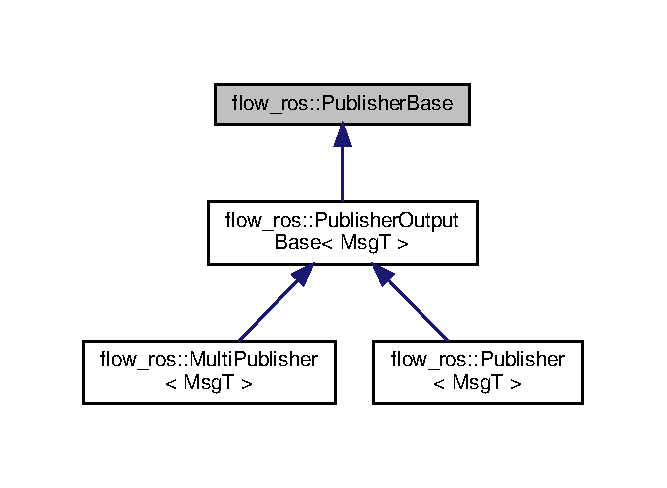
\includegraphics[width=320pt]{classflow__ros_1_1_publisher_base__inherit__graph}
\end{center}
\end{figure}
\subsection*{Public Member Functions}
\begin{DoxyCompactItemize}
\item 
virtual std\+::string \hyperlink{classflow__ros_1_1_publisher_base_aed36dfd3c58ff3c588b2030319cd26e1}{get\+Topic} () const =0
\begin{DoxyCompactList}\small\item\em Returns topic associated with publication. \end{DoxyCompactList}\item 
virtual std\+::uint32\+\_\+t \hyperlink{classflow__ros_1_1_publisher_base_ae5638184ee60bbc1326a5e7b47919bec}{get\+Num\+Subscribers} () const =0
\begin{DoxyCompactList}\small\item\em Returns number of subscriptions connected to this publication. \end{DoxyCompactList}\item 
virtual bool \hyperlink{classflow__ros_1_1_publisher_base_a51ef6d34734d3dc39053234491665d2c}{is\+Latched} () const =0
\begin{DoxyCompactList}\small\item\em Returns flag indicating whether or not publisher is latched. \end{DoxyCompactList}\item 
virtual \hyperlink{transport__info_8h_ae57afcf849a5bdb82b958347c6ccc57b}{routing\+::\+Transport\+Method} \hyperlink{classflow__ros_1_1_publisher_base_ad0cd41b4d2a8e4697610643c7e90d8c7}{get\+Transport\+Method} () const =0
\begin{DoxyCompactList}\small\item\em Returns transport method (code) associated with this publication. \end{DoxyCompactList}\item 
virtual bool \hyperlink{classflow__ros_1_1_publisher_base_ac9bc27703de2394a0e1f3df7dac93548}{is\+Valid} () const =0
\begin{DoxyCompactList}\small\item\em Validity check. \end{DoxyCompactList}\end{DoxyCompactItemize}


\subsection{Detailed Description}
Publish base to expose meta-\/information methods. 

\subsection{Member Function Documentation}
\mbox{\Hypertarget{classflow__ros_1_1_publisher_base_ae5638184ee60bbc1326a5e7b47919bec}\label{classflow__ros_1_1_publisher_base_ae5638184ee60bbc1326a5e7b47919bec}} 
\index{flow\+\_\+ros\+::\+Publisher\+Base@{flow\+\_\+ros\+::\+Publisher\+Base}!get\+Num\+Subscribers@{get\+Num\+Subscribers}}
\index{get\+Num\+Subscribers@{get\+Num\+Subscribers}!flow\+\_\+ros\+::\+Publisher\+Base@{flow\+\_\+ros\+::\+Publisher\+Base}}
\subsubsection{\texorpdfstring{get\+Num\+Subscribers()}{getNumSubscribers()}}
{\footnotesize\ttfamily virtual std\+::uint32\+\_\+t flow\+\_\+ros\+::\+Publisher\+Base\+::get\+Num\+Subscribers (\begin{DoxyParamCaption}{ }\end{DoxyParamCaption}) const\hspace{0.3cm}{\ttfamily [pure virtual]}}



Returns number of subscriptions connected to this publication. 



Implemented in \hyperlink{classflow__ros_1_1_publisher_output_base_a8f51f3d329d65aad7d0f9ea6b4f3c4b6}{flow\+\_\+ros\+::\+Publisher\+Output\+Base$<$ Msg\+T $>$}.

\mbox{\Hypertarget{classflow__ros_1_1_publisher_base_aed36dfd3c58ff3c588b2030319cd26e1}\label{classflow__ros_1_1_publisher_base_aed36dfd3c58ff3c588b2030319cd26e1}} 
\index{flow\+\_\+ros\+::\+Publisher\+Base@{flow\+\_\+ros\+::\+Publisher\+Base}!get\+Topic@{get\+Topic}}
\index{get\+Topic@{get\+Topic}!flow\+\_\+ros\+::\+Publisher\+Base@{flow\+\_\+ros\+::\+Publisher\+Base}}
\subsubsection{\texorpdfstring{get\+Topic()}{getTopic()}}
{\footnotesize\ttfamily virtual std\+::string flow\+\_\+ros\+::\+Publisher\+Base\+::get\+Topic (\begin{DoxyParamCaption}{ }\end{DoxyParamCaption}) const\hspace{0.3cm}{\ttfamily [pure virtual]}}



Returns topic associated with publication. 



Implemented in \hyperlink{classflow__ros_1_1_publisher_output_base_a28d4636b7d52e0dac54f27556308e9d4}{flow\+\_\+ros\+::\+Publisher\+Output\+Base$<$ Msg\+T $>$}.

\mbox{\Hypertarget{classflow__ros_1_1_publisher_base_ad0cd41b4d2a8e4697610643c7e90d8c7}\label{classflow__ros_1_1_publisher_base_ad0cd41b4d2a8e4697610643c7e90d8c7}} 
\index{flow\+\_\+ros\+::\+Publisher\+Base@{flow\+\_\+ros\+::\+Publisher\+Base}!get\+Transport\+Method@{get\+Transport\+Method}}
\index{get\+Transport\+Method@{get\+Transport\+Method}!flow\+\_\+ros\+::\+Publisher\+Base@{flow\+\_\+ros\+::\+Publisher\+Base}}
\subsubsection{\texorpdfstring{get\+Transport\+Method()}{getTransportMethod()}}
{\footnotesize\ttfamily virtual \hyperlink{transport__info_8h_ae57afcf849a5bdb82b958347c6ccc57b}{routing\+::\+Transport\+Method} flow\+\_\+ros\+::\+Publisher\+Base\+::get\+Transport\+Method (\begin{DoxyParamCaption}{ }\end{DoxyParamCaption}) const\hspace{0.3cm}{\ttfamily [pure virtual]}}



Returns transport method (code) associated with this publication. 



Implemented in \hyperlink{classflow__ros_1_1_publisher_output_base_ac052232bb5a6fb9ea04ab61453d14f69}{flow\+\_\+ros\+::\+Publisher\+Output\+Base$<$ Msg\+T $>$}.

\mbox{\Hypertarget{classflow__ros_1_1_publisher_base_a51ef6d34734d3dc39053234491665d2c}\label{classflow__ros_1_1_publisher_base_a51ef6d34734d3dc39053234491665d2c}} 
\index{flow\+\_\+ros\+::\+Publisher\+Base@{flow\+\_\+ros\+::\+Publisher\+Base}!is\+Latched@{is\+Latched}}
\index{is\+Latched@{is\+Latched}!flow\+\_\+ros\+::\+Publisher\+Base@{flow\+\_\+ros\+::\+Publisher\+Base}}
\subsubsection{\texorpdfstring{is\+Latched()}{isLatched()}}
{\footnotesize\ttfamily virtual bool flow\+\_\+ros\+::\+Publisher\+Base\+::is\+Latched (\begin{DoxyParamCaption}{ }\end{DoxyParamCaption}) const\hspace{0.3cm}{\ttfamily [pure virtual]}}



Returns flag indicating whether or not publisher is latched. 



Implemented in \hyperlink{classflow__ros_1_1_publisher_output_base_a34acf851a9aa31ece46b6b5887b3db24}{flow\+\_\+ros\+::\+Publisher\+Output\+Base$<$ Msg\+T $>$}.

\mbox{\Hypertarget{classflow__ros_1_1_publisher_base_ac9bc27703de2394a0e1f3df7dac93548}\label{classflow__ros_1_1_publisher_base_ac9bc27703de2394a0e1f3df7dac93548}} 
\index{flow\+\_\+ros\+::\+Publisher\+Base@{flow\+\_\+ros\+::\+Publisher\+Base}!is\+Valid@{is\+Valid}}
\index{is\+Valid@{is\+Valid}!flow\+\_\+ros\+::\+Publisher\+Base@{flow\+\_\+ros\+::\+Publisher\+Base}}
\subsubsection{\texorpdfstring{is\+Valid()}{isValid()}}
{\footnotesize\ttfamily virtual bool flow\+\_\+ros\+::\+Publisher\+Base\+::is\+Valid (\begin{DoxyParamCaption}{ }\end{DoxyParamCaption}) const\hspace{0.3cm}{\ttfamily [pure virtual]}}



Validity check. 



Implemented in \hyperlink{classflow__ros_1_1_publisher_output_base_a60ffa435ac1243b046d8029584c097a3}{flow\+\_\+ros\+::\+Publisher\+Output\+Base$<$ Msg\+T $>$}.



The documentation for this class was generated from the following file\+:\begin{DoxyCompactItemize}
\item 
flow\+\_\+ros/include/\hyperlink{publisher_8h}{publisher.\+h}\end{DoxyCompactItemize}

\hypertarget{classflow__ros_1_1_publisher_output_base}{}\section{flow\+\_\+ros\+:\+:Publisher\+Output\+Base$<$ MsgT $>$ Class Template Reference}
\label{classflow__ros_1_1_publisher_output_base}\index{flow\+\_\+ros\+::\+Publisher\+Output\+Base$<$ Msg\+T $>$@{flow\+\_\+ros\+::\+Publisher\+Output\+Base$<$ Msg\+T $>$}}


Message publisher base type.  




{\ttfamily \#include $<$publisher.\+h$>$}



Inheritance diagram for flow\+\_\+ros\+:\+:Publisher\+Output\+Base$<$ MsgT $>$\+:\nopagebreak
\begin{figure}[H]
\begin{center}
\leavevmode
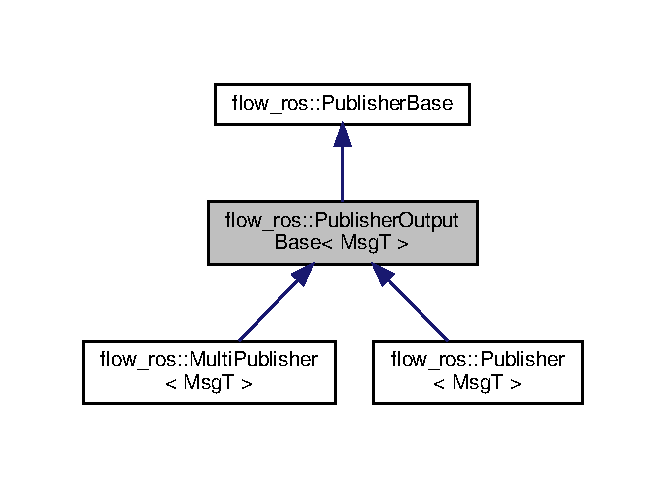
\includegraphics[width=320pt]{classflow__ros_1_1_publisher_output_base__inherit__graph}
\end{center}
\end{figure}


Collaboration diagram for flow\+\_\+ros\+:\+:Publisher\+Output\+Base$<$ MsgT $>$\+:\nopagebreak
\begin{figure}[H]
\begin{center}
\leavevmode
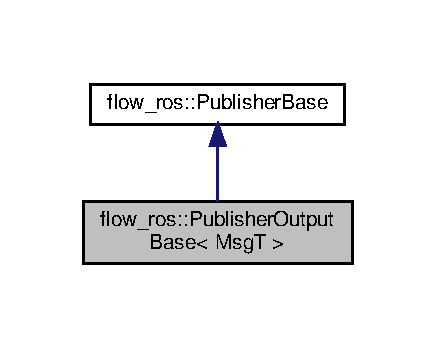
\includegraphics[width=209pt]{classflow__ros_1_1_publisher_output_base__coll__graph}
\end{center}
\end{figure}
\subsection*{Public Member Functions}
\begin{DoxyCompactItemize}
\item 
std\+::string \hyperlink{classflow__ros_1_1_publisher_output_base_a28d4636b7d52e0dac54f27556308e9d4}{get\+Topic} () const final
\begin{DoxyCompactList}\small\item\em Returns topic associated with publication. \end{DoxyCompactList}\item 
std\+::uint32\+\_\+t \hyperlink{classflow__ros_1_1_publisher_output_base_a8f51f3d329d65aad7d0f9ea6b4f3c4b6}{get\+Num\+Subscribers} () const final
\begin{DoxyCompactList}\small\item\em Returns number of subscriptions connected to this publication. \end{DoxyCompactList}\item 
bool \hyperlink{classflow__ros_1_1_publisher_output_base_a34acf851a9aa31ece46b6b5887b3db24}{is\+Latched} () const final
\begin{DoxyCompactList}\small\item\em Returns flag indicating whether or not publisher is latched. \end{DoxyCompactList}\item 
\hyperlink{transport__info_8h_ae57afcf849a5bdb82b958347c6ccc57b}{routing\+::\+Transport\+Method} \hyperlink{classflow__ros_1_1_publisher_output_base_ac052232bb5a6fb9ea04ab61453d14f69}{get\+Transport\+Method} () const final
\begin{DoxyCompactList}\small\item\em Returns transport method (code) associated with this publication. \end{DoxyCompactList}\item 
bool \hyperlink{classflow__ros_1_1_publisher_output_base_a60ffa435ac1243b046d8029584c097a3}{is\+Valid} () const final
\begin{DoxyCompactList}\small\item\em Validity check. \end{DoxyCompactList}\end{DoxyCompactItemize}
\subsection*{Static Public Member Functions}
\begin{DoxyCompactItemize}
\item 
static constexpr \hyperlink{transport__info_8h_acb4b6ac875de32a0d0ee8cec235f7752}{routing\+::\+Direction} \hyperlink{classflow__ros_1_1_publisher_output_base_a4f42e2bf09aa92117879071652a0df17}{get\+Transport\+Direction} ()
\begin{DoxyCompactList}\small\item\em Returns transport direction (code) associated with this publication. \end{DoxyCompactList}\end{DoxyCompactItemize}
\subsection*{Protected Member Functions}
\begin{DoxyCompactItemize}
\item 
\hyperlink{classflow__ros_1_1_publisher_output_base_a9e937b3b34f0a78ea03826b484dfa354}{Publisher\+Output\+Base} (std\+::shared\+\_\+ptr$<$ \hyperlink{classflow__ros_1_1routing_1_1_publication_wrapper}{routing\+::\+Publication\+Wrapper}$<$ MsgT $>$$>$ pub)
\begin{DoxyCompactList}\small\item\em Publication setup constructor (generic) \end{DoxyCompactList}\item 
void \hyperlink{classflow__ros_1_1_publisher_output_base_a66abc7f5296a4b2c29c776539df70cd1}{publish} (const \hyperlink{namespaceflow__ros_a21a684f38ee2083b3858613317c46d82}{message\+\_\+shared\+\_\+ptr\+\_\+t}$<$ MsgT $>$ \&message) const
\begin{DoxyCompactList}\small\item\em Call all held subscriber callbacks on message being published. \end{DoxyCompactList}\end{DoxyCompactItemize}


\subsection{Detailed Description}
\subsubsection*{template$<$typename MsgT$>$\newline
class flow\+\_\+ros\+::\+Publisher\+Output\+Base$<$ Msg\+T $>$}

Message publisher base type. 


\begin{DoxyTemplParams}{Template Parameters}
{\em MsgT} & Message type \\
\hline
\end{DoxyTemplParams}


\subsection{Constructor \& Destructor Documentation}
\mbox{\Hypertarget{classflow__ros_1_1_publisher_output_base_a9e937b3b34f0a78ea03826b484dfa354}\label{classflow__ros_1_1_publisher_output_base_a9e937b3b34f0a78ea03826b484dfa354}} 
\index{flow\+\_\+ros\+::\+Publisher\+Output\+Base@{flow\+\_\+ros\+::\+Publisher\+Output\+Base}!Publisher\+Output\+Base@{Publisher\+Output\+Base}}
\index{Publisher\+Output\+Base@{Publisher\+Output\+Base}!flow\+\_\+ros\+::\+Publisher\+Output\+Base@{flow\+\_\+ros\+::\+Publisher\+Output\+Base}}
\subsubsection{\texorpdfstring{Publisher\+Output\+Base()}{PublisherOutputBase()}}
{\footnotesize\ttfamily template$<$typename MsgT $>$ \\
\hyperlink{classflow__ros_1_1_publisher_output_base}{flow\+\_\+ros\+::\+Publisher\+Output\+Base}$<$ MsgT $>$\+::\hyperlink{classflow__ros_1_1_publisher_output_base}{Publisher\+Output\+Base} (\begin{DoxyParamCaption}\item[{std\+::shared\+\_\+ptr$<$ \hyperlink{classflow__ros_1_1routing_1_1_publication_wrapper}{routing\+::\+Publication\+Wrapper}$<$ MsgT $>$$>$}]{pub }\end{DoxyParamCaption})\hspace{0.3cm}{\ttfamily [inline]}, {\ttfamily [explicit]}, {\ttfamily [protected]}}



Publication setup constructor (generic) 


\begin{DoxyParams}{Parameters}
{\em pub} & publication resource \\
\hline
\end{DoxyParams}


\subsection{Member Function Documentation}
\mbox{\Hypertarget{classflow__ros_1_1_publisher_output_base_a8f51f3d329d65aad7d0f9ea6b4f3c4b6}\label{classflow__ros_1_1_publisher_output_base_a8f51f3d329d65aad7d0f9ea6b4f3c4b6}} 
\index{flow\+\_\+ros\+::\+Publisher\+Output\+Base@{flow\+\_\+ros\+::\+Publisher\+Output\+Base}!get\+Num\+Subscribers@{get\+Num\+Subscribers}}
\index{get\+Num\+Subscribers@{get\+Num\+Subscribers}!flow\+\_\+ros\+::\+Publisher\+Output\+Base@{flow\+\_\+ros\+::\+Publisher\+Output\+Base}}
\subsubsection{\texorpdfstring{get\+Num\+Subscribers()}{getNumSubscribers()}}
{\footnotesize\ttfamily template$<$typename MsgT $>$ \\
std\+::uint32\+\_\+t \hyperlink{classflow__ros_1_1_publisher_output_base}{flow\+\_\+ros\+::\+Publisher\+Output\+Base}$<$ MsgT $>$\+::get\+Num\+Subscribers (\begin{DoxyParamCaption}{ }\end{DoxyParamCaption}) const\hspace{0.3cm}{\ttfamily [inline]}, {\ttfamily [final]}, {\ttfamily [virtual]}}



Returns number of subscriptions connected to this publication. 



Implements \hyperlink{classflow__ros_1_1_publisher_base_ae5638184ee60bbc1326a5e7b47919bec}{flow\+\_\+ros\+::\+Publisher\+Base}.

\mbox{\Hypertarget{classflow__ros_1_1_publisher_output_base_a28d4636b7d52e0dac54f27556308e9d4}\label{classflow__ros_1_1_publisher_output_base_a28d4636b7d52e0dac54f27556308e9d4}} 
\index{flow\+\_\+ros\+::\+Publisher\+Output\+Base@{flow\+\_\+ros\+::\+Publisher\+Output\+Base}!get\+Topic@{get\+Topic}}
\index{get\+Topic@{get\+Topic}!flow\+\_\+ros\+::\+Publisher\+Output\+Base@{flow\+\_\+ros\+::\+Publisher\+Output\+Base}}
\subsubsection{\texorpdfstring{get\+Topic()}{getTopic()}}
{\footnotesize\ttfamily template$<$typename MsgT $>$ \\
std\+::string \hyperlink{classflow__ros_1_1_publisher_output_base}{flow\+\_\+ros\+::\+Publisher\+Output\+Base}$<$ MsgT $>$\+::get\+Topic (\begin{DoxyParamCaption}{ }\end{DoxyParamCaption}) const\hspace{0.3cm}{\ttfamily [inline]}, {\ttfamily [final]}, {\ttfamily [virtual]}}



Returns topic associated with publication. 



Implements \hyperlink{classflow__ros_1_1_publisher_base_aed36dfd3c58ff3c588b2030319cd26e1}{flow\+\_\+ros\+::\+Publisher\+Base}.

\mbox{\Hypertarget{classflow__ros_1_1_publisher_output_base_a4f42e2bf09aa92117879071652a0df17}\label{classflow__ros_1_1_publisher_output_base_a4f42e2bf09aa92117879071652a0df17}} 
\index{flow\+\_\+ros\+::\+Publisher\+Output\+Base@{flow\+\_\+ros\+::\+Publisher\+Output\+Base}!get\+Transport\+Direction@{get\+Transport\+Direction}}
\index{get\+Transport\+Direction@{get\+Transport\+Direction}!flow\+\_\+ros\+::\+Publisher\+Output\+Base@{flow\+\_\+ros\+::\+Publisher\+Output\+Base}}
\subsubsection{\texorpdfstring{get\+Transport\+Direction()}{getTransportDirection()}}
{\footnotesize\ttfamily template$<$typename MsgT $>$ \\
static constexpr \hyperlink{transport__info_8h_acb4b6ac875de32a0d0ee8cec235f7752}{routing\+::\+Direction} \hyperlink{classflow__ros_1_1_publisher_output_base}{flow\+\_\+ros\+::\+Publisher\+Output\+Base}$<$ MsgT $>$\+::get\+Transport\+Direction (\begin{DoxyParamCaption}{ }\end{DoxyParamCaption})\hspace{0.3cm}{\ttfamily [inline]}, {\ttfamily [static]}}



Returns transport direction (code) associated with this publication. 

\mbox{\Hypertarget{classflow__ros_1_1_publisher_output_base_ac052232bb5a6fb9ea04ab61453d14f69}\label{classflow__ros_1_1_publisher_output_base_ac052232bb5a6fb9ea04ab61453d14f69}} 
\index{flow\+\_\+ros\+::\+Publisher\+Output\+Base@{flow\+\_\+ros\+::\+Publisher\+Output\+Base}!get\+Transport\+Method@{get\+Transport\+Method}}
\index{get\+Transport\+Method@{get\+Transport\+Method}!flow\+\_\+ros\+::\+Publisher\+Output\+Base@{flow\+\_\+ros\+::\+Publisher\+Output\+Base}}
\subsubsection{\texorpdfstring{get\+Transport\+Method()}{getTransportMethod()}}
{\footnotesize\ttfamily template$<$typename MsgT $>$ \\
\hyperlink{transport__info_8h_ae57afcf849a5bdb82b958347c6ccc57b}{routing\+::\+Transport\+Method} \hyperlink{classflow__ros_1_1_publisher_output_base}{flow\+\_\+ros\+::\+Publisher\+Output\+Base}$<$ MsgT $>$\+::get\+Transport\+Method (\begin{DoxyParamCaption}{ }\end{DoxyParamCaption}) const\hspace{0.3cm}{\ttfamily [inline]}, {\ttfamily [final]}, {\ttfamily [virtual]}}



Returns transport method (code) associated with this publication. 



Implements \hyperlink{classflow__ros_1_1_publisher_base_ad0cd41b4d2a8e4697610643c7e90d8c7}{flow\+\_\+ros\+::\+Publisher\+Base}.

\mbox{\Hypertarget{classflow__ros_1_1_publisher_output_base_a34acf851a9aa31ece46b6b5887b3db24}\label{classflow__ros_1_1_publisher_output_base_a34acf851a9aa31ece46b6b5887b3db24}} 
\index{flow\+\_\+ros\+::\+Publisher\+Output\+Base@{flow\+\_\+ros\+::\+Publisher\+Output\+Base}!is\+Latched@{is\+Latched}}
\index{is\+Latched@{is\+Latched}!flow\+\_\+ros\+::\+Publisher\+Output\+Base@{flow\+\_\+ros\+::\+Publisher\+Output\+Base}}
\subsubsection{\texorpdfstring{is\+Latched()}{isLatched()}}
{\footnotesize\ttfamily template$<$typename MsgT $>$ \\
bool \hyperlink{classflow__ros_1_1_publisher_output_base}{flow\+\_\+ros\+::\+Publisher\+Output\+Base}$<$ MsgT $>$\+::is\+Latched (\begin{DoxyParamCaption}{ }\end{DoxyParamCaption}) const\hspace{0.3cm}{\ttfamily [inline]}, {\ttfamily [final]}, {\ttfamily [virtual]}}



Returns flag indicating whether or not publisher is latched. 



Implements \hyperlink{classflow__ros_1_1_publisher_base_a51ef6d34734d3dc39053234491665d2c}{flow\+\_\+ros\+::\+Publisher\+Base}.

\mbox{\Hypertarget{classflow__ros_1_1_publisher_output_base_a60ffa435ac1243b046d8029584c097a3}\label{classflow__ros_1_1_publisher_output_base_a60ffa435ac1243b046d8029584c097a3}} 
\index{flow\+\_\+ros\+::\+Publisher\+Output\+Base@{flow\+\_\+ros\+::\+Publisher\+Output\+Base}!is\+Valid@{is\+Valid}}
\index{is\+Valid@{is\+Valid}!flow\+\_\+ros\+::\+Publisher\+Output\+Base@{flow\+\_\+ros\+::\+Publisher\+Output\+Base}}
\subsubsection{\texorpdfstring{is\+Valid()}{isValid()}}
{\footnotesize\ttfamily template$<$typename MsgT $>$ \\
bool \hyperlink{classflow__ros_1_1_publisher_output_base}{flow\+\_\+ros\+::\+Publisher\+Output\+Base}$<$ MsgT $>$\+::is\+Valid (\begin{DoxyParamCaption}{ }\end{DoxyParamCaption}) const\hspace{0.3cm}{\ttfamily [inline]}, {\ttfamily [final]}, {\ttfamily [virtual]}}



Validity check. 



Implements \hyperlink{classflow__ros_1_1_publisher_base_ac9bc27703de2394a0e1f3df7dac93548}{flow\+\_\+ros\+::\+Publisher\+Base}.

\mbox{\Hypertarget{classflow__ros_1_1_publisher_output_base_a66abc7f5296a4b2c29c776539df70cd1}\label{classflow__ros_1_1_publisher_output_base_a66abc7f5296a4b2c29c776539df70cd1}} 
\index{flow\+\_\+ros\+::\+Publisher\+Output\+Base@{flow\+\_\+ros\+::\+Publisher\+Output\+Base}!publish@{publish}}
\index{publish@{publish}!flow\+\_\+ros\+::\+Publisher\+Output\+Base@{flow\+\_\+ros\+::\+Publisher\+Output\+Base}}
\subsubsection{\texorpdfstring{publish()}{publish()}}
{\footnotesize\ttfamily template$<$typename MsgT $>$ \\
void \hyperlink{classflow__ros_1_1_publisher_output_base}{flow\+\_\+ros\+::\+Publisher\+Output\+Base}$<$ MsgT $>$\+::publish (\begin{DoxyParamCaption}\item[{const \hyperlink{namespaceflow__ros_a21a684f38ee2083b3858613317c46d82}{message\+\_\+shared\+\_\+ptr\+\_\+t}$<$ MsgT $>$ \&}]{message }\end{DoxyParamCaption}) const\hspace{0.3cm}{\ttfamily [inline]}, {\ttfamily [protected]}}



Call all held subscriber callbacks on message being published. 


\begin{DoxyParams}{Parameters}
{\em message} & message data to publish \\
\hline
\end{DoxyParams}


The documentation for this class was generated from the following file\+:\begin{DoxyCompactItemize}
\item 
flow\+\_\+ros/include/\hyperlink{publisher_8h}{publisher.\+h}\end{DoxyCompactItemize}

\hypertarget{structflow__ros_1_1_publisher_traits}{}\section{flow\+\_\+ros\+:\+:Publisher\+Traits$<$ MsgT $>$ Struct Template Reference}
\label{structflow__ros_1_1_publisher_traits}\index{flow\+\_\+ros\+::\+Publisher\+Traits$<$ Msg\+T $>$@{flow\+\_\+ros\+::\+Publisher\+Traits$<$ Msg\+T $>$}}


\hyperlink{classflow__ros_1_1_publisher}{Publisher} type traits.  




{\ttfamily \#include $<$publisher.\+h$>$}



\subsection{Detailed Description}
\subsubsection*{template$<$typename MsgT$>$\newline
struct flow\+\_\+ros\+::\+Publisher\+Traits$<$ Msg\+T $>$}

\hyperlink{classflow__ros_1_1_publisher}{Publisher} type traits. 

The documentation for this struct was generated from the following file\+:\begin{DoxyCompactItemize}
\item 
flow\+\_\+ros/include/\hyperlink{publisher_8h}{publisher.\+h}\end{DoxyCompactItemize}

\hypertarget{structflow__ros_1_1_publisher_traits_3_01_multi_publisher_3_01_msg_t_00_01_output_container_t_01_4_01_4}{}\section{flow\+\_\+ros\+:\+:Publisher\+Traits$<$ Multi\+Publisher$<$ MsgT, Output\+ContainerT $>$ $>$ Struct Template Reference}
\label{structflow__ros_1_1_publisher_traits_3_01_multi_publisher_3_01_msg_t_00_01_output_container_t_01_4_01_4}\index{flow\+\_\+ros\+::\+Publisher\+Traits$<$ Multi\+Publisher$<$ Msg\+T, Output\+Container\+T $>$ $>$@{flow\+\_\+ros\+::\+Publisher\+Traits$<$ Multi\+Publisher$<$ Msg\+T, Output\+Container\+T $>$ $>$}}


\hyperlink{classflow__ros_1_1_publisher}{Publisher} type traits.  




{\ttfamily \#include $<$publisher.\+h$>$}

\subsection*{Public Types}
\begin{DoxyCompactItemize}
\item 
\mbox{\Hypertarget{structflow__ros_1_1_publisher_traits_3_01_multi_publisher_3_01_msg_t_00_01_output_container_t_01_4_01_4_aede28ba7c9d7a33ecb3dd03a0f08a480}\label{structflow__ros_1_1_publisher_traits_3_01_multi_publisher_3_01_msg_t_00_01_output_container_t_01_4_01_4_aede28ba7c9d7a33ecb3dd03a0f08a480}} 
using \hyperlink{structflow__ros_1_1_publisher_traits_3_01_multi_publisher_3_01_msg_t_00_01_output_container_t_01_4_01_4_aede28ba7c9d7a33ecb3dd03a0f08a480}{Msg\+Type} = MsgT
\begin{DoxyCompactList}\small\item\em Output message type. \end{DoxyCompactList}\item 
\mbox{\Hypertarget{structflow__ros_1_1_publisher_traits_3_01_multi_publisher_3_01_msg_t_00_01_output_container_t_01_4_01_4_a34fe06451ca504ddd1673dd8c54f065f}\label{structflow__ros_1_1_publisher_traits_3_01_multi_publisher_3_01_msg_t_00_01_output_container_t_01_4_01_4_a34fe06451ca504ddd1673dd8c54f065f}} 
using \hyperlink{structflow__ros_1_1_publisher_traits_3_01_multi_publisher_3_01_msg_t_00_01_output_container_t_01_4_01_4_a34fe06451ca504ddd1673dd8c54f065f}{Output\+Type} = Output\+ContainerT
\begin{DoxyCompactList}\small\item\em Output message resource type. \end{DoxyCompactList}\end{DoxyCompactItemize}


\subsection{Detailed Description}
\subsubsection*{template$<$typename MsgT, typename Output\+ContainerT$>$\newline
struct flow\+\_\+ros\+::\+Publisher\+Traits$<$ Multi\+Publisher$<$ Msg\+T, Output\+Container\+T $>$ $>$}

\hyperlink{classflow__ros_1_1_publisher}{Publisher} type traits. 

\begin{DoxyNote}{Note}
\hyperlink{classflow__ros_1_1_multi_publisher}{Multi\+Publisher} partial specialization 
\end{DoxyNote}


The documentation for this struct was generated from the following file\+:\begin{DoxyCompactItemize}
\item 
flow\+\_\+ros/include/\hyperlink{publisher_8h}{publisher.\+h}\end{DoxyCompactItemize}

\hypertarget{structflow__ros_1_1_publisher_traits_3_01_publisher_3_01_msg_t_01_4_01_4}{}\section{flow\+\_\+ros\+:\+:Publisher\+Traits$<$ Publisher$<$ MsgT $>$ $>$ Struct Template Reference}
\label{structflow__ros_1_1_publisher_traits_3_01_publisher_3_01_msg_t_01_4_01_4}\index{flow\+\_\+ros\+::\+Publisher\+Traits$<$ Publisher$<$ Msg\+T $>$ $>$@{flow\+\_\+ros\+::\+Publisher\+Traits$<$ Publisher$<$ Msg\+T $>$ $>$}}


\hyperlink{classflow__ros_1_1_publisher}{Publisher} type traits.  




{\ttfamily \#include $<$publisher.\+h$>$}

\subsection*{Public Types}
\begin{DoxyCompactItemize}
\item 
\mbox{\Hypertarget{structflow__ros_1_1_publisher_traits_3_01_publisher_3_01_msg_t_01_4_01_4_a000875f649a635cc680ed1751f844d0d}\label{structflow__ros_1_1_publisher_traits_3_01_publisher_3_01_msg_t_01_4_01_4_a000875f649a635cc680ed1751f844d0d}} 
using \hyperlink{structflow__ros_1_1_publisher_traits_3_01_publisher_3_01_msg_t_01_4_01_4_a000875f649a635cc680ed1751f844d0d}{Msg\+Type} = MsgT
\begin{DoxyCompactList}\small\item\em Output message type. \end{DoxyCompactList}\item 
\mbox{\Hypertarget{structflow__ros_1_1_publisher_traits_3_01_publisher_3_01_msg_t_01_4_01_4_aab638dc9a12c99f992c9022659dec530}\label{structflow__ros_1_1_publisher_traits_3_01_publisher_3_01_msg_t_01_4_01_4_aab638dc9a12c99f992c9022659dec530}} 
using \hyperlink{structflow__ros_1_1_publisher_traits_3_01_publisher_3_01_msg_t_01_4_01_4_aab638dc9a12c99f992c9022659dec530}{Output\+Type} = \hyperlink{namespaceflow__ros_a21a684f38ee2083b3858613317c46d82}{message\+\_\+shared\+\_\+ptr\+\_\+t}$<$ MsgT $>$
\begin{DoxyCompactList}\small\item\em Output message resource type. \end{DoxyCompactList}\end{DoxyCompactItemize}


\subsection{Detailed Description}
\subsubsection*{template$<$typename MsgT$>$\newline
struct flow\+\_\+ros\+::\+Publisher\+Traits$<$ Publisher$<$ Msg\+T $>$ $>$}

\hyperlink{classflow__ros_1_1_publisher}{Publisher} type traits. 

\begin{DoxyNote}{Note}
\hyperlink{classflow__ros_1_1_publisher}{Publisher} partial specialization 
\end{DoxyNote}


The documentation for this struct was generated from the following file\+:\begin{DoxyCompactItemize}
\item 
flow\+\_\+ros/include/\hyperlink{publisher_8h}{publisher.\+h}\end{DoxyCompactItemize}

\hypertarget{structflow__ros_1_1detail_1_1_retry_reinject_helper}{}\section{flow\+\_\+ros\+:\+:detail\+:\+:Retry\+Reinject\+Helper Struct Reference}
\label{structflow__ros_1_1detail_1_1_retry_reinject_helper}\index{flow\+\_\+ros\+::detail\+::\+Retry\+Reinject\+Helper@{flow\+\_\+ros\+::detail\+::\+Retry\+Reinject\+Helper}}


Helper object used to re-\/inject messages when sync must be retried.  




{\ttfamily \#include $<$event\+\_\+handler.\+hpp$>$}

\subsection*{Public Member Functions}
\begin{DoxyCompactItemize}
\item 
\mbox{\Hypertarget{structflow__ros_1_1detail_1_1_retry_reinject_helper_aa9c04d29be83c42005e66d9118e02ed4}\label{structflow__ros_1_1detail_1_1_retry_reinject_helper_aa9c04d29be83c42005e66d9118e02ed4}} 
{\footnotesize template$<$typename Subscriber\+PtrT , typename Input\+ContainerT $>$ }\\void {\bfseries operator()} (Subscriber\+PtrT \&sub, Input\+ContainerT \&c) const
\end{DoxyCompactItemize}


\subsection{Detailed Description}
Helper object used to re-\/inject messages when sync must be retried. 

The documentation for this struct was generated from the following file\+:\begin{DoxyCompactItemize}
\item 
flow\+\_\+ros/include/impl/event\+\_\+handler.\+hpp\end{DoxyCompactItemize}

\hypertarget{classflow__ros_1_1routing_1_1_r_o_s_publication}{}\section{flow\+\_\+ros\+:\+:routing\+:\+:R\+O\+S\+Publication$<$ MsgT $>$ Class Template Reference}
\label{classflow__ros_1_1routing_1_1_r_o_s_publication}\index{flow\+\_\+ros\+::routing\+::\+R\+O\+S\+Publication$<$ Msg\+T $>$@{flow\+\_\+ros\+::routing\+::\+R\+O\+S\+Publication$<$ Msg\+T $>$}}


Wrapper object for a {\ttfamily ros\+::\+Publisher}  




{\ttfamily \#include $<$ros\+\_\+publication.\+h$>$}



Inheritance diagram for flow\+\_\+ros\+:\+:routing\+:\+:R\+O\+S\+Publication$<$ MsgT $>$\+:\nopagebreak
\begin{figure}[H]
\begin{center}
\leavevmode
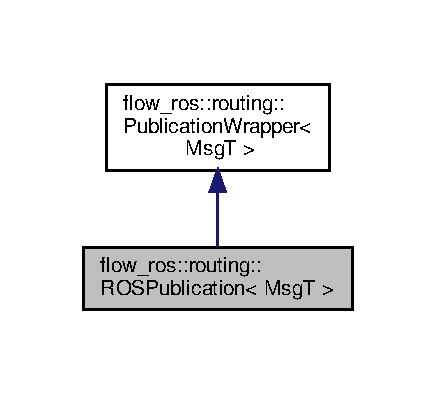
\includegraphics[width=209pt]{classflow__ros_1_1routing_1_1_r_o_s_publication__inherit__graph}
\end{center}
\end{figure}


Collaboration diagram for flow\+\_\+ros\+:\+:routing\+:\+:R\+O\+S\+Publication$<$ MsgT $>$\+:\nopagebreak
\begin{figure}[H]
\begin{center}
\leavevmode
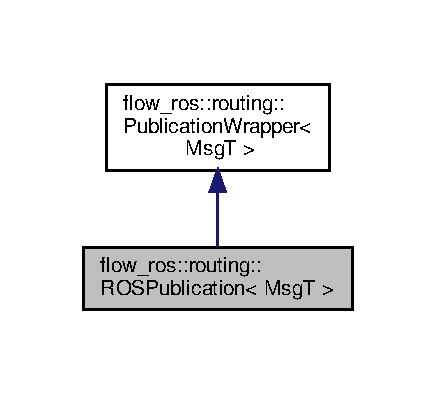
\includegraphics[width=209pt]{classflow__ros_1_1routing_1_1_r_o_s_publication__coll__graph}
\end{center}
\end{figure}
\subsection*{Public Member Functions}
\begin{DoxyCompactItemize}
\item 
\hyperlink{classflow__ros_1_1routing_1_1_r_o_s_publication_a78988f8588dc65e7e6b97dcb89b3f32a}{R\+O\+S\+Publication} (const ros\+::\+Publisher \&pub)
\begin{DoxyCompactList}\small\item\em R\+OS publisher constructor. \end{DoxyCompactList}\item 
void \hyperlink{classflow__ros_1_1routing_1_1_r_o_s_publication_a1ad3cf68c465a909399bb4496e561f0b}{publish} (const \hyperlink{namespaceflow__ros_a21a684f38ee2083b3858613317c46d82}{message\+\_\+shared\+\_\+ptr\+\_\+t}$<$ MsgT $>$ \&message) const override
\begin{DoxyCompactList}\small\item\em Call all held subscriber callbacks on message being published. \end{DoxyCompactList}\item 
std\+::string \hyperlink{classflow__ros_1_1routing_1_1_r_o_s_publication_a283e0832b79e8b1167d5e46bcde49c0b}{get\+Topic} () const override
\begin{DoxyCompactList}\small\item\em Returns topic associated with publication. \end{DoxyCompactList}\item 
std\+::uint32\+\_\+t \hyperlink{classflow__ros_1_1routing_1_1_r_o_s_publication_a2f7dac08ffdaab4942dde41f6e5b39ba}{get\+Num\+Subscribers} () const override
\begin{DoxyCompactList}\small\item\em Returns number of subscriptions connected to this publication. \end{DoxyCompactList}\item 
bool \hyperlink{classflow__ros_1_1routing_1_1_r_o_s_publication_a1abd966d244c71911a75a20a089025bc}{is\+Latched} () const override
\begin{DoxyCompactList}\small\item\em Returns flag indicating whether or not publisher is latched. \end{DoxyCompactList}\item 
\hyperlink{transport__info_8h_ae57afcf849a5bdb82b958347c6ccc57b}{Transport\+Method} \hyperlink{classflow__ros_1_1routing_1_1_r_o_s_publication_a2f2f880c127e4115d7edb85fb7faa067}{get\+Transport\+Method} () const override
\begin{DoxyCompactList}\small\item\em Returns transport method (code) associated with this publication. \end{DoxyCompactList}\item 
bool \hyperlink{classflow__ros_1_1routing_1_1_r_o_s_publication_aa7a132708199fe33bbb1420211aa7f78}{is\+Valid} () const override
\begin{DoxyCompactList}\small\item\em Validity check. \end{DoxyCompactList}\end{DoxyCompactItemize}
\subsection*{Additional Inherited Members}


\subsection{Detailed Description}
\subsubsection*{template$<$typename MsgT$>$\newline
class flow\+\_\+ros\+::routing\+::\+R\+O\+S\+Publication$<$ Msg\+T $>$}

Wrapper object for a {\ttfamily ros\+::\+Publisher} 


\begin{DoxyTemplParams}{Template Parameters}
{\em MsgT} & message data resource type \\
\hline
\end{DoxyTemplParams}


\subsection{Constructor \& Destructor Documentation}
\mbox{\Hypertarget{classflow__ros_1_1routing_1_1_r_o_s_publication_a78988f8588dc65e7e6b97dcb89b3f32a}\label{classflow__ros_1_1routing_1_1_r_o_s_publication_a78988f8588dc65e7e6b97dcb89b3f32a}} 
\index{flow\+\_\+ros\+::routing\+::\+R\+O\+S\+Publication@{flow\+\_\+ros\+::routing\+::\+R\+O\+S\+Publication}!R\+O\+S\+Publication@{R\+O\+S\+Publication}}
\index{R\+O\+S\+Publication@{R\+O\+S\+Publication}!flow\+\_\+ros\+::routing\+::\+R\+O\+S\+Publication@{flow\+\_\+ros\+::routing\+::\+R\+O\+S\+Publication}}
\subsubsection{\texorpdfstring{R\+O\+S\+Publication()}{ROSPublication()}}
{\footnotesize\ttfamily template$<$typename MsgT $>$ \\
\hyperlink{classflow__ros_1_1routing_1_1_r_o_s_publication}{flow\+\_\+ros\+::routing\+::\+R\+O\+S\+Publication}$<$ MsgT $>$\+::\hyperlink{classflow__ros_1_1routing_1_1_r_o_s_publication}{R\+O\+S\+Publication} (\begin{DoxyParamCaption}\item[{const ros\+::\+Publisher \&}]{pub }\end{DoxyParamCaption})\hspace{0.3cm}{\ttfamily [inline]}, {\ttfamily [explicit]}}



R\+OS publisher constructor. 


\begin{DoxyParams}{Parameters}
{\em pub} & R\+OS publisher encapsulation object \\
\hline
\end{DoxyParams}


\subsection{Member Function Documentation}
\mbox{\Hypertarget{classflow__ros_1_1routing_1_1_r_o_s_publication_a2f7dac08ffdaab4942dde41f6e5b39ba}\label{classflow__ros_1_1routing_1_1_r_o_s_publication_a2f7dac08ffdaab4942dde41f6e5b39ba}} 
\index{flow\+\_\+ros\+::routing\+::\+R\+O\+S\+Publication@{flow\+\_\+ros\+::routing\+::\+R\+O\+S\+Publication}!get\+Num\+Subscribers@{get\+Num\+Subscribers}}
\index{get\+Num\+Subscribers@{get\+Num\+Subscribers}!flow\+\_\+ros\+::routing\+::\+R\+O\+S\+Publication@{flow\+\_\+ros\+::routing\+::\+R\+O\+S\+Publication}}
\subsubsection{\texorpdfstring{get\+Num\+Subscribers()}{getNumSubscribers()}}
{\footnotesize\ttfamily template$<$typename MsgT $>$ \\
std\+::uint32\+\_\+t \hyperlink{classflow__ros_1_1routing_1_1_r_o_s_publication}{flow\+\_\+ros\+::routing\+::\+R\+O\+S\+Publication}$<$ MsgT $>$\+::get\+Num\+Subscribers (\begin{DoxyParamCaption}{ }\end{DoxyParamCaption}) const\hspace{0.3cm}{\ttfamily [inline]}, {\ttfamily [override]}, {\ttfamily [virtual]}}



Returns number of subscriptions connected to this publication. 



Implements \hyperlink{classflow__ros_1_1routing_1_1_publication_wrapper_a3e2fb2a4cafe729a643af5ed5033dc50}{flow\+\_\+ros\+::routing\+::\+Publication\+Wrapper$<$ Msg\+T $>$}.

\mbox{\Hypertarget{classflow__ros_1_1routing_1_1_r_o_s_publication_a283e0832b79e8b1167d5e46bcde49c0b}\label{classflow__ros_1_1routing_1_1_r_o_s_publication_a283e0832b79e8b1167d5e46bcde49c0b}} 
\index{flow\+\_\+ros\+::routing\+::\+R\+O\+S\+Publication@{flow\+\_\+ros\+::routing\+::\+R\+O\+S\+Publication}!get\+Topic@{get\+Topic}}
\index{get\+Topic@{get\+Topic}!flow\+\_\+ros\+::routing\+::\+R\+O\+S\+Publication@{flow\+\_\+ros\+::routing\+::\+R\+O\+S\+Publication}}
\subsubsection{\texorpdfstring{get\+Topic()}{getTopic()}}
{\footnotesize\ttfamily template$<$typename MsgT $>$ \\
std\+::string \hyperlink{classflow__ros_1_1routing_1_1_r_o_s_publication}{flow\+\_\+ros\+::routing\+::\+R\+O\+S\+Publication}$<$ MsgT $>$\+::get\+Topic (\begin{DoxyParamCaption}{ }\end{DoxyParamCaption}) const\hspace{0.3cm}{\ttfamily [inline]}, {\ttfamily [override]}, {\ttfamily [virtual]}}



Returns topic associated with publication. 



Implements \hyperlink{classflow__ros_1_1routing_1_1_publication_wrapper_a1aa441bb1846211cb803362233d4ee0b}{flow\+\_\+ros\+::routing\+::\+Publication\+Wrapper$<$ Msg\+T $>$}.

\mbox{\Hypertarget{classflow__ros_1_1routing_1_1_r_o_s_publication_a2f2f880c127e4115d7edb85fb7faa067}\label{classflow__ros_1_1routing_1_1_r_o_s_publication_a2f2f880c127e4115d7edb85fb7faa067}} 
\index{flow\+\_\+ros\+::routing\+::\+R\+O\+S\+Publication@{flow\+\_\+ros\+::routing\+::\+R\+O\+S\+Publication}!get\+Transport\+Method@{get\+Transport\+Method}}
\index{get\+Transport\+Method@{get\+Transport\+Method}!flow\+\_\+ros\+::routing\+::\+R\+O\+S\+Publication@{flow\+\_\+ros\+::routing\+::\+R\+O\+S\+Publication}}
\subsubsection{\texorpdfstring{get\+Transport\+Method()}{getTransportMethod()}}
{\footnotesize\ttfamily template$<$typename MsgT $>$ \\
\hyperlink{transport__info_8h_ae57afcf849a5bdb82b958347c6ccc57b}{Transport\+Method} \hyperlink{classflow__ros_1_1routing_1_1_r_o_s_publication}{flow\+\_\+ros\+::routing\+::\+R\+O\+S\+Publication}$<$ MsgT $>$\+::get\+Transport\+Method (\begin{DoxyParamCaption}{ }\end{DoxyParamCaption}) const\hspace{0.3cm}{\ttfamily [inline]}, {\ttfamily [override]}, {\ttfamily [virtual]}}



Returns transport method (code) associated with this publication. 



Implements \hyperlink{classflow__ros_1_1routing_1_1_publication_wrapper_a0398202c79a6bdb1ff57acc8c730bc65}{flow\+\_\+ros\+::routing\+::\+Publication\+Wrapper$<$ Msg\+T $>$}.

\mbox{\Hypertarget{classflow__ros_1_1routing_1_1_r_o_s_publication_a1abd966d244c71911a75a20a089025bc}\label{classflow__ros_1_1routing_1_1_r_o_s_publication_a1abd966d244c71911a75a20a089025bc}} 
\index{flow\+\_\+ros\+::routing\+::\+R\+O\+S\+Publication@{flow\+\_\+ros\+::routing\+::\+R\+O\+S\+Publication}!is\+Latched@{is\+Latched}}
\index{is\+Latched@{is\+Latched}!flow\+\_\+ros\+::routing\+::\+R\+O\+S\+Publication@{flow\+\_\+ros\+::routing\+::\+R\+O\+S\+Publication}}
\subsubsection{\texorpdfstring{is\+Latched()}{isLatched()}}
{\footnotesize\ttfamily template$<$typename MsgT $>$ \\
bool \hyperlink{classflow__ros_1_1routing_1_1_r_o_s_publication}{flow\+\_\+ros\+::routing\+::\+R\+O\+S\+Publication}$<$ MsgT $>$\+::is\+Latched (\begin{DoxyParamCaption}{ }\end{DoxyParamCaption}) const\hspace{0.3cm}{\ttfamily [inline]}, {\ttfamily [override]}, {\ttfamily [virtual]}}



Returns flag indicating whether or not publisher is latched. 



Implements \hyperlink{classflow__ros_1_1routing_1_1_publication_wrapper_a86fdc857e02347e862dbbb113e5a6cb6}{flow\+\_\+ros\+::routing\+::\+Publication\+Wrapper$<$ Msg\+T $>$}.

\mbox{\Hypertarget{classflow__ros_1_1routing_1_1_r_o_s_publication_aa7a132708199fe33bbb1420211aa7f78}\label{classflow__ros_1_1routing_1_1_r_o_s_publication_aa7a132708199fe33bbb1420211aa7f78}} 
\index{flow\+\_\+ros\+::routing\+::\+R\+O\+S\+Publication@{flow\+\_\+ros\+::routing\+::\+R\+O\+S\+Publication}!is\+Valid@{is\+Valid}}
\index{is\+Valid@{is\+Valid}!flow\+\_\+ros\+::routing\+::\+R\+O\+S\+Publication@{flow\+\_\+ros\+::routing\+::\+R\+O\+S\+Publication}}
\subsubsection{\texorpdfstring{is\+Valid()}{isValid()}}
{\footnotesize\ttfamily template$<$typename MsgT $>$ \\
bool \hyperlink{classflow__ros_1_1routing_1_1_r_o_s_publication}{flow\+\_\+ros\+::routing\+::\+R\+O\+S\+Publication}$<$ MsgT $>$\+::is\+Valid (\begin{DoxyParamCaption}{ }\end{DoxyParamCaption}) const\hspace{0.3cm}{\ttfamily [inline]}, {\ttfamily [override]}, {\ttfamily [virtual]}}



Validity check. 


\begin{DoxyRetVals}{Return values}
{\em true} & if underlying R\+OS publisher is valid \\
\hline
{\em false} & otherwise \\
\hline
\end{DoxyRetVals}


Implements \hyperlink{classflow__ros_1_1routing_1_1_publication_wrapper_afc33bf27092f8e8188e3f7955a6b7c97}{flow\+\_\+ros\+::routing\+::\+Publication\+Wrapper$<$ Msg\+T $>$}.

\mbox{\Hypertarget{classflow__ros_1_1routing_1_1_r_o_s_publication_a1ad3cf68c465a909399bb4496e561f0b}\label{classflow__ros_1_1routing_1_1_r_o_s_publication_a1ad3cf68c465a909399bb4496e561f0b}} 
\index{flow\+\_\+ros\+::routing\+::\+R\+O\+S\+Publication@{flow\+\_\+ros\+::routing\+::\+R\+O\+S\+Publication}!publish@{publish}}
\index{publish@{publish}!flow\+\_\+ros\+::routing\+::\+R\+O\+S\+Publication@{flow\+\_\+ros\+::routing\+::\+R\+O\+S\+Publication}}
\subsubsection{\texorpdfstring{publish()}{publish()}}
{\footnotesize\ttfamily template$<$typename MsgT $>$ \\
void \hyperlink{classflow__ros_1_1routing_1_1_r_o_s_publication}{flow\+\_\+ros\+::routing\+::\+R\+O\+S\+Publication}$<$ MsgT $>$\+::publish (\begin{DoxyParamCaption}\item[{const \hyperlink{namespaceflow__ros_a21a684f38ee2083b3858613317c46d82}{message\+\_\+shared\+\_\+ptr\+\_\+t}$<$ MsgT $>$ \&}]{message }\end{DoxyParamCaption}) const\hspace{0.3cm}{\ttfamily [inline]}, {\ttfamily [override]}, {\ttfamily [virtual]}}



Call all held subscriber callbacks on message being published. 


\begin{DoxyParams}{Parameters}
{\em message} & message data to publish \\
\hline
\end{DoxyParams}


Implements \hyperlink{classflow__ros_1_1routing_1_1_publication_wrapper_a43b9989390bf9f001fe9670a0c1d5897}{flow\+\_\+ros\+::routing\+::\+Publication\+Wrapper$<$ Msg\+T $>$}.



The documentation for this class was generated from the following file\+:\begin{DoxyCompactItemize}
\item 
flow\+\_\+ros/include/routing/ros\+\_\+publication.\+h\end{DoxyCompactItemize}

\hypertarget{classflow__ros_1_1routing_1_1_r_o_s_subscription}{}\section{flow\+\_\+ros\+:\+:routing\+:\+:R\+O\+S\+Subscription Class Reference}
\label{classflow__ros_1_1routing_1_1_r_o_s_subscription}\index{flow\+\_\+ros\+::routing\+::\+R\+O\+S\+Subscription@{flow\+\_\+ros\+::routing\+::\+R\+O\+S\+Subscription}}


Wrapper object for a {\ttfamily ros\+::\+Subscriber}  




{\ttfamily \#include $<$ros\+\_\+subscription.\+h$>$}



Inheritance diagram for flow\+\_\+ros\+:\+:routing\+:\+:R\+O\+S\+Subscription\+:\nopagebreak
\begin{figure}[H]
\begin{center}
\leavevmode
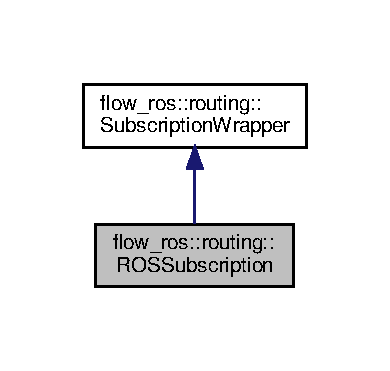
\includegraphics[width=187pt]{classflow__ros_1_1routing_1_1_r_o_s_subscription__inherit__graph}
\end{center}
\end{figure}


Collaboration diagram for flow\+\_\+ros\+:\+:routing\+:\+:R\+O\+S\+Subscription\+:\nopagebreak
\begin{figure}[H]
\begin{center}
\leavevmode
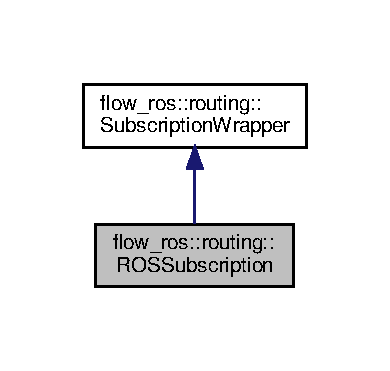
\includegraphics[width=187pt]{classflow__ros_1_1routing_1_1_r_o_s_subscription__coll__graph}
\end{center}
\end{figure}
\subsection*{Public Member Functions}
\begin{DoxyCompactItemize}
\item 
\hyperlink{classflow__ros_1_1routing_1_1_r_o_s_subscription_a8223b1ebd0550e650a53c8593a524253}{R\+O\+S\+Subscription} (const ros\+::\+Subscriber \&sub)
\begin{DoxyCompactList}\small\item\em R\+OS subscription constructor. \end{DoxyCompactList}\item 
std\+::string \hyperlink{classflow__ros_1_1routing_1_1_r_o_s_subscription_a3bdbb4897a1a8bdb67af2f72fb7645a7}{get\+Topic} () const override
\begin{DoxyCompactList}\small\item\em Returns topic associated with publication. \end{DoxyCompactList}\item 
std\+::uint32\+\_\+t \hyperlink{classflow__ros_1_1routing_1_1_r_o_s_subscription_a90b710d0cd089f60a3a2549acae6e8cb}{get\+Num\+Publishers} () const override
\begin{DoxyCompactList}\small\item\em Returns number of local publications connected to this subscription. \end{DoxyCompactList}\item 
\hyperlink{transport__info_8h_ae57afcf849a5bdb82b958347c6ccc57b}{Transport\+Method} \hyperlink{classflow__ros_1_1routing_1_1_r_o_s_subscription_a3dc2cff4348f072352a307c6902d1a18}{get\+Transport\+Method} () const override
\begin{DoxyCompactList}\small\item\em Returns transport method (code) associated with this subscription. \end{DoxyCompactList}\item 
bool \hyperlink{classflow__ros_1_1routing_1_1_r_o_s_subscription_a5f845fe965a9b166b02a87ffbb00e6ac}{is\+Valid} () const override
\begin{DoxyCompactList}\small\item\em Validity check. \end{DoxyCompactList}\end{DoxyCompactItemize}
\subsection*{Additional Inherited Members}


\subsection{Detailed Description}
Wrapper object for a {\ttfamily ros\+::\+Subscriber} 

\subsection{Constructor \& Destructor Documentation}
\mbox{\Hypertarget{classflow__ros_1_1routing_1_1_r_o_s_subscription_a8223b1ebd0550e650a53c8593a524253}\label{classflow__ros_1_1routing_1_1_r_o_s_subscription_a8223b1ebd0550e650a53c8593a524253}} 
\index{flow\+\_\+ros\+::routing\+::\+R\+O\+S\+Subscription@{flow\+\_\+ros\+::routing\+::\+R\+O\+S\+Subscription}!R\+O\+S\+Subscription@{R\+O\+S\+Subscription}}
\index{R\+O\+S\+Subscription@{R\+O\+S\+Subscription}!flow\+\_\+ros\+::routing\+::\+R\+O\+S\+Subscription@{flow\+\_\+ros\+::routing\+::\+R\+O\+S\+Subscription}}
\subsubsection{\texorpdfstring{R\+O\+S\+Subscription()}{ROSSubscription()}}
{\footnotesize\ttfamily flow\+\_\+ros\+::routing\+::\+R\+O\+S\+Subscription\+::\+R\+O\+S\+Subscription (\begin{DoxyParamCaption}\item[{const ros\+::\+Subscriber \&}]{sub }\end{DoxyParamCaption})\hspace{0.3cm}{\ttfamily [inline]}, {\ttfamily [explicit]}}



R\+OS subscription constructor. 


\begin{DoxyParams}{Parameters}
{\em sub} & R\+OS subscription encapsulation object \\
\hline
\end{DoxyParams}


\subsection{Member Function Documentation}
\mbox{\Hypertarget{classflow__ros_1_1routing_1_1_r_o_s_subscription_a90b710d0cd089f60a3a2549acae6e8cb}\label{classflow__ros_1_1routing_1_1_r_o_s_subscription_a90b710d0cd089f60a3a2549acae6e8cb}} 
\index{flow\+\_\+ros\+::routing\+::\+R\+O\+S\+Subscription@{flow\+\_\+ros\+::routing\+::\+R\+O\+S\+Subscription}!get\+Num\+Publishers@{get\+Num\+Publishers}}
\index{get\+Num\+Publishers@{get\+Num\+Publishers}!flow\+\_\+ros\+::routing\+::\+R\+O\+S\+Subscription@{flow\+\_\+ros\+::routing\+::\+R\+O\+S\+Subscription}}
\subsubsection{\texorpdfstring{get\+Num\+Publishers()}{getNumPublishers()}}
{\footnotesize\ttfamily std\+::uint32\+\_\+t flow\+\_\+ros\+::routing\+::\+R\+O\+S\+Subscription\+::get\+Num\+Publishers (\begin{DoxyParamCaption}{ }\end{DoxyParamCaption}) const\hspace{0.3cm}{\ttfamily [inline]}, {\ttfamily [override]}, {\ttfamily [virtual]}}



Returns number of local publications connected to this subscription. 



Implements \hyperlink{classflow__ros_1_1routing_1_1_subscription_wrapper_a8ae55d34a07c505dc2b4bcb2440b2d32}{flow\+\_\+ros\+::routing\+::\+Subscription\+Wrapper}.

\mbox{\Hypertarget{classflow__ros_1_1routing_1_1_r_o_s_subscription_a3bdbb4897a1a8bdb67af2f72fb7645a7}\label{classflow__ros_1_1routing_1_1_r_o_s_subscription_a3bdbb4897a1a8bdb67af2f72fb7645a7}} 
\index{flow\+\_\+ros\+::routing\+::\+R\+O\+S\+Subscription@{flow\+\_\+ros\+::routing\+::\+R\+O\+S\+Subscription}!get\+Topic@{get\+Topic}}
\index{get\+Topic@{get\+Topic}!flow\+\_\+ros\+::routing\+::\+R\+O\+S\+Subscription@{flow\+\_\+ros\+::routing\+::\+R\+O\+S\+Subscription}}
\subsubsection{\texorpdfstring{get\+Topic()}{getTopic()}}
{\footnotesize\ttfamily std\+::string flow\+\_\+ros\+::routing\+::\+R\+O\+S\+Subscription\+::get\+Topic (\begin{DoxyParamCaption}{ }\end{DoxyParamCaption}) const\hspace{0.3cm}{\ttfamily [inline]}, {\ttfamily [override]}, {\ttfamily [virtual]}}



Returns topic associated with publication. 



Implements \hyperlink{classflow__ros_1_1routing_1_1_subscription_wrapper_a2ef27475e7b7d7555e90d02cdc220b88}{flow\+\_\+ros\+::routing\+::\+Subscription\+Wrapper}.

\mbox{\Hypertarget{classflow__ros_1_1routing_1_1_r_o_s_subscription_a3dc2cff4348f072352a307c6902d1a18}\label{classflow__ros_1_1routing_1_1_r_o_s_subscription_a3dc2cff4348f072352a307c6902d1a18}} 
\index{flow\+\_\+ros\+::routing\+::\+R\+O\+S\+Subscription@{flow\+\_\+ros\+::routing\+::\+R\+O\+S\+Subscription}!get\+Transport\+Method@{get\+Transport\+Method}}
\index{get\+Transport\+Method@{get\+Transport\+Method}!flow\+\_\+ros\+::routing\+::\+R\+O\+S\+Subscription@{flow\+\_\+ros\+::routing\+::\+R\+O\+S\+Subscription}}
\subsubsection{\texorpdfstring{get\+Transport\+Method()}{getTransportMethod()}}
{\footnotesize\ttfamily \hyperlink{transport__info_8h_ae57afcf849a5bdb82b958347c6ccc57b}{Transport\+Method} flow\+\_\+ros\+::routing\+::\+R\+O\+S\+Subscription\+::get\+Transport\+Method (\begin{DoxyParamCaption}{ }\end{DoxyParamCaption}) const\hspace{0.3cm}{\ttfamily [inline]}, {\ttfamily [override]}, {\ttfamily [virtual]}}



Returns transport method (code) associated with this subscription. 



Implements \hyperlink{classflow__ros_1_1routing_1_1_subscription_wrapper_a063fcc10600ef657620e2b58ce1fca85}{flow\+\_\+ros\+::routing\+::\+Subscription\+Wrapper}.

\mbox{\Hypertarget{classflow__ros_1_1routing_1_1_r_o_s_subscription_a5f845fe965a9b166b02a87ffbb00e6ac}\label{classflow__ros_1_1routing_1_1_r_o_s_subscription_a5f845fe965a9b166b02a87ffbb00e6ac}} 
\index{flow\+\_\+ros\+::routing\+::\+R\+O\+S\+Subscription@{flow\+\_\+ros\+::routing\+::\+R\+O\+S\+Subscription}!is\+Valid@{is\+Valid}}
\index{is\+Valid@{is\+Valid}!flow\+\_\+ros\+::routing\+::\+R\+O\+S\+Subscription@{flow\+\_\+ros\+::routing\+::\+R\+O\+S\+Subscription}}
\subsubsection{\texorpdfstring{is\+Valid()}{isValid()}}
{\footnotesize\ttfamily bool flow\+\_\+ros\+::routing\+::\+R\+O\+S\+Subscription\+::is\+Valid (\begin{DoxyParamCaption}{ }\end{DoxyParamCaption}) const\hspace{0.3cm}{\ttfamily [inline]}, {\ttfamily [override]}, {\ttfamily [virtual]}}



Validity check. 


\begin{DoxyRetVals}{Return values}
{\em true} & if underlying R\+OS subscriber is valid \\
\hline
{\em false} & otherwise \\
\hline
\end{DoxyRetVals}


Implements \hyperlink{classflow__ros_1_1routing_1_1_subscription_wrapper_a0f23052807c3533d28168d7c681a221e}{flow\+\_\+ros\+::routing\+::\+Subscription\+Wrapper}.



The documentation for this class was generated from the following file\+:\begin{DoxyCompactItemize}
\item 
flow\+\_\+ros/include/routing/ros\+\_\+subscription.\+h\end{DoxyCompactItemize}

\hypertarget{classflow__ros_1_1_router}{}\section{flow\+\_\+ros\+:\+:Router Class Reference}
\label{classflow__ros_1_1_router}\index{flow\+\_\+ros\+::\+Router@{flow\+\_\+ros\+::\+Router}}


An in-\/process message routing object.  




{\ttfamily \#include $<$router.\+h$>$}

\subsection*{Public Member Functions}
\begin{DoxyCompactItemize}
\item 
\hyperlink{classflow__ros_1_1_router_a90b7c5099932b00dee22ed58c99644a0}{Router} (std\+::string ns=\char`\"{}anonymous\+\_\+local\+\_\+context\char`\"{})
\begin{DoxyCompactList}\small\item\em Namespace constructor. \end{DoxyCompactList}\item 
\mbox{\Hypertarget{classflow__ros_1_1_router_a8192fca645e648bba809fc1975fbe261}\label{classflow__ros_1_1_router_a8192fca645e648bba809fc1975fbe261}} 
const std\+::string \& \hyperlink{classflow__ros_1_1_router_a8192fca645e648bba809fc1975fbe261}{get\+Namespace} () const
\begin{DoxyCompactList}\small\item\em Returns name associated with this \hyperlink{classflow__ros_1_1_router}{Router}. \end{DoxyCompactList}\item 
\mbox{\Hypertarget{classflow__ros_1_1_router_a53f2dc6ff8226ac8cf60af80123596db}\label{classflow__ros_1_1_router_a53f2dc6ff8226ac8cf60af80123596db}} 
void \hyperlink{classflow__ros_1_1_router_a53f2dc6ff8226ac8cf60af80123596db}{clear} ()
\begin{DoxyCompactList}\small\item\em Clears all known subscriptions and publications. \end{DoxyCompactList}\item 
{\footnotesize template$<$typename MsgT $>$ }\\std\+::shared\+\_\+ptr$<$ \hyperlink{classflow__ros_1_1routing_1_1_local_publication}{publication\+\_\+t}$<$ MsgT $>$ $>$ \hyperlink{classflow__ros_1_1_router_a9063ea60d71047f372d7321f36629ca4}{advertise} (const std\+::string \&topic, const std\+::uint32\+\_\+t queue\+\_\+size, bool latch=false)
\begin{DoxyCompactList}\small\item\em Advertises a new local Publication. \end{DoxyCompactList}\item 
{\footnotesize template$<$typename MsgT , typename CallbackT $>$ }\\std\+::shared\+\_\+ptr$<$ \hyperlink{classflow__ros_1_1routing_1_1_local_subscription}{subscription\+\_\+t}$<$ MsgT $>$ $>$ \hyperlink{classflow__ros_1_1_router_a6f8d999bfe280549f4a3216205007450}{subscribe} (const std\+::string \&topic, const std\+::uint32\+\_\+t queue\+\_\+size, CallbackT \&\&callback)
\begin{DoxyCompactList}\small\item\em Creates a new local Subscription. \end{DoxyCompactList}\item 
{\footnotesize template$<$typename MsgT , typename MethodT , typename ThisT $>$ }\\std\+::shared\+\_\+ptr$<$ \hyperlink{classflow__ros_1_1routing_1_1_local_subscription}{subscription\+\_\+t}$<$ MsgT $>$ $>$ \hyperlink{classflow__ros_1_1_router_a00e52e1f0df24ff0ca4b2f80d5b6fd0d}{subscribe} (const std\+::string \&topic, const std\+::uint32\+\_\+t queue\+\_\+size, MethodT \&\&m\+\_\+fn\+\_\+ptr, ThisT \&\&this\+\_\+ptr)
\begin{DoxyCompactList}\small\item\em Creates a new local Subscription. \end{DoxyCompactList}\item 
{\footnotesize template$<$typename MsgT , template$<$ typename $>$ class Shared\+Ptr\+Tmpl$>$ }\\void \hyperlink{classflow__ros_1_1_router_ae41d76f1feb66cd4302172d42253454c}{inject} (const std\+::string \&topic, const Shared\+Ptr\+Tmpl$<$ MsgT $>$ \&msg)
\begin{DoxyCompactList}\small\item\em Inject message on a given topic. \end{DoxyCompactList}\item 
void \hyperlink{classflow__ros_1_1_router_a9a6615abdc9e1091c73acc86fcbf795c}{inject} (const \+::rosbag\+::\+Message\+Instance \&mi)
\begin{DoxyCompactList}\small\item\em Inject R\+OS bag message instance on a given topic. \end{DoxyCompactList}\item 
\mbox{\Hypertarget{classflow__ros_1_1_router_ab191406d34d07cd14ecfc484b501fe52}\label{classflow__ros_1_1_router_ab191406d34d07cd14ecfc484b501fe52}} 
std\+::vector$<$ std\+::string $>$ \hyperlink{classflow__ros_1_1_router_ab191406d34d07cd14ecfc484b501fe52}{known\+Publications} () const
\begin{DoxyCompactList}\small\item\em Returns a vector of known published topics. \end{DoxyCompactList}\item 
\mbox{\Hypertarget{classflow__ros_1_1_router_abf8bb94e109ee8b0987aa50e35721874}\label{classflow__ros_1_1_router_abf8bb94e109ee8b0987aa50e35721874}} 
std\+::vector$<$ std\+::string $>$ \hyperlink{classflow__ros_1_1_router_abf8bb94e109ee8b0987aa50e35721874}{known\+Subscriptions} () const
\begin{DoxyCompactList}\small\item\em Returns a vector of known subscribed topics. \end{DoxyCompactList}\item 
std\+::string \hyperlink{classflow__ros_1_1_router_a3674f0a63ecdaed3619c6edeffa1b484}{resolve\+Name} (const std\+::string \&topic) const
\begin{DoxyCompactList}\small\item\em Returns topic name resolved under \hyperlink{classflow__ros_1_1_router}{Router} namespace. \end{DoxyCompactList}\end{DoxyCompactItemize}
\subsection*{Friends}
\begin{DoxyCompactItemize}
\item 
std\+::ostream \& \hyperlink{classflow__ros_1_1_router_a78e8ba9cec95e91e9abe6d8f83375feb}{operator$<$$<$} (std\+::ostream \&os, const \hyperlink{classflow__ros_1_1_router}{Router} \&router)
\begin{DoxyCompactList}\small\item\em \hyperlink{classflow__ros_1_1_router}{Router} output stream operator overload. \end{DoxyCompactList}\end{DoxyCompactItemize}


\subsection{Detailed Description}
An in-\/process message routing object. 

Can advertise and subscribe to message topics, and matches connection-\/making interfaces of a {\ttfamily ros\+::\+Node\+Handle$<$code$>$. Allows for the ability to connect {\ttfamily Event\+Handlers$<$/code in-\/process with data channels that do not pass R\+O\+S-\/serializable messages }}

\subsection{Constructor \& Destructor Documentation}
\mbox{\Hypertarget{classflow__ros_1_1_router_a90b7c5099932b00dee22ed58c99644a0}\label{classflow__ros_1_1_router_a90b7c5099932b00dee22ed58c99644a0}} 
\index{flow\+\_\+ros\+::\+Router@{flow\+\_\+ros\+::\+Router}!Router@{Router}}
\index{Router@{Router}!flow\+\_\+ros\+::\+Router@{flow\+\_\+ros\+::\+Router}}
\subsubsection{\texorpdfstring{Router()}{Router()}}
{\footnotesize\ttfamily flow\+\_\+ros\+::\+Router\+::\+Router (\begin{DoxyParamCaption}\item[{std\+::string}]{ns = {\ttfamily \char`\"{}anonymous\+\_\+local\+\_\+context\char`\"{}} }\end{DoxyParamCaption})\hspace{0.3cm}{\ttfamily [explicit]}}



Namespace constructor. 


\begin{DoxyParams}{Parameters}
{\em ns} & namespace to associated with this \hyperlink{classflow__ros_1_1_router}{Router} \\
\hline
\end{DoxyParams}


\subsection{Member Function Documentation}
\mbox{\Hypertarget{classflow__ros_1_1_router_a9063ea60d71047f372d7321f36629ca4}\label{classflow__ros_1_1_router_a9063ea60d71047f372d7321f36629ca4}} 
\index{flow\+\_\+ros\+::\+Router@{flow\+\_\+ros\+::\+Router}!advertise@{advertise}}
\index{advertise@{advertise}!flow\+\_\+ros\+::\+Router@{flow\+\_\+ros\+::\+Router}}
\subsubsection{\texorpdfstring{advertise()}{advertise()}}
{\footnotesize\ttfamily template$<$typename MsgT $>$ \\
std\+::shared\+\_\+ptr$<$\hyperlink{classflow__ros_1_1routing_1_1_local_publication}{publication\+\_\+t}$<$MsgT$>$ $>$ flow\+\_\+ros\+::\+Router\+::advertise (\begin{DoxyParamCaption}\item[{const std\+::string \&}]{topic,  }\item[{const std\+::uint32\+\_\+t}]{queue\+\_\+size,  }\item[{bool}]{latch = {\ttfamily false} }\end{DoxyParamCaption})\hspace{0.3cm}{\ttfamily [inline]}}



Advertises a new local Publication. 


\begin{DoxyTemplParams}{Template Parameters}
{\em MsgT} & (deduced) type of message to be published\\
\hline
\end{DoxyTemplParams}

\begin{DoxyParams}{Parameters}
{\em topic} & topic associated with messages to publish \\
\hline
{\em queue\+\_\+size} & unused \\
\hline
{\em latch} & unused\\
\hline
\end{DoxyParams}
\begin{DoxyReturn}{Returns}
new Publication resource 
\end{DoxyReturn}
\mbox{\Hypertarget{classflow__ros_1_1_router_ae41d76f1feb66cd4302172d42253454c}\label{classflow__ros_1_1_router_ae41d76f1feb66cd4302172d42253454c}} 
\index{flow\+\_\+ros\+::\+Router@{flow\+\_\+ros\+::\+Router}!inject@{inject}}
\index{inject@{inject}!flow\+\_\+ros\+::\+Router@{flow\+\_\+ros\+::\+Router}}
\subsubsection{\texorpdfstring{inject()}{inject()}\hspace{0.1cm}{\footnotesize\ttfamily [1/2]}}
{\footnotesize\ttfamily template$<$typename MsgT , template$<$ typename $>$ class Shared\+Ptr\+Tmpl$>$ \\
void flow\+\_\+ros\+::\+Router\+::inject (\begin{DoxyParamCaption}\item[{const std\+::string \&}]{topic,  }\item[{const Shared\+Ptr\+Tmpl$<$ MsgT $>$ \&}]{msg }\end{DoxyParamCaption})\hspace{0.3cm}{\ttfamily [inline]}}



Inject message on a given topic. 


\begin{DoxyTemplParams}{Template Parameters}
{\em MsgT} & (deduced) type of message to inject \\
\hline
{\em Shared\+Ptr\+Tmpl} & (deduced) share pointer object template\\
\hline
\end{DoxyTemplParams}

\begin{DoxyParams}{Parameters}
{\em topic} & name of local topic to publish on \\
\hline
{\em msg} & message to inject to input (subscription) channel for given topic\\
\hline
\end{DoxyParams}

\begin{DoxyExceptions}{Exceptions}
{\em $<$code$>$\+Unknown\+Subscription\+Error$<$/code$>$} & if there is no subscription for given topic \\
\hline
\end{DoxyExceptions}
\mbox{\Hypertarget{classflow__ros_1_1_router_a9a6615abdc9e1091c73acc86fcbf795c}\label{classflow__ros_1_1_router_a9a6615abdc9e1091c73acc86fcbf795c}} 
\index{flow\+\_\+ros\+::\+Router@{flow\+\_\+ros\+::\+Router}!inject@{inject}}
\index{inject@{inject}!flow\+\_\+ros\+::\+Router@{flow\+\_\+ros\+::\+Router}}
\subsubsection{\texorpdfstring{inject()}{inject()}\hspace{0.1cm}{\footnotesize\ttfamily [2/2]}}
{\footnotesize\ttfamily void flow\+\_\+ros\+::\+Router\+::inject (\begin{DoxyParamCaption}\item[{const \+::rosbag\+::\+Message\+Instance \&}]{mi }\end{DoxyParamCaption})\hspace{0.3cm}{\ttfamily [inline]}}



Inject R\+OS bag message instance on a given topic. 


\begin{DoxyParams}{Parameters}
{\em mi} & R\+OS bag message instance\\
\hline
\end{DoxyParams}

\begin{DoxyExceptions}{Exceptions}
{\em $<$code$>$\+Unknown\+Subscription\+Error$<$/code$>$} & if there is no subscription for given topic \\
\hline
{\em $<$code$>$std\+::runtime\+\_\+error$<$/code$>$} & on failure to instance message \\
\hline
\end{DoxyExceptions}
\mbox{\Hypertarget{classflow__ros_1_1_router_a3674f0a63ecdaed3619c6edeffa1b484}\label{classflow__ros_1_1_router_a3674f0a63ecdaed3619c6edeffa1b484}} 
\index{flow\+\_\+ros\+::\+Router@{flow\+\_\+ros\+::\+Router}!resolve\+Name@{resolve\+Name}}
\index{resolve\+Name@{resolve\+Name}!flow\+\_\+ros\+::\+Router@{flow\+\_\+ros\+::\+Router}}
\subsubsection{\texorpdfstring{resolve\+Name()}{resolveName()}}
{\footnotesize\ttfamily std\+::string flow\+\_\+ros\+::\+Router\+::resolve\+Name (\begin{DoxyParamCaption}\item[{const std\+::string \&}]{topic }\end{DoxyParamCaption}) const}



Returns topic name resolved under \hyperlink{classflow__ros_1_1_router}{Router} namespace. 


\begin{DoxyParams}{Parameters}
{\em topic} & topic name to resolve\\
\hline
\end{DoxyParams}
\begin{DoxyReturn}{Returns}
resolved version of {\ttfamily topic} 
\end{DoxyReturn}

\begin{DoxyExceptions}{Exceptions}
{\em $<$code$>$std\+::invalid\+\_\+argument$<$/code$>$} & if {\ttfamily topic} is invalid \\
\hline
\end{DoxyExceptions}
\mbox{\Hypertarget{classflow__ros_1_1_router_a6f8d999bfe280549f4a3216205007450}\label{classflow__ros_1_1_router_a6f8d999bfe280549f4a3216205007450}} 
\index{flow\+\_\+ros\+::\+Router@{flow\+\_\+ros\+::\+Router}!subscribe@{subscribe}}
\index{subscribe@{subscribe}!flow\+\_\+ros\+::\+Router@{flow\+\_\+ros\+::\+Router}}
\subsubsection{\texorpdfstring{subscribe()}{subscribe()}\hspace{0.1cm}{\footnotesize\ttfamily [1/2]}}
{\footnotesize\ttfamily template$<$typename MsgT , typename CallbackT $>$ \\
std\+::shared\+\_\+ptr$<$\hyperlink{classflow__ros_1_1routing_1_1_local_subscription}{subscription\+\_\+t}$<$MsgT$>$ $>$ flow\+\_\+ros\+::\+Router\+::subscribe (\begin{DoxyParamCaption}\item[{const std\+::string \&}]{topic,  }\item[{const std\+::uint32\+\_\+t}]{queue\+\_\+size,  }\item[{CallbackT \&\&}]{callback }\end{DoxyParamCaption})\hspace{0.3cm}{\ttfamily [inline]}}



Creates a new local Subscription. 


\begin{DoxyTemplParams}{Template Parameters}
{\em MsgT} & (deduced) type of message to be received\\
\hline
\end{DoxyTemplParams}

\begin{DoxyParams}{Parameters}
{\em topic} & topic associated with messages to publish \\
\hline
{\em queue\+\_\+size} & unused \\
\hline
{\em cb} & message callback to associated with subscriber\\
\hline
\end{DoxyParams}
\begin{DoxyReturn}{Returns}
new Subscription resource 
\end{DoxyReturn}
\mbox{\Hypertarget{classflow__ros_1_1_router_a00e52e1f0df24ff0ca4b2f80d5b6fd0d}\label{classflow__ros_1_1_router_a00e52e1f0df24ff0ca4b2f80d5b6fd0d}} 
\index{flow\+\_\+ros\+::\+Router@{flow\+\_\+ros\+::\+Router}!subscribe@{subscribe}}
\index{subscribe@{subscribe}!flow\+\_\+ros\+::\+Router@{flow\+\_\+ros\+::\+Router}}
\subsubsection{\texorpdfstring{subscribe()}{subscribe()}\hspace{0.1cm}{\footnotesize\ttfamily [2/2]}}
{\footnotesize\ttfamily template$<$typename MsgT , typename MethodT , typename ThisT $>$ \\
std\+::shared\+\_\+ptr$<$\hyperlink{classflow__ros_1_1routing_1_1_local_subscription}{subscription\+\_\+t}$<$MsgT$>$ $>$ flow\+\_\+ros\+::\+Router\+::subscribe (\begin{DoxyParamCaption}\item[{const std\+::string \&}]{topic,  }\item[{const std\+::uint32\+\_\+t}]{queue\+\_\+size,  }\item[{MethodT \&\&}]{m\+\_\+fn\+\_\+ptr,  }\item[{ThisT \&\&}]{this\+\_\+ptr }\end{DoxyParamCaption})\hspace{0.3cm}{\ttfamily [inline]}}



Creates a new local Subscription. 

This is a convenience method for class methods


\begin{DoxyTemplParams}{Template Parameters}
{\em MsgT} & (deduced) type of message to be published \\
\hline
{\em MethodT} & (deduced) class method type \\
\hline
{\em ThisT} & (deduced) class pointer type\\
\hline
\end{DoxyTemplParams}

\begin{DoxyParams}{Parameters}
{\em topic} & topic associated with messages to publish \\
\hline
{\em queue\+\_\+size} & unused \\
\hline
{\em m\+\_\+fn\+\_\+ptr} & message callback to associated with subscriber \\
\hline
{\em this\+\_\+ptr} & object with method {\ttfamily m\+\_\+fn\+\_\+ptr}\\
\hline
\end{DoxyParams}
\begin{DoxyReturn}{Returns}
new Subscription resource 
\end{DoxyReturn}


\subsection{Friends And Related Function Documentation}
\mbox{\Hypertarget{classflow__ros_1_1_router_a78e8ba9cec95e91e9abe6d8f83375feb}\label{classflow__ros_1_1_router_a78e8ba9cec95e91e9abe6d8f83375feb}} 
\index{flow\+\_\+ros\+::\+Router@{flow\+\_\+ros\+::\+Router}!operator$<$$<$@{operator$<$$<$}}
\index{operator$<$$<$@{operator$<$$<$}!flow\+\_\+ros\+::\+Router@{flow\+\_\+ros\+::\+Router}}
\subsubsection{\texorpdfstring{operator$<$$<$}{operator<<}}
{\footnotesize\ttfamily std\+::ostream\& operator$<$$<$ (\begin{DoxyParamCaption}\item[{std\+::ostream \&}]{os,  }\item[{const \hyperlink{classflow__ros_1_1_router}{Router} \&}]{router }\end{DoxyParamCaption})\hspace{0.3cm}{\ttfamily [friend]}}



\hyperlink{classflow__ros_1_1_router}{Router} output stream operator overload. 


\begin{DoxyParams}[1]{Parameters}
\mbox{\tt in,out}  & {\em os} & output stream \\
\hline
 & {\em router} & router object\\
\hline
\end{DoxyParams}
\begin{DoxyReturn}{Returns}
os 
\end{DoxyReturn}


The documentation for this class was generated from the following files\+:\begin{DoxyCompactItemize}
\item 
flow\+\_\+ros/include/\hyperlink{router_8h}{router.\+h}\item 
flow\+\_\+ros/src/router.\+cpp\end{DoxyCompactItemize}

\hypertarget{structflow__ros_1_1_stamp_setter}{}\section{flow\+\_\+ros\+:\+:Stamp\+Setter$<$ MsgT $>$ Struct Template Reference}
\label{structflow__ros_1_1_stamp_setter}\index{flow\+\_\+ros\+::\+Stamp\+Setter$<$ Msg\+T $>$@{flow\+\_\+ros\+::\+Stamp\+Setter$<$ Msg\+T $>$}}


Helper object use to set message stamps.  




{\ttfamily \#include $<$message\+\_\+seq\+\_\+access.\+h$>$}

\subsection*{Public Member Functions}
\begin{DoxyCompactItemize}
\item 
\mbox{\Hypertarget{structflow__ros_1_1_stamp_setter_af507692487d1b9efe3c21c76a5351a6c}\label{structflow__ros_1_1_stamp_setter_af507692487d1b9efe3c21c76a5351a6c}} 
void {\bfseries operator()} (MsgT \&msg, std\+::uint32\+\_\+t seq) const
\item 
\mbox{\Hypertarget{structflow__ros_1_1_stamp_setter_a6cec19566ccce497e73240ef20db7fc1}\label{structflow__ros_1_1_stamp_setter_a6cec19566ccce497e73240ef20db7fc1}} 
void {\bfseries operator()} (MsgT \&msg, const ros\+::\+Time \&stamp) const
\end{DoxyCompactItemize}


\subsection{Detailed Description}
\subsubsection*{template$<$typename MsgT$>$\newline
struct flow\+\_\+ros\+::\+Stamp\+Setter$<$ Msg\+T $>$}

Helper object use to set message stamps. 


\begin{DoxyTemplParams}{Template Parameters}
{\em MsgT} & message type\\
\hline
\end{DoxyTemplParams}
\begin{DoxyNote}{Note}
May be specialized for any message with a sequence count
\end{DoxyNote}

\begin{DoxyTemplParams}{Template Parameters}
{\em MsgT} & message type\\
\hline
\end{DoxyTemplParams}
\begin{DoxyNote}{Note}
May be specialized for any message with a stamp 
\end{DoxyNote}


The documentation for this struct was generated from the following files\+:\begin{DoxyCompactItemize}
\item 
flow\+\_\+ros/include/\hyperlink{message__seq__access_8h}{message\+\_\+seq\+\_\+access.\+h}\item 
flow\+\_\+ros/include/\hyperlink{message__stamp__access_8h}{message\+\_\+stamp\+\_\+access.\+h}\end{DoxyCompactItemize}

\hypertarget{structflow_1_1_stamp_traits_3_01ros_1_1_time_01_4}{}\section{flow\+:\+:Stamp\+Traits$<$ ros\+:\+:Time $>$ Struct Template Reference}
\label{structflow_1_1_stamp_traits_3_01ros_1_1_time_01_4}\index{flow\+::\+Stamp\+Traits$<$ ros\+::\+Time $>$@{flow\+::\+Stamp\+Traits$<$ ros\+::\+Time $>$}}


R\+OS timing type traits for associated message Dispatch.  




{\ttfamily \#include $<$message\+\_\+stamp\+\_\+access.\+h$>$}

\subsection*{Public Types}
\begin{DoxyCompactItemize}
\item 
\mbox{\Hypertarget{structflow_1_1_stamp_traits_3_01ros_1_1_time_01_4_ab9356c00557c26b1e5447c75013a2a3f}\label{structflow_1_1_stamp_traits_3_01ros_1_1_time_01_4_ab9356c00557c26b1e5447c75013a2a3f}} 
using \hyperlink{structflow_1_1_stamp_traits_3_01ros_1_1_time_01_4_ab9356c00557c26b1e5447c75013a2a3f}{stamp\+\_\+type} = ros\+::\+Time
\begin{DoxyCompactList}\small\item\em Stamp type. \end{DoxyCompactList}\item 
\mbox{\Hypertarget{structflow_1_1_stamp_traits_3_01ros_1_1_time_01_4_a52fd431d0803e62cd978bf692c956c46}\label{structflow_1_1_stamp_traits_3_01ros_1_1_time_01_4_a52fd431d0803e62cd978bf692c956c46}} 
using \hyperlink{structflow_1_1_stamp_traits_3_01ros_1_1_time_01_4_a52fd431d0803e62cd978bf692c956c46}{offset\+\_\+type} = ros\+::\+Duration
\begin{DoxyCompactList}\small\item\em Associated duration/offset type. \end{DoxyCompactList}\end{DoxyCompactItemize}
\subsection*{Static Public Member Functions}
\begin{DoxyCompactItemize}
\item 
\mbox{\Hypertarget{structflow_1_1_stamp_traits_3_01ros_1_1_time_01_4_a984be4e6f28eb45d7f7b8f88a4ccf009}\label{structflow_1_1_stamp_traits_3_01ros_1_1_time_01_4_a984be4e6f28eb45d7f7b8f88a4ccf009}} 
static ros\+::\+Time \hyperlink{structflow_1_1_stamp_traits_3_01ros_1_1_time_01_4_a984be4e6f28eb45d7f7b8f88a4ccf009}{min} ()
\begin{DoxyCompactList}\small\item\em Returns minimum stamp value. \end{DoxyCompactList}\item 
\mbox{\Hypertarget{structflow_1_1_stamp_traits_3_01ros_1_1_time_01_4_ab2e686990f4e854ea6d343e5aa98cede}\label{structflow_1_1_stamp_traits_3_01ros_1_1_time_01_4_ab2e686990f4e854ea6d343e5aa98cede}} 
static ros\+::\+Time \hyperlink{structflow_1_1_stamp_traits_3_01ros_1_1_time_01_4_ab2e686990f4e854ea6d343e5aa98cede}{max} ()
\begin{DoxyCompactList}\small\item\em Returns maximum stamp value. \end{DoxyCompactList}\end{DoxyCompactItemize}


\subsection{Detailed Description}
\subsubsection*{template$<$$>$\newline
struct flow\+::\+Stamp\+Traits$<$ ros\+::\+Time $>$}

R\+OS timing type traits for associated message Dispatch. 

The documentation for this struct was generated from the following file\+:\begin{DoxyCompactItemize}
\item 
flow\+\_\+ros/include/\hyperlink{message__stamp__access_8h}{message\+\_\+stamp\+\_\+access.\+h}\end{DoxyCompactItemize}

\hypertarget{classflow__ros_1_1_subscriber}{}\section{flow\+\_\+ros\+:\+:Subscriber$<$ MsgT, Policy\+Tmpl, Lock\+PolicyT, Msg\+Const\+Ptr\+ContainerT $>$ Class Template Reference}
\label{classflow__ros_1_1_subscriber}\index{flow\+\_\+ros\+::\+Subscriber$<$ Msg\+T, Policy\+Tmpl, Lock\+Policy\+T, Msg\+Const\+Ptr\+Container\+T $>$@{flow\+\_\+ros\+::\+Subscriber$<$ Msg\+T, Policy\+Tmpl, Lock\+Policy\+T, Msg\+Const\+Ptr\+Container\+T $>$}}


Input channel which subscribes to messages.  




{\ttfamily \#include $<$subscriber.\+h$>$}



Inheritance diagram for flow\+\_\+ros\+:\+:Subscriber$<$ MsgT, Policy\+Tmpl, Lock\+PolicyT, Msg\+Const\+Ptr\+ContainerT $>$\+:\nopagebreak
\begin{figure}[H]
\begin{center}
\leavevmode
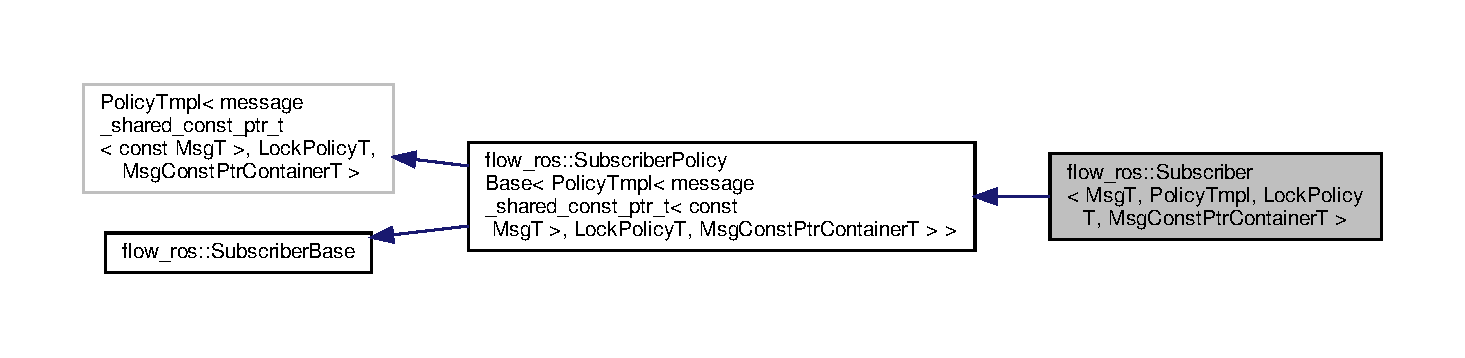
\includegraphics[width=350pt]{classflow__ros_1_1_subscriber__inherit__graph}
\end{center}
\end{figure}


Collaboration diagram for flow\+\_\+ros\+:\+:Subscriber$<$ MsgT, Policy\+Tmpl, Lock\+PolicyT, Msg\+Const\+Ptr\+ContainerT $>$\+:\nopagebreak
\begin{figure}[H]
\begin{center}
\leavevmode
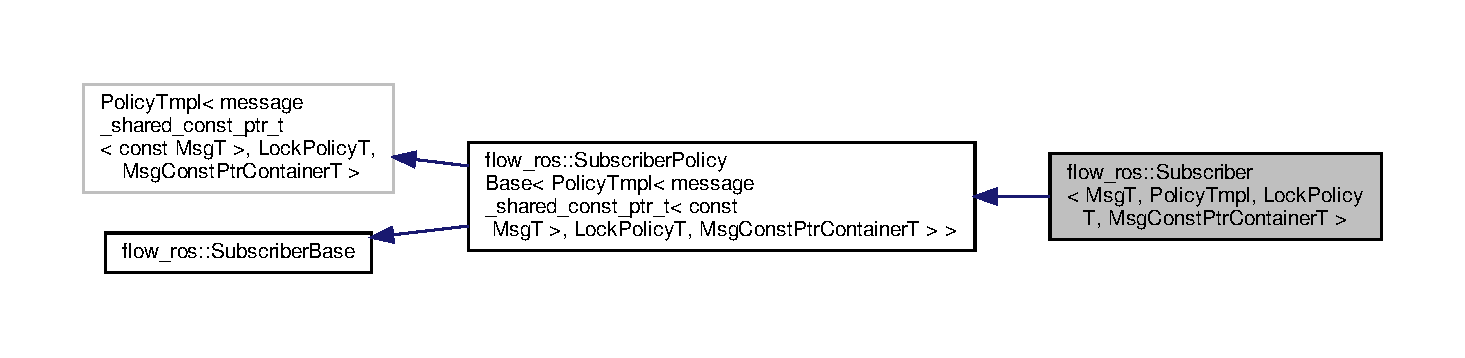
\includegraphics[width=350pt]{classflow__ros_1_1_subscriber__coll__graph}
\end{center}
\end{figure}
\subsection*{Public Member Functions}
\begin{DoxyCompactItemize}
\item 
{\footnotesize template$<$typename... Policy\+Arg\+Ts$>$ }\\\hyperlink{classflow__ros_1_1_subscriber_ae47148b0782dd9d38cd68b7860751fe6}{Subscriber} (ros\+::\+Node\+Handle \&nh, const std\+::string \&topic, const std\+::uint32\+\_\+t queue\+\_\+size, Policy\+Arg\+Ts \&\&... args)
\begin{DoxyCompactList}\small\item\em {\ttfamily ros\+::\+Node\+Handle} setup constructor (no transport hints) \end{DoxyCompactList}\item 
{\footnotesize template$<$typename... Policy\+Arg\+Ts$>$ }\\\hyperlink{classflow__ros_1_1_subscriber_af772f601562ee99828bf1389f29d31f2}{Subscriber} (ros\+::\+Node\+Handle \&nh, const std\+::string \&topic, const ros\+::\+Transport\+Hints \&transport\+\_\+hints, const std\+::uint32\+\_\+t queue\+\_\+size, Policy\+Arg\+Ts \&\&... args)
\begin{DoxyCompactList}\small\item\em {\ttfamily ros\+::\+Node\+Handle} setup constructor (with transport hints) \end{DoxyCompactList}\item 
{\footnotesize template$<$typename... Policy\+Arg\+Ts$>$ }\\\hyperlink{classflow__ros_1_1_subscriber_a3110e656a138239c24339c57ea7259cc}{Subscriber} (\hyperlink{classflow__ros_1_1_router}{Router} \&router, std\+::string topic, const std\+::uint32\+\_\+t queue\+\_\+size, Policy\+Arg\+Ts \&\&... args)
\begin{DoxyCompactList}\small\item\em {\ttfamily \hyperlink{classflow__ros_1_1_router}{Router}} setup constructor \end{DoxyCompactList}\item 
\mbox{\Hypertarget{classflow__ros_1_1_subscriber_acbe7aa4e4fcfd3c4406436ba9d917be6}\label{classflow__ros_1_1_subscriber_acbe7aa4e4fcfd3c4406436ba9d917be6}} 
void \hyperlink{classflow__ros_1_1_subscriber_acbe7aa4e4fcfd3c4406436ba9d917be6}{inject} (\hyperlink{namespaceflow__ros_ad222b6c2bd0341c551129c3a03241ad7}{message\+\_\+shared\+\_\+const\+\_\+ptr\+\_\+t}$<$ MsgT $>$ msg)
\begin{DoxyCompactList}\small\item\em Injects message into captor; automatically. \end{DoxyCompactList}\end{DoxyCompactItemize}
\subsection*{Additional Inherited Members}


\subsection{Detailed Description}
\subsubsection*{template$<$typename MsgT, template$<$ typename... $>$ class Policy\+Tmpl, typename Lock\+PolicyT = std\+::unique\+\_\+lock$<$std\+::mutex$>$, typename Msg\+Const\+Ptr\+ContainerT = flow\+::\+Default\+Container$<$message\+\_\+shared\+\_\+const\+\_\+ptr\+\_\+t$<$const Msg\+T$>$$>$$>$\newline
class flow\+\_\+ros\+::\+Subscriber$<$ Msg\+T, Policy\+Tmpl, Lock\+Policy\+T, Msg\+Const\+Ptr\+Container\+T $>$}

Input channel which subscribes to messages. 

This input channel object wraps an underlying message transport subscription and a synchronization policy which works on buffered data


\begin{DoxyTemplParams}{Template Parameters}
{\em MsgT} & message type \\
\hline
{\em Policy\+Tmpl} & name associated with policy to be used when capturing inputs \\
\hline
{\em Lock\+PolicyT} & a Basic\+Lockable (\href{https://en.cppreference.com/w/cpp/named_req/BasicLockable}{\tt https\+://en.\+cppreference.\+com/w/cpp/named\+\_\+req/\+Basic\+Lockable}) object; using {\ttfamily flow\+::\+No\+Lock} will bypass internal thread locking/safety mechanisms \\
\hline
{\em Msg\+Const\+Ptr\+ContainerT} & underlying container type used to store shared message resource pointers \\
\hline
\end{DoxyTemplParams}


\subsection{Constructor \& Destructor Documentation}
\mbox{\Hypertarget{classflow__ros_1_1_subscriber_ae47148b0782dd9d38cd68b7860751fe6}\label{classflow__ros_1_1_subscriber_ae47148b0782dd9d38cd68b7860751fe6}} 
\index{flow\+\_\+ros\+::\+Subscriber@{flow\+\_\+ros\+::\+Subscriber}!Subscriber@{Subscriber}}
\index{Subscriber@{Subscriber}!flow\+\_\+ros\+::\+Subscriber@{flow\+\_\+ros\+::\+Subscriber}}
\subsubsection{\texorpdfstring{Subscriber()}{Subscriber()}\hspace{0.1cm}{\footnotesize\ttfamily [1/3]}}
{\footnotesize\ttfamily template$<$typename MsgT , template$<$ typename... $>$ class Policy\+Tmpl, typename Lock\+PolicyT  = std\+::unique\+\_\+lock$<$std\+::mutex$>$, typename Msg\+Const\+Ptr\+ContainerT  = flow\+::\+Default\+Container$<$message\+\_\+shared\+\_\+const\+\_\+ptr\+\_\+t$<$const Msg\+T$>$$>$$>$ \\
template$<$typename... Policy\+Arg\+Ts$>$ \\
\hyperlink{classflow__ros_1_1_subscriber}{flow\+\_\+ros\+::\+Subscriber}$<$ MsgT, Policy\+Tmpl, Lock\+PolicyT, Msg\+Const\+Ptr\+ContainerT $>$\+::\hyperlink{classflow__ros_1_1_subscriber}{Subscriber} (\begin{DoxyParamCaption}\item[{ros\+::\+Node\+Handle \&}]{nh,  }\item[{const std\+::string \&}]{topic,  }\item[{const std\+::uint32\+\_\+t}]{queue\+\_\+size,  }\item[{Policy\+Arg\+Ts \&\&...}]{args }\end{DoxyParamCaption})\hspace{0.3cm}{\ttfamily [inline]}}



{\ttfamily ros\+::\+Node\+Handle} setup constructor (no transport hints) 


\begin{DoxyTemplParams}{Template Parameters}
{\em Policy\+Arg\+Ts} & type associated with arguments passed to underlying captor type\\
\hline
\end{DoxyTemplParams}

\begin{DoxyParams}[1]{Parameters}
\mbox{\tt in,out}  & {\em nh} & R\+OS node handle to negotiate topic subscription/connection \\
\hline
 & {\em topic} & topic associated with input messages \\
\hline
 & {\em queue\+\_\+size} & underlying R\+OS subscriber queue size \\
\hline
 & {\em args} & arguments to pass to underlying captor types as {\ttfamily Policy\+Tmpl(args,...)}\\
\hline
\end{DoxyParams}
\begin{DoxyWarning}{Warning}
Will throw with {\ttfamily std\+::runtime\+\_\+error} if underlying subscriber could not be establish a connection with R\+O\+S-\/master 
\end{DoxyWarning}
\mbox{\Hypertarget{classflow__ros_1_1_subscriber_af772f601562ee99828bf1389f29d31f2}\label{classflow__ros_1_1_subscriber_af772f601562ee99828bf1389f29d31f2}} 
\index{flow\+\_\+ros\+::\+Subscriber@{flow\+\_\+ros\+::\+Subscriber}!Subscriber@{Subscriber}}
\index{Subscriber@{Subscriber}!flow\+\_\+ros\+::\+Subscriber@{flow\+\_\+ros\+::\+Subscriber}}
\subsubsection{\texorpdfstring{Subscriber()}{Subscriber()}\hspace{0.1cm}{\footnotesize\ttfamily [2/3]}}
{\footnotesize\ttfamily template$<$typename MsgT , template$<$ typename... $>$ class Policy\+Tmpl, typename Lock\+PolicyT  = std\+::unique\+\_\+lock$<$std\+::mutex$>$, typename Msg\+Const\+Ptr\+ContainerT  = flow\+::\+Default\+Container$<$message\+\_\+shared\+\_\+const\+\_\+ptr\+\_\+t$<$const Msg\+T$>$$>$$>$ \\
template$<$typename... Policy\+Arg\+Ts$>$ \\
\hyperlink{classflow__ros_1_1_subscriber}{flow\+\_\+ros\+::\+Subscriber}$<$ MsgT, Policy\+Tmpl, Lock\+PolicyT, Msg\+Const\+Ptr\+ContainerT $>$\+::\hyperlink{classflow__ros_1_1_subscriber}{Subscriber} (\begin{DoxyParamCaption}\item[{ros\+::\+Node\+Handle \&}]{nh,  }\item[{const std\+::string \&}]{topic,  }\item[{const ros\+::\+Transport\+Hints \&}]{transport\+\_\+hints,  }\item[{const std\+::uint32\+\_\+t}]{queue\+\_\+size,  }\item[{Policy\+Arg\+Ts \&\&...}]{args }\end{DoxyParamCaption})\hspace{0.3cm}{\ttfamily [inline]}}



{\ttfamily ros\+::\+Node\+Handle} setup constructor (with transport hints) 


\begin{DoxyTemplParams}{Template Parameters}
{\em Policy\+Arg\+Ts} & type associated with arguments passed to underlying captor type\\
\hline
\end{DoxyTemplParams}

\begin{DoxyParams}[1]{Parameters}
\mbox{\tt in,out}  & {\em nh} & R\+OS node handle to negotiate topic subscription/connection \\
\hline
 & {\em topic} & topic associated with input messages \\
\hline
 & {\em transport\+\_\+hints} & a {\ttfamily ros\+::\+Transport\+Hints} structure which defines various transport-\/related options \\
\hline
 & {\em queue\+\_\+size} & underlying R\+OS subscriber queue size \\
\hline
 & {\em args} & arguments to pass to underlying captor types as {\ttfamily Policy\+Tmpl(args,...)}\\
\hline
\end{DoxyParams}
\begin{DoxyWarning}{Warning}
Will throw with {\ttfamily std\+::runtime\+\_\+error} if underlying subscriber could not be establish a connection with R\+O\+S-\/master 
\end{DoxyWarning}
\mbox{\Hypertarget{classflow__ros_1_1_subscriber_a3110e656a138239c24339c57ea7259cc}\label{classflow__ros_1_1_subscriber_a3110e656a138239c24339c57ea7259cc}} 
\index{flow\+\_\+ros\+::\+Subscriber@{flow\+\_\+ros\+::\+Subscriber}!Subscriber@{Subscriber}}
\index{Subscriber@{Subscriber}!flow\+\_\+ros\+::\+Subscriber@{flow\+\_\+ros\+::\+Subscriber}}
\subsubsection{\texorpdfstring{Subscriber()}{Subscriber()}\hspace{0.1cm}{\footnotesize\ttfamily [3/3]}}
{\footnotesize\ttfamily template$<$typename MsgT , template$<$ typename... $>$ class Policy\+Tmpl, typename Lock\+PolicyT  = std\+::unique\+\_\+lock$<$std\+::mutex$>$, typename Msg\+Const\+Ptr\+ContainerT  = flow\+::\+Default\+Container$<$message\+\_\+shared\+\_\+const\+\_\+ptr\+\_\+t$<$const Msg\+T$>$$>$$>$ \\
template$<$typename... Policy\+Arg\+Ts$>$ \\
\hyperlink{classflow__ros_1_1_subscriber}{flow\+\_\+ros\+::\+Subscriber}$<$ MsgT, Policy\+Tmpl, Lock\+PolicyT, Msg\+Const\+Ptr\+ContainerT $>$\+::\hyperlink{classflow__ros_1_1_subscriber}{Subscriber} (\begin{DoxyParamCaption}\item[{\hyperlink{classflow__ros_1_1_router}{Router} \&}]{router,  }\item[{std\+::string}]{topic,  }\item[{const std\+::uint32\+\_\+t}]{queue\+\_\+size,  }\item[{Policy\+Arg\+Ts \&\&...}]{args }\end{DoxyParamCaption})\hspace{0.3cm}{\ttfamily [inline]}}



{\ttfamily \hyperlink{classflow__ros_1_1_router}{Router}} setup constructor 


\begin{DoxyTemplParams}{Template Parameters}
{\em Policy\+Arg\+Ts} & type associated with arguments passed to underlying captor type\\
\hline
\end{DoxyTemplParams}

\begin{DoxyParams}[1]{Parameters}
\mbox{\tt in,out}  & {\em router} & Intra-\/node \hyperlink{classflow__ros_1_1_router}{Router} routing object \\
\hline
 & {\em topic} & topic associated with input messages \\
\hline
 & {\em queue\+\_\+size} & underlying subscription queue size \\
\hline
 & {\em args} & arguments to pass to underlying captor types as {\ttfamily Policy\+Tmpl(args,...)} \\
\hline
\end{DoxyParams}


The documentation for this class was generated from the following file\+:\begin{DoxyCompactItemize}
\item 
flow\+\_\+ros/include/\hyperlink{subscriber_8h}{subscriber.\+h}\end{DoxyCompactItemize}

\hypertarget{classflow__ros_1_1_subscriber_base}{}\section{flow\+\_\+ros\+:\+:Subscriber\+Base Class Reference}
\label{classflow__ros_1_1_subscriber_base}\index{flow\+\_\+ros\+::\+Subscriber\+Base@{flow\+\_\+ros\+::\+Subscriber\+Base}}


Message input channel with meta information interfaces.  




{\ttfamily \#include $<$subscriber.\+h$>$}



Inheritance diagram for flow\+\_\+ros\+:\+:Subscriber\+Base\+:\nopagebreak
\begin{figure}[H]
\begin{center}
\leavevmode
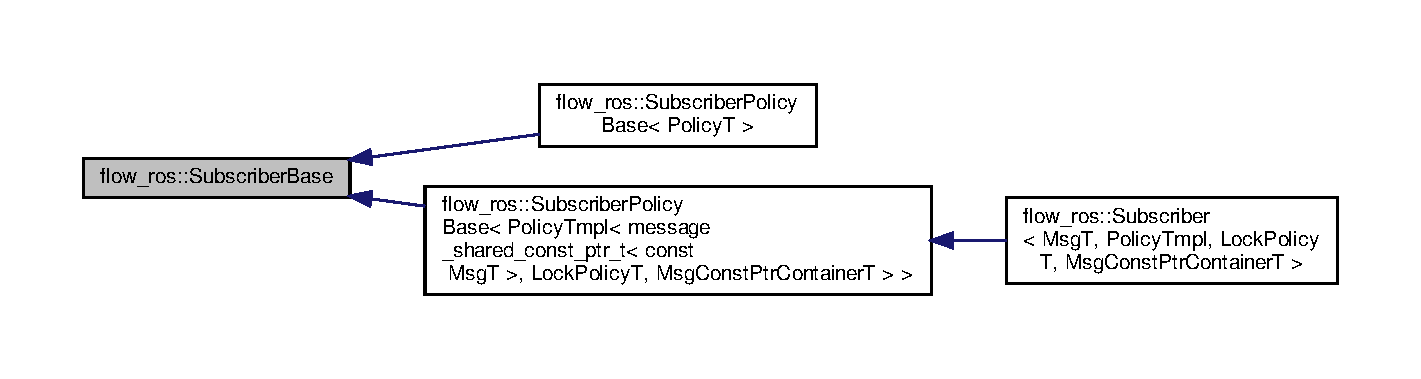
\includegraphics[width=350pt]{classflow__ros_1_1_subscriber_base__inherit__graph}
\end{center}
\end{figure}
\subsection*{Public Member Functions}
\begin{DoxyCompactItemize}
\item 
std\+::string \hyperlink{classflow__ros_1_1_subscriber_base_a3af4148c9a1fef17b9243116260455c7}{get\+Topic} () const
\begin{DoxyCompactList}\small\item\em Returns topic associated with publication. \end{DoxyCompactList}\item 
std\+::uint32\+\_\+t \hyperlink{classflow__ros_1_1_subscriber_base_aabaa5a35708ea005c95b2ab206bc172e}{get\+Num\+Publishers} () const
\begin{DoxyCompactList}\small\item\em Returns number of local publications connected to this subscription. \end{DoxyCompactList}\item 
\hyperlink{transport__info_8h_ae57afcf849a5bdb82b958347c6ccc57b}{routing\+::\+Transport\+Method} \hyperlink{classflow__ros_1_1_subscriber_base_ae68b6a76c0ffc8d2fd8080206f7ce891}{get\+Transport\+Method} () const
\begin{DoxyCompactList}\small\item\em Returns transport method (code) associated with this subscription. \end{DoxyCompactList}\item 
\mbox{\Hypertarget{classflow__ros_1_1_subscriber_base_a25536a5f4b8a3c3dba3b581647e161b5}\label{classflow__ros_1_1_subscriber_base_a25536a5f4b8a3c3dba3b581647e161b5}} 
virtual std\+::size\+\_\+t \hyperlink{classflow__ros_1_1_subscriber_base_a25536a5f4b8a3c3dba3b581647e161b5}{get\+Capacity} () const =0
\begin{DoxyCompactList}\small\item\em Returns underlying {\ttfamily flow\+::\+Captor} buffer capacity. \end{DoxyCompactList}\item 
\mbox{\Hypertarget{classflow__ros_1_1_subscriber_base_a65fa9835d2c8135a5b118279e5cf1588}\label{classflow__ros_1_1_subscriber_base_a65fa9835d2c8135a5b118279e5cf1588}} 
virtual std\+::size\+\_\+t \hyperlink{classflow__ros_1_1_subscriber_base_a65fa9835d2c8135a5b118279e5cf1588}{get\+Num\+Buffered} () const =0
\begin{DoxyCompactList}\small\item\em Returns number of buffers messages in underlying {\ttfamily flow\+::\+Captor} buffer. \end{DoxyCompactList}\item 
\mbox{\Hypertarget{classflow__ros_1_1_subscriber_base_a7cea45e8cbbeb3f7406dd5b4336d86d5}\label{classflow__ros_1_1_subscriber_base_a7cea45e8cbbeb3f7406dd5b4336d86d5}} 
virtual flow\+::\+Capture\+Range$<$ ros\+::\+Time $>$ \hyperlink{classflow__ros_1_1_subscriber_base_a7cea45e8cbbeb3f7406dd5b4336d86d5}{get\+Available\+Buffered\+Range} () const =0
\begin{DoxyCompactList}\small\item\em Returns stamp range of all buffered messages. \end{DoxyCompactList}\item 
bool \hyperlink{classflow__ros_1_1_subscriber_base_a1c2ed330f95a5711c6f71b80b556e742}{is\+Valid} () const
\begin{DoxyCompactList}\small\item\em Validity check. \end{DoxyCompactList}\item 
\mbox{\Hypertarget{classflow__ros_1_1_subscriber_base_a776d32808c392411b4e9b308c79d866b}\label{classflow__ros_1_1_subscriber_base_a776d32808c392411b4e9b308c79d866b}} 
std\+::shared\+\_\+ptr$<$ \hyperlink{classflow__ros_1_1routing_1_1_subscription_wrapper}{routing\+::\+Subscription\+Wrapper} $>$ \hyperlink{classflow__ros_1_1_subscriber_base_a776d32808c392411b4e9b308c79d866b}{impl} () const
\begin{DoxyCompactList}\small\item\em Returns underlying subscription implementation wrapper resource. \end{DoxyCompactList}\end{DoxyCompactItemize}
\subsection*{Static Public Member Functions}
\begin{DoxyCompactItemize}
\item 
static constexpr \hyperlink{transport__info_8h_acb4b6ac875de32a0d0ee8cec235f7752}{routing\+::\+Direction} \hyperlink{classflow__ros_1_1_subscriber_base_a260255c9a1a05e1fa60a076177609f57}{get\+Transport\+Direction} ()
\begin{DoxyCompactList}\small\item\em Returns transport direction (code) associated with this subscription. \end{DoxyCompactList}\end{DoxyCompactItemize}
\subsection*{Protected Attributes}
\begin{DoxyCompactItemize}
\item 
\mbox{\Hypertarget{classflow__ros_1_1_subscriber_base_ac30d4bd880dd826f4930b3abef1da02f}\label{classflow__ros_1_1_subscriber_base_ac30d4bd880dd826f4930b3abef1da02f}} 
std\+::shared\+\_\+ptr$<$ \hyperlink{classflow__ros_1_1routing_1_1_subscription_wrapper}{routing\+::\+Subscription\+Wrapper} $>$ \hyperlink{classflow__ros_1_1_subscriber_base_ac30d4bd880dd826f4930b3abef1da02f}{subscription\+\_\+}
\begin{DoxyCompactList}\small\item\em Underling subscription wrapper. \end{DoxyCompactList}\end{DoxyCompactItemize}


\subsection{Detailed Description}
Message input channel with meta information interfaces. 

\subsection{Member Function Documentation}
\mbox{\Hypertarget{classflow__ros_1_1_subscriber_base_aabaa5a35708ea005c95b2ab206bc172e}\label{classflow__ros_1_1_subscriber_base_aabaa5a35708ea005c95b2ab206bc172e}} 
\index{flow\+\_\+ros\+::\+Subscriber\+Base@{flow\+\_\+ros\+::\+Subscriber\+Base}!get\+Num\+Publishers@{get\+Num\+Publishers}}
\index{get\+Num\+Publishers@{get\+Num\+Publishers}!flow\+\_\+ros\+::\+Subscriber\+Base@{flow\+\_\+ros\+::\+Subscriber\+Base}}
\subsubsection{\texorpdfstring{get\+Num\+Publishers()}{getNumPublishers()}}
{\footnotesize\ttfamily std\+::uint32\+\_\+t flow\+\_\+ros\+::\+Subscriber\+Base\+::get\+Num\+Publishers (\begin{DoxyParamCaption}{ }\end{DoxyParamCaption}) const\hspace{0.3cm}{\ttfamily [inline]}}



Returns number of local publications connected to this subscription. 

\mbox{\Hypertarget{classflow__ros_1_1_subscriber_base_a3af4148c9a1fef17b9243116260455c7}\label{classflow__ros_1_1_subscriber_base_a3af4148c9a1fef17b9243116260455c7}} 
\index{flow\+\_\+ros\+::\+Subscriber\+Base@{flow\+\_\+ros\+::\+Subscriber\+Base}!get\+Topic@{get\+Topic}}
\index{get\+Topic@{get\+Topic}!flow\+\_\+ros\+::\+Subscriber\+Base@{flow\+\_\+ros\+::\+Subscriber\+Base}}
\subsubsection{\texorpdfstring{get\+Topic()}{getTopic()}}
{\footnotesize\ttfamily std\+::string flow\+\_\+ros\+::\+Subscriber\+Base\+::get\+Topic (\begin{DoxyParamCaption}{ }\end{DoxyParamCaption}) const\hspace{0.3cm}{\ttfamily [inline]}}



Returns topic associated with publication. 

\mbox{\Hypertarget{classflow__ros_1_1_subscriber_base_a260255c9a1a05e1fa60a076177609f57}\label{classflow__ros_1_1_subscriber_base_a260255c9a1a05e1fa60a076177609f57}} 
\index{flow\+\_\+ros\+::\+Subscriber\+Base@{flow\+\_\+ros\+::\+Subscriber\+Base}!get\+Transport\+Direction@{get\+Transport\+Direction}}
\index{get\+Transport\+Direction@{get\+Transport\+Direction}!flow\+\_\+ros\+::\+Subscriber\+Base@{flow\+\_\+ros\+::\+Subscriber\+Base}}
\subsubsection{\texorpdfstring{get\+Transport\+Direction()}{getTransportDirection()}}
{\footnotesize\ttfamily static constexpr \hyperlink{transport__info_8h_acb4b6ac875de32a0d0ee8cec235f7752}{routing\+::\+Direction} flow\+\_\+ros\+::\+Subscriber\+Base\+::get\+Transport\+Direction (\begin{DoxyParamCaption}{ }\end{DoxyParamCaption})\hspace{0.3cm}{\ttfamily [inline]}, {\ttfamily [static]}}



Returns transport direction (code) associated with this subscription. 

\mbox{\Hypertarget{classflow__ros_1_1_subscriber_base_ae68b6a76c0ffc8d2fd8080206f7ce891}\label{classflow__ros_1_1_subscriber_base_ae68b6a76c0ffc8d2fd8080206f7ce891}} 
\index{flow\+\_\+ros\+::\+Subscriber\+Base@{flow\+\_\+ros\+::\+Subscriber\+Base}!get\+Transport\+Method@{get\+Transport\+Method}}
\index{get\+Transport\+Method@{get\+Transport\+Method}!flow\+\_\+ros\+::\+Subscriber\+Base@{flow\+\_\+ros\+::\+Subscriber\+Base}}
\subsubsection{\texorpdfstring{get\+Transport\+Method()}{getTransportMethod()}}
{\footnotesize\ttfamily \hyperlink{transport__info_8h_ae57afcf849a5bdb82b958347c6ccc57b}{routing\+::\+Transport\+Method} flow\+\_\+ros\+::\+Subscriber\+Base\+::get\+Transport\+Method (\begin{DoxyParamCaption}{ }\end{DoxyParamCaption}) const\hspace{0.3cm}{\ttfamily [inline]}}



Returns transport method (code) associated with this subscription. 

\mbox{\Hypertarget{classflow__ros_1_1_subscriber_base_a1c2ed330f95a5711c6f71b80b556e742}\label{classflow__ros_1_1_subscriber_base_a1c2ed330f95a5711c6f71b80b556e742}} 
\index{flow\+\_\+ros\+::\+Subscriber\+Base@{flow\+\_\+ros\+::\+Subscriber\+Base}!is\+Valid@{is\+Valid}}
\index{is\+Valid@{is\+Valid}!flow\+\_\+ros\+::\+Subscriber\+Base@{flow\+\_\+ros\+::\+Subscriber\+Base}}
\subsubsection{\texorpdfstring{is\+Valid()}{isValid()}}
{\footnotesize\ttfamily bool flow\+\_\+ros\+::\+Subscriber\+Base\+::is\+Valid (\begin{DoxyParamCaption}{ }\end{DoxyParamCaption}) const\hspace{0.3cm}{\ttfamily [inline]}}



Validity check. 



The documentation for this class was generated from the following file\+:\begin{DoxyCompactItemize}
\item 
flow\+\_\+ros/include/\hyperlink{subscriber_8h}{subscriber.\+h}\end{DoxyCompactItemize}

\hypertarget{classflow__ros_1_1_subscriber_policy_base}{}\section{flow\+\_\+ros\+:\+:Subscriber\+Policy\+Base$<$ PolicyT $>$ Class Template Reference}
\label{classflow__ros_1_1_subscriber_policy_base}\index{flow\+\_\+ros\+::\+Subscriber\+Policy\+Base$<$ Policy\+T $>$@{flow\+\_\+ros\+::\+Subscriber\+Policy\+Base$<$ Policy\+T $>$}}


Message input channel with an associated capture policy.  




{\ttfamily \#include $<$subscriber.\+h$>$}



Inheritance diagram for flow\+\_\+ros\+:\+:Subscriber\+Policy\+Base$<$ PolicyT $>$\+:\nopagebreak
\begin{figure}[H]
\begin{center}
\leavevmode
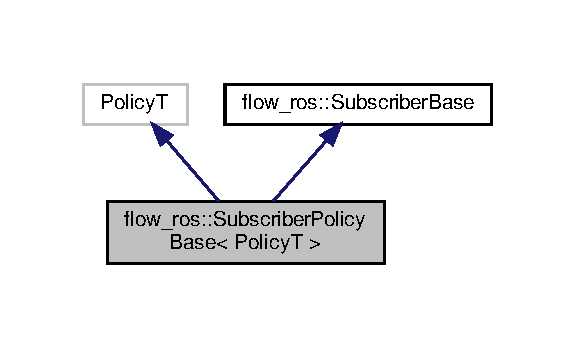
\includegraphics[width=276pt]{classflow__ros_1_1_subscriber_policy_base__inherit__graph}
\end{center}
\end{figure}


Collaboration diagram for flow\+\_\+ros\+:\+:Subscriber\+Policy\+Base$<$ PolicyT $>$\+:\nopagebreak
\begin{figure}[H]
\begin{center}
\leavevmode
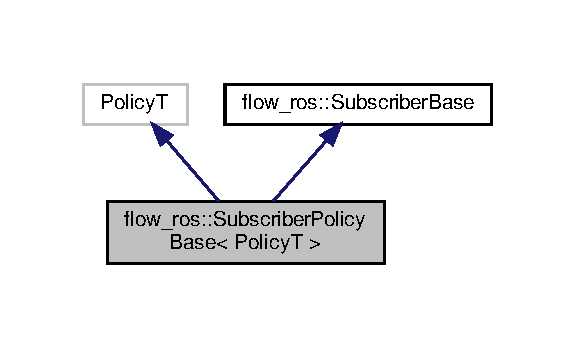
\includegraphics[width=276pt]{classflow__ros_1_1_subscriber_policy_base__coll__graph}
\end{center}
\end{figure}
\subsection*{Public Member Functions}
\begin{DoxyCompactItemize}
\item 
std\+::size\+\_\+t \hyperlink{classflow__ros_1_1_subscriber_policy_base_ad386c7963771122c13674afc5934c371}{get\+Capacity} () const final
\begin{DoxyCompactList}\small\item\em Check that PolicyT is a flow\+::\+Captor derivative. \end{DoxyCompactList}\item 
\mbox{\Hypertarget{classflow__ros_1_1_subscriber_policy_base_a2c99605a1aef9b82087bc0f74b267ecc}\label{classflow__ros_1_1_subscriber_policy_base_a2c99605a1aef9b82087bc0f74b267ecc}} 
std\+::size\+\_\+t \hyperlink{classflow__ros_1_1_subscriber_policy_base_a2c99605a1aef9b82087bc0f74b267ecc}{get\+Num\+Buffered} () const final
\begin{DoxyCompactList}\small\item\em Returns number of buffers messages in underlying {\ttfamily flow\+::\+Captor} buffer. \end{DoxyCompactList}\item 
\mbox{\Hypertarget{classflow__ros_1_1_subscriber_policy_base_a5e6741fd671b011356b1374d500cbd38}\label{classflow__ros_1_1_subscriber_policy_base_a5e6741fd671b011356b1374d500cbd38}} 
flow\+::\+Capture\+Range$<$ ros\+::\+Time $>$ \hyperlink{classflow__ros_1_1_subscriber_policy_base_a5e6741fd671b011356b1374d500cbd38}{get\+Available\+Buffered\+Range} () const final
\begin{DoxyCompactList}\small\item\em Returns stamp range of all buffered messages. \end{DoxyCompactList}\end{DoxyCompactItemize}
\subsection*{Protected Member Functions}
\begin{DoxyCompactItemize}
\item 
\mbox{\Hypertarget{classflow__ros_1_1_subscriber_policy_base_ad74822efa225007b31fb6ea4b34898d0}\label{classflow__ros_1_1_subscriber_policy_base_ad74822efa225007b31fb6ea4b34898d0}} 
{\footnotesize template$<$typename... Policy\+Arg\+Ts$>$ }\\\hyperlink{classflow__ros_1_1_subscriber_policy_base_ad74822efa225007b31fb6ea4b34898d0}{Subscriber\+Policy\+Base} (Policy\+Arg\+Ts \&\&... policy\+\_\+args)
\begin{DoxyCompactList}\small\item\em Policy setup constructor. \end{DoxyCompactList}\end{DoxyCompactItemize}
\subsection*{Additional Inherited Members}


\subsection{Detailed Description}
\subsubsection*{template$<$typename PolicyT$>$\newline
class flow\+\_\+ros\+::\+Subscriber\+Policy\+Base$<$ Policy\+T $>$}

Message input channel with an associated capture policy. 


\begin{DoxyTemplParams}{Template Parameters}
{\em PolicyT} & underlying Captor type with synchronization policy \\
\hline
\end{DoxyTemplParams}


\subsection{Member Function Documentation}
\mbox{\Hypertarget{classflow__ros_1_1_subscriber_policy_base_ad386c7963771122c13674afc5934c371}\label{classflow__ros_1_1_subscriber_policy_base_ad386c7963771122c13674afc5934c371}} 
\index{flow\+\_\+ros\+::\+Subscriber\+Policy\+Base@{flow\+\_\+ros\+::\+Subscriber\+Policy\+Base}!get\+Capacity@{get\+Capacity}}
\index{get\+Capacity@{get\+Capacity}!flow\+\_\+ros\+::\+Subscriber\+Policy\+Base@{flow\+\_\+ros\+::\+Subscriber\+Policy\+Base}}
\subsubsection{\texorpdfstring{get\+Capacity()}{getCapacity()}}
{\footnotesize\ttfamily template$<$typename PolicyT$>$ \\
std\+::size\+\_\+t \hyperlink{classflow__ros_1_1_subscriber_policy_base}{flow\+\_\+ros\+::\+Subscriber\+Policy\+Base}$<$ PolicyT $>$\+::get\+Capacity (\begin{DoxyParamCaption}{ }\end{DoxyParamCaption}) const\hspace{0.3cm}{\ttfamily [inline]}, {\ttfamily [final]}, {\ttfamily [virtual]}}



Check that PolicyT is a flow\+::\+Captor derivative. 

Returns underlying {\ttfamily flow\+::\+Captor} buffer capacity 

Implements \hyperlink{classflow__ros_1_1_subscriber_base_a25536a5f4b8a3c3dba3b581647e161b5}{flow\+\_\+ros\+::\+Subscriber\+Base}.



The documentation for this class was generated from the following file\+:\begin{DoxyCompactItemize}
\item 
flow\+\_\+ros/include/\hyperlink{subscriber_8h}{subscriber.\+h}\end{DoxyCompactItemize}

\hypertarget{structflow__ros_1_1_subscriber_traits}{}\section{flow\+\_\+ros\+:\+:Subscriber\+Traits$<$ MsgT $>$ Struct Template Reference}
\label{structflow__ros_1_1_subscriber_traits}\index{flow\+\_\+ros\+::\+Subscriber\+Traits$<$ Msg\+T $>$@{flow\+\_\+ros\+::\+Subscriber\+Traits$<$ Msg\+T $>$}}


\hyperlink{classflow__ros_1_1_subscriber}{Subscriber} type traits.  




{\ttfamily \#include $<$subscriber.\+h$>$}



\subsection{Detailed Description}
\subsubsection*{template$<$typename MsgT$>$\newline
struct flow\+\_\+ros\+::\+Subscriber\+Traits$<$ Msg\+T $>$}

\hyperlink{classflow__ros_1_1_subscriber}{Subscriber} type traits. 

The documentation for this struct was generated from the following file\+:\begin{DoxyCompactItemize}
\item 
flow\+\_\+ros/include/\hyperlink{subscriber_8h}{subscriber.\+h}\end{DoxyCompactItemize}

\hypertarget{structflow__ros_1_1_subscriber_traits_3_01_subscriber_3_01_msg_t_00_01_policy_tmpl_00_01_lock_policy_t_01_4_01_4}{}\section{flow\+\_\+ros\+:\+:Subscriber\+Traits$<$ Subscriber$<$ MsgT, Policy\+Tmpl, Lock\+PolicyT $>$ $>$ Struct Template Reference}
\label{structflow__ros_1_1_subscriber_traits_3_01_subscriber_3_01_msg_t_00_01_policy_tmpl_00_01_lock_policy_t_01_4_01_4}\index{flow\+\_\+ros\+::\+Subscriber\+Traits$<$ Subscriber$<$ Msg\+T, Policy\+Tmpl, Lock\+Policy\+T $>$ $>$@{flow\+\_\+ros\+::\+Subscriber\+Traits$<$ Subscriber$<$ Msg\+T, Policy\+Tmpl, Lock\+Policy\+T $>$ $>$}}


\hyperlink{classflow__ros_1_1_subscriber}{Subscriber} type traits.  




{\ttfamily \#include $<$subscriber.\+h$>$}

\subsection*{Public Types}
\begin{DoxyCompactItemize}
\item 
\mbox{\Hypertarget{structflow__ros_1_1_subscriber_traits_3_01_subscriber_3_01_msg_t_00_01_policy_tmpl_00_01_lock_policy_t_01_4_01_4_adab0c086537ed432b04633406513c28a}\label{structflow__ros_1_1_subscriber_traits_3_01_subscriber_3_01_msg_t_00_01_policy_tmpl_00_01_lock_policy_t_01_4_01_4_adab0c086537ed432b04633406513c28a}} 
using \hyperlink{structflow__ros_1_1_subscriber_traits_3_01_subscriber_3_01_msg_t_00_01_policy_tmpl_00_01_lock_policy_t_01_4_01_4_adab0c086537ed432b04633406513c28a}{Msg\+Type} = MsgT
\begin{DoxyCompactList}\small\item\em Input message type. \end{DoxyCompactList}\item 
\mbox{\Hypertarget{structflow__ros_1_1_subscriber_traits_3_01_subscriber_3_01_msg_t_00_01_policy_tmpl_00_01_lock_policy_t_01_4_01_4_aa431ca3ab1e84d5ee2c8e956635b1587}\label{structflow__ros_1_1_subscriber_traits_3_01_subscriber_3_01_msg_t_00_01_policy_tmpl_00_01_lock_policy_t_01_4_01_4_aa431ca3ab1e84d5ee2c8e956635b1587}} 
using \hyperlink{structflow__ros_1_1_subscriber_traits_3_01_subscriber_3_01_msg_t_00_01_policy_tmpl_00_01_lock_policy_t_01_4_01_4_aa431ca3ab1e84d5ee2c8e956635b1587}{Policy\+Type} = Policy\+Tmpl$<$ \hyperlink{namespaceflow__ros_ad222b6c2bd0341c551129c3a03241ad7}{message\+\_\+shared\+\_\+const\+\_\+ptr\+\_\+t}$<$ MsgT $>$, Lock\+PolicyT $>$
\begin{DoxyCompactList}\small\item\em Base capture policy type. \end{DoxyCompactList}\end{DoxyCompactItemize}


\subsection{Detailed Description}
\subsubsection*{template$<$typename MsgT, template$<$ typename... $>$ class Policy\+Tmpl, typename Lock\+PolicyT$>$\newline
struct flow\+\_\+ros\+::\+Subscriber\+Traits$<$ Subscriber$<$ Msg\+T, Policy\+Tmpl, Lock\+Policy\+T $>$ $>$}

\hyperlink{classflow__ros_1_1_subscriber}{Subscriber} type traits. 

\begin{DoxyNote}{Note}
\hyperlink{classflow__ros_1_1_subscriber}{Subscriber} partial specialization 
\end{DoxyNote}


The documentation for this struct was generated from the following file\+:\begin{DoxyCompactItemize}
\item 
flow\+\_\+ros/include/\hyperlink{subscriber_8h}{subscriber.\+h}\end{DoxyCompactItemize}

\hypertarget{classflow__ros_1_1routing_1_1_subscription_wrapper}{}\section{flow\+\_\+ros\+:\+:routing\+:\+:Subscription\+Wrapper Class Reference}
\label{classflow__ros_1_1routing_1_1_subscription_wrapper}\index{flow\+\_\+ros\+::routing\+::\+Subscription\+Wrapper@{flow\+\_\+ros\+::routing\+::\+Subscription\+Wrapper}}


Base for message subscribing implementation.  




{\ttfamily \#include $<$subscription\+\_\+wrapper.\+h$>$}



Inheritance diagram for flow\+\_\+ros\+:\+:routing\+:\+:Subscription\+Wrapper\+:\nopagebreak
\begin{figure}[H]
\begin{center}
\leavevmode
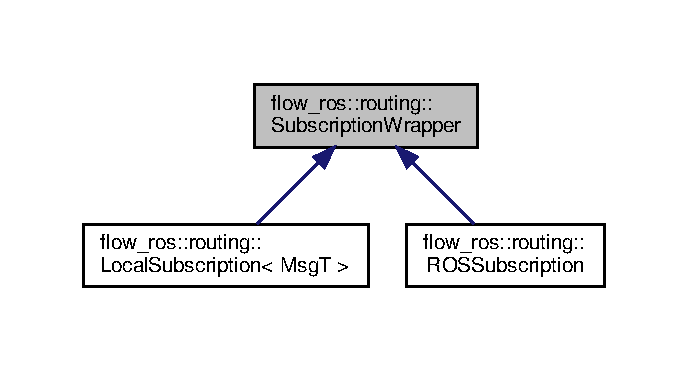
\includegraphics[width=330pt]{classflow__ros_1_1routing_1_1_subscription_wrapper__inherit__graph}
\end{center}
\end{figure}
\subsection*{Public Member Functions}
\begin{DoxyCompactItemize}
\item 
\mbox{\Hypertarget{classflow__ros_1_1routing_1_1_subscription_wrapper_a2ef27475e7b7d7555e90d02cdc220b88}\label{classflow__ros_1_1routing_1_1_subscription_wrapper_a2ef27475e7b7d7555e90d02cdc220b88}} 
virtual std\+::string \hyperlink{classflow__ros_1_1routing_1_1_subscription_wrapper_a2ef27475e7b7d7555e90d02cdc220b88}{get\+Topic} () const =0
\begin{DoxyCompactList}\small\item\em Returns topic associated with publication. \end{DoxyCompactList}\item 
\mbox{\Hypertarget{classflow__ros_1_1routing_1_1_subscription_wrapper_a8ae55d34a07c505dc2b4bcb2440b2d32}\label{classflow__ros_1_1routing_1_1_subscription_wrapper_a8ae55d34a07c505dc2b4bcb2440b2d32}} 
virtual std\+::uint32\+\_\+t \hyperlink{classflow__ros_1_1routing_1_1_subscription_wrapper_a8ae55d34a07c505dc2b4bcb2440b2d32}{get\+Num\+Publishers} () const =0
\begin{DoxyCompactList}\small\item\em Returns number of local publications connected to this subscription. \end{DoxyCompactList}\item 
\mbox{\Hypertarget{classflow__ros_1_1routing_1_1_subscription_wrapper_a063fcc10600ef657620e2b58ce1fca85}\label{classflow__ros_1_1routing_1_1_subscription_wrapper_a063fcc10600ef657620e2b58ce1fca85}} 
virtual \hyperlink{transport__info_8h_ae57afcf849a5bdb82b958347c6ccc57b}{Transport\+Method} \hyperlink{classflow__ros_1_1routing_1_1_subscription_wrapper_a063fcc10600ef657620e2b58ce1fca85}{get\+Transport\+Method} () const =0
\begin{DoxyCompactList}\small\item\em Returns transport method (code) associated with this subscription. \end{DoxyCompactList}\item 
\mbox{\Hypertarget{classflow__ros_1_1routing_1_1_subscription_wrapper_a0f23052807c3533d28168d7c681a221e}\label{classflow__ros_1_1routing_1_1_subscription_wrapper_a0f23052807c3533d28168d7c681a221e}} 
virtual bool \hyperlink{classflow__ros_1_1routing_1_1_subscription_wrapper_a0f23052807c3533d28168d7c681a221e}{is\+Valid} () const =0
\begin{DoxyCompactList}\small\item\em Validity check. \end{DoxyCompactList}\item 
\mbox{\Hypertarget{classflow__ros_1_1routing_1_1_subscription_wrapper_a6869138ff591ba2ea7b2c81f2ad0ef89}\label{classflow__ros_1_1routing_1_1_subscription_wrapper_a6869138ff591ba2ea7b2c81f2ad0ef89}} 
virtual \hyperlink{classflow__ros_1_1routing_1_1_subscription_wrapper_a6869138ff591ba2ea7b2c81f2ad0ef89}{operator bool} () const
\begin{DoxyCompactList}\small\item\em Validity check cast. \end{DoxyCompactList}\end{DoxyCompactItemize}
\subsection*{Static Public Member Functions}
\begin{DoxyCompactItemize}
\item 
\mbox{\Hypertarget{classflow__ros_1_1routing_1_1_subscription_wrapper_a1a5c5359666278e172d50a8dde94b77f}\label{classflow__ros_1_1routing_1_1_subscription_wrapper_a1a5c5359666278e172d50a8dde94b77f}} 
static constexpr \hyperlink{transport__info_8h_acb4b6ac875de32a0d0ee8cec235f7752}{Direction} \hyperlink{classflow__ros_1_1routing_1_1_subscription_wrapper_a1a5c5359666278e172d50a8dde94b77f}{get\+Transport\+Direction} ()
\begin{DoxyCompactList}\small\item\em Returns transport direction (code) associated with this subscription. \end{DoxyCompactList}\end{DoxyCompactItemize}


\subsection{Detailed Description}
Base for message subscribing implementation. 

The documentation for this class was generated from the following file\+:\begin{DoxyCompactItemize}
\item 
flow\+\_\+ros/include/routing/\hyperlink{subscription__wrapper_8h}{subscription\+\_\+wrapper.\+h}\end{DoxyCompactItemize}

\hypertarget{struct_test_message}{}\section{Test\+Message Struct Reference}
\label{struct_test_message}\index{Test\+Message@{Test\+Message}}


A R\+OS messages-\/like object.  


\subsection*{Public Types}
\begin{DoxyCompactItemize}
\item 
\mbox{\Hypertarget{struct_test_message_a61078aaa4d453510b1a9768f39b779b8}\label{struct_test_message_a61078aaa4d453510b1a9768f39b779b8}} 
using {\bfseries Ptr} = std\+::shared\+\_\+ptr$<$ \hyperlink{struct_test_message}{Test\+Message} $>$
\item 
\mbox{\Hypertarget{struct_test_message_aacafaf7937f1d6971e0fd32089695ca8}\label{struct_test_message_aacafaf7937f1d6971e0fd32089695ca8}} 
using {\bfseries Const\+Ptr} = std\+::shared\+\_\+ptr$<$ const \hyperlink{struct_test_message}{Test\+Message} $>$
\item 
\mbox{\Hypertarget{struct_test_message_a61078aaa4d453510b1a9768f39b779b8}\label{struct_test_message_a61078aaa4d453510b1a9768f39b779b8}} 
using {\bfseries Ptr} = std\+::shared\+\_\+ptr$<$ \hyperlink{struct_test_message}{Test\+Message} $>$
\item 
\mbox{\Hypertarget{struct_test_message_aacafaf7937f1d6971e0fd32089695ca8}\label{struct_test_message_aacafaf7937f1d6971e0fd32089695ca8}} 
using {\bfseries Const\+Ptr} = std\+::shared\+\_\+ptr$<$ const \hyperlink{struct_test_message}{Test\+Message} $>$
\item 
\mbox{\Hypertarget{struct_test_message_a61078aaa4d453510b1a9768f39b779b8}\label{struct_test_message_a61078aaa4d453510b1a9768f39b779b8}} 
using {\bfseries Ptr} = std\+::shared\+\_\+ptr$<$ \hyperlink{struct_test_message}{Test\+Message} $>$
\item 
\mbox{\Hypertarget{struct_test_message_aacafaf7937f1d6971e0fd32089695ca8}\label{struct_test_message_aacafaf7937f1d6971e0fd32089695ca8}} 
using {\bfseries Const\+Ptr} = std\+::shared\+\_\+ptr$<$ const \hyperlink{struct_test_message}{Test\+Message} $>$
\end{DoxyCompactItemize}
\subsection*{Public Attributes}
\begin{DoxyCompactItemize}
\item 
\mbox{\Hypertarget{struct_test_message_a3fa194f99a95061a0c390f18be03394e}\label{struct_test_message_a3fa194f99a95061a0c390f18be03394e}} 
std\+\_\+msgs\+::\+Header {\bfseries header}
\end{DoxyCompactItemize}


\subsection{Detailed Description}
A R\+OS messages-\/like object. 

\begin{DoxyCopyright}{Copyright}
2020 Fetch Robotics Inc. 
\end{DoxyCopyright}
\begin{DoxyAuthor}{Author}
Brian Cairl 
\end{DoxyAuthor}


The documentation for this struct was generated from the following files\+:\begin{DoxyCompactItemize}
\item 
flow\+\_\+ros/test/unit/publisher.\+cpp\item 
flow\+\_\+ros/test/unit/router.\+cpp\item 
flow\+\_\+ros/test/unit/subscriber.\+cpp\end{DoxyCompactItemize}

\hypertarget{struct_test_message1}{}\section{Test\+Message1 Struct Reference}
\label{struct_test_message1}\index{Test\+Message1@{Test\+Message1}}


A R\+OS messages-\/like object.  


\subsection*{Public Types}
\begin{DoxyCompactItemize}
\item 
\mbox{\Hypertarget{struct_test_message1_afebf7176422a7ae4fd3c6e505dbd7fcb}\label{struct_test_message1_afebf7176422a7ae4fd3c6e505dbd7fcb}} 
using {\bfseries Ptr} = std\+::shared\+\_\+ptr$<$ \hyperlink{struct_test_message1}{Test\+Message1} $>$
\item 
\mbox{\Hypertarget{struct_test_message1_a12a11018fd576f645ecf2abfff986453}\label{struct_test_message1_a12a11018fd576f645ecf2abfff986453}} 
using {\bfseries Const\+Ptr} = std\+::shared\+\_\+ptr$<$ const \hyperlink{struct_test_message1}{Test\+Message1} $>$
\end{DoxyCompactItemize}
\subsection*{Public Attributes}
\begin{DoxyCompactItemize}
\item 
\mbox{\Hypertarget{struct_test_message1_a77d94be075633cc256e0502cfdd479ca}\label{struct_test_message1_a77d94be075633cc256e0502cfdd479ca}} 
std\+\_\+msgs\+::\+Header {\bfseries header}
\end{DoxyCompactItemize}


\subsection{Detailed Description}
A R\+OS messages-\/like object. 

The documentation for this struct was generated from the following file\+:\begin{DoxyCompactItemize}
\item 
flow\+\_\+ros/test/unit/\hyperlink{event__handler_8cpp}{event\+\_\+handler.\+cpp}\end{DoxyCompactItemize}

\hypertarget{struct_test_message2}{}\section{Test\+Message2 Struct Reference}
\label{struct_test_message2}\index{Test\+Message2@{Test\+Message2}}
\subsection*{Public Types}
\begin{DoxyCompactItemize}
\item 
\mbox{\Hypertarget{struct_test_message2_a864b45356c57ef91655aabe71f249fee}\label{struct_test_message2_a864b45356c57ef91655aabe71f249fee}} 
using {\bfseries Ptr} = std\+::shared\+\_\+ptr$<$ \hyperlink{struct_test_message2}{Test\+Message2} $>$
\item 
\mbox{\Hypertarget{struct_test_message2_a1490b1301121126708856860a6aa2138}\label{struct_test_message2_a1490b1301121126708856860a6aa2138}} 
using {\bfseries Const\+Ptr} = std\+::shared\+\_\+ptr$<$ const \hyperlink{struct_test_message2}{Test\+Message2} $>$
\end{DoxyCompactItemize}
\subsection*{Public Attributes}
\begin{DoxyCompactItemize}
\item 
\mbox{\Hypertarget{struct_test_message2_a97d834fedcb6dbb80f316d2ff3751d8f}\label{struct_test_message2_a97d834fedcb6dbb80f316d2ff3751d8f}} 
std\+\_\+msgs\+::\+Header {\bfseries header}
\end{DoxyCompactItemize}


The documentation for this struct was generated from the following file\+:\begin{DoxyCompactItemize}
\item 
flow\+\_\+ros/test/unit/\hyperlink{event__handler_8cpp}{event\+\_\+handler.\+cpp}\end{DoxyCompactItemize}

\hypertarget{classflow__ros_1_1_unknown_subscription_error}{}\section{flow\+\_\+ros\+:\+:Unknown\+Subscription\+Error Class Reference}
\label{classflow__ros_1_1_unknown_subscription_error}\index{flow\+\_\+ros\+::\+Unknown\+Subscription\+Error@{flow\+\_\+ros\+::\+Unknown\+Subscription\+Error}}


Exception thrown when message for an unknown subscription is injected.  




{\ttfamily \#include $<$router.\+h$>$}



Inheritance diagram for flow\+\_\+ros\+:\+:Unknown\+Subscription\+Error\+:\nopagebreak
\begin{figure}[H]
\begin{center}
\leavevmode
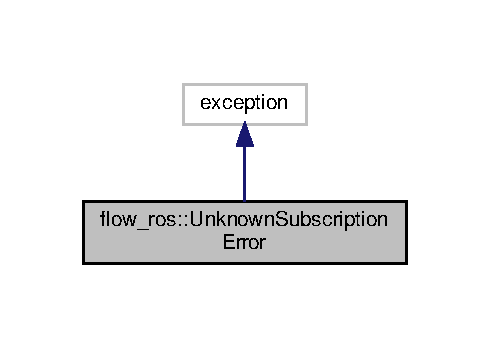
\includegraphics[width=235pt]{classflow__ros_1_1_unknown_subscription_error__inherit__graph}
\end{center}
\end{figure}


Collaboration diagram for flow\+\_\+ros\+:\+:Unknown\+Subscription\+Error\+:\nopagebreak
\begin{figure}[H]
\begin{center}
\leavevmode
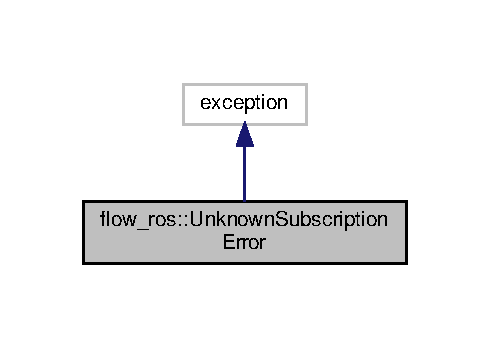
\includegraphics[width=235pt]{classflow__ros_1_1_unknown_subscription_error__coll__graph}
\end{center}
\end{figure}
\subsection*{Public Member Functions}
\begin{DoxyCompactItemize}
\item 
\mbox{\Hypertarget{classflow__ros_1_1_unknown_subscription_error_a7583ea02082517c342cf9634d8d39806}\label{classflow__ros_1_1_unknown_subscription_error_a7583ea02082517c342cf9634d8d39806}} 
{\footnotesize template$<$typename StringT $>$ }\\{\bfseries Unknown\+Subscription\+Error} (StringT \&\&what)
\item 
\mbox{\Hypertarget{classflow__ros_1_1_unknown_subscription_error_a148fedb06eae3261c5634042c4359a7d}\label{classflow__ros_1_1_unknown_subscription_error_a148fedb06eae3261c5634042c4359a7d}} 
const char $\ast$ {\bfseries what} () const noexcept
\end{DoxyCompactItemize}


\subsection{Detailed Description}
Exception thrown when message for an unknown subscription is injected. 

The documentation for this class was generated from the following file\+:\begin{DoxyCompactItemize}
\item 
flow\+\_\+ros/include/\hyperlink{router_8h}{router.\+h}\end{DoxyCompactItemize}

\hypertarget{structflow__ros_1_1detail_1_1_wrap_tuple_elements}{}\section{flow\+\_\+ros\+:\+:detail\+:\+:Wrap\+Tuple\+Elements$<$ Wrapper\+Tmpl, Channel\+Type $>$ Struct Template Reference}
\label{structflow__ros_1_1detail_1_1_wrap_tuple_elements}\index{flow\+\_\+ros\+::detail\+::\+Wrap\+Tuple\+Elements$<$ Wrapper\+Tmpl, Channel\+Type $>$@{flow\+\_\+ros\+::detail\+::\+Wrap\+Tuple\+Elements$<$ Wrapper\+Tmpl, Channel\+Type $>$}}


Wraps tuple element types in with template to generate a new tuple type.  




{\ttfamily \#include $<$event\+\_\+handler.\+hpp$>$}

\subsection*{Public Types}
\begin{DoxyCompactItemize}
\item 
\mbox{\Hypertarget{structflow__ros_1_1detail_1_1_wrap_tuple_elements_a1e7175caae34df8828f5ff605fa4cae2}\label{structflow__ros_1_1detail_1_1_wrap_tuple_elements_a1e7175caae34df8828f5ff605fa4cae2}} 
using {\bfseries type} = std\+::tuple$<$ Wrapper\+Tmpl$<$ Channel\+Type $>$ $>$
\end{DoxyCompactItemize}


\subsection{Detailed Description}
\subsubsection*{template$<$template$<$ typename... $>$ class Wrapper\+Tmpl, typename Channel\+Type$>$\newline
struct flow\+\_\+ros\+::detail\+::\+Wrap\+Tuple\+Elements$<$ Wrapper\+Tmpl, Channel\+Type $>$}

Wraps tuple element types in with template to generate a new tuple type. 

The documentation for this struct was generated from the following file\+:\begin{DoxyCompactItemize}
\item 
flow\+\_\+ros/include/impl/event\+\_\+handler.\+hpp\end{DoxyCompactItemize}

\hypertarget{structflow__ros_1_1detail_1_1_wrap_tuple_elements_3_01_wrapper_tmpl_00_01std_1_1tuple_3_01_channel_ts_8_8_8_01_4_01_4}{}\section{flow\+\_\+ros\+:\+:detail\+:\+:Wrap\+Tuple\+Elements$<$ Wrapper\+Tmpl, std\+:\+:tuple$<$ Channel\+Ts... $>$ $>$ Struct Template Reference}
\label{structflow__ros_1_1detail_1_1_wrap_tuple_elements_3_01_wrapper_tmpl_00_01std_1_1tuple_3_01_channel_ts_8_8_8_01_4_01_4}\index{flow\+\_\+ros\+::detail\+::\+Wrap\+Tuple\+Elements$<$ Wrapper\+Tmpl, std\+::tuple$<$ Channel\+Ts... $>$ $>$@{flow\+\_\+ros\+::detail\+::\+Wrap\+Tuple\+Elements$<$ Wrapper\+Tmpl, std\+::tuple$<$ Channel\+Ts... $>$ $>$}}


Wraps tuple element types in with template to generate a new tuple type.  




{\ttfamily \#include $<$event\+\_\+handler.\+hpp$>$}

\subsection*{Public Types}
\begin{DoxyCompactItemize}
\item 
\mbox{\Hypertarget{structflow__ros_1_1detail_1_1_wrap_tuple_elements_3_01_wrapper_tmpl_00_01std_1_1tuple_3_01_channel_ts_8_8_8_01_4_01_4_a8b43c21ef0ca93eef58f776f944eb100}\label{structflow__ros_1_1detail_1_1_wrap_tuple_elements_3_01_wrapper_tmpl_00_01std_1_1tuple_3_01_channel_ts_8_8_8_01_4_01_4_a8b43c21ef0ca93eef58f776f944eb100}} 
using {\bfseries type} = std\+::tuple$<$ Wrapper\+Tmpl$<$ Channel\+Ts $>$... $>$
\end{DoxyCompactItemize}


\subsection{Detailed Description}
\subsubsection*{template$<$template$<$ typename... $>$ class Wrapper\+Tmpl, typename... Channel\+Ts$>$\newline
struct flow\+\_\+ros\+::detail\+::\+Wrap\+Tuple\+Elements$<$ Wrapper\+Tmpl, std\+::tuple$<$ Channel\+Ts... $>$ $>$}

Wraps tuple element types in with template to generate a new tuple type. 

\begin{DoxyNote}{Note}
Multi-\/element specialization 
\end{DoxyNote}


The documentation for this struct was generated from the following file\+:\begin{DoxyCompactItemize}
\item 
flow\+\_\+ros/include/impl/event\+\_\+handler.\+hpp\end{DoxyCompactItemize}

\chapter{File Documentation}
\hypertarget{event__handler_8h}{}\section{flow\+\_\+ros/include/event\+\_\+handler.h File Reference}
\label{event__handler_8h}\index{flow\+\_\+ros/include/event\+\_\+handler.\+h@{flow\+\_\+ros/include/event\+\_\+handler.\+h}}
{\ttfamily \#include $<$chrono$>$}\newline
{\ttfamily \#include $<$functional$>$}\newline
{\ttfamily \#include $<$iterator$>$}\newline
{\ttfamily \#include $<$memory$>$}\newline
{\ttfamily \#include $<$stdexcept$>$}\newline
{\ttfamily \#include $<$tuple$>$}\newline
{\ttfamily \#include $<$utility$>$}\newline
{\ttfamily \#include $<$vector$>$}\newline
{\ttfamily \#include $<$flow/synchronizer.\+h$>$}\newline
{\ttfamily \#include $<$flow\+\_\+ros/message\+\_\+stamp\+\_\+access.\+h$>$}\newline
{\ttfamily \#include $<$flow\+\_\+ros/publisher.\+h$>$}\newline
{\ttfamily \#include $<$flow\+\_\+ros/subscriber.\+h$>$}\newline
{\ttfamily \#include $<$flow\+\_\+ros/impl/event\+\_\+handler.\+hpp$>$}\newline
Include dependency graph for event\+\_\+handler.\+h\+:\nopagebreak
\begin{figure}[H]
\begin{center}
\leavevmode
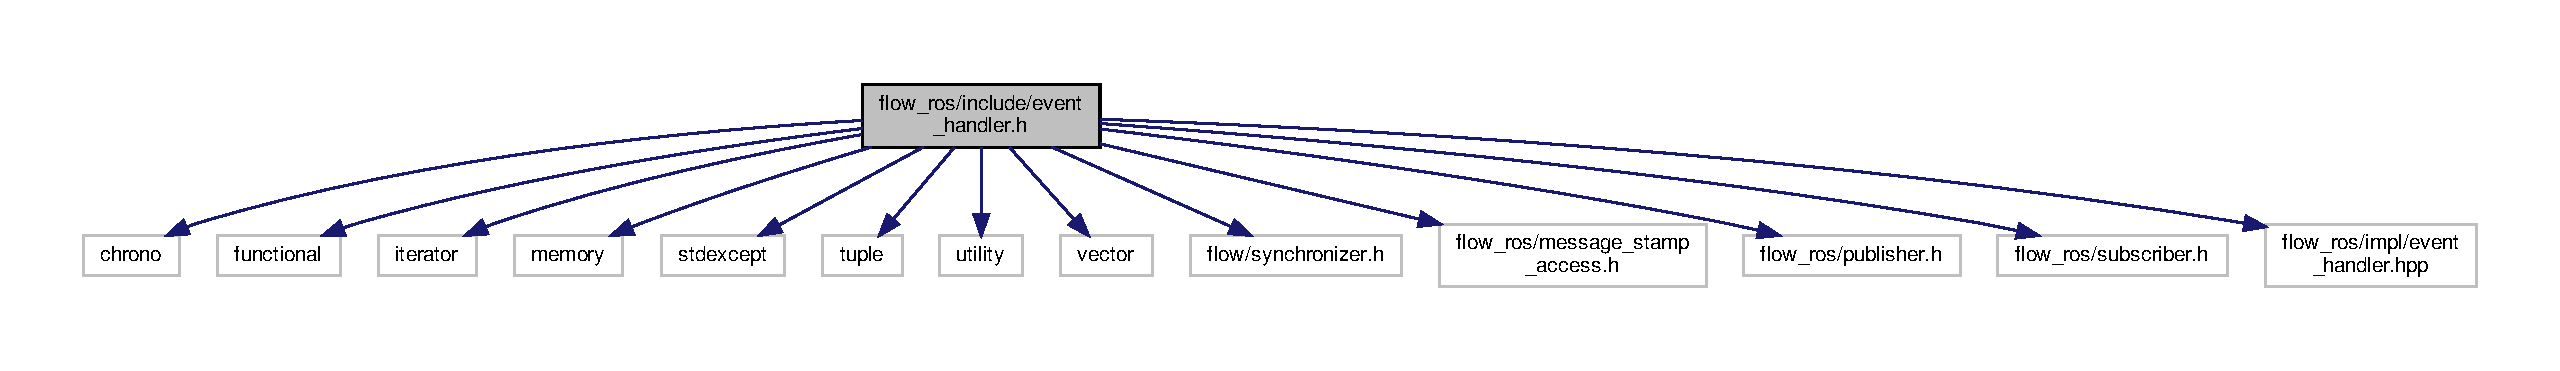
\includegraphics[width=350pt]{event__handler_8h__incl}
\end{center}
\end{figure}
\subsection*{Classes}
\begin{DoxyCompactItemize}
\item 
struct \hyperlink{structflow__ros_1_1_event_summary}{flow\+\_\+ros\+::\+Event\+Summary}
\begin{DoxyCompactList}\small\item\em Summary of event information from results. \end{DoxyCompactList}\item 
class \hyperlink{classflow__ros_1_1_event_handler_base}{flow\+\_\+ros\+::\+Event\+Handler\+Base}
\begin{DoxyCompactList}\small\item\em Event handler base type. \end{DoxyCompactList}\item 
struct \hyperlink{structflow__ros_1_1_default_output_container_type_info}{flow\+\_\+ros\+::\+Default\+Output\+Container\+Type\+Info$<$ Dispatch\+T $>$}
\begin{DoxyCompactList}\small\item\em Default dispatch container type information. \end{DoxyCompactList}\item 
class \hyperlink{classflow__ros_1_1_event_handler}{flow\+\_\+ros\+::\+Event\+Handler$<$ Publisher\+Tuple, Subscriber\+Tuple, Output\+Container\+Type\+Info\+Tmpl $>$}
\begin{DoxyCompactList}\small\item\em Manages a input and output channels, and runs callbacks on input synchronization. \end{DoxyCompactList}\item 
struct \hyperlink{structflow__ros_1_1_event_handler_1_1_callbacks}{flow\+\_\+ros\+::\+Event\+Handler$<$ Publisher\+Tuple, Subscriber\+Tuple, Output\+Container\+Type\+Info\+Tmpl $>$\+::\+Callbacks}
\begin{DoxyCompactList}\small\item\em \hyperlink{classflow__ros_1_1_event_handler}{Event\+Handler} callback options. \end{DoxyCompactList}\end{DoxyCompactItemize}
\subsection*{Namespaces}
\begin{DoxyCompactItemize}
\item 
 \hyperlink{namespaceflow__ros}{flow\+\_\+ros}
\end{DoxyCompactItemize}


\subsection{Detailed Description}
\begin{DoxyCopyright}{Copyright}
2020 Fetch Robotics Inc. All rights reserved 
\end{DoxyCopyright}
\begin{DoxyAuthor}{Author}
Brian Cairl 
\end{DoxyAuthor}

\hypertarget{flow__ros_8h}{}\section{flow\+\_\+ros/include/flow\+\_\+ros.h File Reference}
\label{flow__ros_8h}\index{flow\+\_\+ros/include/flow\+\_\+ros.\+h@{flow\+\_\+ros/include/flow\+\_\+ros.\+h}}
{\ttfamily \#include $<$flow/flow.\+h$>$}\newline
{\ttfamily \#include $<$flow\+\_\+ros/event\+\_\+handler.\+h$>$}\newline
{\ttfamily \#include $<$flow\+\_\+ros/publisher.\+h$>$}\newline
{\ttfamily \#include $<$flow\+\_\+ros/router.\+h$>$}\newline
{\ttfamily \#include $<$flow\+\_\+ros/subscriber.\+h$>$}\newline
Include dependency graph for flow\+\_\+ros.\+h\+:\nopagebreak
\begin{figure}[H]
\begin{center}
\leavevmode
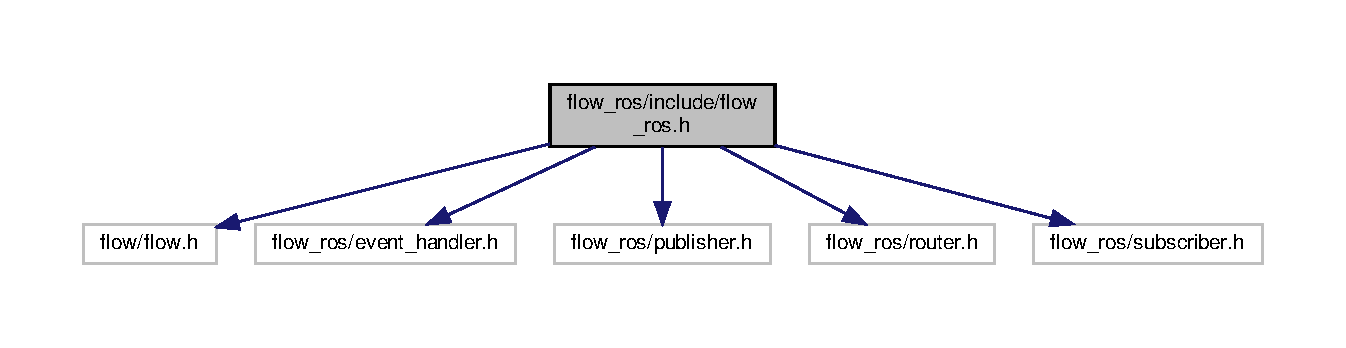
\includegraphics[width=350pt]{flow__ros_8h__incl}
\end{center}
\end{figure}


\subsection{Detailed Description}
\begin{DoxyCopyright}{Copyright}
2020 Fetch Robotics Inc. All rights reserved 
\end{DoxyCopyright}
\begin{DoxyAuthor}{Author}
Brian Cairl 
\end{DoxyAuthor}

\hypertarget{message__ptr_8h}{}\section{flow\+\_\+ros/include/message\+\_\+ptr.h File Reference}
\label{message__ptr_8h}\index{flow\+\_\+ros/include/message\+\_\+ptr.\+h@{flow\+\_\+ros/include/message\+\_\+ptr.\+h}}
{\ttfamily \#include $<$type\+\_\+traits$>$}\newline
{\ttfamily \#include $<$boost/shared\+\_\+ptr.\+hpp$>$}\newline
{\ttfamily \#include $<$ros/message\+\_\+traits.\+h$>$}\newline
{\ttfamily \#include $<$memory$>$}\newline
Include dependency graph for message\+\_\+ptr.\+h\+:\nopagebreak
\begin{figure}[H]
\begin{center}
\leavevmode
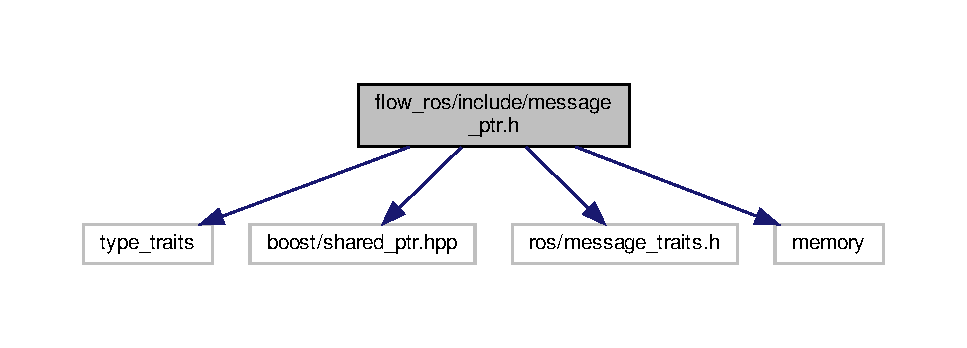
\includegraphics[width=350pt]{message__ptr_8h__incl}
\end{center}
\end{figure}
\subsection*{Classes}
\begin{DoxyCompactItemize}
\item 
struct \hyperlink{structflow__ros_1_1_message_shared_ptr_type}{flow\+\_\+ros\+::\+Message\+Shared\+Ptr\+Type$<$ Msg\+T, I\+S\+\_\+\+R\+O\+S\+\_\+\+M\+E\+S\+S\+A\+G\+E $>$}
\begin{DoxyCompactList}\small\item\em Traits object used to select correct shared\+\_\+ptr resource type. \end{DoxyCompactList}\item 
struct \hyperlink{structflow__ros_1_1_message_shared_const_ptr_type}{flow\+\_\+ros\+::\+Message\+Shared\+Const\+Ptr\+Type$<$ Msg\+T, I\+S\+\_\+\+R\+O\+S\+\_\+\+M\+E\+S\+S\+A\+G\+E $>$}
\begin{DoxyCompactList}\small\item\em Traits object used to select correct shared\+\_\+ptr const resource wrapper. \end{DoxyCompactList}\item 
struct \hyperlink{structflow__ros_1_1_message_shared_ptr_type_3_01_msg_t_00_01true_01_4}{flow\+\_\+ros\+::\+Message\+Shared\+Ptr\+Type$<$ Msg\+T, true $>$}
\begin{DoxyCompactList}\small\item\em Traits object used to select correct shared\+\_\+ptr resource type. \end{DoxyCompactList}\item 
struct \hyperlink{structflow__ros_1_1_message_shared_const_ptr_type_3_01_msg_t_00_01true_01_4}{flow\+\_\+ros\+::\+Message\+Shared\+Const\+Ptr\+Type$<$ Msg\+T, true $>$}
\begin{DoxyCompactList}\small\item\em Traits object used to select correct shared\+\_\+ptr const resource wrapper. \end{DoxyCompactList}\end{DoxyCompactItemize}
\subsection*{Namespaces}
\begin{DoxyCompactItemize}
\item 
 \hyperlink{namespaceflow__ros}{flow\+\_\+ros}
\end{DoxyCompactItemize}
\subsection*{Macros}
\begin{DoxyCompactItemize}
\item 
\#define \hyperlink{message__ptr_8h_a17fb2c81a1959d50ef0f0e0a31fcb667}{N\+O\+N\+\_\+\+R\+O\+S\+\_\+\+M\+E\+S\+S\+A\+G\+E\+\_\+\+S\+H\+A\+R\+E\+D\+\_\+\+P\+T\+R\+\_\+\+T\+M\+PL}~std\+::shared\+\_\+ptr$<$MsgT$>$
\end{DoxyCompactItemize}
\subsection*{Typedefs}
\begin{DoxyCompactItemize}
\item 
\mbox{\Hypertarget{namespaceflow__ros_aa27be896eb2c4c34fef0e9b7dd444d4c}\label{namespaceflow__ros_aa27be896eb2c4c34fef0e9b7dd444d4c}} 
{\footnotesize template$<$typename MsgT $>$ }\\using \hyperlink{namespaceflow__ros_aa27be896eb2c4c34fef0e9b7dd444d4c}{flow\+\_\+ros\+::non\+\_\+message\+\_\+shared\+\_\+ptr\+\_\+t} = \hyperlink{message__ptr_8h_a17fb2c81a1959d50ef0f0e0a31fcb667}{N\+O\+N\+\_\+\+R\+O\+S\+\_\+\+M\+E\+S\+S\+A\+G\+E\+\_\+\+S\+H\+A\+R\+E\+D\+\_\+\+P\+T\+R\+\_\+\+T\+M\+PL}
\begin{DoxyCompactList}\small\item\em Non-\/message resource pointer alias. \end{DoxyCompactList}\item 
\mbox{\Hypertarget{namespaceflow__ros_a21a684f38ee2083b3858613317c46d82}\label{namespaceflow__ros_a21a684f38ee2083b3858613317c46d82}} 
{\footnotesize template$<$typename MsgT $>$ }\\using \hyperlink{namespaceflow__ros_a21a684f38ee2083b3858613317c46d82}{flow\+\_\+ros\+::message\+\_\+shared\+\_\+ptr\+\_\+t} = typename Message\+Shared\+Ptr\+Type$<$ MsgT $>$\+::type
\begin{DoxyCompactList}\small\item\em Extracts appropriate shared\+\_\+ptr wrapper type for {\ttfamily MsgT} \end{DoxyCompactList}\item 
\mbox{\Hypertarget{namespaceflow__ros_ad222b6c2bd0341c551129c3a03241ad7}\label{namespaceflow__ros_ad222b6c2bd0341c551129c3a03241ad7}} 
{\footnotesize template$<$typename MsgT $>$ }\\using \hyperlink{namespaceflow__ros_ad222b6c2bd0341c551129c3a03241ad7}{flow\+\_\+ros\+::message\+\_\+shared\+\_\+const\+\_\+ptr\+\_\+t} = typename Message\+Shared\+Const\+Ptr\+Type$<$ MsgT $>$\+::type
\begin{DoxyCompactList}\small\item\em Extracts appropriate shared\+\_\+ptr wrapper type for {\ttfamily MsgT} \end{DoxyCompactList}\end{DoxyCompactItemize}
\subsection*{Variables}
\begin{DoxyCompactItemize}
\item 
\mbox{\Hypertarget{namespaceflow__ros_a9628f8bb8243036a41bcf1639e7ba57a}\label{namespaceflow__ros_a9628f8bb8243036a41bcf1639e7ba57a}} 
{\footnotesize template$<$typename MsgT $>$ }\\constexpr bool \hyperlink{namespaceflow__ros_a9628f8bb8243036a41bcf1639e7ba57a}{flow\+\_\+ros\+::is\+\_\+message\+\_\+v} = ros\+::message\+\_\+traits\+::\+Is\+Message$<$std\+::remove\+\_\+const\+\_\+t$<$MsgT$>$$>$\+::value
\begin{DoxyCompactList}\small\item\em Checks if object is a R\+OS message. \end{DoxyCompactList}\end{DoxyCompactItemize}


\subsection{Detailed Description}
\begin{DoxyCopyright}{Copyright}
2020 Fetch Robotics Inc. All rights reserved 
\end{DoxyCopyright}
\begin{DoxyAuthor}{Author}
Brian Cairl 
\end{DoxyAuthor}


\subsection{Macro Definition Documentation}
\mbox{\Hypertarget{message__ptr_8h_a17fb2c81a1959d50ef0f0e0a31fcb667}\label{message__ptr_8h_a17fb2c81a1959d50ef0f0e0a31fcb667}} 
\index{message\+\_\+ptr.\+h@{message\+\_\+ptr.\+h}!N\+O\+N\+\_\+\+R\+O\+S\+\_\+\+M\+E\+S\+S\+A\+G\+E\+\_\+\+S\+H\+A\+R\+E\+D\+\_\+\+P\+T\+R\+\_\+\+T\+M\+PL@{N\+O\+N\+\_\+\+R\+O\+S\+\_\+\+M\+E\+S\+S\+A\+G\+E\+\_\+\+S\+H\+A\+R\+E\+D\+\_\+\+P\+T\+R\+\_\+\+T\+M\+PL}}
\index{N\+O\+N\+\_\+\+R\+O\+S\+\_\+\+M\+E\+S\+S\+A\+G\+E\+\_\+\+S\+H\+A\+R\+E\+D\+\_\+\+P\+T\+R\+\_\+\+T\+M\+PL@{N\+O\+N\+\_\+\+R\+O\+S\+\_\+\+M\+E\+S\+S\+A\+G\+E\+\_\+\+S\+H\+A\+R\+E\+D\+\_\+\+P\+T\+R\+\_\+\+T\+M\+PL}!message\+\_\+ptr.\+h@{message\+\_\+ptr.\+h}}
\subsubsection{\texorpdfstring{N\+O\+N\+\_\+\+R\+O\+S\+\_\+\+M\+E\+S\+S\+A\+G\+E\+\_\+\+S\+H\+A\+R\+E\+D\+\_\+\+P\+T\+R\+\_\+\+T\+M\+PL}{NON\_ROS\_MESSAGE\_SHARED\_PTR\_TMPL}}
{\footnotesize\ttfamily \#define N\+O\+N\+\_\+\+R\+O\+S\+\_\+\+M\+E\+S\+S\+A\+G\+E\+\_\+\+S\+H\+A\+R\+E\+D\+\_\+\+P\+T\+R\+\_\+\+T\+M\+PL~std\+::shared\+\_\+ptr$<$MsgT$>$}

R\+OS messages are stored as {\ttfamily boost\+::shared\+\_\+ptr} resources, which was a design decision made before C++ had introduce {\ttfamily std\+::shared\+\_\+ptr} with C++11.

This definition provides a fall-\/back for non-\/message entities passed between \hyperlink{namespaceflow__ros}{flow\+\_\+ros} Publisher and Subscriber objects through local message passing using \hyperlink{classflow__ros_1_1_router}{flow\+\_\+ros\+::\+Router}, since there is no restriction to use boost in these cases.

If you would like to use {\ttfamily boost\+::shared\+\_\+ptr}, or something else, define {\ttfamily N\+O\+N\+\_\+\+R\+O\+S\+\_\+\+M\+E\+S\+S\+A\+G\+E\+\_\+\+S\+H\+A\+R\+E\+D\+\_\+\+P\+T\+R\+\_\+\+T\+M\+PL = {\itshape shared\+\_\+ptr}} before this point 
\hypertarget{message__seq__access_8h}{}\section{flow\+\_\+ros/include/message\+\_\+seq\+\_\+access.h File Reference}
\label{message__seq__access_8h}\index{flow\+\_\+ros/include/message\+\_\+seq\+\_\+access.\+h@{flow\+\_\+ros/include/message\+\_\+seq\+\_\+access.\+h}}
{\ttfamily \#include $<$cstdint$>$}\newline
{\ttfamily \#include $<$memory$>$}\newline
{\ttfamily \#include $<$type\+\_\+traits$>$}\newline
{\ttfamily \#include $<$vector$>$}\newline
{\ttfamily \#include $<$boost/shared\+\_\+ptr.\+hpp$>$}\newline
{\ttfamily \#include $<$ros/message\+\_\+traits.\+h$>$}\newline
{\ttfamily \#include $<$ros/time.\+h$>$}\newline
{\ttfamily \#include $<$flow/dispatch.\+h$>$}\newline
{\ttfamily \#include $<$flow\+\_\+ros/message\+\_\+ptr.\+h$>$}\newline
Include dependency graph for message\+\_\+seq\+\_\+access.\+h\+:\nopagebreak
\begin{figure}[H]
\begin{center}
\leavevmode
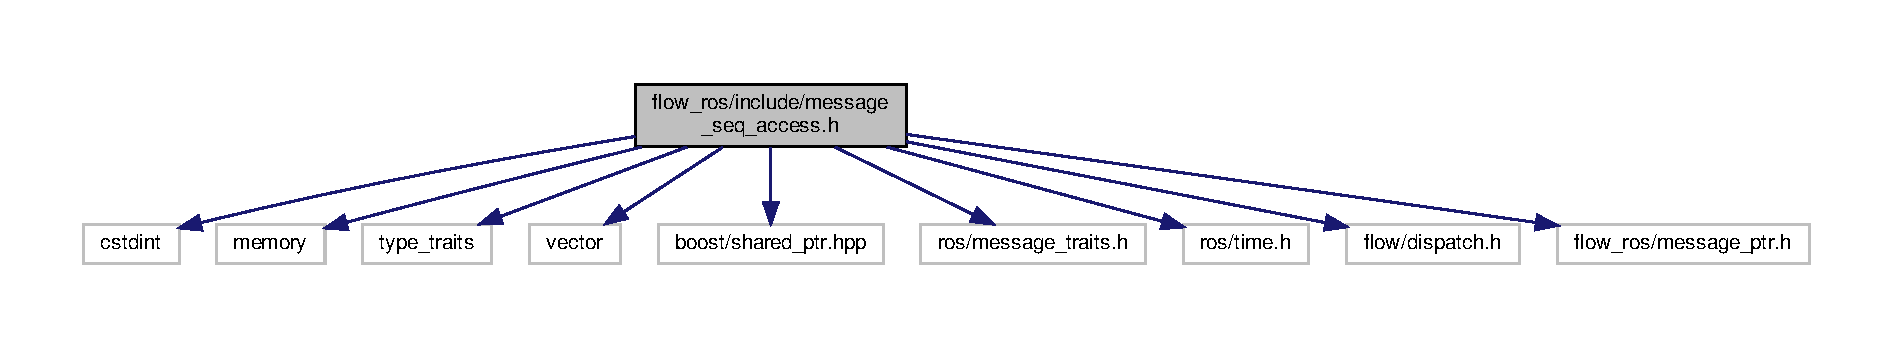
\includegraphics[width=350pt]{message__seq__access_8h__incl}
\end{center}
\end{figure}
\subsection*{Classes}
\begin{DoxyCompactItemize}
\item 
struct \hyperlink{structflow__ros_1_1_stamp_setter}{flow\+\_\+ros\+::\+Stamp\+Setter$<$ Msg\+T $>$}
\begin{DoxyCompactList}\small\item\em Helper object use to set message stamps. \end{DoxyCompactList}\item 
struct \hyperlink{structflow__ros_1_1_default_message_seq_dispatch_access}{flow\+\_\+ros\+::\+Default\+Message\+Seq\+Dispatch\+Access}
\begin{DoxyCompactList}\small\item\em Defines default message accessors to use a fall-\/back when defining {\ttfamily \hyperlink{structflow_1_1_dispatch_access}{flow\+::\+Dispatch\+Access}} \end{DoxyCompactList}\item 
struct \hyperlink{structflow_1_1_dispatch_traits_3_01boost_1_1shared__ptr_3_01const_01_msg_t_01_4_01_4}{flow\+::\+Dispatch\+Traits$<$ boost\+::shared\+\_\+ptr$<$ const Msg\+T $>$ $>$}
\begin{DoxyCompactList}\small\item\em Default R\+OS message Dispatch traits. \end{DoxyCompactList}\item 
struct \hyperlink{structflow_1_1_dispatch_traits_3_01std_1_1shared__ptr_3_01const_01_msg_t_01_4_01_4}{flow\+::\+Dispatch\+Traits$<$ std\+::shared\+\_\+ptr$<$ const Msg\+T $>$ $>$}
\begin{DoxyCompactList}\small\item\em Default R\+OS message-\/like Dispatch traits. \end{DoxyCompactList}\item 
struct \hyperlink{structflow_1_1_dispatch_access}{flow\+::\+Dispatch\+Access$<$ Msg\+T $>$}
\begin{DoxyCompactList}\small\item\em Template which basic methods for Message\+Dispatch. \end{DoxyCompactList}\end{DoxyCompactItemize}
\subsection*{Namespaces}
\begin{DoxyCompactItemize}
\item 
 \hyperlink{namespaceflow__ros}{flow\+\_\+ros}
\end{DoxyCompactItemize}


\subsection{Detailed Description}
\begin{DoxyCopyright}{Copyright}
2020 Fetch Robotics Inc. All rights reserved 
\end{DoxyCopyright}
\begin{DoxyAuthor}{Author}
Brian Cairl 
\end{DoxyAuthor}

\hypertarget{message__stamp__access_8h}{}\section{flow\+\_\+ros/include/message\+\_\+stamp\+\_\+access.h File Reference}
\label{message__stamp__access_8h}\index{flow\+\_\+ros/include/message\+\_\+stamp\+\_\+access.\+h@{flow\+\_\+ros/include/message\+\_\+stamp\+\_\+access.\+h}}
{\ttfamily \#include $<$memory$>$}\newline
{\ttfamily \#include $<$type\+\_\+traits$>$}\newline
{\ttfamily \#include $<$vector$>$}\newline
{\ttfamily \#include $<$boost/shared\+\_\+ptr.\+hpp$>$}\newline
{\ttfamily \#include $<$ros/time.\+h$>$}\newline
{\ttfamily \#include $<$flow/dispatch.\+h$>$}\newline
{\ttfamily \#include $<$flow\+\_\+ros/message\+\_\+ptr.\+h$>$}\newline
Include dependency graph for message\+\_\+stamp\+\_\+access.\+h\+:\nopagebreak
\begin{figure}[H]
\begin{center}
\leavevmode
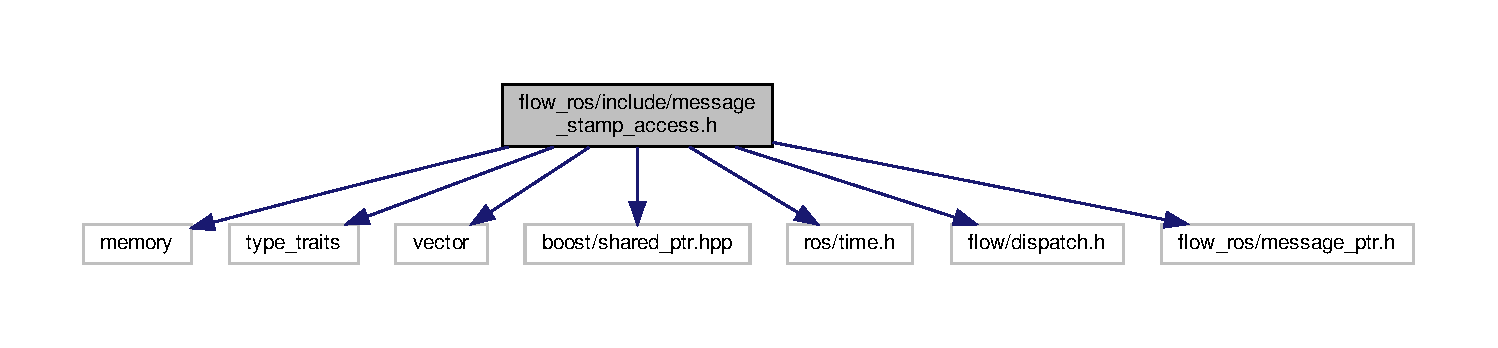
\includegraphics[width=350pt]{message__stamp__access_8h__incl}
\end{center}
\end{figure}
\subsection*{Classes}
\begin{DoxyCompactItemize}
\item 
struct \hyperlink{structflow__ros_1_1_stamp_setter}{flow\+\_\+ros\+::\+Stamp\+Setter$<$ Msg\+T $>$}
\begin{DoxyCompactList}\small\item\em Helper object use to set message stamps. \end{DoxyCompactList}\item 
struct \hyperlink{structflow__ros_1_1_default_message_stamp_dispatch_access}{flow\+\_\+ros\+::\+Default\+Message\+Stamp\+Dispatch\+Access}
\begin{DoxyCompactList}\small\item\em Defines default message accessors to use a fall-\/back when defining {\ttfamily \hyperlink{structflow_1_1_dispatch_access}{flow\+::\+Dispatch\+Access}} \end{DoxyCompactList}\item 
struct \hyperlink{structflow_1_1_stamp_traits_3_01ros_1_1_time_01_4}{flow\+::\+Stamp\+Traits$<$ ros\+::\+Time $>$}
\begin{DoxyCompactList}\small\item\em R\+OS timing type traits for associated message Dispatch. \end{DoxyCompactList}\item 
struct \hyperlink{structflow_1_1_dispatch_traits_3_01boost_1_1shared__ptr_3_01const_01_msg_t_01_4_01_4}{flow\+::\+Dispatch\+Traits$<$ boost\+::shared\+\_\+ptr$<$ const Msg\+T $>$ $>$}
\begin{DoxyCompactList}\small\item\em Default R\+OS message Dispatch traits. \end{DoxyCompactList}\item 
struct \hyperlink{structflow_1_1_dispatch_traits_3_01std_1_1shared__ptr_3_01const_01_msg_t_01_4_01_4}{flow\+::\+Dispatch\+Traits$<$ std\+::shared\+\_\+ptr$<$ const Msg\+T $>$ $>$}
\begin{DoxyCompactList}\small\item\em Default R\+OS message-\/like Dispatch traits. \end{DoxyCompactList}\item 
struct \hyperlink{structflow_1_1_dispatch_access}{flow\+::\+Dispatch\+Access$<$ Msg\+T $>$}
\begin{DoxyCompactList}\small\item\em Template which basic methods for Message\+Dispatch. \end{DoxyCompactList}\end{DoxyCompactItemize}
\subsection*{Namespaces}
\begin{DoxyCompactItemize}
\item 
 \hyperlink{namespaceflow__ros}{flow\+\_\+ros}
\end{DoxyCompactItemize}
\subsection*{Functions}
\begin{DoxyCompactItemize}
\item 
{\footnotesize template$<$typename MsgT $>$ }\\void \hyperlink{namespaceflow__ros_a4ee9a96308b9612ffbf1c133dacd91e2}{flow\+\_\+ros\+::set\+\_\+stamp} (MsgT \&\&msg, const ros\+::\+Time \&stamp)
\begin{DoxyCompactList}\small\item\em Helper function use to set message stamp with \hyperlink{structflow__ros_1_1_stamp_setter}{Stamp\+Setter}. \end{DoxyCompactList}\end{DoxyCompactItemize}


\subsection{Detailed Description}
\begin{DoxyCopyright}{Copyright}
2020 Fetch Robotics Inc. All rights reserved 
\end{DoxyCopyright}
\begin{DoxyAuthor}{Author}
Brian Cairl 
\end{DoxyAuthor}

\hypertarget{publisher_8h}{}\section{flow\+\_\+ros/include/publisher.h File Reference}
\label{publisher_8h}\index{flow\+\_\+ros/include/publisher.\+h@{flow\+\_\+ros/include/publisher.\+h}}
{\ttfamily \#include $<$cstdint$>$}\newline
{\ttfamily \#include $<$memory$>$}\newline
{\ttfamily \#include $<$stdexcept$>$}\newline
{\ttfamily \#include $<$string$>$}\newline
{\ttfamily \#include $<$vector$>$}\newline
{\ttfamily \#include $<$ros/node\+\_\+handle.\+h$>$}\newline
{\ttfamily \#include $<$ros/publisher.\+h$>$}\newline
{\ttfamily \#include $<$flow/impl/static\+\_\+assert.\+hpp$>$}\newline
{\ttfamily \#include $<$flow\+\_\+ros/message\+\_\+ptr.\+h$>$}\newline
{\ttfamily \#include $<$flow\+\_\+ros/router.\+h$>$}\newline
{\ttfamily \#include $<$flow\+\_\+ros/routing/local\+\_\+publication.\+h$>$}\newline
{\ttfamily \#include $<$flow\+\_\+ros/routing/publication\+\_\+wrapper.\+h$>$}\newline
{\ttfamily \#include $<$flow\+\_\+ros/routing/ros\+\_\+publication.\+h$>$}\newline
Include dependency graph for publisher.\+h\+:\nopagebreak
\begin{figure}[H]
\begin{center}
\leavevmode
\includegraphics[width=350pt]{publisher_8h__incl}
\end{center}
\end{figure}
\subsection*{Classes}
\begin{DoxyCompactItemize}
\item 
class \hyperlink{classflow__ros_1_1_publisher_base}{flow\+\_\+ros\+::\+Publisher\+Base}
\begin{DoxyCompactList}\small\item\em Publish base to expose meta-\/information methods. \end{DoxyCompactList}\item 
class \hyperlink{classflow__ros_1_1_publisher_output_base}{flow\+\_\+ros\+::\+Publisher\+Output\+Base$<$ Msg\+T $>$}
\begin{DoxyCompactList}\small\item\em Message publisher base type. \end{DoxyCompactList}\item 
class \hyperlink{classflow__ros_1_1_publisher}{flow\+\_\+ros\+::\+Publisher$<$ Msg\+T $>$}
\begin{DoxyCompactList}\small\item\em Output channel which publishes messages. \end{DoxyCompactList}\item 
class \hyperlink{classflow__ros_1_1_multi_publisher}{flow\+\_\+ros\+::\+Multi\+Publisher$<$ Msg\+T, Output\+Container\+T $>$}
\begin{DoxyCompactList}\small\item\em Output channel specialization which publishes multiple messages. \end{DoxyCompactList}\item 
struct \hyperlink{structflow__ros_1_1_publisher_traits}{flow\+\_\+ros\+::\+Publisher\+Traits$<$ Msg\+T $>$}
\begin{DoxyCompactList}\small\item\em \hyperlink{classflow__ros_1_1_publisher}{Publisher} type traits. \end{DoxyCompactList}\item 
struct \hyperlink{structflow__ros_1_1_publisher_traits_3_01_publisher_3_01_msg_t_01_4_01_4}{flow\+\_\+ros\+::\+Publisher\+Traits$<$ Publisher$<$ Msg\+T $>$ $>$}
\begin{DoxyCompactList}\small\item\em \hyperlink{classflow__ros_1_1_publisher}{Publisher} type traits. \end{DoxyCompactList}\item 
struct \hyperlink{structflow__ros_1_1_publisher_traits_3_01_multi_publisher_3_01_msg_t_00_01_output_container_t_01_4_01_4}{flow\+\_\+ros\+::\+Publisher\+Traits$<$ Multi\+Publisher$<$ Msg\+T, Output\+Container\+T $>$ $>$}
\begin{DoxyCompactList}\small\item\em \hyperlink{classflow__ros_1_1_publisher}{Publisher} type traits. \end{DoxyCompactList}\end{DoxyCompactItemize}
\subsection*{Namespaces}
\begin{DoxyCompactItemize}
\item 
 \hyperlink{namespaceflow__ros}{flow\+\_\+ros}
\end{DoxyCompactItemize}


\subsection{Detailed Description}
\begin{DoxyCopyright}{Copyright}
2020 Fetch Robotics Inc. All rights reserved 
\end{DoxyCopyright}
\begin{DoxyAuthor}{Author}
Brian Cairl 
\end{DoxyAuthor}

\hypertarget{router_8h}{}\section{flow\+\_\+ros/include/router.h File Reference}
\label{router_8h}\index{flow\+\_\+ros/include/router.\+h@{flow\+\_\+ros/include/router.\+h}}
{\ttfamily \#include $<$memory$>$}\newline
{\ttfamily \#include $<$mutex$>$}\newline
{\ttfamily \#include $<$ostream$>$}\newline
{\ttfamily \#include $<$sstream$>$}\newline
{\ttfamily \#include $<$stdexcept$>$}\newline
{\ttfamily \#include $<$string$>$}\newline
{\ttfamily \#include $<$thread$>$}\newline
{\ttfamily \#include $<$type\+\_\+traits$>$}\newline
{\ttfamily \#include $<$unordered\+\_\+map$>$}\newline
{\ttfamily \#include $<$utility$>$}\newline
{\ttfamily \#include $<$rosbag/message\+\_\+instance.\+h$>$}\newline
{\ttfamily \#include $<$flow\+\_\+ros/message\+\_\+ptr.\+h$>$}\newline
{\ttfamily \#include $<$flow\+\_\+ros/routing/local\+\_\+publication.\+h$>$}\newline
{\ttfamily \#include $<$flow\+\_\+ros/routing/local\+\_\+subscription.\+h$>$}\newline
{\ttfamily \#include $<$flow\+\_\+ros/routing/publication\+\_\+wrapper.\+h$>$}\newline
{\ttfamily \#include $<$flow\+\_\+ros/routing/subscription\+\_\+wrapper.\+h$>$}\newline
Include dependency graph for router.\+h\+:\nopagebreak
\begin{figure}[H]
\begin{center}
\leavevmode
\includegraphics[width=350pt]{router_8h__incl}
\end{center}
\end{figure}
\subsection*{Classes}
\begin{DoxyCompactItemize}
\item 
class \hyperlink{classflow__ros_1_1_unknown_subscription_error}{flow\+\_\+ros\+::\+Unknown\+Subscription\+Error}
\begin{DoxyCompactList}\small\item\em Exception thrown when message for an unknown subscription is injected. \end{DoxyCompactList}\item 
class \hyperlink{classflow__ros_1_1_router}{flow\+\_\+ros\+::\+Router}
\begin{DoxyCompactList}\small\item\em An in-\/process message routing object. \end{DoxyCompactList}\end{DoxyCompactItemize}
\subsection*{Namespaces}
\begin{DoxyCompactItemize}
\item 
 \hyperlink{namespaceflow__ros}{flow\+\_\+ros}
\end{DoxyCompactItemize}


\subsection{Detailed Description}
\begin{DoxyCopyright}{Copyright}
2020 Fetch Robotics Inc. All rights reserved 
\end{DoxyCopyright}
\begin{DoxyAuthor}{Author}
Brian Cairl 
\end{DoxyAuthor}

\hypertarget{local__subscription_8h}{}\section{flow\+\_\+ros/include/routing/local\+\_\+subscription.h File Reference}
\label{local__subscription_8h}\index{flow\+\_\+ros/include/routing/local\+\_\+subscription.\+h@{flow\+\_\+ros/include/routing/local\+\_\+subscription.\+h}}
{\ttfamily \#include $<$cstdint$>$}\newline
{\ttfamily \#include $<$functional$>$}\newline
{\ttfamily \#include $<$memory$>$}\newline
{\ttfamily \#include $<$sstream$>$}\newline
{\ttfamily \#include $<$stdexcept$>$}\newline
{\ttfamily \#include $<$string$>$}\newline
{\ttfamily \#include $<$type\+\_\+traits$>$}\newline
{\ttfamily \#include $<$utility$>$}\newline
{\ttfamily \#include $<$rosbag/message\+\_\+instance.\+h$>$}\newline
{\ttfamily \#include $<$flow\+\_\+ros/routing/subscription\+\_\+wrapper.\+h$>$}\newline
Include dependency graph for local\+\_\+subscription.\+h\+:\nopagebreak
\begin{figure}[H]
\begin{center}
\leavevmode
\includegraphics[width=350pt]{local__subscription_8h__incl}
\end{center}
\end{figure}
\subsection*{Classes}
\begin{DoxyCompactItemize}
\item 
class \hyperlink{classflow__ros_1_1routing_1_1_message_instance_error}{flow\+\_\+ros\+::routing\+::\+Message\+Instance\+Error}
\begin{DoxyCompactList}\small\item\em Exception thrown when a message cannot be instanced from {\ttfamily rosbag\+::\+Message\+Instance} \end{DoxyCompactList}\item 
class \hyperlink{classflow__ros_1_1routing_1_1_message_type_error}{flow\+\_\+ros\+::routing\+::\+Message\+Type\+Error}
\begin{DoxyCompactList}\small\item\em Exception thrown when a message type does not match for a given topic. \end{DoxyCompactList}\item 
class \hyperlink{classflow__ros_1_1routing_1_1_local_subscription_base}{flow\+\_\+ros\+::routing\+::\+Local\+Subscription\+Base}
\begin{DoxyCompactList}\small\item\em \hyperlink{classflow__ros_1_1routing_1_1_local_subscription}{Local\+Subscription} base which provides basic info and erases Msg\+T-\/dependent methods. \end{DoxyCompactList}\item 
class \hyperlink{classflow__ros_1_1routing_1_1_local_subscription}{flow\+\_\+ros\+::routing\+::\+Local\+Subscription$<$ Msg\+T $>$}
\item 
class \hyperlink{classflow__ros_1_1routing_1_1_local_subscription_group}{flow\+\_\+ros\+::routing\+::\+Local\+Subscription\+Group}
\begin{DoxyCompactList}\small\item\em Holds a group of \hyperlink{classflow__ros_1_1routing_1_1_local_subscription}{Local\+Subscription} objects associated with a particular topic. \end{DoxyCompactList}\end{DoxyCompactItemize}
\subsection*{Namespaces}
\begin{DoxyCompactItemize}
\item 
 \hyperlink{namespaceflow__ros}{flow\+\_\+ros}
\end{DoxyCompactItemize}


\subsection{Detailed Description}
\begin{DoxyCopyright}{Copyright}
2020 Fetch Robotics Inc. All rights reserved 
\end{DoxyCopyright}
\begin{DoxyAuthor}{Author}
Brian Cairl 
\end{DoxyAuthor}

\hypertarget{subscription__wrapper_8h}{}\section{flow\+\_\+ros/include/routing/subscription\+\_\+wrapper.h File Reference}
\label{subscription__wrapper_8h}\index{flow\+\_\+ros/include/routing/subscription\+\_\+wrapper.\+h@{flow\+\_\+ros/include/routing/subscription\+\_\+wrapper.\+h}}
{\ttfamily \#include $<$cstdint$>$}\newline
{\ttfamily \#include $<$string$>$}\newline
{\ttfamily \#include $<$flow/impl/implement\+\_\+crtp\+\_\+base.\+hpp$>$}\newline
{\ttfamily \#include $<$flow\+\_\+ros/routing/transport\+\_\+info.\+h$>$}\newline
Include dependency graph for subscription\+\_\+wrapper.\+h\+:\nopagebreak
\begin{figure}[H]
\begin{center}
\leavevmode
\includegraphics[width=350pt]{subscription__wrapper_8h__incl}
\end{center}
\end{figure}
\subsection*{Classes}
\begin{DoxyCompactItemize}
\item 
class \hyperlink{classflow__ros_1_1routing_1_1_subscription_wrapper}{flow\+\_\+ros\+::routing\+::\+Subscription\+Wrapper}
\begin{DoxyCompactList}\small\item\em Base for message subscribing implementation. \end{DoxyCompactList}\end{DoxyCompactItemize}
\subsection*{Namespaces}
\begin{DoxyCompactItemize}
\item 
 \hyperlink{namespaceflow__ros}{flow\+\_\+ros}
\end{DoxyCompactItemize}


\subsection{Detailed Description}
\begin{DoxyCopyright}{Copyright}
2020 Fetch Robotics Inc. All rights reserved 
\end{DoxyCopyright}
\begin{DoxyAuthor}{Author}
Brian Cairl 
\end{DoxyAuthor}

\hypertarget{transport__info_8h}{}\section{flow\+\_\+ros/include/routing/transport\+\_\+info.h File Reference}
\label{transport__info_8h}\index{flow\+\_\+ros/include/routing/transport\+\_\+info.\+h@{flow\+\_\+ros/include/routing/transport\+\_\+info.\+h}}
\subsection*{Namespaces}
\begin{DoxyCompactItemize}
\item 
 \hyperlink{namespaceflow__ros}{flow\+\_\+ros}
\end{DoxyCompactItemize}
\subsection*{Enumerations}
\begin{DoxyCompactItemize}
\item 
\mbox{\Hypertarget{transport__info_8h_ae57afcf849a5bdb82b958347c6ccc57b}\label{transport__info_8h_ae57afcf849a5bdb82b958347c6ccc57b}} 
enum \hyperlink{transport__info_8h_ae57afcf849a5bdb82b958347c6ccc57b}{flow\+\_\+ros\+::routing\+::\+Transport\+Method} \+: int \{ {\bfseries flow\+\_\+ros\+::routing\+::\+Transport\+Method\+::\+U\+N\+K\+N\+O\+WN}, 
{\bfseries flow\+\_\+ros\+::routing\+::\+Transport\+Method\+::\+M\+U\+L\+TI}, 
{\bfseries flow\+\_\+ros\+::routing\+::\+Transport\+Method\+::\+L\+O\+C\+AL}, 
{\bfseries flow\+\_\+ros\+::routing\+::\+Transport\+Method\+::\+R\+OS}
 \}\begin{DoxyCompactList}\small\item\em Transport method codes. \end{DoxyCompactList}
\item 
\mbox{\Hypertarget{transport__info_8h_acb4b6ac875de32a0d0ee8cec235f7752}\label{transport__info_8h_acb4b6ac875de32a0d0ee8cec235f7752}} 
enum \hyperlink{transport__info_8h_acb4b6ac875de32a0d0ee8cec235f7752}{flow\+\_\+ros\+::routing\+::\+Direction} \+: int \{ {\bfseries flow\+\_\+ros\+::routing\+::\+Direction\+::\+U\+N\+K\+N\+O\+WN}, 
{\bfseries flow\+\_\+ros\+::routing\+::\+Direction\+::\+I\+N\+B\+O\+U\+ND}, 
{\bfseries flow\+\_\+ros\+::routing\+::\+Direction\+::\+O\+U\+T\+B\+O\+U\+ND}
 \}\begin{DoxyCompactList}\small\item\em Transport direction codes. \end{DoxyCompactList}
\end{DoxyCompactItemize}


\subsection{Detailed Description}
\begin{DoxyCopyright}{Copyright}
2020 Fetch Robotics Inc. All rights reserved 
\end{DoxyCopyright}
\begin{DoxyAuthor}{Author}
Brian Cairl 
\end{DoxyAuthor}

\hypertarget{transport__info__ostream_8h}{}\section{flow\+\_\+ros/include/routing/transport\+\_\+info\+\_\+ostream.h File Reference}
\label{transport__info__ostream_8h}\index{flow\+\_\+ros/include/routing/transport\+\_\+info\+\_\+ostream.\+h@{flow\+\_\+ros/include/routing/transport\+\_\+info\+\_\+ostream.\+h}}
{\ttfamily \#include $<$ostream$>$}\newline
Include dependency graph for transport\+\_\+info\+\_\+ostream.\+h\+:\nopagebreak
\begin{figure}[H]
\begin{center}
\leavevmode
\includegraphics[width=208pt]{transport__info__ostream_8h__incl}
\end{center}
\end{figure}
\subsection*{Namespaces}
\begin{DoxyCompactItemize}
\item 
 \hyperlink{namespaceflow__ros}{flow\+\_\+ros}
\end{DoxyCompactItemize}
\subsection*{Functions}
\begin{DoxyCompactItemize}
\item 
std\+::ostream \& \hyperlink{transport__info__ostream_8h_a8c2b486f346443e35a4b9ca12f557f9f}{flow\+\_\+ros\+::routing\+::operator$<$$<$} (std\+::ostream \&os, const Transport\+Method \&transport)
\begin{DoxyCompactList}\small\item\em Output stream overload for {\ttfamily flow\+\_\+ros\+::routing\+::\+Transport\+Method} \end{DoxyCompactList}\item 
std\+::ostream \& \hyperlink{transport__info__ostream_8h_a19d2a660ed95cbe90ede010a5e945c94}{flow\+\_\+ros\+::routing\+::operator$<$$<$} (std\+::ostream \&os, const Direction \&direction)
\begin{DoxyCompactList}\small\item\em Output stream overload for {\ttfamily flow\+\_\+ros\+::routing\+::\+Direction} \end{DoxyCompactList}\end{DoxyCompactItemize}


\subsection{Detailed Description}
\begin{DoxyCopyright}{Copyright}
2020 Fetch Robotics Inc. All rights reserved 
\end{DoxyCopyright}
\begin{DoxyAuthor}{Author}
Brian Cairl 
\end{DoxyAuthor}


\subsection{Function Documentation}
\mbox{\Hypertarget{transport__info__ostream_8h_file_a8c2b486f346443e35a4b9ca12f557f9f}\label{transport__info__ostream_8h_file_a8c2b486f346443e35a4b9ca12f557f9f}} 
\index{transport\+\_\+info\+\_\+ostream.\+h@{transport\+\_\+info\+\_\+ostream.\+h}!operator$<$$<$@{operator$<$$<$}}
\index{operator$<$$<$@{operator$<$$<$}!transport\+\_\+info\+\_\+ostream.\+h@{transport\+\_\+info\+\_\+ostream.\+h}}
\subsubsection{\texorpdfstring{operator$<$$<$()}{operator<<()}\hspace{0.1cm}{\footnotesize\ttfamily [1/2]}}
{\footnotesize\ttfamily std\+::ostream\& flow\+\_\+ros\+::routing\+::operator$<$$<$ (\begin{DoxyParamCaption}\item[{std\+::ostream \&}]{os,  }\item[{const \hyperlink{transport__info_8h_ae57afcf849a5bdb82b958347c6ccc57b}{Transport\+Method} \&}]{transport }\end{DoxyParamCaption})\hspace{0.3cm}{\ttfamily [inline]}}



Output stream overload for {\ttfamily flow\+\_\+ros\+::routing\+::\+Transport\+Method} 


\begin{DoxyParams}[1]{Parameters}
\mbox{\tt in,out}  & {\em os} & output stream \\
\hline
 & {\em transport} & transport info enum\\
\hline
\end{DoxyParams}
\begin{DoxyReturn}{Returns}
os 
\end{DoxyReturn}
\mbox{\Hypertarget{transport__info__ostream_8h_file_a19d2a660ed95cbe90ede010a5e945c94}\label{transport__info__ostream_8h_file_a19d2a660ed95cbe90ede010a5e945c94}} 
\index{transport\+\_\+info\+\_\+ostream.\+h@{transport\+\_\+info\+\_\+ostream.\+h}!operator$<$$<$@{operator$<$$<$}}
\index{operator$<$$<$@{operator$<$$<$}!transport\+\_\+info\+\_\+ostream.\+h@{transport\+\_\+info\+\_\+ostream.\+h}}
\subsubsection{\texorpdfstring{operator$<$$<$()}{operator<<()}\hspace{0.1cm}{\footnotesize\ttfamily [2/2]}}
{\footnotesize\ttfamily std\+::ostream\& flow\+\_\+ros\+::routing\+::operator$<$$<$ (\begin{DoxyParamCaption}\item[{std\+::ostream \&}]{os,  }\item[{const \hyperlink{transport__info_8h_acb4b6ac875de32a0d0ee8cec235f7752}{Direction} \&}]{direction }\end{DoxyParamCaption})\hspace{0.3cm}{\ttfamily [inline]}}



Output stream overload for {\ttfamily flow\+\_\+ros\+::routing\+::\+Direction} 


\begin{DoxyParams}[1]{Parameters}
\mbox{\tt in,out}  & {\em os} & output stream \\
\hline
 & {\em direction} & direction info enum\\
\hline
\end{DoxyParams}
\begin{DoxyReturn}{Returns}
os 
\end{DoxyReturn}

\hypertarget{subscriber_8h}{}\section{flow\+\_\+ros/include/subscriber.h File Reference}
\label{subscriber_8h}\index{flow\+\_\+ros/include/subscriber.\+h@{flow\+\_\+ros/include/subscriber.\+h}}
{\ttfamily \#include $<$algorithm$>$}\newline
{\ttfamily \#include $<$chrono$>$}\newline
{\ttfamily \#include $<$memory$>$}\newline
{\ttfamily \#include $<$string$>$}\newline
{\ttfamily \#include $<$thread$>$}\newline
{\ttfamily \#include $<$utility$>$}\newline
{\ttfamily \#include $<$ros/message\+\_\+traits.\+h$>$}\newline
{\ttfamily \#include $<$ros/node\+\_\+handle.\+h$>$}\newline
{\ttfamily \#include $<$ros/subscriber.\+h$>$}\newline
{\ttfamily \#include $<$flow/drivers.\+h$>$}\newline
{\ttfamily \#include $<$flow/followers.\+h$>$}\newline
{\ttfamily \#include $<$flow\+\_\+ros/message\+\_\+ptr.\+h$>$}\newline
{\ttfamily \#include $<$flow\+\_\+ros/router.\+h$>$}\newline
{\ttfamily \#include $<$flow\+\_\+ros/routing/local\+\_\+subscription.\+h$>$}\newline
{\ttfamily \#include $<$flow\+\_\+ros/routing/ros\+\_\+subscription.\+h$>$}\newline
{\ttfamily \#include $<$flow\+\_\+ros/routing/subscription\+\_\+wrapper.\+h$>$}\newline
Include dependency graph for subscriber.\+h\+:\nopagebreak
\begin{figure}[H]
\begin{center}
\leavevmode
\includegraphics[width=350pt]{subscriber_8h__incl}
\end{center}
\end{figure}
\subsection*{Classes}
\begin{DoxyCompactItemize}
\item 
class \hyperlink{classflow__ros_1_1_subscriber_base}{flow\+\_\+ros\+::\+Subscriber\+Base}
\begin{DoxyCompactList}\small\item\em Message input channel with meta information interfaces. \end{DoxyCompactList}\item 
class \hyperlink{classflow__ros_1_1_subscriber_policy_base}{flow\+\_\+ros\+::\+Subscriber\+Policy\+Base$<$ Policy\+T $>$}
\begin{DoxyCompactList}\small\item\em Message input channel with an associated capture policy. \end{DoxyCompactList}\item 
class \hyperlink{classflow__ros_1_1_subscriber}{flow\+\_\+ros\+::\+Subscriber$<$ Msg\+T, Policy\+Tmpl, Lock\+Policy\+T, Msg\+Const\+Ptr\+Container\+T $>$}
\begin{DoxyCompactList}\small\item\em Input channel which subscribes to messages. \end{DoxyCompactList}\item 
struct \hyperlink{structflow__ros_1_1_subscriber_traits}{flow\+\_\+ros\+::\+Subscriber\+Traits$<$ Msg\+T $>$}
\begin{DoxyCompactList}\small\item\em \hyperlink{classflow__ros_1_1_subscriber}{Subscriber} type traits. \end{DoxyCompactList}\item 
struct \hyperlink{structflow__ros_1_1_subscriber_traits_3_01_subscriber_3_01_msg_t_00_01_policy_tmpl_00_01_lock_policy_t_01_4_01_4}{flow\+\_\+ros\+::\+Subscriber\+Traits$<$ Subscriber$<$ Msg\+T, Policy\+Tmpl, Lock\+Policy\+T $>$ $>$}
\begin{DoxyCompactList}\small\item\em \hyperlink{classflow__ros_1_1_subscriber}{Subscriber} type traits. \end{DoxyCompactList}\item 
struct \hyperlink{structflow_1_1is__driver_3_1_1flow__ros_1_1_subscriber_3_01_msg_t_00_01_policy_tmpl_00_01_lock_policy_t_01_4_01_4}{flow\+::is\+\_\+driver$<$\+::flow\+\_\+ros\+::\+Subscriber$<$ Msg\+T, Policy\+Tmpl, Lock\+Policy\+T $>$ $>$}
\begin{DoxyCompactList}\small\item\em Checks if subscriber capture policy is derived from a Driver base. \end{DoxyCompactList}\item 
struct \hyperlink{structflow_1_1is__follower_3_1_1flow__ros_1_1_subscriber_3_01_msg_t_00_01_policy_tmpl_00_01_lock_policy_t_01_4_01_4}{flow\+::is\+\_\+follower$<$\+::flow\+\_\+ros\+::\+Subscriber$<$ Msg\+T, Policy\+Tmpl, Lock\+Policy\+T $>$ $>$}
\begin{DoxyCompactList}\small\item\em Checks if subscriber capture policy is derived from a Follower base. \end{DoxyCompactList}\item 
struct \hyperlink{structflow_1_1_captor_traits_3_1_1flow__ros_1_1_subscriber_policy_base_3_01_policy_t_01_4_01_4}{flow\+::\+Captor\+Traits$<$\+::flow\+\_\+ros\+::\+Subscriber\+Policy\+Base$<$ Policy\+T $>$ $>$}
\begin{DoxyCompactList}\small\item\em Captor traits associated with underlying Captor of Subscriber\+Policy\+Base. \end{DoxyCompactList}\item 
struct \hyperlink{structflow_1_1_captor_traits_3_1_1flow__ros_1_1_subscriber_3_01_msg_t_00_01_policy_tmpl_00_01_lock_policy_t_01_4_01_4}{flow\+::\+Captor\+Traits$<$\+::flow\+\_\+ros\+::\+Subscriber$<$ Msg\+T, Policy\+Tmpl, Lock\+Policy\+T $>$ $>$}
\begin{DoxyCompactList}\small\item\em Captor traits associated with underlying Captor of Subscriber. \end{DoxyCompactList}\end{DoxyCompactItemize}
\subsection*{Namespaces}
\begin{DoxyCompactItemize}
\item 
 \hyperlink{namespaceflow__ros}{flow\+\_\+ros}
\end{DoxyCompactItemize}


\subsection{Detailed Description}
\begin{DoxyCopyright}{Copyright}
2020 Fetch Robotics Inc. All rights reserved 
\end{DoxyCopyright}
\begin{DoxyAuthor}{Author}
Brian Cairl 
\end{DoxyAuthor}

\hypertarget{event__handler_8cpp}{}\section{flow\+\_\+ros/test/unit/event\+\_\+handler.cpp File Reference}
\label{event__handler_8cpp}\index{flow\+\_\+ros/test/unit/event\+\_\+handler.\+cpp@{flow\+\_\+ros/test/unit/event\+\_\+handler.\+cpp}}
{\ttfamily \#include $<$string$>$}\newline
{\ttfamily \#include $<$thread$>$}\newline
{\ttfamily \#include $<$gtest/gtest.\+h$>$}\newline
{\ttfamily \#include $<$std\+\_\+msgs/\+Header.\+h$>$}\newline
{\ttfamily \#include $<$flow/flow.\+h$>$}\newline
{\ttfamily \#include $<$flow\+\_\+ros/event\+\_\+handler.\+h$>$}\newline
{\ttfamily \#include $<$flow\+\_\+ros/event\+\_\+handler\+\_\+ostream.\+h$>$}\newline
{\ttfamily \#include $<$flow\+\_\+ros/message\+\_\+stamp\+\_\+access.\+h$>$}\newline
{\ttfamily \#include $<$flow\+\_\+ros/publisher.\+h$>$}\newline
{\ttfamily \#include $<$flow\+\_\+ros/subscriber.\+h$>$}\newline
Include dependency graph for event\+\_\+handler.\+cpp\+:\nopagebreak
\begin{figure}[H]
\begin{center}
\leavevmode
\includegraphics[width=350pt]{event__handler_8cpp__incl}
\end{center}
\end{figure}
\subsection*{Classes}
\begin{DoxyCompactItemize}
\item 
struct \hyperlink{struct_test_message1}{Test\+Message1}
\begin{DoxyCompactList}\small\item\em A R\+OS messages-\/like object. \end{DoxyCompactList}\item 
struct \hyperlink{struct_test_message2}{Test\+Message2}
\end{DoxyCompactItemize}
\subsection*{Functions}
\begin{DoxyCompactItemize}
\item 
\mbox{\Hypertarget{event__handler_8cpp_a04de9dea221a8805cacb163c4123aba7}\label{event__handler_8cpp_a04de9dea221a8805cacb163c4123aba7}} 
{\bfseries T\+E\+ST} (Event\+Handler\+Single\+Threaded, Get\+Subscribers)
\item 
\mbox{\Hypertarget{event__handler_8cpp_a25bbf25c99299210e6733fb9d7e60c13}\label{event__handler_8cpp_a25bbf25c99299210e6733fb9d7e60c13}} 
{\bfseries T\+E\+ST} (Event\+Handler\+Single\+Threaded, Get\+Publishers)
\item 
\mbox{\Hypertarget{event__handler_8cpp_a325f2f130d3a352b27ea2289e4812ae9}\label{event__handler_8cpp_a325f2f130d3a352b27ea2289e4812ae9}} 
{\bfseries T\+E\+ST} (Event\+Handler\+Single\+Threaded, Single\+Input\+No\+Outputs)
\item 
\mbox{\Hypertarget{event__handler_8cpp_a7307365494f3d0b12e1fe0c19e779a46}\label{event__handler_8cpp_a7307365494f3d0b12e1fe0c19e779a46}} 
{\bfseries T\+E\+ST} (Event\+Handler\+Single\+Threaded, Single\+Input\+Single\+Output)
\item 
\mbox{\Hypertarget{event__handler_8cpp_a392e64216c6059d61a8ae1752701400d}\label{event__handler_8cpp_a392e64216c6059d61a8ae1752701400d}} 
{\bfseries T\+E\+ST} (Event\+Handler\+Single\+Threaded, Single\+Input\+Multi\+Output)
\item 
\mbox{\Hypertarget{event__handler_8cpp_a91569587a73f2d6ee16b64ef57849cd7}\label{event__handler_8cpp_a91569587a73f2d6ee16b64ef57849cd7}} 
{\bfseries T\+E\+ST} (Event\+Handler\+Single\+Threaded, Single\+Input\+Output\+Array)
\end{DoxyCompactItemize}


\subsection{Detailed Description}
\begin{DoxyCopyright}{Copyright}
2020 Fetch Robotics Inc. 
\end{DoxyCopyright}
\begin{DoxyAuthor}{Author}
Brian Cairl 
\end{DoxyAuthor}

%--- End generated contents ---

% Index
\backmatter
\newpage
\phantomsection
\clearemptydoublepage
\addcontentsline{toc}{chapter}{Index}
\printindex

\end{document}
